\documentclass[12pt, final, openany]{book}

% Packages
\usepackage{color,graphicx}
\usepackage[spanish,activeacute]{babel}
\usepackage{amsmath,amsthm,amssymb}
\usepackage{pgf,tikz}
\usetikzlibrary{arrows,positioning,calc,intersections,petri}
\usetikzlibrary{lindenmayersystems,decorations}
\usepackage{hyperref}
\usepackage{multicol}
\usepackage{bm}
\usepackage{centernot}
\usepackage{nicematrix,tikz}
\usepackage{epsfig,mathrsfs}
\usepackage{amsfonts,xspace,colortbl,enumerate}
\usepackage[utf8]{inputenc}

% itemize
\usepackage{enumitem}
\setlist{nolistsep}

% Dimensions
\setlength{\oddsidemargin}{0cm}
\setlength{\evensidemargin}{0cm} 
\setlength{\textwidth}{17cm}
\setlength{\textheight}{23cm} 
\setlength{\topmargin}{-1cm}

\addtolength{\voffset}{0cm}

\parindent= 0cm
\parskip=1em

\font\bff=cmbx10 at 10truept
\font\lg=cmdunh10 at 10truept
\font\bl=cmss10 at 10truept

\linespread{1.1}
% ----------------------------------------------------------------
\vfuzz2pt % Don't report over-full v-boxes if over-edge is small
\hfuzz2pt % Don't report over-full h-boxes if over-edge is small

% useful for formulas
% Conjuntos de numeros
\newcommand{\R}{\mathbb{R}}
\newcommand{\N}{\mathbb{N}}
\newcommand{\Z}{\mathbb{Z}}
\newcommand{\C}{\mathbb{C}}
\newcommand{\Q}{\mathbb{Q}}
\newcommand{\K}{\mathbb{K}}
% En demostraciones
\newcommand{\gdw}{\Leftrightarrow}
\newcommand{\dw}{\Rightarrow}
% Functions
\newcommand{\To}{\longrightarrow}
% derivative
\newcommand{\de}{\mbox{d}}
% distance
\newcommand{\dist}{\mbox{d}}
% linear operators
\newcommand{\linop}{{\mathcal L}}
% image space of a matrix
\newcommand{\myim}{\mbox{im}\,}
\newcommand{\ssi}{si y solo si }
\newcommand\sbullet[1][.5]{\mathbin{\vcenter{\hbox{\scalebox{#1}{$\bullet$}}}}}

% theorem, lemma, example, corollary, proposition, ...
\theoremstyle{definition}
\newtheorem{thm}{Teorema}[chapter]
\theoremstyle{definition}
\newtheorem{cor}{Corolario}[thm]
\theoremstyle{definition}
\newtheorem{lem}[thm]{Lema}
\theoremstyle{definition}
\newtheorem{defn}[thm]{Definici\'on}
\newtheorem{prop}[thm]{Proposici\'on}


\theoremstyle{plain}
\newtheorem{ejemplo}[thm]{Ejemplo}
\theoremstyle{plain}
\newtheorem{ejercicio}[thm]{Ejercicio}
\theoremstyle{plain}
\newtheorem{rem}[thm]{Observaci\'on}

\newenvironment{prueba}{\begin{proof}[\textbf{Demostraci\'on}]}{\end{proof}}

\numberwithin{equation}{chapter}

\definecolor{reddish}{rgb}{.8,.15,.2}

%--------------------------------------------
% Recuadros para lemas, teoremas,
% observaciones y definiciones
\usepackage{caption}
\usepackage{parskip}
\usepackage{tcolorbox}
\tcbuselibrary{theorems}


% Colores A. Hopper
% verde: blue!35!black (definiciones)
% rojo: red!90!black (observaciones)
% azul: (ejemplos)

\definecolor{dgreen}{rgb}{0.0,0.6,0.0}
\definecolor{turco}{rgb}{0,.5,.5}
\definecolor{reddish}{rgb}{.8,.1,.1}
\definecolor{magic}{cmyk}{0,.5,0,.5}
\definecolor{blueish}{rgb}{.1,.1,.8}
\definecolor{greenish}{rgb}{.1,.8,.1}
\definecolor{antiquefuchsia}{rgb}{0.57, 0.36, 0.51}%
\definecolor{amaranth}{rgb}{0.9, 0.17, 0.31}
\definecolor{awesome}{rgb}{1.0, 0.13, 0.32}
\definecolor{cadmiumgreen}{rgb}{0.0, 0.42, 0.24}
\definecolor{brightmaroon}{rgb}{0.76, 0.13, 0.28}
\definecolor{cadmiumred}{rgb}{0.89, 0.0, 0.13}
\definecolor{carminered}{rgb}{1.0, 0.0, 0.22}
\definecolor{cobalt}{rgb}{0.0, 0.28, 0.67}

\newcommand{\az}[1]{\textcolor{blueish}{#1}}
\newcommand{\ro}[1]{\textcolor{reddish}{#1}}
\newcommand{\tu}[1]{\textcolor{turco}{#1}}
\newcommand{\na}[1]{\textcolor{brightmaroon}{#1}}
\newcommand{\aw}[1]{\textcolor{cobalt}{#1}}

\newcommand*\circled[1]{\tikz[baseline=(char.base)]{
		\node[shape=circle,draw,inner sep=2pt] (char) {#1};}}

%\newtcbtheorem[number within=chapter]{defn}{Definici\'on}%
%{fonttitle=\bfseries}{it}

%\newtcbtheorem[use counter from = defn]{lem}{Lema}%
%{fonttitle=\bfseries}{it}

%\newtcbtheorem[use counter from = defn]{rem}{Observaci\'on}%
%{fonttitle=\bfseries}{it}
%
%\newtcbtheorem[use counter from = defn]{ejemplo}{Ejemplo}%
%{fonttitle=\bfseries}{it}
%
%\newtcbtheorem[use counter from = defn]{cor}{Corolario}%
%{fonttitle=\bfseries}{it}
%
%\newtcbtheorem[use counter from = defn]{thm}{Teorema}%
%{fonttitle=\bfseries}{it}



%--------------------------------------------
\hypersetup{ pdfborder = {0 0 0} }

\hypersetup{pdfstartview={XYZ null null 1.17}}

\voffset 0 cm

%----------------------------------------------
% Alternativa para tener listas en columnas con filas alineadas
\usepackage{tasks}

\usepackage{circuitikz}

%\pagestyle{empty}
\parindent=0cm
\parskip=1em

% Conjuntos de numeros
\newcommand{\calL}{\mathcal{L}}
\newcommand{\sen}{\mathup{sen}}
% En demostraciones
\newcommand{\un}{{\mathcal U}}
% cardinal de un conjunto
\def\card{\textup{card}}

\newenvironment{solucion}[1]
{\begin{proof}[{\bf Soluci\'on a ejercicio #1}]}{\end{proof}}
% colores
\definecolor{ffqqqq}{rgb}{1,0,0}
\definecolor{qqqqff}{rgb}{0,0,1}
\definecolor{uququq}{rgb}{0.25,0.25,0.25}
\definecolor{qqffqq}{rgb}{0,1,0}
\definecolor{uuuuuu}{rgb}
{0.26666666666666666,0.26666666666666666,0.26666666666666666}

\newtheorem*{pp}{Principio de Inducción}


\pgfdeclaredecoration{quasi-sirpinski}{do}{%
    \state{do}[width=\pgfdecoratedinputsegmentlength, next state=do]{%
        \pgfpathmoveto{\pgfpointpolar{-60}{\pgfdecoratedinputsegmentlength/2}}%
        \pgfpathlineto{\pgfpointorigin}%
        \pgfpathlineto{\pgfpoint{\pgfdecoratedinputsegmentlength/2}{0pt}}%
        \pgfpathclose%
    }
}


%----------------------------------------------------------------------------------------

\begin{document}
	
\thispagestyle{empty}

\begin{titlepage}

\begin{center}

{
\includegraphics[width=0.2\textwidth]{escudo_gris}\par}

\vspace{1cm}

{\bfseries\LARGE Universidad de Concepción \par}

\vspace{1cm}

{\scshape\Large Facultad de Ciencias Físicas y Matemáticas\par}

\vspace{2.5cm}

{\scshape\Huge Algebra I \par}

\vspace{4.5cm}


{\Large Autoras: \par}
{\Large Mónica Selva y Anahí Gajardo \par}
\end{center}
\hfill{ 2026 \par}
\end{titlepage}

\hrulefill

\tableofcontents

\nopagebreak

\chapter{Lógica y Conjuntos}


El razonamiento lógico es lo que ha permitido que la matemática y la ciencia se desarrollen. 
No es nada nuevo en la historia de la humanidad, 
ya los griegos trabajaron en formalizar el razonamiento de manera abstracta, 
distinguiendo entre razonamientos correctos e incorrectos. 

Todas las ciencias usan el razonamiento lógico para avanzar, 
sin embargo en el siglo 
XIX la matemática crea una rama específica para estudiarlo, 
\'esta es la {\em lógica formal}, la cual es muy árida y da lugar 
a importantes teoremas tales como el teorema de G\"odel, del cual 
ya habrán o\'ido hablar.

En este curso no nos vamos a dedicar a la lógica formal, 
sino solo al razonamiento lógico, sin embargo 
nos valdremos de algunas de sus notaciones y criterios 
para así hacer más claros los argumentos que desarrollaremos 
a través del semestre.

\section{Proposiciones lógicas}

El objetivo del razonamiento lógico es descubrir ``verdades''\footnote{Por supuesto el concepto de ``verdad'' es muy complejo y debatido, pero en este curso no tendremos que lidiar con esas dificultades.},
solo se interesa por enunciados afirmativos, susceptibles 
de ser {\em verdaderos} o {\em falsos}, que llamamos 
{\em proposiciones lógicas}.
Del diccionario obtenemos la siguiente definición:

\begin{defn}[Proposición lógica]
Es un enunciado que expresa un concepto que puede ser verdadero o falso.
\end{defn}

\begin{ejemplo}
Son proposiciones l\'ogicas
\begin{itemize}
\item {\em esta sala est\'a fría
	\footnote{Cuando usamos lenguaje informal hay ambigüedades, 
		por ejemplo qué se considera ``frío'', 
		o qué significa ``me gusta'', 
		pero si fijamos bien el contexto, las premisas y las definiciones, 
		estas ambigüedades pueden ser despejadas.}
	},
\item {\em $1+1=7$},
\item {\em A Elena no le gusta la mermelada ni el jamón},
\item {\em Pedro inscriirá ajedréz o ping-pong}.
\end{itemize}
No son proposiciones l\'ogicas:
\begin{multicols}{2}
\begin{itemize}
\item {\em $2^5$},
\item {\em el color de la casa},
\item {\em no},
\item {\em $x > 3$},
\item {\em ?`Qu\'e hora es?}.
\end{itemize}
\end{multicols}
\end{ejemplo}

\textbf{En el curso se exigirá el uso riguroso de las proposiciones, 
la conclusión de un razonamiento siempre debe ser una proposición lógica, 
no otro tipo de frase}.

La lógica asume la premisa del {\em tercero excluido}, es decir, 
que las proposiciones solo pueden ser {\em verdaderas} o {\em falsas}, 
no hay otras opciones intermedias, tampoco pueden ser {\em verdaderas y falsas} 
a la vez\footnote{\'Esta es una postura filosófica 
	que ha demostrado ser muy efectiva en ciencias, 
	pero que no permite abordar todas las dimensiones de la vida humana, 
	por lo que no pretenderemos aplicar sus principios a otros contextos.
}. 
Esto permite afirmar que si una proposición {\em no es falsa}, 
es porque es {\em verdadera} y viceversa.

Con todo lo anterior, diremos que una proposición lógica tiene un 
\'unico {\em valor de verdad}, 
el cual puede ser {\em verdadero (V)} o {\em falso (F)}.

\section{Conectivos lógicos}

A veces podemos descomponer una proposici\'on l\'ogica en 
varias proposiciones unidas por {\em ``conectivos lógicos''}.
Proposiciones con conectivos l\'ogicos
se denominan {\em proposiciones compuestas}.

\medskip

\begin{ejemplo}
Los siguientes son ejemplos de proposiciones compuestas, hemos
escrito en negritas los conectivos l\'ogicos en cada una de ellas:
\begin{enumerate}
\item {\em La verdulería está en Orompello \textbf{o} en Ongolmo}.
\item {\em A Juan le gusta comer frutas \textbf{y} verduras}.
\item {\em El n\'umero 3 es primo \textbf{o} es impar}.
\end{enumerate}
En la primera proposición identificamos las siguientes proposiciones, 
unidas por la palabra {\em o}, 
\begin{multicols}{2}
\begin{itemize}
\item {\em la verdulería está en Orompello},
\item {\em la verdulería está en Ongolmo}.
\end{itemize}
\end{multicols}
Si designamos con letras las proposiciones anteriores: llamamos $p$
a la proposici\'on ``{\em la verdulería está en Orompello}''
y $q$, a ``{\em la verdulería está en Ongolmo}'',
la proposici\'on inicial queda como \break{\em $p$ o $q$}.

Es decir, para visualizar la primera afirmación 
claramente como una proposición compuesta, 
la podemos reescribir como: 
{\em la verdulería está en Orompello o la verdulería está en Ongolmo}.

El valor de verdad de una proposici\'on compuesta depende
de los valores de verdad de las proposiciones que la forman,
por ejemplo, la primera
afirmación es verdadera si y solo si una de 
las dos proposiciones 
que la componen es verdadera, es decir, si y solo si
es cierto que la verduler\'ia est\'a en Orompello o es cierto que ella
est\'a en Ongolmo.
Por el contrario, ella es falsa si y solo si 
las dos proposiciones que la componen son falsas, es decir, si la verduler\'ia
no est\'a ni en Ongolmo ni en Orompello.

La afirmaci\'on ``{\em el n\'umero 3 es primo o es impar}'' tambi\'en
puede descomponerse en dos proposiciones unidas por la palabra {\em o}.
Ella, al igual que la primera proposici\'on, tambi\'en es de la forma 
{\em $p$ o $q$}, y es verdadera si y solo si una, o las dos proposiciones
que la componen es verdadera.

Los conectivos l\'ogicos en las restantes afirmaciones son: 
{\em y} (en la segunda), {\em si, entonces} y {\em no} (en la tercera),
{\em si y solo si} (en la cuarta). 
\end{ejemplo}

\medskip


\begin{defn}[Conectivo l\'ogico]
	Un {\em conectivo l\'ogico} es una {operaci\'on} que combina 
	una o dos proposiciones lógicas para obtener 
	una nueva proposición lógica. 
	
	El valor de verdad
	de la nueva proposici\'on depende solamente de los valores
	de verdad de las proposiciones que la componen. 
	Es por ello que los conectivos lógicos se pueden definir a trav\'es de
	{\em tablas de verdad} que establecen, dados
	los valores de verdad de las proposiciones que el conectivo
	conecta, cu\'al es el valor de verdad de la proposici\'on resultante.
\end{defn}

Formalmente consideraremos solo los conectivos l\'ogicos más usados, 
en el curso ellos tendr\'an un significado matem\'atico preciso, 
m\'as preciso que el significado que tienen las palabras del castellano: 
{\em ``no'', ``y'',  ``o''}.

Veamos, para cada uno de estos conectivos l\'ogicos, c\'omo
determinar el valor de verdad de la proposici\'on compuesta resultante. 

\begin{itemize}
\item \textbf{Negaci\'on (``no'' en castellano,
	$\sim$ y $\neg$ son s\'imbolos matem\'aticos asociados).}
Dada una proposici\'on $p$, podemos definir 
la negación de $p$ 
como aquella proposición lógica que 
expresa lo opuesto a $p$ 
y que, por lo tanto, toma {\em siempre} 
un valor de verdad contrario al de $p$.

Denotamos la negación de $p$ por $
\neg p$ y la leemos 
``no $p$''. 

La proposici\'on $
\neg p$
es Verdadera si y solo si $p$ es Falsa y $
\neg p$ es Falsa
si y solo si $p$ es Verdadera.

\medskip


\begin{ejemplo}\leavevmode
\begin{enumerate}
\item si $p$ es {\em Ingres\'e a la UdeC},
su negaci\'on, $
\neg p$, es {\em No ingres\'e a la UdeC}.

\item si $p$ es {\em 2 es un n\'umero par}, 
su negaci\'on, $
\neg p$, es  {\em 2 no es un n\'umero par}.
\end{enumerate}
\end{ejemplo}

Ya que una proposición lógica solo puede 
tomar dos valores de verdad, 
solo es necesario especificar 
c\'omo el operador ``no'' modifica los valores $V$ y $F$.
Así, el operador de negación, queda definido a trav\'es de la 
siguiente tabla de verdad:

$$\begin{array}{|c||c|}
\hline
 p& 
\neg p \cr
\hline
V&F\cr
F&V\cr
\hline
\end{array}$$


Además se puede observar que negar dos veces hace volver al inicio, es decir:\\
\centerline{\em $
\neg(
\neg p)$ equivale a $p$}.

\medskip 

\item \textbf{Disyunci\'on  ($\vee$ es el
	s\'imbolo matem\'atico asociado, ``o''
	es la palabra en castellano).} 
	Dadas dos proposiciones lógicas, 
	podemos definir su disyunción como aquella proposición 
	que afirma que al menos una de las dos proposiciones es verdaderas.
	El valor de verdad de tal proposición es verdadero si y solo si 
	\textbf{una o ambas} proposiciones son verdaderas 
	y será falso si y solo si ambas son proposiciones falsas.

Esta definición difiere un poco del sentido que se le suele dar en castellano, 
ya que en la vida cotidiana uno casi solo se refiere 
a alternativas mutuamente excluyentes, por ejemplo: 
``{\em se llama Pablo o Patricio}'' 
``{\em compraré hallulla o marraqueta}; 
pero cuando las alternativas no son excluyentes, 
su interpretación en castellano es la misma que se da en matemática.

Por ejemplo, en la afirmación 
``{\em esta semana pueden vacunarse aquellas personas que sean mayores de 
	70 años o que tengan un factor de riesgo}'' 
se entiende que si la persona 
es mayor de 70 años \textbf{y} tiene factores de riesgo, 
\textbf{también} puede vacunarse.

\medskip


\begin{ejemplo}\leavevmode
\begin{enumerate}
\item {\em La verdulería está en Orompello o en Ongolmo}.

Ya vimos que si definimos:  {\em $p$: la verdulería está en Orompello} y 
{\em $q$: la verdulería está en Ongolmo}, 
entonces la afirmación dada se puede escribir como:\\
\centerline{\em $p\vee q$.}

\item {$10 \le 8$}.

Esta proposición se lee ``{\em $10$ es menor o igual a 8}'', 
en esta lectura está explícita la disyunción, 
así podemos reescribir la proposición como:\\

\centerline{\em $10<8\ \vee 10=8$.}
\end{enumerate}
\end{ejemplo}

Si deseamos describir 
$p\vee q$ 
mediante una tabla de verdad, 
colocamos al lado izquierdo 
todas las posibles combinaciones de valores que pueden tomar $p$ y $q$. 
La proposición resultante $p\vee q$ será falsa solo en un caso, cuando tanto
$p$ como $q$ sean falsas.

$$\begin{array}{|c|c||c|}
\hline
 p& q& p\lor q \cr
\hline
V&V&V\cr
V&F&V\cr
F&V&V\cr
F&F&F\cr
\hline
\end{array}$$

El valor de verdad de la 
proposici\'on $10 < 8 \vee 10 = 8$ es falso ($F$), ella es la disyunci\'on
de dos proposiciones falsas.

\medskip 

\item \textbf{ Conjunci\'on ($\land$, ``y'').} 
Dadas dos proposiciones lógicas, podemos definir su conjunción 
como aquella proposición que afirma que ambas proposiciones son verdaderas. 
El valor de verdad de tal proposición será verdadero 
si y solo si ambas proposiciones son verdaderas y 
será falso si y solo si una o ambas proposiciones son falsas.

Denotamos la conjunción de $p$ con $q$ por $p\wedge q$ y la leemos ``$p$ y $q$''.

\medskip


\begin{ejemplo}\leavevmode
\begin{enumerate}
\item {\em La corriente est\'a dada y el computador est\'a enchufado}.
Esta proposición es la conjunción de 
{\em la corriente est\'a dada} con 
{\em el computador est\'a enchufado}.

\item {\em No me gustan la mermelada ni el jamón}.\\
Acá la palabra ``ni'' replica la negación inicial ``no'' y 
actúa como una conjunción, así si definimos las siguientes proposiciones,
\begin{itemize}
\item {\em \textbf{ $p$}: me gusta la mermelada},
\item {\em \textbf{ $q$}: me gusta el jamón},
\end{itemize}

entonces la proposici\'on dada es la conjunci\'on de las negaciones de $p$ 
y $q$: 

\centerline{\em $(
\neg p)\wedge (
\neg q)$.}

\item {\em $3 < 5 \le 8$}\\
Esta cadena de signos de desigualdad es una abreviación 
de dos afirmaciones separadas: $3< 5$ y $5 \le 8$ y pide que se cumplan ambas, 
entonces la proposici\'on se puede escribir así: 

\centerline{\em $3< 5\ \wedge\ 5\le 8$.}

Si usamos lo observado en el ejemplo de la disyunción, 
podemos desarrollar esto aún más como sigue:

\centerline{\em $3< 5\ \wedge\ (5< 8\ \vee\ 5=8)$.}
\end{enumerate}
\end{ejemplo}

La siguiente es la tabla de verdad de la conjunción, observamos que la 
proposición resultante, $p\wedge q$, será verdadera solo en un caso, si tanto
$p$ como $q$ son verdaderas.

$$\begin{array}{|c|c||c|}
\hline
 p& q& p\land q \cr
\hline
V&V&V\cr
V&F&F\cr
F&V&F\cr
F&F&F\cr
\hline
\end{array}$$

El valor de verdad de la proposici\'on $3 < 5 \le 8$ es verdadero pues 
las proposiciones que la forman son verdaderas.

\end{itemize}

Cuando definimos el conectivo de la negaci\'on mencionamos que 
$
\neg (
\neg p)$ {\em equivale a} $p$, es decir, que si $p$ es
$V$, $
\neg (
\neg p)$ lo es y si $p$ es $F$, $
\neg(
\neg p)$
tambi\'en es $F$.


En el caso en que dos proposiciones l\'ogicas 
tengan los mismos valores de verdad para 
las mismas combinaciones de valores de verdad de las proposiciones
que las componen se dice que las proposiciones son {\em equivalentes}.

Existe toda un álgebra de conectivos lógicos que 
no veremos en este curso, pero s\'i 
nos detendremos a mencionar algunas proposiciones equivalentes, que se 
justifican intuitivamente con el sentido común y son importantes
para una mejor interpretaci\'on y comprensi\'on de los teoremas 
que ver\'an en primer a\~no.

Veamos dos primeros pares de proposiciones l\'ogicas equivalentes.
Ellas se conocen como las {\em Leyes de De Morgan} y 
evidencian la simetría que 
existe entre las tablas de verdad de la disyunción y la conjunción.

\medskip

\begin{prop}[Leyes de De Morgan]
Se cumplen las siguientes equivalencias lógicas.
\begin{itemize}
\item
$
\neg (p\land q)\quad\textrm{equivale a}\quad (
\neg p)\,\, \lor (
\neg q)$
\quad {(Ley de De Morgan para $\land$)},
\item
$
\neg (p\lor q)\quad\textrm{equivale a}\quad (
\neg p) \,\,\land 
(
\neg q)$\quad {(Ley de De Morgan para $\lor$)}.
\end{itemize}
\end{prop}

Interpretemos estas leyes en una situación del castellano.

\medskip


\begin{ejemplo}
Consideremos las proposiciones siguientes.
\begin{itemize}
\item $p$: {\em tengo az\'ucar}
\item $q$: {\em tengo sal}
\end{itemize}

La proposici\'on $
\neg (p\wedge q)$ es la negaci\'on de 
``{\em tengo az\'ucar y sal}''. Dado que ``tengo az\'ucar y sal'' es
falso si y solo si 
{\em no tengo az\'ucar o no tengo sal}, la negaci\'on
de $p\wedge q$ debe ser justamente lo que establece
la primera de las Leyes de De Morgan:
$
\neg p \vee 
\neg q$, {\em no tengo az\'ucar o no tengo sal}.

De manera similar puedes convencerte de que 
$
\neg (p\vee q)$ debe ser $(
\neg p) \wedge (
\neg q)$. 
\end{ejemplo}

La demostración de estas leyes se puede hacer mediante una tabla de verdad. 
Veamos por ejemplo la Ley de De Morgan para $\vee$.

$$\begin{array}{|c|c||c|c||c|c|c|}
\hline
 p& q& p\vee q &
\neg (p\vee q)& 
\neg p & 
\neg q & (
\neg p)\wedge(
\neg q)\cr
\hline
V&V&V&F &F&F&F\cr
V&F&V&F&F&V&F\cr
F&V&V&F&V&F&F\cr
F&F&F&V&V&V&V\cr
\hline
\end{array}$$

Observa que las columnas
correspondientes a $
\neg(p \vee q)$ (cuarta columna en la tabla) y 
$(
\neg p) \wedge (
\neg q)$ (\'ultima columna en la tabla) son iguales, es
decir, ambas proposiciones toman los mismos valores de verdad para
las mismas combinaciones de valores de verdad de $p$ y de $q$, ellas
son {\em l\'ogicamente equivalentes}.

\medskip


\begin{prop}[Proposiciones l\'ogicamente equivalentes]
Otros pares de proposiciones l\'ogicamente equivalentes son:
\begin{itemize}
	\item $
\neg(
\neg p)$ \quad \textrm{equivale a}\quad $p$,
	\item $p\wedge q$\quad  \textrm{equivale a}\quad $q\wedge p$
	\item $p\vee q$\quad  \textrm{equivale a}\quad $q\vee p$
	\item $p\wedge (q\wedge r)$\quad  \textrm{equivale a}\quad $(p\wedge q)\wedge r$
	\item $p\vee (q\vee r)$\quad  \textrm{equivale a}\quad $(p\vee q)\vee r$
	\item $p\wedge p$\quad  \textrm{equivale a}\quad $p$
	\item $p\vee p$\quad  \textrm{equivale a}\quad $p$
	\item $p\wedge V$\quad  \textrm{equivale a}\quad $p$
	\item $p\wedge F$\quad  \textrm{equivale a}\quad $F$
	\item $p\vee V$\quad  \textrm{equivale a}\quad $V$
	\item $p\vee F$\quad  \textrm{equivale a}\quad $p$
	\item $p\wedge (q\vee r)$\quad  \textrm{equivale a}\quad $(p\wedge q)\vee (p\wedge r)$
	\item $p\vee (q\wedge r)$\quad  \textrm{equivale a}\quad $(p\vee q)\wedge (p\vee r)$
\end{itemize}
\end{prop}

Te invitamos a convencerte de las equivalencias anteriores construyendo sus
respectivas tablas de verdad.

\subsection{Funci\'on proposicional}

Se llama {\em funci\'on proposicional} (o {\em enunciado abierto}) a 
una {expresi\'on $p$} 
que contiene una o m\'as variables libres y es tal que {ella}
se convierte en una {proposici\'on l\'ogica} cuando
se le asignan valores espec\'\i ficos a dichas variables.

Si hay una sola variable libre y está dada por la letra $x$, 
entonces denotamos a la funci\'on proposicional por $p(x)$.

\begin{ejemplo}\leavevmode
	\begin{enumerate}
		\item {\em $x<4$ y $x^2=36$}.
		\item {\em El número $n$ tiene un cuadrado mayor o igual a 100}.
	\end{enumerate}
	
	La primera afirmaci\'on va a ser verdadera o falsa 
	dependiendo del valor de $x$, podemos llamarla $q(x)$.
	Por ejemplo $q(2)$ es falsa, pero $q(-6)$ es verdadera.
	¿Para qué valores de $x$ es verdadera $q(x)$?
	
	La segunda es una frase escrita en castellano, 
	pero bien se podría enunciar en lenguaje matemático 
	por medio de una variable, por ejemplo, {\em $p(n): n^2\ge 100$}.
\end{ejemplo}

En la vida cotidiana también se pueden encontrar funciones proposicionales, por ejemplo ``{\em él es mayor de edad}' ' es una función proposicional que depende de quién sea el sujeto de la frase, podemos considerar a ``{\em él}'' como una variable.

\section{Conjuntos: definici\'on}

La teoría de conjuntos es nueva para la historia de la humanidad, 
data de el siglo recién pasado. 

Fue Cantor quien la introdujo a finales del siglo 
XIX dando lugar a una ardua polémica que tardó décadas en resolverse.

En este curso no trabajaremos con la teoría formal (axiomática) de conjuntos, 
sino con la {\em teoría intuitiva}, que 
creó Greorg Cantor, y evitaremos las paradojas 
trabajando siempre de manera concreta.

\medskip

\begin{defn}[Conjunto]
Un {\em conjunto} es una colección bien definida de objetos bien definidos
a los que llamamos {\em elementos} del conjunto.
\end{defn}

Cuando se dice ``objetos bien definidos'' 
se refiere a objetos que tengan una existencia 
independiente del conjunto, por ejemplo, 
``esta mesa'', ``el número 2'', 
pero también objetos más complejos 
como ``el conjunto $\N$ de los números naturales''.

Es importante hacer notar que, por convenci\'on, no se autoriza que un 
conjunto sea elemento de s\'i mismo.

Algunos conjuntos importantes con los que trabajaremos este
semestre son los siguientes:
\begin{itemize}
	\item $\N$: conjunto de los n\'umeros naturales, cuyos elementos son los 
		n\'umeros $1,2,3,\ldots, 100, 101, \ldots$,
	\item $\Z$: conjunto de los n\'umeros enteros, formado por los n\'umeros
		naturales, el cero y los inversos aditivos de los 
		n\'umeros naturales, es decir, sus elementos son
		$$\ldots, -101, -100, -99, \ldots, -2, -1, 0, 1, 2,\ldots, 99, 100, 101,
		\ldots,$$
	\item $\Q$: conjunto de los n\'umeros racionales,
	\item $\R$: conjunto de los n\'umeros reales.
\end{itemize}

\bigskip 

\begin{defn}[Pertenencia]
Si $x$ es elemento de un conjunto $C$, 
se dice tambi\'en que: ``{\em $x$ pertenece a $C$}'', 
``{\em $x$ es miembro de $C$}'',  
``{\em $C$ contiene a $x$}''. 
También mediante lenguaje simbólico diremos que 
$$x\in C$$
cuando $x$ es elemento de $C$. 

Asimismo, hay un símbolo especial para indicar la no pertenencia
de un elemento a un conjunto $
\neg (x \in C)$, que se lee como 
``{\em $x$ no es
elemento de $C$}'' o ``{\em $x$ no pertenece a $C$}'' o
``{\em $x$ no est\'a en $C$}'' o ``{\em $C$ no contiene a $x$}'', 
se escribe 
simb\'olicamente como $x \not \in C$.
%Tanto $x\in C$ como $x\not \in C$ son funciones proposicionales.
\end{defn}
\medskip 

\textbf{Conjunto vacío}

Utilizaremos un símbolo especial, $\emptyset$, para denotar
al \emph{conjunto vac\'io}, es decir, el conjunto que no tiene ning\'un elemento.

\medskip 

\begin{ejemplo}
	Son ciertas las siguientes
	proposiciones: $2 \in \N$, $\frac 1 2 \in \Q$, 
	$\sqrt{2} \in \R$, $\sqrt{2} \not \in \Q$,
	mientras es falso que $\sqrt{2}\in \Q$.
	
	Dado que el conjunto vacío se caracteriza porque ningún elemento pertenece a 
	\'el, la funci\'on proposicional 	
	$$x\in\emptyset$$	
	resulta en una proposici\'on falsa cualquiera sea el valor que demos a $x$.	
\end{ejemplo}

\medskip 


Utilizaremos dos maneras para describir conjuntos: por extensi\'on e intensiva.

\medskip 


\textbf{Descripci\'on por extensión:} Consiste en listar todos 
los elementos del conjunto, 
siempre partiendo con una llave de apertura, 
separando los objetos entre sí por comas (``,'')
y terminando siempre con una llave de cierre.
Por ejemplo,
$$\{ 5, 21, 0\}$$
es un conjunto cuyos elementos son el 5, el 21 y el 0.

En esta notación los elementos se pueden listar en cualquier orden o incluso con repetición, sin que cambie el conjunto que representa.
Por ejemplo, el conjunto
$$\{0,0,0,21,5,21\}$$
tambi\'en es aquel cuyos elementos son el 0, el 21 y el 5.

Tambi\'en podemos utilizar esta forma para describir un conjunto
con una cantidad infinita de elementos, para ello
describimos a algunos elementos del conjunto y
a\~nadimos puntos suspensivos, por ejemplo,
$\N= \{1,2,3,\ldots\}$ y con
$\{2,4,6,8,10,\ldots\}$ estamos describiendo al conjunto
de los n\'umeros naturales pares. 

En conclusión:
\begin{itemize}
	\item un mismo conjunto se puede describir de diferentes maneras,
	\item el orden en que se listan los elementos no es relevante, y
	\item las repeticiones de un mismo elemento no son relevantes.
\end{itemize}

\medskip 


\textbf{Descripci\'on intensiva o por comprensi\'on de conjuntos:} 
Consiste en identificar una propiedad que {\em caracterice} a sus elementos.

Para poder hacer eso, hacemos uso del concepto de 
{\em función proposicional} antes visto.

Como ejemplo consideremos el conjunto $C$ siguiente
$$
	C = \{3,9,27,81\},
$$
\'el es el conjunto de (todas las) potencias de 3 mayores que 1 
y menores que 100.
Podríamos reescribirlo como
$$
	C=\{n\in \Z:\, n \mbox{ es potencia de } 3\wedge n > 1 \wedge n < 100\},
$$
lo cual se lee:
\begin{center}
	$C$ es el conjunto de los enteros que 
	son potencia de 3, mayores que 1 y menores que $100$.
\end{center}


La variable $n$ juega un rol auxiliar 
y podría ser reemplazada por cualquier 
otra letra que no esté jugando algún otro rol. 
En este ejemplo no hay más letras
por lo que en vez de $n$ podríamos usar $x$, $a$, o cualquier otra.

Notemos que esta descripci\'on también hace uso de las llaves.
Las llaves son necesarias para describir un conjunto 
y su presencia siempre indica que se está describiendo un conjunto. 
Siempre que se abre una llave, debe en algún momento cerrarse, 
para así indicar el fin de la descripción del conjunto.

Los dos puntos que aparecen entre las llaves se leen {\emph{tales que}} y 
dividen la descripción del conjunto en dos partes, 
cada una de las cuales juega un rol diferente:
\begin{itemize}
	\item A la izquierda de los dos puntos viene una {\bf variable}, el
		s\'imbolo $\in$ y un
		conjunto en el cual dicha variable puede moverse.
	
	\item A la derecha de los dos puntos viene una función proposicional, 
		que representa una condición que es necesaria y 
		suficiente para que los elementos del conjunto 
		de la izquierda pertenezcan al conjunto que se está describiendo.
\end{itemize}

En el ejemplo hemos escrito $n\in\Z$ a la izquierda
de los dos puntos, con ello denotamos que los elementos de $C$
son n\'umeros enteros, pero no todos los enteros, sino solo los que
cumplan la condici\'on escrita a la derecha, es decir, solo los enteros para
los que la función proposicional a la derecha de los dos puntos es verdadera, es decir se tiene la siguiente equivalencia.

$$n\in C \textbf{ si y solo si } n\in \Z\wedge n \mbox{ es potencia de } 3\wedge n > 1 \wedge n < 100$$


Hay una variante de esta técnica en que 
en la parte izquierda de la descripción 
se escribe una \textbf{fórmula matemática}, mientras que la parte derecha 
contin\'ua siendo una función proposicional, 
que ahora impone condiciones sobre una variable 
que ya no representa un elemento del conjunto, sino 
que es el objeto a partir del cual se {\em construyen} 
los elementos del conjunto, por medio de la {\em fórmula}.

En nuestro ejemplo, usar esta variante nos lleva a una expresión más corta:
$$C=\{3^n:\, n\in\N\wedge  3^n<100\}.$$
Lo cual se lee:
\begin{center}
	$C$ es el conjunto de todas las potencias naturales 
	de 3 que son menores que $100$.
\end{center}

Si observamos la desigualdad $3^n<100$, con $n$ natural, obtenemos que es equivalente a $n<5$, por lo tanto también tenemos:
$$C=\{3^n:\, n\in\N\wedge  n<5\}.$$

Esta notación es constructiva, ya que si {\em recorremos} el conjunto de todos los naturales $n$ menores que 5, y vamos calculando la fórmula $3^n$ para cada elemento, vamos a ir obteniendo los elementos de $C$.

\begin{center}
\begin{tabular}{|lll|}\hline
	$\{ n\in\N:  n<5\}$&=&$\{1,2,3,4\}$\\\hline
	$\{3^n:\, n\in\N\wedge  n<5\}$&=&$\{3^1,3^2,3^3,3^4\}=\{3,9,27,81\}$\\\hline
\end{tabular}
\end{center}





\bigskip 



\begin{rem}	
	Esta definici\'on por extensi\'on
	\[
		A = \{1,2,\ldots,100,\}
	\]
	para el conjunto de los n\'umeros naturales es err\'onea, es necesario
	a\~nadir $\ldots$ al final para hacer notar que hay n\'umeros mayores que
	100 en el conjunto: 		$A = \{1,2,\ldots,100,\ldots\}.$

	
	La siguiente definici\'on
	\[
		B = \{x\,:\, x^2 = 4\}
	\]
	no especifica a cu\'al conjunto pertenece $x$ y de esto depende
	cu\'antos elementos tiene el conjunto anterior. 
	
	Recuerda que no es imprescindible el uso de s\'imbolos matem\'aticos.
	Es correcto escribir ``sea $A$ el conjunto de los n\'umeros naturales''
	o ``sea $B$ el conjunto de los n\'umeros reales cuyo cuadrado es 4''.
\end{rem}

\section{Cuantificadores}

Hay proposiciones l\'ogicas importantes que se construyen utilizando
ciertas palabras clave ({\em todas}, {\em todos}, {\em existe}), por ejemplo,

\begin{ejemplo}\leavevmode
\begin{enumerate}
\item {\em Todas las mujeres son ingenieras}.
\item {\em Existe una mujer ingeniera}.
\item {\em Existe una única mujer ingeniera}.
\end{enumerate}

Si suponemos que ``{\em todas las mujeres}'' 
hace referencia a todas las mujeres en el mundo, 
las afirmaciones primera y tercera son falsas y la segunda
es verdadera, ellas son, por tanto, proposiciones.

Llamemos $p(x)$ a la funci\'on proposicional ``{\em $x$ es ingeniera}'' y 
${\mathcal M}$, al conjunto de todas las mujeres en el mundo. 

La primera de las afirmaciones anteriores
se escribe mediante la siguiente simbología:

\centerline{\em $\forall\, x \, \in {\mathcal M}\,,\, x \textrm{ es ingeniera}$
\quad o mediante \quad $(\forall\, x \in {\mathcal M})\, x \textrm{ es ingeniera}$.}

La letra ``A'' invertida simboliza ``todas'', viene del anglo-sajón ``all'', 
que significa ``todo''. La coma ($,$) puede leerse como ``{\em se 
cumple que}''.

¿Es verdadera la proposición? 
?`Qu\'e debemos hacer si queremos demostrar que es verdadera?
¿Qu\'e debemos hacer si queremos demostrar que es falsa? 

En el caso de la segunda afirmación 
distinguimos la palabra ``existe'', 
esto significa que para que la proposición sea verdadera 
solo es necesario encontrar una mujer ingeniera en el planeta.
Para expresar la segunda proposición en lenguaje matemático usamos la siguiente 
simbología:

\centerline{\em $\exists\, x \in {\mathcal M}\,,\, x \textrm{ es ingeniera}$
\quad o la simbolog\'ia \quad $(\exists\, x \in {\mathcal M})\ x \textrm{ es 
	ingeniera}$.}

La letra ``E'' invertida simboliza a la palabra ``existe''.

Notemos que la proposición nada afirma sobre la cantidad de ingenieras en el
mundo, 
solo afirma que hay al menos una, si hay más, 
la proposición sigue siendo verdadera.
En este caso la coma ($,$) debe leerse como ``{\em tal que}''.

Para expresar la tercera proposición en lenguaje matemático usamos 
la siguiente simbología:

\centerline{\em $\exists !\, x \in {\mathcal M}\,,\, x \textrm{ es ingeniera}$
\quad o tambi\'en \quad 
$(\exists !\, x \in {\mathcal M})\ x \textrm{ es ingeniera}$.}

El símbolo ``!'' agregado especifica que la cantidad de elementos 
del conjunto ${\mathcal M}$
que cumplen la proposición es exactamente igual a 1, 
diferenciándolo del cuantificador anterior.

¿Es verdadera la proposición? 
¿Qu\'e deberíamos hacer para demostrar que es verdadera? 
¿Qu\'e debemos hacer para demostrar que es falsa?
\end{ejemplo}

Este tipo de proposiciones se llaman proposiciones {\em cuantificadas}, 
ya sea {\em universalmente} en el caso del cuantificador $\forall$, 
o {\em existencialmente} en el caso del cuantificador $\exists$.
El cuantificador siempre se refiere a una o más variables, 
las cuales se dice que están {\em cuantificadas} por \'este.

Formalmente se tiene lo siguiente:

\begin{itemize}
\item
Para indicar que una funci\'on proposicional es {verdadera} 
{para cualquier} elemento
de un determinado conjunto $ A$ se usa el s\'\i mbolo $ \forall$, el 
cual se llama
{\em cuantificador universal}.

$ \forall$ se puede reemplazar por: \quad {``para todo'', ``cualquiera sea'', 
``para cada''}.

$ \forall \,x\in A,\,\, p(x)$ \quad o \quad $(\forall\, x \in A)\ p(x)$
\quad se lee 
\quad ``{\em para todo $x$ en $A$, $p(x)$ es
verdadera}'' o ``{\em para todo $x$ en $A$ se cumple que $p(x)$ es
verdadera}''.

\medskip 

\item
Para indicar que una funci\'on proposicional es {verdadera} 
{para uno o más}  
elementos 
de un determinado conjunto $A$ se usa el s\'\i mbolo $ \exists$, el 
cual se llama {\em cuantificador existencial}.

$\exists$ se puede reemplazar por: \quad {``existe'', 
``hay'', ``alg\'un''}.

$ \exists \,x\in A,\,\, p(x)$ \quad o \quad 
$(\exists\,x\in A)\ p(x)$ se lee 
\quad ``{\em existe $x$ en $A$ tal que
$p(x)$ es verdadera}'' o ``{\em existe $x$ en $A$ para el cual $p(x)$ es verdadera}''.

\medskip 

\item
Para indicar que una funci\'on proposicional es {verdadera} 
{para un \'unico} elemento
de un determinado conjunto $ A$  se usa el s\'\i mbolo $ \exists !$.

\vspace{5pt}
$ \exists !$ se puede reemplazar por: 
\quad {``existe un \'unico'', ``hay un solo''}.


$ \exists ! \,x\in A,\,\, p(x)$ \quad o
\quad $(\exists !\,x\in A)\ p(x)$ se lee 
\quad ``{existe un único $x$ en $A$ tal que
$p(x)$ es verdadera}'' o ``{\em hay exactamente un $x$ en $A$ para el cual $p(x)$ es verdadera}''.
\end{itemize}


Es importante destacar  que una afirmaci\'on cuantificada 
no siempre es proposici\'on, para serlo
debe tener un valor de verdad específico 
y esto solo ocurre
si la funci\'on proposicional que encierra 
solo depende de la o las variables que están cuantificadas, 
de lo contrario, las variables no cuantificadas, 
serán llamadas ``{\em variables libres}'' y 
la expresi\'on resultante será una función proposicional 
cuyo valor de verdad depende de los
valores que se asignen a esas variables libres.

\medskip 


\begin{ejemplo}
La expresi\'on $y\le x$ depende de dos variables, 
por lo tanto podríamos llamarla $p(x,y): y\le x$,
tendremos que $p(2,2)$ es $V$, pero $p(1,2)$ es $F$.

Si cuantificamos $x$ obtenemos una expresi\'on 
que solo depende de $y$,  
\begin{equation}\label{fy}
	\forall\,x\in \N\,,\, y\le x.
\end{equation}
La variable $y$ es una variable libre de esta expresi\'on, 
mientras que $x$ no lo es, $x$ está cuantificada.

La expresi\'on \eqref{fy} no es una proposici\'on, es una funci\'on proposicional
que depende de $y$, podemos denotarla $r(y)$.

Para conocer el valor de verdad de $r(-6)$ 
debemos explorar si es cierto que 
\[
	\forall\,x\in \N\,,\, -6 \le x.
\]
¿Es $r(-6)$ verdadera? 
¿Es $r(2)$ verdadera? 

?`Qu\'e ocurre si tambi\'en cuantificamos $y$? Entonces obtenemos una proposici\'on,
por ejemplo,
\[
	(\exists\, y\in \{-2,-1,0,1,2\}),\ r(y)
\]
que es equivalente a
\[
		\left(\exists\, y\in \{-2,-1,0,1,2\}\right)
		\left(\forall\,x \in \N\right)\ y \le x
\]
es una proposici\'on, en ella no hay variables libres, podemos leerla
como 
``{\em existe $y \in \{-2,-1,0,1,2\}$ tal que para todo n\'umero natural
$x$ se cumple que $y$ es menor o igual que $x$}'', pero
tambi\'en podr\'iamos leerla como 
``{\em existe $y$ en el conjunto $\{-2,-1,0,1,2\}$ que es menor o igual
que cualquier n\'umero natural $x$}''.

?`Es ella una proposici\'on
verdadera o una proposici\'on falsa? ¿C\'omo lo demuestras?
\end{ejemplo}


\begin{ejercicio}\leavevmode
\begin{enumerate}
\item Traduzca las siguientes proposiciones al lenguaje castellano.
\begin{multicols}{2}
\begin{enumerate}
	\item $\exists x\in \R\,,\, x^2+1=0$,							
	\item $\forall x \in \Z\,,\, x^2$ est\'a en $\Z$.
\end{enumerate}
\end{multicols}

\item Traduzca las siguientes proposiciones al lenguaje matemático.
\begin{enumerate}
\item Para cada número entero 
	se cumple que al multiplicarlo por 4 se obtiene un número par.
\item Hay un único número positivo cuyo cuadrado es igual a 25.
\end{enumerate}
\end{enumerate}
Determine el valor de verdad de cada una de ellas.
\end{ejercicio}

Ya sabemos que una proposici\'on l\'ogica es falsa si y solo si su negaci\'on
es verdadera. Si queremos demostrar que una proposici\'on de 
la forma $\forall\, x \in A\,,\, p(x)$ es falsa debemos demostrar
que su negaci\'on es verdadera. ?`Cu\'al proposici\'on resulta cuando
negamos una proposici\'on con cuantificador?

\begin{prop}[Negación de los cuantificadores]
Se cumplen las siguientes equivalencias.
\begin{itemize}
\item
$ 
\neg \,\forall\,x\in A,\,\,p(x)\,\quad\textrm{equivale a }
\quad\,\exists\,x\in A,\,\,
\neg p(x)\,$.
\item
$ 
\neg \,\exists\,x\in A,\,\,p(x)\,\quad\textrm{equivale a }
\quad\,\forall\,x\in A,\,\,
\neg p(x)\,$.
\end{itemize}


\end{prop}

\medskip 

\begin{ejemplo}
	Escribamos en lenguaje simb\'olico las siguientes proposiciones y analicemos 
	su valor de verdad.
	\begin{enumerate}
		\item Para todo n\'umero real $a$ existe un \'unico $x$ real de
			modo que $a+x = 5$.
		\item Para todo n\'umero real $x$ existe un n\'umero real $y$
			de modo que $xy=1$.
		\item La ecuaci\'on $x^2+5x+6=0$ tiene m\'as de una soluci\'on real.
	\end{enumerate}

	La primera de las afirmaciones es verdadera pues para cada
	n\'umero real $a$ se cumple que 
	el n\'umero $x = 5-a$ es la \'unica soluci\'on de la ecuaci\'on
	$a+x=5$, su forma simb\'olica es
	\[
		\forall\,a \in \R\,,\,\exists !\, x \in \R\,,\, a+x=5.
	\]
	
	La segunda de las afirmaciones es falsa, ?`Notas por qu\'e? 
	Si $x=0$, no es posible encontrar un n\'umero real $y$
	tal que $0 y = 1$. Escrib\'amosla en forma simb\'olica
	\[
		\forall\, x \in \R\,,\, \exists\, y\in \R\,,\, x y = 1.
	\]
	Su negaci\'on, que es verdadera, es
	\[
		\exists\, x \in \R\,,\, \forall\,y\in \R\,,\, xy \ne 1.
	\]
	Lo que hicimos para demostrar que la segunda afirmaci\'on
	es falsa fue justamente demostrar que su negaci\'on es verdadera:
	encontramos un n\'umero real $x$ ($x=0$) que satisface que
	su producto con cualquier n\'umero real es distinto de 1, de hecho, 
	es igual a cero.
	
	La tercera afirmaci\'on es verdadera pues
	\[
		x^2 + 5x + 6 = 0\, \Leftrightarrow\, x = -2\,\vee\, x = -3.
	\]
	Es cierto que la ecuaci\'on $x^2+5x+6=0$ tiene m\'as de una soluci\'on
	real.
	Nota que 
	\[
		\left[\exists\,x\in \R\,,\,x^2+5x+6 = 0\right]
		\,\wedge\,[\exists\,y\in \R\,,\,y^2+5y+6 = 0]
	\]
	no es exactamente lo que dice la afirmaci\'on en espa\~nol,
	en la forma simb\'olica nos falta a\~nadir la condici\'on $x\ne y$
	para indicar que la ecuaci\'on tiene m\'as de una soluci\'on real,
	su forma simb\'olica es
	\[
		\left[\exists\,x\in \R\,,\,x^2+5x+6 = 0\right]
		\,\wedge\,[\exists\,y\in \R\,,\,y^2+5y+6 = 0]\,\wedge\,[x\ne y].
	\]
\end{ejemplo}

\medskip

\begin{ejemplo}
	Decidamos si las siguientes proposiciones son verdaderas o falsas.
	\begin{enumerate}
		\item $\exists\,x\in \R\, ,\,\forall\, y \in \R\, ,\, x+y=1$.
		\item $\forall\,y\in \R\, ,\,\exists\, x \in \R\, ,\, x+y=1$.
	\end{enumerate}

	La primera de las afirmaciones, que en espa\~nol se lee 
	``{\em existe un n\'umero real $x$ cuya suma con cualquier otro es 1}''
	es falsa. Demostremos que su negaci\'on
	\[
		\forall\,x\in \R\, ,\,\exists\,y\in \R\, ,\,x+y\ne 1.
	\]
	es verdadera. ?`C\'omo la demostramos? Debemos, para cada $x \in \R$,
	encontrar un n\'umero cuya suma con $x$ sea distinta de 1.
	Supongamos que $x$ es un n\'umero real cualquiera, ?`c\'omo podr\'iamos
	encontrar un n\'umero real 
	cuya suma con $x$ sea un valor distinto de 1? Podríamos encontrar
	un n\'umero cuya suma con $x$ sea, por ejemplo, 2. 
	Dado que $x+y = 2 \;\Leftrightarrow\; y = 2-x$,
	para cada $x\in \R$ hemos encontrado $y = 2-x$, que es un n\'umero
	real, tal que $x + y = x + (2-x) \ne 1$. 
	
	La segunda de las afirmaciones se lee ``{\em para
	cada n\'umero real $y$ existe un n\'umero real cuya suma con $y$ es 1}''.
	\'Esta es una proposici\'on verdadera, si, por ejemplo, $y=3$, 
	el n\'umero $-2$ es tal que $3+(-2)=1$. Si, por otro lado, $y=-4$,
	el n\'umero $5$ es tal que $(-4)+5=1$. Pero ninguno de estos dos
	ejemplos demuestra que la segunda afirmaci\'on es verdadera, para
	demostrarla debemos, dado $y$ cualquiera, determinar un n\'umero
	real cuya suma con $y$ es igual a 1.
	Este n\'umero es $1-y$, ?`cierto? Ahora s\'i hemos demostrado
	la segunda afirmaci\'on pues para cada $y\in \R$ hemos
	encontrado un n\'umero real $x=1-y$ tal que $y + x = y + (1-y) = 1$.
\end{ejemplo}



\section{Implicancia y equivalencia (no son lo mismo)} 

\medskip 
En matemática, nos interesan las relaciones entre proposiciones y entre funciones proposicionales.
Cuando una es verdad, ¿qué pasa con la otra? ¿sabemos algo? ¿hay alguna ley que nos permita deducir algo?

Vanos a distinguir dos tipos de relaciones entre proposiciones: la \emph{condicional} o \emph{implicancia}; y la \emph{bicondicional} o \emph{equivalencia}. 
Esta última ya la hemos usado en este apunte.
La primera no es extraña al lenguaje natural, sin embargo su significado en el ámbito matemático es mucho más estricto que el el lenguaje común.


\textbf{Condicional ($\rightarrow$, ``si ..., entonces ...'')}.
Dadas dos proposiciones l\'ogicas (o también dos funciones proposicionales) $p$ y $q$, 
la proposici\'on ``si $p$, entonces $q$'',
que se representa matem\'aticamente como $p \rightarrow q$,
es aquella que afirma que $q$ es verdadera siempre que $p$ también lo sea. 

\begin{ejemplo}\leavevmode
	Supongamos que $a$, $b$, $c$ son personas, y definamos la siguientes función proposicional:
	\begin{itemize}
		\item $p(a,b)$: {\em $a$ es m\'as alta que $b$},
	\end{itemize}

	Las afirmaciones siguientes son dos ejemplos de condicionales.
	\begin{enumerate}
		\item ``Si $a$ es m\'as alta que $b$ y $b$ es m\'as alta que 
			$c$, entonces $a$ es m\'as alta que $c$.''
			
			La proposici\'on 1. se traduce en $(p(a,b) \wedge p(b,c)) \rightarrow p(a,c)$.
			
			Esta afirmaci\'on es verdadera, independientemente de quienes sean las personas.
			
		\item ``Si $a$ es m\'as alta que $b$ y $a$ es m\'as alta que $c$,
			entonces $b$ es m\'as alta que $c$.''
			
			
			La proposici\'on 2. se traduce en $(p(a,b) \wedge p(a,c)) \rightarrow p(b,c)$.
			
			A diferencia de la afirmaci\'on anterior, \'esta es una afirmaci\'on
			falsa porque, puede ocurrir que $a$ sea más alta que $b$ y $c$, pero que $b$ no sea más alta que $c$.
	\end{enumerate}

\end{ejemplo} 

\medskip

En el ámbito de la lógica tenemos las siguientes implicancias:

\begin{itemize}
\item $p\rightarrow (p\vee q)$
\item $(p\wedge q) \rightarrow p$
\end{itemize}

El que $p$ sea verdadera, asegura que la proposición $p\vee q$ también lo sea, pero si $p$ es falsa, nada podemos decir de $p\vee q$.

El que $(p\wedge q)$ sea verdadera, nos dice que en particular $p$ es verdadera, pero si $(p\wedge q)$ es falsa, no podemos conocer el valor de verdad de $p$.

\medskip


\medskip

La siguiente es la tabla de verdad del condicional, observamos que la 
proposición resultante, $p\rightarrow q$, será falsa en solo en un caso: cuando
$p$ sea $V$ y $r$ no.

$$\begin{array}{|c|c||c|}
	\hline
	p& q& p\rightarrow q \cr
	\hline
	V&V&V\cr
	V&F&F\cr
	F&V&V\cr
	F&F&V\cr
	\hline
\end{array}$$

\begin{ejemplo}
En los números reales encontramos por ejemplo la siguiente implicancia:

\begin{equation}\label{eq:right}
( x<y \wedge z>0 )\Rightarrow zx<zy
\end{equation}

Esto quiere decir que cada vez que tengamos $x<y$ y que $z>0$, podemos asegurar que $zx<zy$.

Pero si solo sabemos que $zx<zy$, no podemos determinar si $x<y$ o no, ya que con $z=-2$, $x=8$ e $y=4$ se cumple $zx=-16<-8=zy$, pero $x=8\ge 4=y$.

En resumen, podemos afirmar que $p(x)\Rightarrow q(x)$ si cada vez que $p(x)$ es verdadera se cumple que $q(x)$ también lo es, pero si $q(x)$ es verdadera, $p(x)$ puede tomar el valor que quiera, y si $p(x)$ es falsa, $q(x)$ también puede tomar cualquier valor.
Con esto, la implicancia (\ref{eq:right}) expresa que la siguiente proposición lógica es verdadera.

$$\forall x,y,z\in \R,\ ( x<y \wedge z>0 )\rightarrow zx<zy$$
\end{ejemplo}

\medskip 

\textbf{Bicondicional ($\leftrightarrow$, ``si y solo si'')}.
Dadas dos proposiciones $ p$ y $ q$, la bicondicional de 
ellas es la proposici\'on ``$p$ si y s\'olo si $ q$'', 
la cual se escribe $ p\leftrightarrow q$.
\'Esta es una proposici\'on que afirma que $p$ y $q$ tienen los mismos valores
de verdad, es decir, una es verdadera si y solo si la otra lo es.
Se tiene entonces que la proposici\'on
$p \leftrightarrow q$ es verdadera si siempre que $p$ sea verdadera, $q$ lo es
y tambi\'en se cumple que siempre que $q$ sea verdadera, $p$ lo es.

Su tabla de verdad es la siguiente:

$$\begin{array}{|c|c||c|}
	\hline
	p& q& p\leftrightarrow q \cr
	\hline
	V&V&V\cr
	V&F&F\cr
	F&V&F\cr
	F&F&V\cr
	\hline
\end{array}$$


{\em El estudio de la lógica como disciplina lo introdujo Aristóteles en el sigo III a.C. Pero su trabajo no fue algebraico como el que estudiamos hoy en día. Tuvieron que pasar más de 2.000 años para que, en el siglo XIX, George Boole diera a la lógica la forma que tiene hoy, su trabajo combina pensamiento lógico y álgebra, en un formalismo que a ratos puede parecer artificial.
La gracia de este artilugio es que funciona y se ensambla muy bien con las estructuras algebraicas, teniendo aplicaciones en electrónica, telecomunicaciones e informática. Hoy en día, tanto filósofos como abogados estudian la lógica matemática en sus carreras.}


\begin{ejemplo}\leavevmode
	\begin{itemize}
		\item $n$ es impar si y solo si el resto de dividir a $n$ por $2$ es 1,
		\item $n$ es múltiplo de 3 si y solo si la suma de sus dígitos es múltiplo de 3.
	\end{itemize}
	son afirmaciones bicondicionales verdaderas, independientemente del valor de $n$. 

\end{ejemplo}

Es importante enfatizar la diferencia entre la condicional y la bicondicional.
La bicondicional equivale a dos condicionales, 
\'estas se denominan la ``directa'' y su ``recíproca''.

\medskip

\centerline{\em $p\leftrightarrow q$ equivale a $\underbrace{(p\rightarrow q)}_{\textrm{directa}}\wedge\underbrace{(q\rightarrow p)}_{\textrm{recíproca}}$.}

Esto nos dice que la bicondicional es \textbf{más} fuerte que la condicional, es más restrictiva, es verdadera con mayor dificultad que la condicional.

Esto ocurre ya que cuando sabemos que una condicional es verdadera, 
esto no implica que su recíproca sea verdadera.
En castellano las reglas que se establecen suelen ser expresarse 
como condicionales, pero realmente quieren expresar una bicondicional. 
Eso lleva a muchas confusiones por parte de los principiantes, 
por eso no debemos dejarnos llevar por el entendimiento cotidiano.

\begin{ejemplo}
Por ejemplo si en un bar se dice ``{\em puede entrar si es mayor de edad}' '  se puede descomponer en
\begin{itemize}
\item $p(x): x \textup{ es mayor de edad}$,
\item $q(x): x \textup{ puede entrar al bar}$,
\end{itemize}

quedando como $p(x)\rightarrow q(x)$.

Sin embargo, lo que realmente desean decir en el bar es  $p(x)\leftrightarrow q(x)$, ya que de otra forma la frase no explicita qué pasa si $x$ no es mayor de edad.
\end{ejemplo}

La interpretación de la condicional en castellano no siempre coincide con la interpretación matemática, la cual es siempre más débil que la bicondicional.
Aunque a veces sí coincice.
\medskip

\begin{ejemplo}
Por ejemplo si en un papá dice a su hija ``{\em Si te portas mal, no comes postre}'', 
la frase puede ser reescrita en términos matemáticos como:

\medskip

\centerline{\em Si $x$ se porta mal $\rightarrow$ $x$ no come postre.}

En este caso, si la hija se porta bien, igualmente podría ocurrir que no pudiera comer su postre por alguna otra razón, por que se sienta enferma, que no le guste el postre, que tenga que salir apurada a jugar o que el postre se caiga al suelo antes de poder comerlo.
La afirmación es solo una \textbf{condicional} la hija \textbf{no está obligada} a comer postre si se porta bien.
\end{ejemplo}



\medskip

La lógica tiene algunas implicancias que se cumplen siempre.

\medskip

\begin{prop} 
Dadas dos proposiciones lógicas $p$, $q$, es verdadero lo siguiente.
\begin{itemize}
	\item $p\wedge q\rightarrow p$
	\item $p\rightarrow p\vee q$
\end{itemize}
\end{prop}

\medskip

\begin{ejemplo}
	Demostremos que $p\wedge q \Rightarrow p$.
	
	Lo que debemos hacer es demostrar que 
	$(p \wedge q)\rightarrow p$ es tautolog\'ia.
	
	Esta condicional solo es falsa cuando $p\wedge q$ es $V$ y $p$ es $F$.
	Veamos que esto no puede ocurrir: 
	supongamos que $p \wedge q$ es $V$, entonces $p$ es $V$ y $q$
	es $V$. Como $p$ es $V$, la condicional es $V$. 	
\end{ejemplo}

\medskip

También podemos enunciar un par de equivalencias más, a partir de lo visto en esta sección.

\medskip

\begin{prop}
Dadas dos proposiciones lógicas $p$, $q$, es verdadero lo siguiente.

\begin{itemize}
	\item $p \rightarrow q$ \quad\textrm{equivale a}\quad $(
\neg p)\,\, \lor q$
	\item $p \rightarrow q$ \quad\textrm{equivale a}\quad $(
\neg q) \rightarrow (
\neg p)$
	\item $p \leftrightarrow q$ \quad \textrm{equivale a}\quad $(p \rightarrow q) \wedge (q \rightarrow p)$
	\item $(p\leftrightarrow q) \quad \textrm{equivale a}\quad	
\neg[(p \wedge 
\neg q)\vee (q \wedge 
\neg p)]$
	\item $(p\leftrightarrow q) \quad \textrm{equivale a}\quad	(p\wedge q)\vee((
\neg p)\wedge(
\neg q))$
\end{itemize}
\end{prop}


\medskip


\begin{ejemplo}
Analicemos la siguiente afirmaci\'on: \\

\centerline{\em Para todo n\'umero real
	$x$ se cumple que $x^2<4$ si y solo si $x<2$.}

Esta proposici\'on es verdadera
si y solo si para todo n\'umero real $x$ la condicional directa
$$x^2 < 4 \rightarrow x < 2$$
y su rec\'iproca
$$x < 2 \rightarrow x^2 < 4$$
son ambas verdaderas.

Como ya deben saber y verán en el curso de Cálculo I,
para todo n\'umero real $x$ la condicional
$\left[x^2 < 4\right] \rightarrow \left[x < 2\right]$
es verdadera. 

Sin embargo, no es cierto que para todo
n\'umero real $x$ se cumpla que $x<2 \rightarrow x^2<4$.
Para darnos cuenta de esto 
basta tomar $x=-6$, que cumple $-6<2$, sin embargo $(-6)^2=36\not < 4$. 

La afirmaci\'on inicial es falsa.

Escribamos su negaci\'on
\begin{align*}
\neg\left[\forall\,x\in \R\, ,\,(x^2 < 4 \leftrightarrow x < 2)\right]
	&\;\Leftrightarrow\;
	\exists\,x\in \R\, ,\,
\neg(x^2 < 4 \leftrightarrow x < 2),\\
	&\;\Leftrightarrow\;
	\exists\,x\in \R\, ,\,
\neg(x^2 < 4 \rightarrow x < 2)\,\vee\,
\neg(x< 2 \rightarrow x^2 < 4).
\end{align*}

Esta afirmaci\'on es, como observamos antes, verdadera. Para demostrarla
basta encontrar un n\'umero real $x$ para el que una de las siguientes
funciones proposicionales sea falsa:
\[
	x^2 < 4 \rightarrow x < 2,\qquad x < 2 \rightarrow x^2 < 4.
\]
Como reci\'en mencionamos tomando $x=-6$ demostramos que la segunda
de las condicionales anteriores es falsa.
\end{ejemplo}

No se deben tomar estos razonamientos como la única manera de demostrar una afirmación, cada cual desarrollará su propio estilo, y en general cada proposición lógica se puede demostrar por muchas vías distintas. 
Acá hemos escrito una sola demostración, pero hubiéramos podido escoger otras.



\section{T\'ecnicas para demostrar proposiciones} 

Ya en ejemplos anteriores hemos demostrado proposiciones del tipo
$\forall\,x \in A\;,\; p(x)$ y del tipo $\exists\,x\in A\;,\;p(x)$.
En esta secci\'on haremos un resumen de algunas t\'ecnicas de las que
disponemos para ello.

Comencemos con proposiciones del tipo  $\forall\, x\in A\;,\;
p(x)$. 
Para probar su veracidad debemos, como la proposici\'on indica,  
demostrar que 
la funci\'on proposicional $p(x)$ se convierte en proposici\'on
verdadera cuando asignamos a $x$ cada valor en $A$. 

\begin{enumerate}
	\item Si $A$ es un conjunto con pocos elementos, $A = \{x_1, x_2, \ldots, x_n\}$
		($x_1, x_2, \ldots, x_n$ denotan a los elementos del conjunto $A$, no
		a variables), podemos demostrar la proposici\'on simplemente comprobando
		que 
		\[
			p(x_1)\,\wedge\,p(x_2)\,\wedge\,p(x_3)\,\wedge\,\cdots\,\wedge p(x_n)
		\]
		es verdadera.
		
		Si, por ejemplo, $A=\{1,4,9,16\}$, para demostrar
		$$\forall\,x\in A\, ,\; x\mbox{ es cuadrado de un entero},$$ debemos
		solo comprobar que $1$, $4$, $9$ y $16$ son cuadrados de enteros.
		Como
		\[
			1 = 1^2,\;4 = 2^2,\; 9=3^2,\; 16 = 4^2,
		\]
		la proposici\'on es verdadera.
		
	\medskip 
		
	\item Si $A$ no es un conjunto con pocos
		elementos, comprobar $p(x)$ para cada elemento 
		particular del
		conjunto $A$ puede ser una tarea que no
		deseamos o no podemos cometer. 
		En casos como \'estos podemos:
		\begin{center}
			{\em Suponer que $x$ es un elemento cualquiera de $A$ y, 			
			utilizando las propiedades de $A$, definiciones y teoremas
			matem\'aticos conocidos, 			
			concluir que $p(x)$ es verdadera.}
		\end{center}
	
		Nota que {\em suponer que $x$ es un elemento cualquiera de $A$} no
		significa que asignemos a $x$ el valor de alg\'un elemento
		particular de $A$, sino que utilicemos propiedades de los elementos
		del conjunto $A$ para demostrar que $p(x)$ es verdadera.
		
		Sea $A = \{2,4,6,8,\ldots\}$ (conjunto de los n\'umeros naturales
		pares). Demostremos $\forall\, x \in A\, ,\;x^3 \in A$.
		Debemos demostrar que el cubo de cualquier elemento de 
		$A$ tambi\'en es elemento de $A$, no podemos demostrar
		esta proposici\'on comprobando que 
		\[
			(2^3 \in A)\, \wedge\,(4^3 \in A)\, \wedge\, (6^3 \in A)\,\cdots.
		\]
		Para demostrarla debemos proceder como sigue:
		
		\medskip 
		
			{\em Supongamos que $x$ es un elemento cualquiera de $A$}.
			
			Entonces $x$ es un n\'umero natural par, es decir, existe
			$n \in \N$ de modo que $x = 2n$.
			
			Con esto, $x^3 = (2n)^3 = 8n^3$.
			
			?`Podemos concluir que $x^3$ es un natural par? S\'i, pues
			$x^3 = 8n^3 = 2(4n^3)$. Si $n\in \N$, $4n^3 \in \N$.
			Dado que hemos
			escrito a $x^3$ como el producto de 2 por un n\'umero natural,
			{\em se cumple que $x^3$ es un natural par y es, por tanto,
			elemento de $A$}.
			
		\medskip 
		
		Nota que comenzamos nuestra demostraci\'on suponiendo
		que $x$ es un elemento cualquiera de $A$. Posteriormente
		utilizamos propiedades del conjunto $A$ (sus elementos
		son n\'umeros pares) y definiciones y teoremas matem\'aticos
		conocidos (definici\'on de n\'umero par, c\'omo
		calcular la potencia 3 de un
		producto y que el producto de n\'umeros naturales es
		un n\'umero natural) 
		para concluir que $x^3$ tambi\'en es un elemento de $A$.
		
		En el caso particular en que $p(x)$ sea un condicional o un
		bicondicional hay t\'ecnicas especiales para demostrar
		su veracidad, que detallaremos m\'as adelante.
\end{enumerate}

?`C\'omo demostramos que una proposici\'on del tipo
$\forall\, x \in A\, ,\; p(x)$ es falsa? 
Dado que ella es falsa si y solo si su negaci\'on
es verdadera, para demostrar su falsedad debemos
probar la veracidad de su negaci\'on, es decir, 
de $\exists\, x \in A\, ,\; 
\neg(p(x))$.

Demostrar la veracidad de proposiciones del tipo
$\exists\,x \in B\, ,\; q(x)$ consiste en, como
la proposici\'on indica, encontrar un elemento
en el conjunto $B$ de modo que al asignar a $x$ ese
valor, $q(x)$ se convierte en una proposici\'on verdadera.

\begin{enumerate}
	\item Si el conjunto $B$ tiene pocos elementos es generalmente sencillo
		encontrar este elemento $x$ para el que $q(x)$ es verdadera.
		
		Supongamos $A = \{1,2,3\}, B = \{-1,0,1\}$ y demostremos la veracidad de
		\[
			\exists\,x \in B\, ,\; \forall\, y \in A\, ,\; x < y.
		\]
		Debemos encontrar un elemento de $B$ para el que
		la funci\'on proposicional
		$$q(x): (\forall\, y \in A)\ x < y$$ sea verdadera, es decir,
		debemos encontrar $x \in B$ que sea menor que todos los
		elementos de $A$ y este elemento es $-1$ (o $0$, pero
		basta que encontremos uno), nota que efectivamente
		\[
			\forall\,y\in A\, ,\; -1 < y
		\]
		es verdadera pues
		\[
			(-1 < 1)\,\wedge\,(-1 < 2)\,\wedge\,(-1 < 3).
		\]
		
	\item Si $B$ no es un conjunto con pocos elementos, puede no
		ser sencillo encontrar $x \in B$ para el que 
		$q(x)$ sea verdadera.
		
		Considera, por ejemplo, 
		$\exists\, x \in \R\, ,\; \forall\, y\in
		\R\, ,\; xy = y$. Para demostrar su veracidad
		debemos encontrar un n\'umero real $x$ para el que se cumpla
		\[
			q(x): (\forall\, y \in \R)\ xy = y,
		\]
		es decir, debemos encontrar un n\'umero real que satisfaga la 
		propiedad: al multiplicarlo por cualquier real $y$ el resultado
		es $y$. ?`Existe este n\'umero real? Nota que s\'i, 
		$q(1)$ es verdadera pues es cierto que 
		\[
			\forall\,y\in \R\, ,\; 1y = y.
		\]		 
\end{enumerate}

?`C\'omo demostramos la falsedad de proposiciones
del tipo $\exists\, x \in B\, ,\; q(x)$?
Esta proposici\'on es falsa si y solo si su negaci\'on,
$\forall\, x \in B\, ,\; 
\neg(q(x))$ es verdadera
y ya antes vimos c\'omo demostrar la veracidad de
este tipo de proposiciones. 

Deteng\'amonos ahora en los casos particulares
en que la funci\'on proposicional $p(x)$
es una proposici\'on del tipo $q(x) \rightarrow r(x)$
o del tipo $q(x) \leftrightarrow r(x)$,
es decir, queremos analizar la veracidad
$\forall\, x \in A\, ,\; q(x)\rightarrow r(x)$
o $\forall\, x \in A\, ,\; q(x) \leftrightarrow r(x)$
y demostrarla.

Si $A$ es un conjunto con pocos elementos, no
es dif\'icil analizar si funciones proposicionales
del tipo $q(x) \rightarrow r(x)$
o del tipo $q(x) \leftrightarrow r(x)$ son verdaderas para
cada $x$ en $A$. 

Las t\'ecnicas que veremos a continuaci\'on son para demostrar
este tipo de proposiciones en los casos en que no 
querramos o no podamos comprobar la veracidad
de la proposici\'on para cada elemento particular de $A$.

\subsection{T\'ecnicas para demostrar veracidad de implicaciones l\'ogicas}

Sup\'on que deseamos demostrar que 
para todo elemento de 
$A$ el condicional $q(x) \rightarrow r(x)$
es verdadero.

Dado que $q(x) \rightarrow r(x)$ es verdadera si siempre que $q(x)$ sea
verdadera, $r(x)$ tambi\'en lo es, la primera t\'ecnica para
demostrar implicaciones l\'ogicas es la llamada \textbf{t\'ecnica
	de demostraci\'on directa} que consiste en, 
suponiendo que $x$ es un elemento cualquiera de $A$ para el que
$q(x)$ es verdadera, concluir l\'ogicamente que $r(x)$ lo es.

\begin{ejemplo}
	Demostremos que para todo par de n\'umeros enteros $x, y$
	se cumple que si $x$ e $y$ son pares, entonces $x+y$ 
	es par.
	
	Sean $x,y$ n\'umeros enteros cualesquiera.
	Debemos demostrar la implicaci\'on
	\[
		x,y \mbox{ son pares}\,\Rightarrow\,x + y\mbox{ es par}.
	\]
	Para demostrar esta propiedad 
	necesitamos utilizar la definici\'on de n\'umero par: 
	un n\'umero entero $x$ es par si y solo si existe un entero
	$k$ de modo que $x=2k$.
	
	Ahora procedemos a la demostraci\'on, utilizando
	la t\'ecnica de demostraci\'on directa:
	$x,y$ son pares si y solo si existen enteros $m, n$ de modo que 
	$x=2m$ e $y=2n$.
	
	Esto significa que $x+y=2m+2n = 2(m+n)$.
	
	Como $m,n$ son enteros, su suma tambi\'en lo es.
	Dado que hemos escrito al n\'umero $x+y$ como el producto
	de 2 por un n\'umero entero, se cumple que $x+y$ es un n\'umero par.
\end{ejemplo}

Nota que comenzamos nuestra demostraci\'on suponiendo que $x$ e $y$
son elementos cualesquiera del conjunto de los n\'umeros
enteros y, utilizando definiciones y teoremas matem\'aticos, demostramos que
si ambos son n\'umeros pares, su suma es un n\'umero par.

En clases anteriores vimos que la proposici\'on $p\rightarrow q$ es l\'ogicamente
equivalente a $
\neg q\,\rightarrow\, 
\neg p$. Esta equivalencia l\'ogica da
origen a la segunda t\'ecnica de demostraci\'on, la \textbf{t\'ecnica
	de demostraci\'on indirecta}, que consiste en
demostrar $
\neg r(x) \;\Rightarrow\; 
\neg q(x)$, en lugar 
de $q(x) \Rightarrow r(x)$.
Para demostrar que $
\neg r(x)\;\rightarrow\;
\neg q(x)$ es tautolog\'ia
debemos demostrar que siempre que $
\neg r(x)$ sea verdadera se cumple que 
$
\neg q(x)$ es verdadera. La t\'ecnica
de demostraci\'on indirecta consiste en, suponiendo que $r(x)$ es falsa,
concluir que $q(x)$ es falsa.

\begin{ejemplo}
	Demostremos que para cualquier n\'umero entero $x$ se
	cumple que si $x^2$ es par, entonces $x$ es par.
	
	Sea $x$ un n\'umero entero cualquiera. Debemos demostrar
	\[
		x^2\mbox{ es par} \; \Rightarrow\; x \mbox{ es par}.
	\]	
	Utilizaremos la t\'enica de demostraci\'on indirecta, es
	decir, en lugar de demostrar la implicaci\'on l\'ogica anterior,
	demostraremos que 
	\[
		x\mbox{ no es par} \; \Rightarrow\; x^2 \mbox{ no es par}.
	\]
	Ahora necesitamos la definici\'on de n\'umero entero impar:
	$x$ es impar si y solo si existe $m\in \Z$ de modo que $x=2m+1$.
	
	Procedamos a escribir nuestra demostraci\'on:
	$x$ no es par si y solo si existe un n\'umero entero $m$ de modo que 
	$x = 2m+1$.
	
	Entonces $x^2 = (2m+1)^2 = 4m^2 + 4m + 1 = 2(2m^2 + 2m) + 1$.
	
	Si $m$ es un n\'umero entero, 
	el n\'umero $2m^2 + 2m$ tambi\'en
	lo es.
	Dado que hemos escrito 
	$x^2$ como un n\'umero de la forma: $2(\mbox{n\'umero entero}) + 1$,
	podemos concluir que $x^2$ es un n\'umero impar.
\end{ejemplo}

Nota que comenzamos nuestra demostraci\'on suponiendo que $x$ 
es un elemento cualesquiera del conjunto de los n\'umeros
enteros y, utilizando definiciones y teoremas matem\'aticos, demostramos que
si su cuadrado es par, entonces $x$ es par y esto lo hicimos
con la t\'ecnica de demostraci\'on indirecta.

En resumen, si queremos demostrar un teorema matem\'atico 
de la forma
$\forall\, x \in A\, ,\; q(x)\rightarrow r(x)$ debemos
\begin{enumerate}
	\item Suponer que $x$ es un elemento cualquiera de $A$.
	
	\medskip 
	
	\item Si decidimos utilizar la t\'ecnica de demostraci\'on directa:
		\begin{verse}
			Suponemos que $q(x)$ es verdadera,
			
			utilizamos definiciones y teoremas conocidos que
			nos permitan
			
			concluir que $r(x)$ es verdadera.
		\end{verse}
	
	\medskip 
	
	\item Si decidimos utilizar la t\'ecnica de demostraci\'on indirecta (o por contrarecíroca):
	\begin{verse}
		Suponemos que $r(x)$ es falsa,
		
		utilizamos definiciones y teoremas conocidos que
		nos permitan
		
		concluir que $q(x)$ es falsa.
	\end{verse}
\end{enumerate}

\subsection{T\'ecnicas para demostrar veracidad de equivalencias l\'ogicas}

Sup\'on que deseamos demostrar que 
para todo elemento de 
$A$ el condicional $q(x) \leftrightarrow r(x)$
es verdadero,
es decir, deseamos demostrar que
para cualquier elemento de $A$ se cumple 
$q(x) \Leftrightarrow r(x)$.

Dado que $q(x) \Leftrightarrow r(x)$ ($q(x)$ es l\'ogicamente
equivalente a $r(x)$) si y solo si $$q(x) \Rightarrow r(x)\qquad
\mbox{y} \qquad r(x) \Rightarrow q(x),$$
para demostrar la equivalencia l\'ogica
$q(x) \Leftrightarrow r(x)$ debemos, suponiendo
que $x$ es un elemento cualquiera de $A$, demostrar 
cada una de las implicaciones l\'ogicas: $q(x) \Rightarrow r(x)$
y $r(x) \Rightarrow q(x)$. 
Para demostrar estas implicaciones podemos utilizar
cualquiera de las dos t\'ecnicas de demostraci\'on mencionadas antes.

\begin{ejemplo}
	Demostremos que para cualquier n\'umero entero $x$ se cumple que 
	$x$ es par si y solo si $x^2$ es par.
	
	Sea $x$ un n\'umero entero cualquiera.
	Debemos demostrar 
	\[
		x \mbox{ es par}\;\Leftrightarrow\; x^2 \mbox{ es par}.
	\]
	En un ejemplo anterior ya demostramos, utilizando la
	t\'ecnica de demostraci\'on indirecta, que 
	si $x^2$ es par, entonces $x$ es par.
	Solo nos resta demostrar 
	\[
		x\mbox{ es par}\;\Rightarrow x^2\mbox{ es par}.
	\]
	Demostremos esta propiedad mediante la t\'ecnica
	de demostraci\'on directa: si $x$ es par, existe
	un n\'umero entero $m$ de modo que $x=2m$.
	
	Por tanto, $x^2 = (2m)^2 = 4m^2 = 2(2m^2)$.
	
	Si $m$ es entero, el n\'umero $2m^2$ tambi\'en lo es.
	Como hemos escrito a $x^2$ como el producto
	de un n\'umero entero por 2, podemos concluir
	que $x^2$ es un n\'umero par.
\end{ejemplo}

\subsection{T\'ecnicas para demostrar falsedad de implicaciones y 
	equivalencias l\'ogicas}

Supongamos que deseamos demostrar que 
\[
	\forall\, x\in A\, ,\; q(x) \rightarrow r(x)
\]
es falsa, entonces debemos demostrar que su negaci\'on
\[
	\exists\,x\in A\, ,\; (q(x) \wedge 
\neg r(x))
\]
es verdadera, es decir, debemos determinar un elemento
de $A$ para el que la condicional $q(x) \rightarrow r(x)$ sea
falsa y \'este es el caso si, siendo $q(x)$ verdadera, se cumple
que $r(x)$ es falsa, es decir, si
$q(x)\,\wedge\,(
\neg r(x))$ es verdadera.

Por otro lado, para demostrar la falsedad de 
\begin{equation}\label{bic}
	\forall\, x \in A\, ,\; q(x)\leftrightarrow r(x)
\end{equation}
debemos demostrar la veracidad de
\[
	\exists\, x \in A\, ,\; 
\neg\left[q(x)\leftrightarrow r(x)\right].
\]
Dado que $q(x) \leftrightarrow r(x)$ es equivalente a 
$\left[q(x)\rightarrow r(x)\right]\,\wedge\,\left[r(x)\rightarrow q(x)\right]$,
se cumple que
\[
\neg \left[q(x) \leftrightarrow r(x)\right]
\;\Leftrightarrow\;
\neg\left[q(x)\rightarrow r(x)\right]\,\vee\,
\neg\left[r(x)\rightarrow q(x)\right]
\]
y, para demostrar la falsedad de \eqref{bic}, 
debemos entonces encontrar $x \in A$ para el que 
$q(x)\rightarrow r(x)$ sea falso o $r(x)\rightarrow q(x)$
sea falso.

\begin{ejercicio}
	Demuestre, de las siguientes afirmaciones, las que considere
	verdaderas:
	\begin{enumerate}
		\item Todo m\'ultiplo de 6 es par.
		
		\medskip 
		
		\item El producto de n\'umeros impares es un n\'umero impar.
		
		\medskip 
		
		\item El producto de n\'umeros pares es par.
		
		\medskip 
		
		\item El producto de dos n\'umeros enteros es par si y solo
			si cada uno de ellos es par.
		
		\medskip 
		
		\item La suma de dos n\'umeros enteros es par
			si y solo si cada uno de ellos es par.			
	\end{enumerate}
	
	Si considera que alguna de las proposiciones anteriores es
	falsa, demuestre su negaci\'on.
\end{ejercicio}


\section{Relaciones entre conjuntos}

\begin{defn}[Relaciones de inclusi\'on e igualdad entre conjuntos]
	Se dice que un conjunto $C$ es un {\em subconjunto} 
	de un conjunto $D$ si todo elemento de $C$ 
	es también elemento de $D$.
	
	Para indicar que $C$ es subconjunto de $D$ tambi\'en
	se utilizan las expresiones 
	``{\em $C$ está incluido en $D$}'' 
	o ``{\em $D$ contiene a $C$}'' que
	se escribe simb\'olicamente $$C\subseteq D.$$
	
	Por otro lado, se dice que dos conjuntos $C$ y $D$ 
	{\em son iguales}, $C = D$, si y solo si contienen los mismos
	elementos, es decir, si y solo si cada elemento
	de $C$ es elemento de $D$ y viceversa.
\end{defn}

Podemos traducir las definiciones anteriores a lenguaje simb\'olico
$$C\subseteq D \; \Leftrightarrow\; \forall x \in C\, ,\,x \in D,$$
o bien,
\[
	C \subseteq D\;\Leftrightarrow\; \forall\, x \,,\,
	x \in C \rightarrow x \in D.
\]

Por otro lado,
\[
	C = D \Leftrightarrow \left(\forall\, x\in C\, ,\; x \in D\right)
	\,\wedge\,\left(\forall\, x \in D\, ,\, x \in C\right),
\]
o bien,
\[
	C = D\;\Leftrightarrow\; \forall\, x \, ,\,
		x \in C \leftrightarrow x \in D.
\]

Nota que la definici\'on de $C\subseteq D$ 
nada dice de los elementos de $D$, 
de los cuales algunos estarán en $C$, 
pero puede que haya otros que no estén en $C$, no sabemos.

\begin{center}
	\begin{figure}[h!]
		\begin{center}
			\begin{tikzpicture}
				\draw  (0,0) ellipse (1.2cm);
				\draw [rotate around={10:(0,0)}] (0,0) ellipse (3cm and 2cm);
				\draw (2.5,0) node[anchor=north east] {$D$};
				\draw (0,0) node {$C$};
			\end{tikzpicture} 
		\end{center}
		\caption{Diagrama de Venn de un conjunto $C$ incluido en un conjunto $D$.}
	\end{figure}
\end{center}

El conjunto vacío, que no tiene elementos, 
está incluido en \textbf{todos} los conjuntos, 
ya que ``todos'' sus elementos están en los demás conjuntos. 
Esto suena absurdo, y lo es, 
pero responde a la manera matemática de interpretar el cuantificador 
``para todo'', el cual puede cumplirse por ``vacuidad''.
Podemos decir, por ejemplo, que 
``todos los marcianos son verdes'' sin temor a errar 
ya que, al no existir marcianos, 
la afirmación no puede ser refutada, 
el conjunto de los marcianos es igual al conjunto vacío y, por lo tanto, 
está contenido en el conjunto de los elementos verdes.

En resumen, sea cual sea el conjunto $C$, se cumple que:
$$C\subseteq C\qquad \textrm{ y } \qquad \emptyset\subseteq C.$$

Algunas propiedades matemáticas pueden expresarse 
en forma de inclusión de conjuntos, veamos por ejemplo la afirmación:

\centerline{ Toda potencia natural de 3 es impar.}

La cual simbólicamente se puede escribir como:
$$\forall n\in \N\, ,\; 
\left(n\textrm{ es potencia de 3} \rightarrow n\textrm{ es impar}\right).$$
Si definimos los conjuntos:
\begin{eqnarray*} 
	A &=& \{3^n\ :\ n\in \N\}\\
	B &=& \{ m\in\N\ :\ m \textrm{ es impar}\}
\end{eqnarray*}

Resulta que lo afirmado más arriba equivale a decir $A\subseteq B.$

Así como un bicondicional es una conjunción de dos condicionales recíprocos, 
la igualdad de conjuntos es la conjunción de dos inclusiones recíprocas, 
tal como el siguiente lema expresa.

\medskip

\begin{lem}
	Dos conjuntos son iguales si y solo si cada uno está contenido en el otro.
\end{lem}

\medskip


El lema anterior se escribe de manera simbólica como sigue:
$$\forall\, C,D \textrm{ conjuntos}\,:\, C=D\ 
\Leftrightarrow\  
\left(C\subseteq D\wedge D\subseteq C\right).$$

Su demostración es directa de las definiciones de igualdad e inclusi\'on 
de conjuntos, en efecto:

{\em Dos conjuntos $C$ y $D$ son iguales si y solo si todo objeto que es elemento 
	de $C$ es elemento de $D$ y viceversa, es decir, 
	si y solo si $C$ está contenido en $D$ y viceversa.}

También podemos demostrarlo basándonos en lo que establecimos 
la semana pasada respecto a los conectivos lógicos, 
para esto asumimos que $C$ y $D$ son dos conjuntos cualesquiera, 
se tiene que:
\begin{eqnarray*}
	C=D &\Leftrightarrow& \forall x\,,\, 
	\left( x\in C \leftrightarrow x\in D\right)
	\qquad (\textrm{de la definición de igualdad})\\
	& \Leftrightarrow& \forall x \,,\,
	\left( x\in C \rightarrow x\in D\wedge x\in D \rightarrow x\in C\right)
	\qquad (\textrm{propiedad de bicondicional}),\\
	& \Leftrightarrow& \left(\forall x \,,\, 
	x\in C \rightarrow x\in D\right) \wedge 
	\left(\forall x\,,\, x\in D \rightarrow x\in C\right),\\
	& \Leftrightarrow&
	\left(C\subseteq D\right)\wedge \left(D\subseteq C\right) 
	\qquad (\textrm{de la definición de inclusión})
\end{eqnarray*}

Algunas propiedades matemáticas pueden expresarse 
en forma de inclusión o de igualdad 
de conjuntos. 

\medskip


\begin{ejemplo} 
	
Consideremos la afirmaci\'on\\

\centerline{Sea $a$ un n\'umero real.
	La ecuaci\'on $x^2+a=0$ tiene soluci\'on si y solo si $a \le 0$,}

la cual simbólicamente se puede escribir como:
$$\forall a\in \R\, ,\; 
\left(a\le 0\leftrightarrow \mbox{ la ecuaci\'on } x^2+a=0 \mbox{ tiene soluci\'on}\right).$$

Si definimos los conjuntos:
\[ 
	A = \{a \in \R\ :\ a \le 0\},\qquad 
	B = \{a \in \R\;:\;\mbox{la ecuaci\'on } x^2 + a = 0 \mbox{ tiene soluci\'on}\},
\]
resulta que lo afirmado más arriba equivale a decir $A = B$.
\end{ejemplo}

\medskip


\begin{ejemplo}
	La afirmaci\'on\\
	
	\centerline{Para todo n\'umero natural $n$ se cumple que si
	$n$ es m\'ultiplo de 6, entonces es par,}

	puede escribirse como inclusi\'on de dos conjuntos.
	Si definimos
	\[
		A = \{6n\;:\; n\in \N\},\qquad 
		B = \left\{2n\;:\; n\in \N\right\}
	\]
	la afirmaci\'on anterior es equivalente a $A \subseteq B$.
\end{ejemplo}

\medskip


\begin{ejemplo}\leavevmode
	Sean
	\[
		A = \{x\in \R\;:\; x^2 < 4\},\qquad 
		B = \left\{x \in \R\;:\; x < 2\right\}.
	\] 
	Demuestre que $A\subseteq B$, pero $A \ne B$.
	
	Los conjuntos $A$ y $B$ satisfacen
	$A \subseteq B$ si y solo si cualquier elemento
	de $A$ tambi\'en es elemento de $B$.
	Llamemos $y$ n\'umero real cualquiera.
	Debemos demostrar $y \in A \Rightarrow y \in B$.
	\[
		y \in A\;\Leftrightarrow \; 
		y^2 < 4 \; \Leftrightarrow\; |y| < 2\;\Leftrightarrow\;
		-2 < y < 2\; \Rightarrow \; y < 2 \; \Leftrightarrow\;
		y \in B.
	\]
	La l\'inea anterior es una demostraci\'on de $A \subseteq B$.
	Nota que partimos suponiendo que $y$ es un elemento cualquiera
	de $A$ y, haciendo uso de las definiciones de los conjuntos
	$A$ y $B$ y propiedades de los n\'umeros reales, obtuvimos 
	que $y \in B$.
	Al escribir el s\'imbolo $\Leftrightarrow$ entre dos argumentos
	de la demostraci\'on estamos indicando que ellos son equivalentes,
	por ejemplo, la desigualdad $y^2 < 4$ es equivalente a 
	$|y| < 2$. Nota, sin embargo, que no solo escribimos argumentos
	equivalentes, por ejemplo, $-2 < y < 2$ no es equivalente a 
	$y < 2$, sino solo podemos afirmar que si $-2 < y < 2$, entonces
	$y < 2$.
	
	Nos falta demostrar a\'un que, aunque $A \subseteq B$, los conjuntos
	$A$ y $B$ no son iguales, es decir, \textbf{hay} elementos de $B$ que no
	est\'an en $A$. ?`Notaste que escribimos en negritas 
	la palabra hay en la oraci\'on
	anterior? Lo hicimos para hacerte notar que solo nos falta
	encontrar un elemento de $B$ que no est\'e en $A$ para completar
	la demostraci\'on. Afortunadamente esto no es complicado pues
	ya sabemos que $A = \{z \in \R\;:\; -2 < z < 2\} = ]-2,\,2[$.
	Cualquier n\'umero real menor o igual que -2 es un ejemplo
	de un n\'umero real que es elemento de $B$ y no es elemento de $A$.
	Escribamos formalmente por qu\'e no es cierto que $B\subseteq A$,
	\[
		\left(-4 < 2 \;\Rightarrow\; -4 \in B\right)\,\wedge\,
		\left((-4)^2 = 16 \not < 4 \;\Rightarrow -4 \not \in A\right).
	\]
\end{ejemplo}

%\begin{ejemplo}
%	Demuestre que 
%	\[
%		\left\{3a + 7b\;:\; a,b\in \Z\right\} = \Z.
%	\]
%	
%	Debemos demostrar que dos conjuntos son iguales y sabemos que esto
%	es cierto si y solo si
%	\[
%		\left\{3a + 7b\;:\; a,b\in \Z\right\} \subseteq \Z\quad 
%		\wedge\quad 
%		\Z \subseteq \left\{3a + 7b\;:\; a,b\in \Z\right\}.
%	\]
%	
%	La primera de las inclusiones anteriores es sencilla pues si 
%	$a$ y $b$ son n\'umeros enteros, es cierto que $3a + 7b$ es un 
%	n\'umero entero.
%	
%	?`Qu\'e debemos hacer para demostrar la segunda inclusi\'on?
%	Debemos demostrar que cualquier n\'umero entero puede escribirse
%	en la forma $3a + 7b$. Entendamos mejor qu\'e significa esto, tomemos
%	algunos n\'umeros enteros:
%	\begin{align*}
%		0 = 3(0) + 7(0),\; 1 = 3(-2) + 7(1),\; 2 = 3(-4) + 7(2), \; 3 = 3(1) + 7(0),
%		\ldots
%	\end{align*}
%	
%	Si $x=0$, con $a=0$ y $b=0$, podemos escribir a $x$ en la forma $3a+7b$.
%	
%	Si $x=1$, con $a=-2$ y $b=1$, podemos escribir a $x$ en la forma $3a+7b$.
%	
%	?`Y si $x=-1$? Conociendo que $1 = 3(-2) + 7(1)$, 
%	sabemos que $-1 = 3(2) + 7(-1)$.
%	Solo debemos concentrarnos en encontrar los valores de $a$ y $b$ para
%	los n\'umeros naturales $x$, es decir, solo
%	debemos concentrarnos en demostrar
%	\[
%		\forall\,x\in \N\, ,\;\exists\,a,b \in \Z\, ,\; x = 3a+7b.
%	\]
%	
%	Sea $x$ un n\'umero natural cualquiera. Demostremos que existen $a$ y $b$ 
%	enteros de modo que $x = 3a+7b$.
%	Si $x$ es m\'ultiplo de 3, es sencillo determinar $a$ y $b$, ser\'ian 
%	$\frac x 3$ (es natural si $x$ es m\'ultiplo de 3) y $0$. 
%	
%	?`Qu\'e ocurre si $x$ no es m\'ultiplo de 3? Entonces $x$ es un n\'umero de
%	la forma $3m+1$ (el resto de $\frac x 3$ es 1), 
%	con $m\in \N$, o un n\'umero de la forma $3m+2$ (el resto de la divisi\'on
%	$\frac x 3$ es 2), pero 
%	\[
%		3m+1 = 3(m-2) + 7(1),\qquad 
%		3m+2 = 3(m-4) + 7(2),
%	\]
%	es decir, si $x$ es igual a $3m+1$ con $m\in \N$, entonces
%	con $a = m-2$ y $b=1$, $x$ puede escribirse como $3a+7b$, mientras
%	que si $x = 3m+2$, con $m\in \N$, entonces con $a=m-4$ y $b=2$, 
%	podemos escribir a $x$ como $3a+7b$.
%	
%	En resumen, si $x \in \Z$,
%	\[
%		\begin{cases}
%			\mbox{ si } x = 0 \; \Rightarrow a = 0,\; b = 0\\
%			\mbox{ si } x > 0 \; \Rightarrow
%		\begin{cases}
%			\mbox{si } x = 3m \mbox{ con  } m\in \N\;\Rightarrow & a = m,\; b =0,\\
%			\mbox{si } x = 3m+1 \mbox{ con  } m\in \N\;\Rightarrow & a=m-2,\; b=1,\\
%			\mbox{si } x = 3m+2 \mbox{ con  } m\in \N\;\Rightarrow & a=m-4,\; b=2.
%		\end{cases}
%		\end{cases}
%	\]
%	Por \'ultimo, si $x < 0$, determinamos $a$  y $b$ para $-x$.
%	Los inversos aditivos de estos valores son los correspondientes $a$ y $b$ 
%	para $-x$.
%	
%	Dado que hemos encontrado una forma de, para cualquier entero $x$,
%	determinar $a$ y $b$, de modo que $x=3a+7b$, hemos demostrado
%	que $\Z \subseteq \{3a + 7b\;:\; a,b \in \Z\}$ y esto, unido
%	a que $\{3a + 7b\;:\; a,b \in \Z\} \subseteq \Z$, garantiza
%	que $\Z= \{3a+7b\;:\;a,b\in \Z\}$.
%\end{ejemplo}


\section{Operaciones entre conjuntos}

Así como podemos operar números mediante las operaciones aritméticas, 
u operar proposiciones lógicas mediante los conectores lógicos, 
también podemos operar conjuntos.

\textbf{Unión:} La unión de dos conjuntos es el conjunto que 
reúne a los elementos de los dos conjuntos. 
Dicho de otra manera, si $C$ y $D$ son conjuntos, 
entonces su unión es un conjunto conformado por aquellos elementos 
que están en $C$ o en $D$, 
considerando al ``o'' de manera inclusiva, tal como 
dijimos la semana pasada.
El conjunto unión de $C$ con $D$ se denota por:
$$C\cup  D$$ y se lee ``{\em $C$ unión $D$}''.

\begin{center}
	\begin{figure}[h!]
		\begin{center}
			\begin{tikzpicture}
				\draw  (0,1) arc (60:300:1.2);
				\draw  (0,1) arc (120:-120:1.2);
				\draw[dashed]  (0,1) arc (60:-60:1.2);
				\draw[dashed]  (0,1) arc (120:240:1.2);
				\draw (1.5,0) node[anchor=north east] {$D$};
				\draw (-1.5,0) node[anchor=north west] {$C$};
			\end{tikzpicture} 
		\end{center}
		\caption{Diagrama de Venn de  $C$ unión $D$.}
	\end{figure}
\end{center}

Usando la definición de la unión: 
``{\em $C\cup D$ está conformado por aquellos elementos que 
	están en $C$ o en $D$}'', podemos describir el conjunto 
unión por comprensi\'on, valiéndonos del 
operador lógico ``{\em o}'', como sigue:
$$ C\cup  D=\{ x\\,:\, x\in C\vee x\in D\}.$$

De donde tenemos que:
$$\forall\, x\,:\, 
x\in C\cup  D\leftrightarrow x\in C\vee x\in D.$$

Esta definición resalta el carácter inclusivo del ``{\em o}'' matemático, 
ya que aquellos elementos que están en ambos conjuntos 
también forman parte de la unión.

\medskip


\begin{ejemplo}
	Veamos algunos ejemplos.
	\begin{itemize}
		\item $\{1,3,4,6\}\cup\{ 0,1,2\}=\{0,1,2,3,4,6\}$,
		\item $\{1,3,4,6\}\cup\emptyset = \{1,3,4,6\}$,
		\item $\{n\in\Z\ :\ n\textrm{ es par}\}
			\cup\{ n\in\Z\ :\ n\textrm{ es impar}\}=\Z$.
	\end{itemize}
\end{ejemplo}

\textbf{Intersección:} La intersección de dos conjuntos es 
el conjunto conformado por aquellos elementos que se 
encuentran en ambos conjuntos a la vez. Dicho de otra manera, 
si $C$ y $D$ son conjuntos, entonces su intersección 
está conformada por aquellos elementos que están en $C$ \textbf{y} 
en $D$.
El conjunto intersección de $C$ con $D$ se denota por:
$$ C\cap  D$$ y se lee ``{\em $C$ intersección $D$}''.

\begin{center}
	\begin{figure}[h!]
		\begin{center}
			\begin{tikzpicture}
				\draw[dashed]  (0,1) arc (60:300:1.2);
				\draw[dashed]  (0,1) arc (120:-120:1.2);
				\draw  (0,1) arc (60:-60:1.2);
				\draw  (0,1) arc (120:240:1.2);
				\draw (1.5,0) node[anchor=north east] {$D$};
				\draw (-1.5,0) node[anchor=north west] {$C$};
			\end{tikzpicture} 
		\end{center}
		\caption{Diagrama de Venn de  $C$ intersección $D$.}
	\end{figure}
\end{center}

Usando la definición de la intersección: ``{\em $C\cap D$ 
	está conformado por aquellos elementos que están en $C$ y en $D$}'', 
podemos describir el conjunto intersección por comprensi\'on, 
valiéndonos del operador lógico ``{\em y}'', como sigue:

$$C\cap  D=\{ x\,:\,x\in C\wedge x\in D\}.$$

De donde tenemos que:

$$\forall\, x \,,\, 
x\in C\cap  D \leftrightarrow x\in C\wedge x\in D.$$

\begin{ejemplo}
	Algunos ejemplos.
	\begin{itemize}
		\item $\{1,3,4,6\}\cap\{ 0,1,2\}=\{1\}$,
		\item $\{1,3,4,6\}\cap\emptyset=\emptyset$,
		\item $\{n\in\Z\ :\ n\textrm{ es par}\}
			\cap\{ n\in\Z\ :\ n\textrm{ es impar}\}=\emptyset$,
		\item $\{n\in\N\ :\ n\textrm{ es par}\}\cap
			\{ n\in\Z\ :\ n\ge 4\}=\{ 2n\ :\ n\ge 2\}$.
	\end{itemize}
\end{ejemplo}


\textbf{Diferencia:} La diferencia $C\setminus D$  
es el conjunto conformado por aquellos elementos que pertenecen a $C$, 
pero no a $D$. 
El conjunto diferencia de $C$ menos $D$ se denota por:
$$ C\setminus  D.$$

\begin{center}
	\begin{figure}[h!]
		\begin{center}
			\begin{tikzpicture}
				\draw  (0,1) arc (60:300:1.2);
				\draw[dashed]  (0,1) arc (120:-120:1.2);
				\draw [dashed] (0,1) arc (60:-60:1.2);
				\draw  (0,1) arc (120:240:1.2);
				\draw (1.5,0) node[anchor=north east] {$D$};
				\draw (-1.5,0) node[anchor=north west] {$C$};
			\end{tikzpicture} 
		\end{center}
		\caption{Diagrama de Venn de  $C$ menos $D$.}
	\end{figure}
\end{center}

Usando la definición de la diferencia: 
``{\em $C\setminus D$ está conformado por aquellos elementos que 
	están en $C$ \textbf{ y no} en $D$}'', 
podemos describir el conjunto diferencia por comprensi\'on, 
valiéndonos del operador lógico ``{\em y}'' y la negación, como sigue:

$$C\setminus  D=\{ x \, : \,x\in C\wedge x\not\in D\}.$$

De donde tenemos que:
$$\forall\, x \,,\,
x\in C\setminus  D \leftrightarrow x\in C\wedge x\not\in D.$$

Se puede ver la diferencia de $C$ menos $D$ como el conjunto $C$ 
pero sacándole todo lo que haya de $D$ en él.

\textbf{Complemento:} Si el contexto permite definir un conjunto ``\emph{universo}'', $\mathcal{U}$ , por ejemplo en un problema que habla sobre naturales, el universo es $\N$, en uno que habla sobre reales, el universo es $\R$; es natural definir el ``\emph{complemento}'' de un conjunto. El complemento de un conjunto $C$ se denota $C^c$ y se define como:

$$C^c=\mathcal{U}\setminus C.$$

\medskip


\begin{ejemplo}
	Algunos ejemplos.
	\begin{itemize}
		\item $\{1,3,4,6\}\setminus\{0,1,2\}=\{3,4,6\}$,
		\item $\{ 0,1,2\}\setminus\{1,3,4,6\}=\{0,2\}$,
		\item $\{1,3,4,6\}\setminus\emptyset=
			\{1,3,4,6\}$,
		\item $\Z\setminus\{ n\in\Z\ :\ n\textrm{ es impar}\}=
			\{n\in\Z\ :\ n\textrm{ es par}\}$,
		\item $\{n\in\N\ :\ n\textrm{ es par}\}\setminus
			\{ n\in\Z\ :\ n\ge 4\}=\{ 0,2\}$.
		\item considerando $\mathcal{U}=\Z$, entonces $\{n\in\Z\ :\ n\textrm{ es par}\}^c=\{ n\in\Z\ :\ n\textrm{ es impar}\}$.
	\end{itemize}
\end{ejemplo}

Algunas propiedades que saltan a la vista son las siguientes.

\medskip


\begin{prop}
	Dados dos conjuntos cualesquiera $C$ y $D$
	se cumplen las siguientes afirmaciones:
	\begin{multicols}{2}
		\begin{itemize}
			\item $C\subseteq C\cup D$, 
			\item $D\subseteq C\cup D$,
			\item $C\cap D\subseteq C$,
			\item $C\cap D\subseteq D$,
			\item $C\setminus D\subseteq C$,
			\item Si $C\subseteq D$, entonces:
			\begin{itemize}
				\item $C\cup D=D$,
				\item $C\cap D=C$,
				\item $C\setminus D=\emptyset$,
				\item $D^c\subseteq C^c$.
			\end{itemize}
		\end{itemize}
	\end{multicols}
\end{prop}
\begin{ejemplo}\leavevmode
	Sean
	\[
	C = \left\{12x+3\;:\;x \in \Z\right\},\qquad 
	D = \left\{8x+2\;:\; x \in \Z\right\}.
	\]
	Demuestre que $C \cap D = \emptyset$.
	
	?`C\'omo podemos proceder para demostrar que $C \cap D = \emptyset$? 
	Nota que esto significa que debemos demostrar
	\[	
    \neg\exists\,x\in \Z\, ,\;x \in C\cap D\qquad
		\Leftrightarrow \qquad
		\forall\,x \in \Z \, ,\; \left[x\not \in C\,\vee \, x \not \in D\right],
	\]
	es decir, debemos demostrar que si $x$ es un n\'umero entero cualquiera,
	ocurre que $x$ no es elemento de $C$ o que $x$ no es elemento de $D$.
		
	Antes de comenzar a hacernos una idea de c\'omo podemos demostrar
	lo anterior debemos
	comprender qu\'e n\'umeros enteros pertenecen a cada conjunto.
	
	Si $x=0$, $12x+3 = 3$, por tanto $3 \in C$.
	Si $x=-1$, entonces $12x+3 = -9$ y si $x=1$, $12x+3 = 15$, los
	n\'umeros $-9$ y $15$ son elementos de $C$. Si seguimos asignando
	valores enteros a $x$ obtenemos 
	\[
	C = \{\ldots,-45, -33, -21, -9, 3, 15, 27, 39, 51, \ldots\}.
	\]
	\'Esta no pretende ser una definici\'on de $C$,
	con ella es dif\'icil comprender cu\'ales 
	n\'umeros enteros pertenecen al conjunto, solo la escribimos 
	para nombrar algunos elementos del conjunto.
	
	Si procedemos del mismo modo con $D$ tenemos que 
	\[
	D = \{\ldots,-30,-22,-14,-6,2,10,18,26,34,\ldots\}.		
	\]
	?`Notas alguna propiedad especial de los elementos de $C$ y $D$ que nos
	permita concluir que su intersecci\'on es el conjunto vac\'io?
	Observa que todos los elementos listados de $C$ son impares y todos los de 
	$D$ son pares. Si logramos demostrar que $C$ es un subconjunto del
	conjunto de los n\'umeros impares y que, por el contrario, $D$
	es subconjunto del conjunto de los n\'umeros pares, est\'a claro
	que su intersecci\'on es el conjunto vac\'io.
	
	Observa que si $x \in D$, entonces existe un n\'umero entero
	$m$ de modo que $x = 12m+3$, pero
	\[
	12m + 3 = 12m + 2 + 1 = 2(6m+1) + 1.
	\]
	Si $m\in \Z$, entonces $6m+1 \in \Z$ y, dado que hemos escrito
	a $x \in D$ en la forma $2k+1$ con $k\in \Z$, se cumple que 
	$x$ es impar.
	
	Por otro lado, si $x \in C$, entonces existe $m \in \Z$ de modo que
	$x = 8m + 2 = 2(4m+1)$. Si $m$ es un n\'umero entero,
	$4m+1$ tambi\'en lo es y, como hemos podido escribir a $x$ en la
	forma $2k$ con $k\in \Z$, se cumple que $x$ es par.
	
	As\'i, podemos concluir que si $x$ es un n\'umero entero cualquiera,
	$x$ es par o impar. Si es par, entonces no pertenece a $C$ y si es impar,
	no pertenece a $D$, esto significa que $C \cap D = \emptyset$.
\end{ejemplo}

Igualmente, los conjuntos heredan algunas de las propiedades de la lógica.

\begin{prop}
Dados $A$, $B$, $C$ conjuntos, se cumplen las siguientes igualdades.
\begin{itemize}

% mod lbh 24.2.05
%%%%%%%%%%%%%%%%%%%
\item %$ A \cup A = A\quad  \land \quad A\cap A = A $\quad
$ A \cup A = A\:, \quad A\cap A = A $\quad
(idempotencia)

\item %$ A \cup B = B\cup A \quad \land \quad A\cap B = B \cap A$ \quad
$ A \cup B = B\cup A\:, \quad A\cap B = B \cap A$ \quad
(conmutatividad de $ \cup$ y $ \cap$)

\item $ A\cup (B\cup C) = (A\cup B) \cup C$ \quad (asociatividad de $ \cup$)

\item
$ A \cap (B\cap C) = (A\cap B) \cap C$ \quad (asociatividad de $ \cap$)

\item $ A\cup(B\cap C) = (A\cup B) \cap (A\cup C)$ 
(distributividad de $ \cup$ con respecto a $ \cap$)

\item
$ A\cap (B\cup C) = (A\cap B) \cup (A\cap C)$ 
(distributividad de $ \cap$ con respecto a $ \cup$)

\item
$ (A\cup B)^c\,=\,A^c \cap B^c$ \quad (Ley de De Morgan)

\item
$ (A\cap B)^c\,=\,A^c \cup B^c$ \quad (Ley de De Morgan)

\end{itemize}
\end{prop}

\medskip

Finalmente, introducimos una definición que se usa bastante y habla de cuando los conjuntos no tienen ningún elemento en común.

\medskip

\begin{defn}
Dos conjuntos $ A$ y $ B$ se dicen {disjuntos} si y s\'olo si
$ A \cap B = \phi$.
\end{defn}

\medskip

Siempre se cumple que $C$ es disjunto a $C^c$, $D$ es disjunto a $C\setminus D$, y $\emptyset$ es disjunto a todo conjunto (incluso a sí mismo).

\section{Conjunto potencia}

El {\em conjunto  potencia} de un conjunto $C$ es 
un conjunto cuyos elementos son todos los subconjuntos posibles de  
$C$, incluyendo a $C$ mismo y al conjunto vacío.
El conjunto potencia se denota por:

$$\mathcal{P}(C).$$

Usando su definición, podemos describir 
el conjunto intersección por notación intensiva, como sigue:
\[\mathcal{P}(C)=\{A: A\subseteq C\}.\]

De donde tenemos que:

$$A\in \mathcal{P}(C) \Leftrightarrow A\subseteq C.$$

Es algo complejo imaginar un conjunto de conjuntos, 
es decir un conjunto cuyos elementos son conjuntos.

Un ejemplo simple podría ser:  $B=\{ \{1,2\},\{1,3,5\},\emptyset\}$. 
Vemos que $B$ tiene 3 elementos (son los 3 objetos que están entre la primera 
llave de apertura y la última llave de cierre, 
separados por las dos comas ``,'').
Cada uno de sus elementos es un conjunto: 
$\{1,2\}$ es uno de sus elementos, $\{1,3,5\}$ es otro y $\emptyset$ es otro.
Los 3 son conjuntos.

Los elementos del conjunto potencia de $C$ 
son conjuntos, pero no son cualquier conjunto, sino
aquellos que son subconjuntos de $C$. 
Por ejemplo, tenemos que:

$$\mathcal{P}(\{3,5\})=  \{ \emptyset, \{3\},\{5\},\{3,5\}\},$$

$$\mathcal{P}(\{1,2,3\})=  \{\emptyset,
\{1\},\{2\},\{3\},\{1,2\},\{1,3\},
\{2,3\},\{1,2,3\}\}.$$

Es algo mareador leer estos conjuntos, pero las llaves están para ayudar, 
lo primero que hay que hacer es emparejar 
las llaves consecutivas opuestas entre sí, 
usaremos colores para facilitar la tarea,

$$\mathcal{P}(\{1,2,3\})=  \{\emptyset, \color{red}{\{1\}}\color{black},
\color{orange}{\{2\}}\color{black},
\color{green}{\{3\}}\color{black},
\color{cyan}{\{1,2\}}\color{black},
\color{blue}{\{1,3\}}\color{black},
\color{violet}{\{2,3\}}\color{black},
\color{magenta}{\{1,2,3\}}\color{black}{\}}.$$

Estas llaves coloreadas encierran a los conjuntos 
cuyos elementos no son conjuntos, \'estos son todos 
subconjuntos de $\{1,2,3\}$, 
de hecho son todos los subconjuntos de $\{1,2,3\}$; 
y \'estos son los 8 elementos del conjunto de las partes de 
$\{1,2,3\}$, el cual se lee partiendo desde la primera 
llave de apertura (en negro), y terminando en la siguiente 
llave de cierre que no esté 
ya emparejada con otra llave de apertura.

Un caso delicado e interesante de analizar es el conjunto 
de las partes del conjunto vacío. 
Por supuesto \'este no es vacío, 
ya que el vacío es subconjunto de todos los conjuntos, 
en particular es subconjunto de sí mismo, 
de manera que el vacío es un elemento del conjunto de las partes del vacío:

$$\mathcal{P}(\emptyset)=  \{ \emptyset \}.$$

Así, $\emptyset$ tiene 0 elementos, 
mientras que $\mathcal{P}(\emptyset)=  \{ \emptyset \}$ 
tiene un elemento, no es vacío, 
pues contiene al conjunto vacío: $\emptyset\not = \{ \emptyset\}$.

\textbf{ Propiedades}.
\begin{enumerate}
\item $A\subseteq B \Rightarrow \mathcal{P}(A)\subseteq \mathcal{P}(B)$.
\item $\mathcal{P}(A)\subseteq \mathcal{P}(B) \Rightarrow A\subseteq B$.
\item $\mathcal{P}(A)= \mathcal{P}(B) \Leftrightarrow A= B$.
\end{enumerate}
\textbf{ Dem.}

1) p.d.q. $C\subseteq A \Rightarrow C\subseteq B$, en efecto, 
si $C\subseteq A$ y $A\subseteq B$ entonces $C\subseteq B$. $\Box$

2) {\em (versi\'on incorrecta) Si $\mathcal{P}(A)\subseteq \mathcal{P}(B)$, 
	entonces todo conjunto de $\mathcal{P}(A)$ est\'a contenido en todo 
	conjunto de $\mathcal{P}(B)$, y como $A\in \mathcal{P}(A)$ y $B\in \mathcal{P}(B)$,  
	$A\subseteq B$.}

2) p.d.q. $A\subseteq B$, en efecto, $A\in \mathcal{P}(A)$ y $\mathcal{P}(A)\subseteq \mathcal{P}(B)$, 
de donde $A\in \mathcal{P}(B)$, lo que significa que $A\subseteq B$.$\Box$

3) $A=B$ trivialmente implica que $\mathcal{P}(A)= \mathcal{P}(B)$. Por otra parte,
Si $\mathcal{P}(A)= \mathcal{P}(B)$, entonces $\mathcal{P}(A)\subseteq \mathcal{P}(B)$ y 
$\mathcal{P}(A)\subseteq \mathcal{P}(B)$, y por 2) esto implica que $A\subseteq B$ y 
$B\subseteq A$.$\Box$

\textbf{ Ejercicios:}
Considere $A\subseteq U$.\\ 
>Qu\'e puede decir de $\mathcal{P}(U-A)$ con respecto a $\mathcal{P}(U)-\mathcal{P}(A)$?\\
>Qu\'e puede decir de $\mathcal{P}(A\cap B)$ c/r a $\mathcal{P}(A)\cap \mathcal{P}(B)$?\\
>Qu\'e puede decir de $\mathcal{P}(A\cup B)$ c/r a $\mathcal{P}(A)\cup \mathcal{P}(B)$?\\



\section{Cardinalidad de conjuntos finitos}

Lo primero que aprendimos en la enseñanza básica fue a contar, en esa época, todos esos conjuntos eran conjuntos \emph{finitos}, partíamos contando, y el algún momento terminábamos de contar, entonces sabíamos qué cantidad de elementos tenía el conjunto.
Hoy,  tal número lo llamamos formalmente el \emph{cardinal} del conjunto.
Si $A$ es un conjunto finito, su cardinal lo denotamos por $|A|$ y es un número natural,  o bien 0, si es que $A=\emptyset$.

A los conjuntos \emph{infinitos} también se les puede asociar un cardinal, pero eso excede los contenidos de este curso y es más bien de interés de la matemática pura y otras disciplinas abstractas.


\medskip

\begin{defn}
La {\em cardinalidad de un conjunto finito} $A$, se representa $|A|$, es el n\'umero de elementos de $A$.
\end{defn}


\medskip

\begin{ejemplo}\leavevmode 
	
	$|\emptyset| = 0$, 	
	$\left|\left\{\emptyset\right\}\right| = 1$, 
	
	?`Entiendes que
	$\{\emptyset\}$ y $\emptyset$ no son lo mismo? El primero es el conjunto
	cuyo \'unico elemento es el conjunto vac\'io, mientras el segundo es
	el conjunto vac\'io, el que no tiene elementos. 
	
	?`Cu\'al es la cardinalidad
	de $\{\emptyset, \{\emptyset\}, \{\emptyset, \{\emptyset\}\}\}$?
	Identifica primero cu\'ales son sus elementos.
	
	$|\{1,2\}| = 2$, $|\{2,3\}| = 2$.
	
	Nota que $|\{1,2\}\cup\{2,3\}| = |\{1,2,3\}| = 3 = 
	|\{1,2\}| + |\{2,3\}| - |\{1,2\}\cap \{2,3\}|$.
\end{ejemplo}

El cardinal de un conjunto es un atributo de gran importancia, nos sirve mucho en probabilidaes, pero también en planificaición, manejo de inventario, combinatoria, etc.
Sus propiedades en relación a las demás operaciones y relaciones de conjuntos es de gran relevancia.

\begin{prop}
Dados dos conjuntos finitos $A$ y $B$, se cumple:
\begin{itemize}
\item Si $A\subseteq B$, entonces $|A|\le |B|$,
\item $|\mathcal{P}(A)|=2^{|A|}$,
\item $|\emptyset|=0$.
\item Si $A$ y $B$ son disjuntos, entonces $|A\cup B|=|A|+|B|$.
\end{itemize}
\end{prop}

Pero la propiedad más interesante es qué pasa con $|A\cup B|$ cuando $A$ y $B$ no son disjuntos, para ver esto, podemos descomponer $A\cup B$ en partes disjuntas. 
Usando la operación de diferencia, no es difícil ver que
\[ A\cup B=(A\setminus B)\cup (A\cap B)\cup (B\setminus A)\]
Donde $A\setminus B$, $A\cap B$ y $B\setminus A$ son todos disjuntos unos con otros.

Notamos que tenemos:
\[A=(A\setminus B)\cup (A\cap B)\quad \textrm{ y } \quad B=(A\cap B)\cup (B\setminus A)\]
y como se trata de la unión de conjuntos disjuntos, se tiene que
\[|A|=|A\setminus B|+ |A\cap B|\quad  \textrm{ y } \quad |B|=|A\cap B| + |B\setminus A|.\]

Por lo tanto podemos obtener la siguiente fórmula:

\[|A\cup B|=|A|+|B|-|A\cap B|\]

Otra forma de explicarla es notar que si simplemente sumamos $|A|$ con $|B|$, estamos contando dos veces los elementos de $A\cap B$, por lo cual debemos restarlos.

Trabajando un poco más, se obtiene la siguiente fórmula para 3 conjuntos.

\begin{prop}
Si $ A$, $ B$ y $ C$ son conjuntos arbitrarios, entonces
$$ |A\cup B\cup C|\,=\,|A|+|B|+|C|-|A\cap B|-|A\cap C|-|B\cap C| + |A\cap B\cap C|\,.$$
\end{prop}
\begin{proof}
\begin{align*}
	|A\cup (B \cup C)| &= |A| + |B\cup C| - |A \cap (B\cup C)|,\\
	&= |A| + |B| + |C| - |B \cap C| - |(A \cap B) \cup (A \cap C)|,\\
	&= |A| + |B| + |C| - |B \cap C| - |A \cap B| - |A \cap C| + |A \cap B \cap C|
\end{align*}
\end{proof}

\begin{ejercicio} 
Mediante operaciones de conjuntos, describa todos los conjuntos disjuntos que aparecen el el siguiente diagrama de Venn.

\begin{center}
	\begin{figure}[h!]
		\begin{center}
			\begin{tikzpicture}[scale=0.5]
				\draw  (0,0) circle (1.7cm);
				\draw  (1,1.5) circle (1.7cm);
				\draw  (-1,1.5) circle (1.7cm);
				\draw (-1.5,-1.7) node {$A$};
				\draw (-2.7,3.2) node {$B$};
				\draw (2.7,3.2) node {$C$};
			\end{tikzpicture} 
		\end{center}
		\caption{Diagrama de Venn de 3 conjuntos arbitrarios.}
	\end{figure}
\end{center}
\end{ejercicio}

\medskip

Veamos un par de ejemplos donde puedes utilizar las propiedades anteriores.
Seguramente ya has resuelto problemas como \'estos durante la ense\~nanza
media.



\begin{ejemplo}\label{eje:i1}
	De una encuesta realizada a un grupo de 55 personas que han recibido
	cursos avanzados de ingl\'es, franc\'es y/o alem\'an, se sabe que
	45 de ellas han recibido cursos avanzados de ingl\'es, 32 de 
	franc\'es, 22 de alem\'an y 10 de los tres idiomas. 
	?`Cu\'antas de estas personas
	han recibido cursos avanzados de exactamente 2 idiomas?\\
	
	\begin{center}
	\begin{figure}[h!]
		\begin{center}
			\begin{tikzpicture}
				\draw  (0,0) circle (1.7cm);
				\draw  (1,1.5) circle (1.7cm);
				\draw  (-1,1.5) circle (1.7cm);
				\draw (0,-0.3) node {$A$};
				\draw (-1.3,1.8) node {$B$};
				\draw (1.3,1.8) node {$C$};
				\draw (0,1) node {$10$};
			\end{tikzpicture} 
		\end{center}
		\caption{Ejemplo~\ref{eje:i1}}
	\end{figure}
\end{center}
	
	Si $A$ es el conjunto de personas que han recibido cursos avanzados de ingl\'es,
	$B$ el de las que ha recibido cursos avanzados de franc\'es y
	$C$ el de las que los ha recibido de alem\'an, entonces
	\[
		|{\mathcal U}| = |A\cup B\cup C| = 55, |A| = 45, |B| = 32, |C| = 22,
		|A\cap B\cap C| = 10.
	\]
	Se tiene entonces que
	\begin{align*}
		|A\cup B \cup C| &= 55 = |A| + |B| + |C| - 
		(|A\cap B| + |A\cap C| + |B\cap C|) + 	|A\cap B\cap C|,\\
		&= 99 - (|A\cap B| + |A\cap C| + |B\cap C|) + 10.
	\end{align*}
	Por tanto,
	\[
		|A\cap B| + |A\cap C| + |B\cap C| = 54.
	\]
	La cantidad de personas que han cursado exactamente dos idiomas
	no es $|A\cap B| + |A\cap C| + |B\cap C|$, sino 
	$|A\cap B| + |A\cap C| + |B\cap C| - 3|A\cap B\cap C| = 24$, 
	al sumar las cardinalidades 
	de $A\cap B$, $A\cap C$ y $B\cap C$ se suma 3 veces 
	$|A\cap B\cap C|$, pero solo nos interesa conocer cu\'antas
	personas han cursado exactamente dos idiomas, no los tres.			
\end{ejemplo}

\begin{ejemplo}\label{eje:i2}
	En un liceo hay 1186 estudiantes, de los cuales 879 hacen un curso intensivo de ingl\'es, 378 uno
	de alem\'an y 690 uno de franc\'es. 
	Si sabemos que 506 estudiantes estudian ingl\'es y franc\'es,
	77 alem\'an y franc\'es, 13 los tres idiomas y 159, 
	estudian alem\'an, pero no ingl\'es, averig\"ue
	cu\'antos estudiantes no estudian ning\'un idioma y 
	cu\'antos estudian s\'olo ingl\'es y alem\'an.
	
		\begin{center}
	\begin{figure}[h!]
		\begin{center}
			\begin{tikzpicture}
				\draw  (0,0) circle (1.7cm);
				\draw  (1,1.5) circle (1.7cm);
				\draw  (-1,1.5) circle (1.7cm);
				\draw (0,-0.3) node {$A$};
				\draw (-1.3,1.8) node {$B$};
				\draw (1.3,1.8) node {$C$};
				\draw (0,1) node {$13$};
			\end{tikzpicture} 
		\end{center}
		\caption{Ejemplo~\ref{eje:i2}}
	\end{figure}
\end{center}

	
	Si $A$ denota al conjunto de estudiantes que estudian alem\'an, 
	$I$ al de los que estudian ingl\'es
	y $F$ al de los que estudian franc\'es, entonces sabemos que 
	\[
	|I| = 879,\quad |A| = 378,\quad |F| = 690.
	\]
	Adem\'as 
	\[
	|I \cap F| = 506,\quad |F \cap A| = 77,\quad |I \cap A \cap F| = 13, 
	\quad |A\setminus I| = 159.
	\]
	Nos piden determinar cu\'antos no estudian ning\'un idioma. 
	El n\'umero de estudiantes que no estudia ning\'un idioma 
	es igual al n\'umero total de estudiantes
	menos la cantidad de estudiantes que estudia al menos un idioma, la cual es la cardinalidad
	del conjunto $A \cup I \cup F$.
	
	Sabemos que 
	\begin{align*}
		|A \cup F \cup I| &= |A| + |I| + |F| - 
		|A \cap F| - |A \cap I| - |I \cap F| + |A \cap I \cap F|,\\
		&= 378 + 879 + 690 - 77 - |A \cap I| - 506 + 13 = 1377 - |A \cap I|.
	\end{align*}
	?`C\'omo determinar $|A \cap I|$? Conocemos $|A \setminus I|$, $|A|$, $|I|$. 
	Pero $A = (A\setminus I) \cup (A \cap I)$ (un estudiante
	toma curso de alem\'an si y solo si toma alem\'an y no toma ingl\'es, pertenece
	a $A \setminus I$, o toma tanto alem\'an como ingl\'es, pertenece a 
	$A \cap I$).

	Entonces $|A| = |A\setminus I| + |A \cap I| - |(A\setminus I)\cap (A\cap I)| = 
	|A\setminus I| + |A \cap I| - |\emptyset|$.
	Por tanto, $|A \cap I| = 378 - 159 = 219$ y
	$|A \cup F \cup I| = 1158$ y 
	la cantidad de estudiantes que no estudia ning\'un
	idioma es $1186 - |A\cup I\cup F| = 1186-1158 = 28$.
	
	Tambi\'en debemos determinar la cantidad de estudiantes 
	que estudian s\'olo ingl\'es
	y alem\'an. Si llamamos 
	$IA$ a este nuevo conjunto, 
	${\mathcal S }= (I \cap A)\setminus (I\cap A \cap F)$ 
	y se tiene que 
	\[
		I\cap A = {\mathcal S} \cup (I\cap A \cap F),\qquad 
		{\mathcal S} \cap (I\cap A \cap F) = \emptyset.
	\]
	Con esto tenemos que 
	$|I\cap A| = |{\mathcal S}| + |I \cap A \cap F|$
	y $|{\mathcal S}| = |I\cap A| - |I \cap A \cap F|
	= 219 - 13 = 206$.			
\end{ejemplo}



\chapter{Recurrencias, progresiones e inducción}


En este capítulo lidiamos con secuencias de números. Esto presenta varias cosas nuevas.
La primera es el uso de ``\emph{subíndices}'' para denotar distintas variables, al ser algo nuevo, puede parecernos difícil en un comienzo, vale la pena ponerle atención para asimilarlo progresivamente.
La segunda es la noción de recurrencia, lo cual consiste en definir una serie de objetos, cada uno a partir del anterior. 
Esta noción está relacionada con el \emph{pensamiento algorítmico}, muy importante en nuestra época; también es muy usada en \emph{combinatoria}, por lo tanto la usaremos para obtener algunas de las fórmulas clásicas, como aquella que cuenta cuántos conjuntos de un tamaño dado se pueden obtener dentro de un universo de tamaño $n$.
La noción de recurrencia también permitirá definir operadores tales como la {\bf sumatoria}, la {\bf productoria} y el {\bf factorial}, los cuales serán muy usados en los cursos venideros.
Finalmente, exploraremos las llamadas progresiones aritmética y geométrica, junto con sus fórmulas más útiles.
estas progresiones son centrales para el capítulo pues tienen aplicaciones directas a las finanzas, la demografía, y otros problemas de relevancia en ingeniería.

\section{Sucesiones}

En matemática nos referimos a los números que no conocemos mediante ``variables'', que representamos por letras.
Si tenemos 3 números usamos 3 letras diferentes, y tenemos 5, usamos 5 letras, etc.. pero ¿qué pasa si tenemos más números que las letras que hay en el alfabeto? Para estos casos tenemos una astucia: poner subíndices a las letras, para que así denoten variables distintas, ejemplo: ``\emph{Sean $x_1$ y $x_2$ dos variables distintas...}'' seria equivalente a decir ``\emph{Sean $a$ y $b$ dos variables distintas...}''. Los números 1 y 2 solo sirven para diferenciar la variable $x_1$ de la variable $x_2$.

Esta astucia es genial pues ¡¡nos permite plantear problemas que tengan infinitas variables!! Podemos referirnos a ``sucesiones infinitas'', por ejemplo: $(x_1,x_2,x_3,x_4,\dots )$.
En casos así el índice mismo de las variables puede ser tomado como una variable, así un elemento arbitrario de la sucesión se puede escribir como $x_i$, donde $i\in\N$ es un número cualquiera, por ejemplo con $i=3$ tenemos $x_i=x_3$, el tercer término de la sucesión.
Con todo esto, la sucesión puede denotarse de manera más sintética como $(x_i)_{i\in\N}$, y así trabajar con sucesiones como un objeto matemático, y hacer teoría respecto a ellas, calcular su límite cuando $i$ tiende a infinito, y cosas por el estilo.

Pero también se usa este artilugio para definir sucesiones bien concretas, solo que al ser infinitas no es posible describirlas explícitamente. Sucesiones interesantes que podemos definir son las siguientes.

\begin{itemize}
\item $(i^2)_{i\in\N}=(0,1,4,9,16,\dots)$, la sucesión de los cuadrados de números naturales.
\item $(2n+1)_{n\in\N}=(1,3,5,7,9,\dots)$, la sucesión de los números impares.
\item $(10^k)_{k\in\N}=(1,10,100,1000,\dots)$, la sucesión de las potencias de 10.
\end{itemize}

Estas sucesiones están definidas mediante una ``\emph{fórmula cerrada}''que permite obtener el $n$-ésimo término a través de un cálculo, por ejemplo, el 5to término de la sucesión de los impares es $2\cdot 5+1=11$; el 72-ésimo término es $2\cdot 72+1=145$.

Las sucesiones serán estudiadas con más detalle en el curso de Cálculo I.

\section{Recurrencias}

Las cosas se vuelven más complicadas cuando en vez de definir la sucesión mediante una fórmula cerrada lo hacemos por ``\emph{recurrencia}'', esto es, cada término está definido a partir los términos anteriores, con excepción de los primeros términos, en estos casos la única manera de obtener, por ejemplo, el 5to termino es calcular uno a uno el 1ro, 2do, 3ro y 4to términos.

\medskip

\begin{defn}
Una secuencia está definida por \emph{recurrencia} si los primeros términos están definidos explícitamente y los siguientes términos se definen mediante una fórmula que involucra al o los valores de los términos precedentes.

De esta manera, cada término se puede obtener a partir de los primeros, aplicando la fórmula paulatinamente, una y otra vez.
\end{defn}
\medskip

\begin{ejemplo}\label{eje:recurrencias}
{\bf Secuencia de Fibonacci}. Una secuencia muy famosa, pues posee propiedades extraordinarias y además sirvió para introducir los números indoarábicos en Europa por ahí por el año 1200, se define como sigue:
\begin{eqnarray*}
f_1&=&1,\\
f_2&=&1,\\
f_n&=&f_{n-1}+f_{n-2},\textrm{ para }n\ge3.
\end{eqnarray*}
Nos fijamos que la fórmula involucra dos de los términos anteriores, y por eso mismo es que para definirla se necesita conocer inicialmente sus 2 primeros términos. Aplicando la fórmula obtenemos:
\begin{eqnarray*}
f_3&=&f_{2}+f_{1}=1+1=2,\\
f_4&=&f_{3}+f_{2}=2+1=3,\\
f_5&=&f_{4}+f_{3}=3+2=5.\\
\vdots&&\vdots
\end{eqnarray*}
\end{ejemplo}

No solo sucesiones de números se pueden definir por recurrencia, también figuras.
Un ejemplo bien conocido de esto es el {\bf Fractal de Sierpinsky}:
\begin{itemize}
\item El primer elemento es un triángulo equilátero negro.
\item El $n$-ésimo elemento se obtiene del anterior, dibujando dentro de cada triángulo negro que este contenga, un triángulo blanco con vértices en sus puntos.
\end{itemize}

\begin{center}
\begin{tabular}{c|c|c|c}
 primero & segundo & tercero & cuarto\\\hline
 &&&\\
 \tikz
    \fill (0,0) -- ++(60:3) -- ++(-60:3) -- cycle;&
\tikz[decoration=quasi-sirpinski]
    \fill decorate { (0,0) -- ++(60:3) -- ++(-60:3) -- cycle };&
\tikz[decoration=quasi-sirpinski]
    \fill decorate { decorate { 
        (0,0) -- ++(60:3) -- ++(-60:3) -- cycle } };&
\tikz[decoration=quasi-sirpinski]
    \fill decorate { decorate { decorate { 
        (0,0) -- ++(60:3) -- ++(-60:3) -- cycle } } };
\end{tabular}
\end{center}


\subsection{Productorias}

La productoria es la abreviación de un producto de una secuencia de números, es decir, si tenemos una suseción de números: $s_1$, $s_2$, $s_3$, $\dots$, $s_n$, podemos definir su producto usando el símbolo $\prod$ como sigue:

\[ \prod_{i=1}^n s_i= s_1\cdot s_2\cdot \cdots \cdot s_n\]

Vemos que el símbolo $\prod$ lleva abajo la indicación $i=1$ y arriba la indicación $n$, esto quiere decir que el producto debe partir tomando $i=1$, luego continuar secuencia lmente con $i=2$,\dots, hasta llegar a $i=n$.

Formalmente podemos definirlo por recurrencia como sigue:

\begin{eqnarray*}
\prod_{i=1}^0 s_i&=&1\\
\prod_{i=1}^n s_i&=&s_n\cdot\prod_{i=1}^{n-1} s_i
\end{eqnarray*}

Así como esta vez tomamos abajo $i=1$, podríamos partir desde cualquier índice y terminar en cualquier otro, la única condición es que se parta desde un índice menor o igual a aquel con que se termina. En resume se tiene lo siguiente:

\begin{eqnarray*}
\prod_{i=m}^n s_i&=&1\quad \textup{si }n<m\\
\prod_{i=m}^n s_i&=&s_n\cdot\prod_{i=m}^{n-1} s_i \quad \textup{si }m\le n
\end{eqnarray*}

Lo cual nos dice que, si $m\le n$, entonces:

\[ \prod_{i=m}^n s_i= s_m\cdot s_{m+1}\cdot \cdots \cdot s_n\]

Notamos que acá el literal ``$i$'' es solo una variable, podríamos usar cualquier otra letra:

\[ \prod_{j=m}^n s_j= s_m\cdot s_{m+1}\cdot \cdots \cdot s_n\]

Veamos un caso concreto para aterrizar esto un poco más.
Si la sucesión está definida explícitamente por $s_i=(i^2-i)$, entonces:

\[ \prod_{j=4}^7 s_j=(4^2-4)(5^2-5)(6^2-6)(7^2-7)=12\cdot 20\cdot 30\cdot 42=302\, 400\]



\subsubsection{Factorial} Se define el ``\emph{factorial}'' de un natural $n$, denotado por $n!$, como sigue:
\begin{eqnarray*}
1!&=&1,\\
n!&=&n\cdot (n-1)!,\textrm{ para }n\ge2.
\end{eqnarray*}
Tenemos así que: $2!=2$, $3!=2\cdot6$, $4!=2\cdot3\cdot4=24$, $5!=2\cdot3\cdot4\cdot5=120$, etc..

Usando la productoria, podemos equivalentemente definir el factorial como sigue:

\[ n!=\prod_{i=1}^n i\]

Veremos más adelante que este operador tiene una gran relevancia en combinatoria.


\subsection{Sumatorias}

A veces necesitamos escribir sumas que involucran a términos de una sucesión, por ejemplo podría interesarnos calcular la suma de los primeros 10 números naturales:
$$ 1+2+3+4+5+6+7+8+9+10$$
o la suma de los primeros 100 números naturales:
$$1+2+3+\cdots+99+100$$
Usamos el punto suspensivo pues no podemos escribir 100 números en una sola línea.
Pero la matemática cuenta con un símbolo que permite escribir sumas de muchos números sin necesidad de usar punto suspensivo, y sin ambigüedad alguna: el símbolo de la {\em sumatoria}.

\medskip

\begin{defn}
Dada una secuencia de números indexados: $(a_j)_{j\in\N}=(a_1,a_2,a_3,\dots )$, definimos la \emph{sumatoria de $j=m$ hasta $j=n\ge m$ de los valores de $a_j$}, como sigue:
$$ \sum_{j=m}^n a_j=a_m+a_{m+1}+\cdots+a_n$$
Equivalentemente, definimos por recurrencia:
\begin{eqnarray*}
\sum_{j=m}^{n}a_j&=&0,\textrm{ para }n< m.\\
\sum_{j=m}^{n}a_j&=&\left(\sum_{j=m}^{n-1}a_j\right)+a_n,\textrm{ para }n\ge m.
\end{eqnarray*}
\end{defn}

En el ejemplo inicial la sucesión que sumamos es simplemente $b_n=n$:
$$ \sum_{j=1}^k b_j=\sum_{j=1}^k j = b_1+b_{2}+\cdots+b_k= 1+{2}+\cdots+k.$$
Si definimos:
$$s_k=\sum_{j=1}^k j,$$
vemos que el primer término: 
$$s_1=1=\sum_{j=1}^1 j,$$
el cuarto término es:
$$s_4=1+2+3+4=\sum_{j=1}^4 j,$$
el $k$-ésimo término es:
$$s_k=\sum_{j=1}^k j.$$

A veces las sucesiones de números se pueden visualizar mediante sucesiones de figuras, la sucesión $(s_i)_{i\in\N}$ es particularmente bella. Consideremos la siguiente definición por recurrencia.

\begin{itemize}
\item El primer elemento es una columna con un único círculo negro.
\item El $n$-ésimo elemento se obtiene del anterior, agregando una columna a la derecha de las ya presentes, que tenga exactamente $n$ círculos negros.
\end{itemize}

\begin{center}
\begin{tabular}{c|c|c|c}
 primero & segundo & tercero & cuarto\\\hline
 &&&\\
\begin{tikzpicture}
\foreach \x in {1}
	\foreach \y in {1,...,\x}
		\fill (.5*\x,.5*\y) circle (.2cm);
\end{tikzpicture}
&
\begin{tikzpicture}
\foreach \x in {1,2}
	\foreach \y in {1,...,\x}
		\fill (.5*\x,.5*\y) circle (.2cm);
\end{tikzpicture}
&
\begin{tikzpicture}
\foreach \x in {1,2,3}
	\foreach \y in {1,...,\x}
		\fill (.5*\x,.5*\y) circle (.2cm);
\end{tikzpicture}
&
\begin{tikzpicture}
\foreach \x in {1,2,3,4}
	\foreach \y in {1,...,\x}
		\fill (.5*\x,.5*\y) circle (.2cm);
\end{tikzpicture}
\end{tabular}
\end{center}

Por la forma en que está definida esta sucesión de figuras, podemos constatar que el número de círculos negros en la $n$-ésima figura es exactamente igual a $s_n$.

Si deseamos obtener una fórmula cerrada para $s_n$ vamos a necesitar una herramienta más poderosa: el {\bf Principio de Inducción Matemática}, que veremos en la sección siguiente, aunque las figuras más arriba ya sugieren una fórmula.

\subsection{Progresiones: primer enfoque}

Entre las secuencias definidas por recurrencia, se distinguen dos que son particularmente importantes para las aplicaciones: las progresiones aritméticas y las progresiones geométricas.

\begin{itemize}
\item {\bf Progresión aritmética.} Dados dos números reales fijos: $a_0$, $d\in\R$, se define la siguiente sucesión:
\begin{eqnarray*}
a_0&=&a_0,\\
a_{n+1}&=&a_n+d,\textrm{ para }n\ge0.
\end{eqnarray*}
Vemos que cada término se separa del anterior por un valor constante: $d$, por lo tanto los primeros términos de la sucesión  son: $(a_0,a_0+d, a_0+2d,a_0+3d,\dots)$.\\
{\em Ejemplo: la sucesión de los números impares es una progresión aritmética:
\begin{eqnarray*}
i_0&=&1,\\
i_{n+1}&=&i_n+2,\textrm{ para }n\ge0.
\end{eqnarray*}
}
\item {\bf Progresión geométrica.} Dados dos números reales fijos: $g_0$, $r\in\R$, con $r\not\in\{0\}$, se define la siguiente sucesión:
\begin{eqnarray*}
g_0&=&g_0,\\
g_{n+1}&=&rg_n,\textrm{ para }n\ge0.
\end{eqnarray*}
Vemos que la razón entre dos términos sucesivos es igual a una constante: $r$, por lo tanto los primeros términos de la sucesión  son: $(g_0,rg_0, r^2g_0,r^3g_0,\dots)$.
{\em Ejemplo: la sucesión de las potencias de 10 es una progresión geométrica:
\begin{eqnarray*}
p_0&=&1,\\
p_{n+1}&=&10p_n,\textrm{ para }n\ge0.
\end{eqnarray*}
}
\end{itemize}

Indagaremos con más detalle en estas sucesiones en los siguientes capítulos.



\section{Inducción}


Si pones una hilera de dominós en forma vertical, lo suficientemente cerca los unos de los otros, la situación es inestable, si cae uno, todos los que siguen caerán, eso es claro ya que si uno cae, cae el que está al lado, pero entonces caerá el que está al lado de este, y así sucesivamente todos caerán. No necesitamos hacer el experimento, lo sabemos, una situación  que se enfrenta a iguales condiciones tiene iguales resultados es el caso de los dominós, sabemos lo que ocurrirá.
Pero mientras estén todos verticales, esa situación no tiene por qué cambiar, y seguirá así siempre.
Moraleja, para que caigan todos los dominós, se necesita que todos esté suficiente mente cerca de sus vecinos en la hilera y que caiga uno de los dominós de los extremos.

Esta es la metáfora del \emph{principio de inducción matemática}.
Para poder introducir esta herramienta, nos valdremos del concepto de ``\emph{función proposicional}'', visto en el capítulo anterior.


A veces nos encontramos con funciones proposicionales que siempre asignan un valor verdadero al argumento de entrada, estas corresponden a afirmaciones que son siempre ciertas, por ejemplo: \emph{$f(n):n+1\in\R$}, siempre que $n$ sea un número real, se cumple, por lo tanto siempre toma el valor de verdad {\tt V}.
En este caso podemos afirmar que $\forall n\in\R, f(n)$.
Este tipo de funciones proposicionales nos interesa pues describen las ``\emph{verdades}'' de nuestro sistema.

\medskip

\begin{ejercicio}\label{eje:ind}
Determine cuales de las siguientes funciones proposicionales son siempre verdaderas.
\begin{itemize}
\item $p:\R\rightarrow \{V,F\}$, definida por \emph{$p(x):-(-n)=n$}.
\item $p:\N\rightarrow \{V,F\}$, definida por \emph{$p(x):\left[(2^n\ge n^2)\vee(n\le 3)\right]$}.
\item $p:\R\rightarrow \{V,F\}$, definida por \emph{$p(x):2^{2n}-1$ es múltiplo de 3}.
\end{itemize}

Las funciones proposicionales que se cumplen siempre son \emph{propiedades} del sistema.

La primera la distinguimos pues es una de las propiedades del opuesto aditivo.
Las siguientes propiedades del ejemplo parecieran ser verdad, pero ¿cómo demostrarlas? 
\end{ejercicio}

Cuando se trata de una propiedad definida en los naturales, hay una herramienta que suele facilitar muchísimo el trabajo: el \emph{principio de inducción}.
Este consiste en demostrar primero que si la propiedad es verdadera para uno de los números, entonces también es verdadera para el siguiente número (equivale a demostrar que los dominoes están cerca unos de otros), y luego demostrar que la propiedad se cumple para el primer número (equivale a tumbar el primer dominó).
Con esto la implicancia demostrada se aplicará infinitas veces y habremos demostrado que la propiedad se cumple en todo $\N$.

\medskip

\begin{pp}
Dada una función proposicional $P:\N\rightarrow \{V,F\}$, si esta cumple que:
\begin{itemize}
\item $P(1)$ es verdadera, y
\item para cada $k\in\N$, si $P(k)$ es verdadera, entonces $P(k+1)$ también es verdadera,
\end{itemize}
entonces se tiene que $\forall n\in\N,\ P(n)$ es verdadera.
\end{pp}

\medskip

\begin{ejemplo}
En cierto modo, lo que hace el principio de inducción es cambiar la propiedad que queremos demostrar por otra que puede ser más simple. 
En el ejemplo anterior, la última propiedad es:
$$\forall n\in\N,\ 2^{2n}-1 \textrm{ es múltiplo de }3,$$
si usamos el principio de inducción lo que tenemos que demostrar es lo siguiente:
$$2^{2}-1\textrm{ es múltiplo de }3\quad\wedge\quad \forall n\in\N,\ \left[2^{2n}-1 \textrm{ es múltiplo de }3\Rightarrow 2^{2(n+1)}-1 \textrm{ es múltiplo de }3\right]$$
Esta nueva propiedad consiste en demostrar una implicancia, lo cual suele ser más fácil pues nos aporta una \emph{hipótesis}, que podemos usar.

Veámoslo en este mismo ejemplo.
Si intentamos demostrar directamente la propiedad,\break $\forall n\in\N,\ 2^{2n}-1 \textrm{ es múltiplo de }3,$ nos vemos sin ideas: por ejemplo $2^{2\cdot2}-1=16-1=15$, se cumple para n=2; $2^{2\cdot 4}-1=2^8-1=256-1=255=3\cdot85$, se cumple para $n=4$, pero ¿por qué? ¿qué pasa para $2^{40}-1$?

Pero si trabajamos la propiedad que nos da el principio de inducción tenemos que la primera parte es directa, ya que $2^{2}-1=4-1=3\textrm{ es múltiplo de }3$.
Intentemos ahora demostrar la segunda parte: 
$$\forall n\in\N,\ \left[2^{2n}-1 \textrm{ es múltiplo de }3\Rightarrow 2^{2(n+1)}-1 \textrm{ es múltiplo de }3\right]$$

Tomamos $n\in\N$ cualquiera, debemos demostrar la implicancia 
$$2^{2n}-1 \textrm{ es múltiplo de }3\Rightarrow 2^{2(n+1)}-1 \textrm{ es múltiplo de }3,$$
para lo cual suponemos que la hipótesis es cierta:
$$n\textrm{ es tal que cumple } 2^{2n}-1 \textrm{ es múltiplo de }3,$$
esto nos da algo de qué agarrarnos, nos dice que existe $k\in\N$ tal que $2^{2n}-1=3k$.
Ahora debemos demostrar la tesis: 
$$\textrm{debemos demostrar que }2^{2(n+1)}-1 \textrm{ es múltiplo de }3.$$
Pero para hacernos de ella contamos con la hipótesis, no estamos partiendo de nada.
Analizamos:
\begin{eqnarray*}
2^{2(n+1)}-1&=&2^{2n+2}-1\\
&=&2^22^{2n}-1\\
&=&4\cdot2^{2n}-1\\
&=&3\cdot2^{2n}+2^{2n}-1\\
&=&3\cdot2^{2n}+3k\\
&=&3(2^{2n}+k)
\end{eqnarray*}
el cual es un múltiplo de 3, con lo cual hemos demostrado la tesis, por lo tanto hemos demostrado la implicancia, y gracias al principio de inducción, hemos demostrado la propiedad: $$\forall n\in\N,\ 2^{2n}-1 \textrm{ es múltiplo de }3.$$
\end{ejemplo}

\begin{ejercicio}
Intente demostrar la segunda propiedad del ejercicio~\ref{eje:ind} usando el principio de inducción. Para ello se recomienda tomar como caso inicial $n=4$.
\end{ejercicio}

No siempre el principio de inducción es necesario, no siempre ayuda, pero hay una clase de problemas para los cuales no hay otra opción: demostrar propiedades de objetos definidos por \emph{recurrencia}.

Como los términos de una recurrencia no están dados por una fórmula cerrada, si no que están en función de los términos anteriores, no es posible demostrar nada de manera directa respecto a estas. Pero el principio de inducción se adapta de maravilla para trabajar con estas secuencias.

\medskip

\begin{ejemplo}\label{eje:sn}
Considere $(s_n)_{n\in\N}$ definida como sigue:

\begin{eqnarray*}
s_1&=&1,\\
s_n&=&s_{n-1}+n,\textrm{ para }n\ge2,
\end{eqnarray*}

entonces se cumple para todo $n\in\N$ que:
$$P(n): s_n=\frac{n(n+1)}{2}.$$

Verificamos que para el primer término es verdad.
\begin{eqnarray*}
\frac{1\cdot2}{2}&=&\frac{2}{2}=1=s_1.
\end{eqnarray*}
Demostremos ahora el \emph{paso de inducción}: tomamos un $n\ge3$ cualquiera y asumimos que se cumple $P(n)$, es decir que: $s_n=\frac{n(n+1)}{2}$.
Entonces trabajamos $P(n+1)$ : $s_{n+1}=\frac{(n+1)(n+2)}{2}$.
\begin{eqnarray*}
s_{n+1}&=&s_n+(n+1) \qquad\textrm{aplicando la definición de la recurrencia}\\
&=&\frac{n(n+1)}{2}+n+1 \qquad\textrm{aplicando la hipótesis de inducción}\\
&=&\frac{n(n+1)+2n+2}{2}\\
&=&\frac{n(n+1)+2(n+1)}{2}\\
&=&\frac{(n+1)(n+2)}{2}
\end{eqnarray*}
Por lo tanto, por el principio de inducción hemos demostrado que 
$$\forall n\in\N,\ P(n):s_n=\frac{n(n+1)}{2}.$$
\end{ejemplo}

El principio de inducción supone una aplicación del paso de inducción tantas veces como sea necesario hasta llegar al término $n$-ésimo, esa aplicación no la hace quien usa el principio de inducción, si no que se asume hecho ya que al demostrar el paso de inducción se ha demostrado que se puede hacer, y con eso basta.

Sabemos que la propiedad es verdadera para $n=10$ ya que sabemos que es cierta para el primer término y que luego podemos aplicar el paso de inducción para $n=1$, demostrando con eso que es cierta para el segundo término, y podemos aplicar el paso de inducción para $n=2$ lo cual nos dice que es cierta para el tercer término, etc.. No necesitamos hacer todos esos pasos pues ya entendimos la técnica, sabemos que se pueden hacer y eso nos asegura la propiedad para $n=10$ y para cualquier número natural.

Mediante el principio de inducción es posible demostrar las propiedades de sumatorias.

\medskip

\begin{prop} Dadas dos secuencias $(a_j)_{j\in\N}$ y $(b_j)_{j\in\N}$, dado $\lambda\in\R$ y dados $1\le l\le m\le n$, se cumplen las siguientes propiedades.
\begin{enumerate}
\item\label{it:0} ${\displaystyle \sum_{j=m}^n 0=0}$
\item\label{it:cte} ${\displaystyle  \sum_{j=m}^n 1=n-m+1}$
\item\label{it:ponderacion} ${\displaystyle  \sum_{j=m}^n \lambda a_j=\lambda\left(\sum_{j=m}^n a_j\right)}$
\item\label{it:suma} ${\displaystyle  \sum_{j=m}^n (a_j+b_j)=\left(\sum_{j=m}^n a_j\right)+\left(\sum_{j=m}^n b_j\right)}$
\item\label{it:separacion} ${\displaystyle  \sum_{j=l}^n a_j=\left(\sum_{j=l}^m a_j\right)+\left(\sum_{j=m+1}^n a_j\right)}$
\item\label{it:variable} Para cualquier $i\in\N$, ${\displaystyle  \sum_{j=m}^n a_j=\sum_{j=m-i}^{n-i} a_{j+i}}$
\item\label{it:telescopica} ${\displaystyle \sum_{j=m}^n (a_{j+1}-a_j)=a_{n+1}-a_m}$
\end{enumerate}
\end{prop}
{\bf Demostración.}
La mayoría de estas propiedades son intuitivas si uno tiene en cuenta que la sumatoria es simplemente una suma de muchos términos, por lo tanto estas propiedades podrían verse como una simple extensión de propiedades de la suma, aunque en rigor, dado que la suma se define por recurrencia, éstas deben ser demostradas por inducción.\\

Demostremos la propiedad 7 como ejemplo. Lo haremos por inducción.\\
(Base de inducción) $n=m$: ${\displaystyle \sum_{j=m}^m (a_{j+1}-a_j)=a_{m+1}-a_m=a_{n+1}-a_m}$, lo cual es verdad directamente de hecho que $n=m$.\\
(Paso de inducción) Si ${\displaystyle \sum_{j=m}^n (a_{j+1}-a_j)=a_{n+1}-a_m}$, entonces ${\displaystyle \sum_{j=m}^{n+1} (a_{j+1}-a_j)=a_{n+2}-a_m}$.\\
Asumimos la hipótesis: ${\displaystyle \sum_{j=m}^n (a_{j+1}-a_j)=a_{n+1}-a_m}$\\
Buscamos demostrar la tesis: ${\displaystyle \sum_{j=m}^{n+1} (a_{j+1}-a_j)=a_{n+2}-a_m}$.\\
\begin{eqnarray*}
  \sum_{j=m}^{n+1} (a_{j+1}-a_j)&=& \left(\sum_{j=m}^{n} (a_{j+1}-a_j)\right) +(a_{n+2}-a_{n+1})\qquad \textrm{de la definición de sumatoria}\\
  &=& \left(a_{n+1}-a_m\right) +a_{n+2}-a_{n+1}\qquad \textrm{de la hipótesis}\\
  &=&a_{n+2} -a_m\\
\end{eqnarray*}
Que era lo que queríamos demostrar.
\hfill $\Box$

\subsection{Progresiones: segunda parte}


Cuando definimos las progresiones, establecimos que se pueden definir tanto por recurrencia como mediante una fórmula cerrada. Lo cual es muy útil pues en general la definición por recurrencia habla del proceso por el cual se genera la sucesión de números, mientras que la fórmula cerrada nos permite calcularla, predecirla.
La fórmula cerrada de las progresiones, en realidad se demuestra formalmente por inducción, y lo haremos a continuación

\medskip

\begin{prop}
Dados $a_0, d\in\R$ fijos, el término general de la progresión aritmética definida como sigue:
\begin{eqnarray*}
a_0&=&a_0,\\
a_{n+1}&=&a_n+d,\textrm{ para }n\ge0.
\end{eqnarray*}
se obtiene con la fórmula $a_n=a_0+nd$.
\end{prop}
{\bf Demostración.}
Vamos a demostrar por inducción que la fórmula se cumple.
(Base de inducción) $n=0$: $a_0=a_0+0=a_0+0d=a_0+nd$, dado que $n=0$.\\
(Paso de inducción) Si $a_n=a_0+nd$, entonces $a_{n+1}=a_0+(n+1)d$\\
Asumimos la hipótesis: $a_n=a_0+nd$\\
Buscamos demostrar la tesis: $a_{n+1}=a_0+(n+1)d$\\
\begin{eqnarray*}
  a_{n+1}&=&a_n+d \qquad \qquad \textrm{de la definición de la progresión aritmética}\\
  &=& a_0+nd+d  \qquad \textrm{de la hipótesis de inducción}\\
  &=& a_0+(n+1)d \qquad \textrm{sacando a $d$ como factor común }
\end{eqnarray*}
\hfill $\Box$


\begin{prop}
Dados $g_0, r\in\R\setminus\{0\}$ fijos, el término general de la progresión geométrica definida como sigue:
\begin{eqnarray*}
g_0&=&g_0,\\
g_{n+1}&=&rg_n,\textrm{ para }n\ge0.
\end{eqnarray*}
se obtiene con la fórmula $g_n=g_0r^n$.
\end{prop}
{\bf Demostración.}
Vamos a demostrar por inducción que la fórmula se cumple.
(Base de inducción) $n=0$: $g_0=g_01=g_0r^0=g_0r^n$, dado que $n=0$.\\
(Paso de inducción) Si $g_n=g_0r^n$, entonces $g_{n+1}=g_0r^{n+1}$\\
Asumimos la hipótesis: $g_n=g_0r^n$\\
Buscamos demostrar la tesis: $g_{n+1}=g_0r^{n+1}$\\
\begin{eqnarray*}
  g_{n+1}&=&rg_n \qquad \qquad \textrm{de la definición de la progresión geométrica}\\
  &=& r g_0r^n  \qquad \textrm{de la hipótesis de inducción}\\
  &=& g_0r^{n+1} \qquad \textrm{de la propiedad de la multiplicación de potencias}
\end{eqnarray*}
\hfill $\Box$

La progresiones tienen múltiples aplicaciones en el mundo financiero, allí puede ser interesante sumar los términos de una progresión, por ejemplo cuando estos representan un dinero ahorrado cada año, o una ganancia mensual.

\begin{prop}
Dados $a_0, d\in\R$ fijos, si consideramos la progresión aritmética definida como sigue:
\begin{eqnarray*}
a_0&=&a_0,\\
a_{n+1}&=&a_n+d,\textrm{ para }n\ge0.
\end{eqnarray*}
entonces se cumple
$$\sum_{n=0}^Na_n=\sum_{n=0}^N(a_0+nd)=(N+1)a_0+d\frac{N(N+1)}{2}.$$
\end{prop}
{\bf Demostración.}
Podemos hacerla usando las propiedades de las sumatorias y lo calculado en el ejercicio~\ref{eje:sn}.
\begin{eqnarray*}
\sum_{n=0}^Na_n&=&\sum_{n=0}^N(a_0+nd)\qquad \textrm{de la propiedad~\ref{it:suma} de sumatorias}\\
&=&\sum_{n=0}^Na_0+\sum_{n=0}^N nd\qquad \textrm{de la propiedad~\ref{it:cte} y~\ref{it:ponderacion} de sumatorias}\\
&=&(N+1)a_0+d\sum_{n=0}^N n\qquad \textrm{de la propiedad~\ref{it:separacion}}\\
&=&(N+1)a_0+d\left(\sum_{n=1}^N n+0\right)\qquad \textrm{ya que 0 es neutro aditivo}\\
&=&(N+1)a_0+d\sum_{n=1}^N n\qquad \textrm{del ejercicio~\ref{eje:sn}}\\
&=&(N+1)a_0+d\frac{N(N+1)}{2}
\end{eqnarray*}
\hfill $\Box$

\begin{prop}
Dados $g_0, r\in\R\setminus\{0\}$ fijos, si consideramos la  progresión geométrica definida como sigue:
\begin{eqnarray*}
g_0&=&g_0,\\
g_{n+1}&=&rg_n,\textrm{ para }n\ge0.
\end{eqnarray*}
entonces se cumple
$$\sum_{n=0}^Ng_n=\sum_{n=0}^Ng_0r^n=g_0\frac{1-r^{N+1}}{1-r}$$
\end{prop}
{\bf Demostración.}
Para calcular esta suma, haremos uso de un truco que es muy útil a la hora de calcular sumas de este tipo, y vale la pena recordar, pues además permitirá recordar la fórmula si es que se les llega a olvidar.
Lo primero es observar que por la propiedad de~\ref{it:ponderacion} se cumple:
$$\sum_{n=0}^Ng_n=\sum_{n=0}^Ng_0r^n=g_0\sum_{n=0}^Nr^n.$$
Por lo tanto, sólo nos interesa calcular lo que denominaremos ${\displaystyle S_N=\sum_{n=0}^Nr^n}$.\\
Primero observamos lo siguiente, gracias a la definición de sumatoria.
$$S_{N+1}=\sum_{n=0}^{N+1}r^n=\sum_{n=0}^Nr^n+r^{N+1}=S_N+r^{N+1}$$
Pro dado que estamos sumando potencias, podemos también observar lo siguiente, gracias a las propiedades de~\ref{it:separacion},~\ref{it:variable} y~\ref{it:ponderacion}.
$$S_{N+1}=\sum_{n=0}^{N+1}r^n=1+\sum_{n=1}^{N+1}r^n=1+\sum_{n=0}^{N}r^{n+1}=1+r\sum_{n=0}^{N}r^{n}=1+rS_N$$
Igualando las dos expresiones obtenidas para $S_{N+1}$ obtenemos:
$$S_N+r^{N+1}=1+rS_N.$$
De donde es posible despejar $S_N$.
\begin{eqnarray*}
S_N+r^{N+1}&=&1+rS_N\qquad /-r^{N+1}-rS_N\\
S_N-rS_N&=&1-r^{N+1}\qquad \textrm{factorizando}\\
S_N(1-r)&=&1-r^{N+1}\qquad /\times\frac{1}{1-r}\\
S_N&=&\frac{1-r^{N+1}}{1-r}
\end{eqnarray*}
Por lo tanto
$$\sum_{n=0}^Ng_n=g_0\sum_{n=0}^Nr^n=g_0S_N=g_0\frac{1-r^{N+1}}{1-r},$$
que era lo que se quería demostrar.
\hfill $\Box$

La inducción es práctica para demostrar muchas cosas, algunas muy bonitas, en este nivel, sólo haremos demostraciones simples con números, pero a quienes esta materia les parezca atractiva, hay muchísimas aplicaciones lúdicas del principio de inducción, así como también muchas aplicaciones a las ciencias de la computación.



\subsection{Inducción fuerte}

Cuando partimos de la base de inducción e hipotéticamente hemos aplicado el paso de inducción $n$ veces, ya hemos demostrado la propiedad para todos los términos anteriores a $n$.
Esto nos da otra forma del principio de inducción que es más poderosa y avanzada.

\medskip

\begin{pp}[{\bf fuerte}]
Dada una función proposicional $P:\N\rightarrow \{V,F\}$, si esta cumple que:
\begin{itemize}
\item $P(1)$ es verdadera, y
\item para cada $k\in\N$, si $P(j)$ es verdadera para todo $j\in\{1,\dots,k\}$, entonces $P(k+1)$ también es verdadera,
\end{itemize}
entonces se tiene que $\forall n\in\N,\ P(n)$ es verdadera.
\end{pp}

En esta versión el paso de inducción tiene una hipótesis más fuerte, podemos usar la propiedad para todos los valores anteriores al que estamos estudiando. 
Ilustremos esto con la serie de Fibonacci.

\begin{ejemplo}
Considerando la serie de Fibonacci antes definida, $(f_n)_{n\in\N}$ se cumple lo siguiente para todo $n\in\N$:
$$ f_n\textrm{ es par  si y solo si $n$ es múltiplo de 3}$$

Miremos primero un poco la serie de Fibonacci para hacernos de la idea detrás de la demostración que vamos a hacer.

\begin{center}
\begin{tabular}{c|cccccccc}
$n$&1&2&\circled{3}&4&5&\circled{6}&7&8\\\hline
$f_n$&1&1&\circled{2}&3&5&\circled{8}&13&21
\end{tabular}
\end{center}

Vemos que la propiedad se cumple par los primeros 8 términos, y podemos enarbolar una razón: cuando los dos términos consecutivos son impares, el término que viene debe ser par; por su parte, el término subsiguiente será suma de un par más un impar, por lo tanto será impar; y lo mismo pasará con el que sigue, etc..
Estamos listas y listos para la demostración, tenemos la idea.

Tomemos $n\ge 3$ arbitrario, y supongamos ahora que se cumple que $ f_j$  es par  si y solo si $j$ es múltiplo de 3 para todo $j\le n$, y estudiemos la paridad de $f_{n+1}$ (hipótesis). 

Observamos que respecto a la divisibilidad por 3, existen solo 3 tipos de números: los múltiplos de 3, los que son múltiplo de 3 más 1 y los que son múltiplo de 3 más 2. Por lo tanto tres casos aparecen:
\begin{itemize}
\item $n+1$ es múltiplo de 3: en este caso es claro que ni $n$ ni $n-1$ son múltiplos de 3, por lo tanto, la hipótesis nos dice que $f_n$ y $f_{n-1}$ son impares, por lo tanto $f_{n+1}=f_n+f_{n-1}$ es par.
\item $n+1$ no es múltiplo de 3, pero $n$ sí lo es: en este caso es claro que $n-1$ no es múltiplo de 3, por lo tanto, la hipótesis nos dice que $f_n$ es par pero $f_{n-1}$ es impar, por lo tanto $f_{n+1}=f_n+f_{n-1}$ es impar.
\item $n+1$ no es múltiplo de 3, pero $n-1$ sí lo es: en este caso es claro que  $n$ no es múltiplo de 3, por lo tanto, la hipótesis nos dice que $f_n$ es impar y $f_{n-1}$ es par, por lo tanto $f_{n+1}=f_n+f_{n-1}$ es impar.
\end{itemize}
Hemos demostrado que $ f_{n+1}$es par  si y solo si $n+1$ es múltiplo de 3 a partir de suponer que $f_j$ es par  si y solo si $j$ es múltiplo de 3, para todo $j\le n$.

Por el principio de inducción fuerte hemos demostrado que para todo $n\in\N$, $f_n$ es par  si y solo si $n$ es múltiplo de 3.
\end{ejemplo}


\section{Coeficientes combinatoriales}


Supongamos que se tiene el conjunto $A = \{1,2,3,4,5\}$. 
Se quiere contar cu\'antos subconjuntos de cardinalidad 2 tiene $A$.
Para ello puede tenerse en cuenta que existen 5 formas distintas de escoger el primer elemento de un posible subconjunto y, una vez escogido \'el, s\'olo existen 4 formas distintas de escoger el segundo. 
Pero adem\'as debemos considerar que los conjuntos $\{1,2\}$ y $\{2,1\}$ son iguales.
Por tanto, existen $\dfrac{5\cdot 4}{2}$ subconjuntos de $A$ de cardinalidad 2.
Ellos son
\[
	\{1,2\}, \{1,3\}, \{1,4\}, \{1,5\}, \{2,3\}, \{2,4\}, \{2,5\},
	\{3,4\}, \{3,5\}, \{4,5\}.
\]

El mismo razonamiento puede aplicarse a subconjuntos de tamaño $k$ dentro de un conjunto de tamaño $n$: el primer elemento puede elegirse de $n$ formas distintas, el segundo de $n-1$ maneras distintas, el tercero de $n-2$, etc.. hasta de $n-k+1$ maneras se puede elegir el último de los $k$ elementos que se agregue al conjunto, total:

$$ n\cdot (n-1) \cdot (n-2) \cdots (n-k+1) $$

Igual que en el caso de 2 elementos, acá estamos repitiendo conjuntos que son iguales solo que sus elementos fueron escogidos en otro orden.
Por esta razón, debemos dividir por el número de ordenamientos distintos que hay de $k$ elementos.
El cual es posible demostrar que es $k!$, así el número total de conjuntos de $k$ elementos en un conjunto de $n$ elementos es:


\[
	\binom{n}{k} = \frac{n(n-1)(n-2)...(n-k+1)}{k!}  = \frac{n!}{(n-k)!k!}
\]

Este n\'umero recibe el nombre de {\em coeficiente binomial}.

\medskip

\begin{prop}
\begin{enumerate}
\item $\binom{n}{0} = \binom{n}{n} = 1$ 
\item $\binom{n}{1} = n$ 
\item $\binom{n}{k} = \binom{n}{n-k}$
\item $\binom{n+1}{k+1} = \binom{n}{k} + \binom{n}{k+1}$
\end{enumerate}
\end{prop}
{\bf Demostración.}
\begin{enumerate}
\item ${n\choose 0}=\frac{n!}{n!0!}=1$ y ${n\choose n}=\frac{n!}{0!n!}=1$
\item ${n\choose 1}=\frac{n!}{(n-1)!1!}=n$
\item ${n\choose k}=\frac{n!}{k!(n-k)!}=\frac{n!}{(n-k)!k!}={n\choose n-k}$
\item
  \begin{align*}
    \binom{n}{k} + \binom{n}{k+1} &= \frac{n!}{(n-k)!k!} + \frac{n!}{(n-k-1)!(k+1)!},\\
    &= \frac{n!(k+1) + n!(n-k)}{(k+1)!(n-k)!},\\
    &= \frac{n!(k+1+n-k)}{(k+1)!(n-k)!},\\
    &= \frac{(n+1)!}{(k+1)!(n-k)!},\\
    &= \frac{(n+1)!}{(k+1)!(n+1-(k+1))!},\\
    &= \binom{n+1}{k+1}.
  \end{align*}
\end{enumerate}
\hfill $\Box$

Podemos interpretar cada una de estas propiedades en términos de lo que representan como sigue.
\begin{enumerate}
\item Esta propiedad nos dice que el \'unico subconjunto de un conjunto $A$ de cardinalidad $n$ que tiene cardinalidad 0 es el conjunto vac\'{\i}o y el \'unico que tiene cardinalidad $n$ es el propio $A$.
\item La segunda propiedad se entiende ya que hay $n$ subconjuntos de cardinalidad 1.
\item Esta propiedad se explica ya que cuando se escogen $k$ elementos de un conjunto, los que quedan sin escoger conforman otro conjunto $n-k$ elementos, por lo tanto se contabilizan la misma manera.
\item La última propiedad es la más complicada de interpretar, pero intentémoslo.
  Lo primero es tomar un conjunto $A$ con $n+1$ elementos, queremos contar cuántos subconjuntos hay de $k+1$ elementos dentre de este conjunto.
  Pero deseamos hacerlo basándonos en los coeficientes combinatoriales que tenemos para conjuntos de $n$ elementos.
  Entonces escogemos un elementos cualquiera de $A$ y lo sacamos.
  Con los elementos restantes puedo hacer un conjunto de $k+1$ elementos que es lo que queremos contabilizar, esto nos da ${n\choose k+1}$ conjuntos diferentes.
  Pero también podríamos escoger un conjunto con solo $k$ elementos y a este agregarle el elemento de $A$ que habíamos apartado, así obtendremos conjuntos con $k+1$ elementos que serán distintos de los que escogimos antes, en total, habrán ${n\choose k}$ de estos conjuntos.
  No hay más posibilidades, así que el número total de conjuntos de $k+1$ elementos de $A$: ${n+1\choose k+1}$ es la suma de estos dos números: ${n\choose k+1}+{n\choose k}$.
\end{enumerate}
    
El ítem 4 nos da una forma recursiva de calcular $\binom{n}{k}$ para cualquier
par de $n,k \in \N \cup \{0\}, n \ge k$. Por ejemplo,
\begin{eqnarray*}
  \binom{5}{3} &=& \binom{4}{3} + \binom {4}{2},\\
  &=& 4 + \binom{3}{2} + \binom{3}{1},\\
  &=& 4 + 3 + 3,\\
  &=& 10
\end{eqnarray*}
En esto se basa el tri\'angulo de Pascal,

\begin{center}
\begin{tabular}{ccccccccccc}\\
	& & & & & $\binom{0}{0}$ & & & & &\\
	& & & & $\binom{1}{0}$ & & $\binom{1}{1}$ & & & &\\
	& & & $\binom{2}{0}$ & & $\binom{2}{1}$ & & $\binom{2}{2}$ & & &\\
	& & $\binom{3}{0}$ & & $\binom{3}{1}$ & & $\binom{3}{2}$ & & $\binom{3}{3}$ & &\\
	& $\binom{4}{0}$ & & $\binom{4}{1}$ & & $\binom{4}{2}$ & & $\binom{4}{3}$ & & $\binom{4}{4}$ &\\
	$\binom{5}{0}$ & & $\binom{5}{1}$ & & $\binom{5}{2}$ & & $\binom{5}{3}$ & & $\binom{5}{4}$ & & $\binom{5}{5}$
\end{tabular}
\end{center}

\medskip
lo cual se convierte en
\begin{center}
\begin{tabular}{ccccccccccc}\\
	& & & & & $1$ & & & & &\\
	& & & & $1$ & & $1$ & & & &\\
	& & & $1$ & & $2$ & & $1$ & & &\\
	& & $1$ & & $3$ & & $3$ & & $1$ & &\\
	& $1$ & & $4$ & & $6$ & & $4$ & & $1$ &\\
	$1$ & & $5$ & & $10$ & & $10$ & & $5$ & & $1$
\end{tabular}
\end{center}

\medskip

\subsection{Teorema del binomio}

Los coeficientes binomiales son \'utiles al calcular un binomio elevado a una
potencia natural.

Para verlo más claro, vamos a redefinir la potencia de un número por recurrencia, esto reafirmará la noción que ya conocemos y nos permitirá trabajar con ella a trevés del principio de inducción.

\begin{eqnarray*}
  x^0 &=& 1,\\
  x^n &=& x^{n-1}x, \textrm{ si }n\ge1
\end{eqnarray*}

Si queremos calcular la potencia de un ``binomio'' se complican las cosas, pues la combinatoria ``explota'', veamos.

\begin{eqnarray*}
  (x+y)^0 &=& 1\\
  (x+y)^1 &=& x+y\\
  (x+y)^2 &=& (x+y)(x+y)\\
  &=& xx + xy + yx + yy\\
  &=& x^2+2xy+y^2\\
  (x+y)^3 &=& (x+y)(x+y)(x+y)\\
  &=& xxx+xxy+xyx+xyy+yxx+yxy+yyx+yyy\\
  &=& x^3+3x^2y+3xy^2+y^3
\end{eqnarray*}

Observe que al multiplicar los binomios el resultado es la suma de todos los productos posibles.
Por ejemplo el producto entre tres binomios el resultado es la suma de todos los productos posibles de tres n\'umeros con el primero en el primer binomio, el
segundo en el segundo binomio y el tercero, en el tercer binomio.

Observamos que en todos los términos la suma de las potencias de $x$ y de $y$ es la misma: 3 en el caso del cubo, 2 en el caso del cuadrado.
Esto es lógico ya que siempre estaremos multiplicando 3 cosas en el caso del cubo, pues de todas formas es el producto de 3 binomios.

Una vez que desplegamos todas las combinaciones posibles, nos damos cuenta que algunos términos son semejantes, gracias a la conmutatividad del producto en los reales, y por lo tanto los podemos sumar, y allí aprece un número que los pondera, y que caracteriza al producto notable en cuestión. ¿Pero cómo calcular ese número?

Esta pregunta  nos lleva de regreso al coeficiente combinatorial, ya que si nos preguntamos cuántas combinaciones darán lugar a productos semejantes, por ejemplo, cuántas veces aparecerá el término $x^2y$ en el cubo del binomio, la pregunta se traduce en decidir de cuántas maneras puedo escoger 2 veces la variable x dentro de los 3 binomios que estamos multiplicando, por ejemplo puedo escogerla una vez del primer binomio y una vez del segunda, obtengo el término $xxy$, pero también puedo escogerla una vez del primero y otra del tercero, obtengo el producto $xyx$, etc..

Entonces la pregunta de cuántas veces aparecerá un término semejante a $x^y$ en el cubo del binomio $(x+y)^3$ equivale a la pregunta de cuántos subconjuntos de tamaño 2 hay en un conjunto de 3 elementos, la respuesta es ${3\choose2}=3$.

Veámoslo más generalmente.
El producto
\[
	(x+y)^n = (x+y)(x+y)\cdots(x+y)
\]
es la suma de todos los productos entre $n$ n\'umeros, con el primero en el primer binomio, el segundo en el segundo binomio, el tercero, en el tercer binomio y as\'{\i} sucesivamente.
Ac\'a los binomios son iguales, por tanto,
$(x+y)^n$ es la suma de todos los productos de la forma 
\[
	x^ky^{n-k},\quad k \in \{0,1,\ldots,\,n\}
\]
donde $x$ es escogida de algunos binomios e $y$ de los restantes. 
Hay $\binom{n}{0}$ formas de escoger solo a $x$ en todos los binomios, por tanto, hay $\binom{n}{0}$ productos de la forma $x^ny^0$.
Hay $\binom{n}{1}$ formas de escoger a $y$ de solo uno de los $n$ binomios, por tanto, hay $\binom{n}{1}$ productos de la forma $X^{n-1}y^{1}$.
En general, hay $\binom{n}{k}$ formas de escoger $x$ exactamente $k$ veces en el conjunto de los $n$ binomios, por lo tanto, hay $\binom{n}{k}$ productos de la forma $x^ky^{n-k}$.
Sumando todos ellos se obtiene la f\'ormula de un binomio elevado a $n \in \N$.

\begin{thm}[Binomio de Newton]
  Dados dos números reales cualesquiera $x$, $y\in\R$ y un natural $n$, se cumple lo siguiente.
	$$(x+y)^n = \sum_{k=0}^n \binom{n}{k}x^{n-k}y^{k}$$
\end{thm}
{\bf Demostración.}
Lo demostraremos usando el principio de inducción.
\begin{itemize}
\item (Base de inducción) $n=1$:
  $$(x+y)^1=x+y=\sum_{k=0}^1{1\choose k}x^{1-k}y^{k}=\underbrace{{1\choose0}x^1y^0}_{k=0}+\underbrace{{1\choose1}x^0y^1}_{k=1}=1x+1y=x+y$$
\item (Paso de inducción) Suponemos que se cumple para un $n$ dado (hipótesis) y lo demostramos para $n+1$\footnote{Esta demostración usa varios trucos y aplica casi todas las propiedades de las sumatorias, leerla con atención es una buena práctica para aprender a manejar sumatorias.}.
\begin{align*}
  (x+y)^{n+1} &= (x+y)^n (x+y)\\
  &= \left(\sum_{k=0}^n \binom{n}{k}x^{n-k}y^{k}\right) (x+y)\\
  &= \left(\sum_{k=0}^n \binom{n}{k}x^{n-k}y^{k}(x+y)\right)\\
  &= \left(\sum_{k=0}^n \binom{n}{k}x^{n-k+1}y^{k}\right)+
  \left(\sum_{k=0}^n \binom{n}{k}x^{n-k}y^{k+1}\right)\\
  &= \left(\sum_{k=0}^n \binom{n}{k}x^{n-k+1}y^{k}\right)+
  \left(\sum_{k'=1}^{n+1} \binom{n}{k'-1}x^{n-(k'-1)}y^{k'}\right)\\
  &= {n\choose 0} x^{n+1}y^0+\left(\sum_{k=1}^n \binom{n}{k}x^{n-k+1}y^{k}\right)+
  \left(\sum_{k=1}^{n} \binom{n}{k-1}x^{n-(k-1)}y^{k}\right)+{n\choose n}x^{n-n}y^{n+1}\\
  &= x^{n+1}+\left(\sum_{k=1}^n \left[\binom{n}{k}+ \binom{n}{k-1}\right]x^{n-(k-1)}y^{k}\right)+y^{n+1}\\
\end{align*}

\begin{align*}
  \phantom{(x+y)^{n+1}}
  &= x^{n+1}+\left(\sum_{k=1}^n \binom{n+1}{k}x^{n+1-k}y^{k}\right)+y^{n+1}\phantom{  \left(\sum_{k=1}^{n} \binom{n}{k-1}x^{n-(k-1)}y^{k}\right)+{n\choose n}x^{n-n}y^{n+1}}\\
  &= \left(\sum_{k=0}^{n+1} \binom{n+1}{k}x^{n+1-k}y^{k}\right)\\
\end{align*}
Que era justo lo que queríamos demostrar. \hfill $\Box$
\end{itemize}

\medskip

\begin{ejemplo}
  Por ejemplo,
  \begin{align*}
    (x+y)^5 = \binom{5}{0}x^5 + \binom{5}{1}x^4y + \binom{5}{2}x^3y^2 + \binom{5}{3}x^2y^3 + \binom{5}{4} xy^4 + \binom{5}{5}y^5
  \end{align*}
  que, con ayuda del tri\'angulo de Pascal, obtenemos 
  \[
  x^5 + 5x^4y + 10x^3y^2 + 10x^2y^3 + 5xy^4 + y^5.
  \]
\end{ejemplo}

\begin{ejemplo}
  \begin{eqnarray*}
    (x+7)^4&=&\binom{4}{0}x^4 + \binom{4}{1}x^37^1 + \binom{4}{2}x^27^2 + \binom{4}{1}x^17^3 + \binom{4}{0}7^4\\
    &=& x^4+4x^37+6x^27^2+4x7^3+ 7^4\\
    &=& x^4+28x^3+294x^2+1372x+ 2401
  \end{eqnarray*}
\end{ejemplo}



\chapter{Funciones}


\section{Producto Cartesiano}

Un conjunto es solo eso, una colección de objetos, pero no tiene ninguna estructura interna, ni siquiera un orden.
Necesitamos definir objetos más elaborados.

\vspace{.2cm}

\begin{defn}
Dados dos objetos  $x$ y $y$, se define un \emph{par ordenado}, a través de la notación $(x,y)$.

En éste se distingue la \emph{primera componente}: $x$, y la \emph{segunda componente}: $y$.

Dos pares ordenados $(a,b)$ y $(x,y)$ se dicen iguales si y solo si $a=x$ y $b=y$.
\end{defn}

De la definición de par ordenado se deduce que el orden en que aparecen es importante, no es lo mismo $(1,2)$ que $(2,1)$; por la misma razón, un par ordenado admite repeticiones, por ejemplo $(1,1)$ es un par ordenado legítimo.

En la notación de par ordenado es fundamental el uso de paréntesis redondos``('' y ``)'', en lugar de llaves ``$\{$'' y ``$\}$'', este solo detalle los diferencia de un conjunto, indicando que en este caso se trata de un objeto donde el orden en que aparecen los elementos sí es relevante.

A partir de esta noción, definimos una nueva operación entre conjuntos: el producto cartesiano, que consiste en todos los pares ordenados posibles de formar de un conjunto a otro.

\vspace{.2cm}


\begin{defn}
Dados dos conjuntos $A$ y $B$, se define un conjunto, llamado \emph{producto cartesiano de $A$ con $B$: $A\times B$}, como sigue.
$$A\times B=\{(a,b)\ :\ a\in A\textrm{ y } b\in B\}$$
\end{defn}


\begin{ejemplo}
El plano cartesiano se puede ver como el producto cartesiano de $\R$ consigo mismo: $\R\times \R$, ya que sus elementos, los puntos, están dados por sus dos coordenadas $(x,y)$.
\end{ejemplo}

Probablemente la mejor manera de visualizar el producto cartesiano entre dos conjuntos es justamente colocando uno de los conjuntos de manera horizontal y el otro de manera vertical y trazar líneas verticales y horizontales partiendo de ellos. Los puntos de intersección de las rectas conforman el producto cartesianos de los dos conjuntos.

\vspace{.2cm}


\begin{ejemplo}
Considerando $A=\{\heartsuit,\diamondsuit,\spadesuit\}$, $B=\{\heartsuit,\clubsuit\}$, resulta:
$$A\times B=\{(\heartsuit,\heartsuit),(\heartsuit,\clubsuit),(\diamondsuit,\heartsuit),(\diamondsuit,\clubsuit),(\spadesuit,\heartsuit),(\spadesuit,\clubsuit)\}.$$
Podemos visualizarlo con la siguiente figura.
\vspace{.5cm}
\begin{center}
\begin{tikzpicture}[scale=1.5]
\node (A) at (1,0) {$\heartsuit$};
\node (B) at (2,0) {$\diamondsuit$};
\node (C) at (3,0) {$\spadesuit$};

\node at (1,1) {$(\heartsuit,\heartsuit)$};
\node at (2,1) {$(\diamondsuit,\heartsuit)$};
\node at (3,1) {$(\spadesuit,\heartsuit)$};

\node at (1,2) {$(\heartsuit,\clubsuit)$};
\node at (2,2) {$(\diamondsuit,\clubsuit)$};
\node at (3,2) {$(\spadesuit,\clubsuit)$};

\node (D) at (0,1) {$\heartsuit$};
\node (E) at (0,2) {$\clubsuit$};

\draw[dotted] (A) -- (1,2);
\draw[dotted] (B) -- (2,2);
\draw[dotted] (C) -- (3,2);
\draw[dotted] (0,0.8) -- (3,0.8);
\draw[dotted] (0,1.8) -- (3,1.8);
\end{tikzpicture}
\end{center}
\end{ejemplo}


\section{Funciones}

Las funciones son las ``máquinas'' más importantes de las que dispone la ingeniería para modelar y trabajar con el mundo. 
Las estudiaremos lentamente a través de todo el primer y segundo año de la carrera.

\vspace{.2cm}


\begin{defn}
Dados dos conjuntos $A$ y $B$, una función de $A$ en $B$ es un subconjunto $F\subseteq A\times B$ tal que para cada $x\in A$, existe un único $y$ en $B$ tal que $(x,y)\in F$; o simbólicamente:
$$\forall c\in A,\ \exists! y\in B,\ (x,y)\in F.$$
El elemento $y$ depende de $x$, y lo llamamos \emph{imagen de $x$}.
Dado que es único, decimos que la función $F$ \emph{asigna} a $x$ la imagen $y$, y escribimos 
$$F(x)=y,$$
donde normalmente daremos una fórmula de definición de $F$ que permitirá calcular $y$ a partir de $x$.
El conjunto $A$ se llama \emph{conjunto de partida} o \emph{dominio}, mientras que el conjunto $B$ se llama \emph{conjunto de llegada}.
Dada esta asimetría se prefiere denotar la función mediante la escritura siguiente:
$$ F:\ A\longrightarrow B.$$

Un subconjunto $F\subseteq A\times B$ cualquiera se llama \emph{relación}.
\end{defn}

\begin{ejemplo}\label{eje:C}
Consideremos $C:\R\rightarrow \R$ definida por $C(a)=a^4-2$.
Su gráfico será el siguiente.
\begin{center}
\begin{tikzpicture}[domain=-1.6:1.6]
\draw[arrows=->] (-4.2,0) -- (4.2,0) node[right] {$\R$};
\draw[arrows=->] (0,-4.2) -- (0,4.2) node[above] {$\R$};
 \foreach \pos in {-4,-3,-2,-1,1,2,3,4}
    \draw[shift={(\pos,0)}] (0,.1) -- (0,-.1) node[below] {$\pos$};
 \foreach \pos in {-4,-3,-2,-1,1,2,3,4}
    \draw[shift={(0,\pos)}] (.1,0) -- (-.1,0) node[left] {$\pos$};
 \draw[color=red]    plot (\x,\x*\x*\x*\x-2)             node[right] {$a^4-2$};
 \draw[blue] (-1,-4.2)--(-1,4.5);

\end{tikzpicture}
\end{center}
El gráfico que se muestra corresponde al conjunto $C=\{(a,a^4-2)\ :\ a\in \R\}$.
Si trazamos una recta vertical, vemos que siempre intersecta a un solo punto de $C$, esto es lo que caracteriza a una función.
\end{ejemplo}

\vspace{.2cm}

\begin{ejemplo}
Consideremos $A$ como el conjunto de los chilenos, y $B=\N$, definimos la relación $R=\{(a,b)\in A\times B\ :\ \textrm{ el R. U. T. de } a \textrm{ es } b\}$. ¿Es una relación funcional? ?¿Hay personas que tengan dos R. U. T.? ¿Hay personas que no tengan R. U. T.?
\end{ejemplo}

\vspace{.2cm}

\begin{ejercicio}\label{reales12}
En las siguientes figuras se grafican los conjuntos $R\subset \R\times\R$ de pares $(x,y)$ que cumplen la ecuación indicada en rojo.
¿Cuáles son funciones?
¿Qué pasa si en vez de tomar $A=\R$ y $B=\R$ toma otros conjuntos de partida y de llegada pero conserva la ecuación?
\begin{center}
\begin{tikzpicture}[scale=0.7,domain=-2.4:2.4]
\draw (-4,4) node {1)};
\draw[arrows=->] (-4.4,0) -- (4.4,0) node[right] {$A$};
\draw[arrows=->] (0,-4.4) -- (0,4.4) node[above] {$B$};
 \foreach \pos in {-4,-3,-2,-1,1,2,3,4}
    \draw[shift={(\pos,0)}] (0,.1) -- (0,-.1) node[below] {$\pos$};
 \foreach \pos in {-4,-3,-2,-1,1,2,3,4}
    \draw[shift={(0,\pos)}] (.1,0) -- (-.1,0) node[left] {$\pos$};
 \draw[color=red]    plot (\x*\x-2,\x+1)             node[above] {$y^2-2y-x=1$};

\end{tikzpicture}
\begin{tikzpicture}
\draw[white] (0,0)-- (2,0);
\end{tikzpicture}
\begin{tikzpicture}[scale=0.7]
\draw (-4,4) node {2)};
\draw[arrows=->] (-4.4,0) -- (4.4,0) node[right] {$A$};
\draw[arrows=->] (0,-4.4) -- (0,4.4) node[above] {$B$};
 \foreach \pos in {-4,-3,-2,-1,1,2,3,4}
    \draw[shift={(\pos,0)}] (0,.1) -- (0,-.1) node[below] {$\pos$};
 \foreach \pos in {-4,-3,-2,-1,1,2,3,4}
    \draw[shift={(0,\pos)}] (.1,0) -- (-.1,0) node[left] {$\pos$};
 \draw[color=red,domain=0.13:4]    plot (\x,1/\x-3)             node[below] {$(b+3)a=1$};
 \draw[color=red,domain=-4:-0.7]    plot (\x,1/\x-3);

\end{tikzpicture}
\end{center}
  \begin{enumerate}
  \item[1)] $R=\{(x,y)\in\R\times\R\ :\ y^2-2y-x=1\}$

    Bueno, esta no es una función, pues hay elementos del conjunto de partida $A$ que están relacionados con {\bf dos} elementos del conjunto de llegada $B$, por ejemplo,  $x=-1\in A$ está relacionado tanto con $y=0$ como con $y=2$, en efecto:
    $$0^2-2\cdot 0-(-1)=1\qquad\textrm{ y }\qquad 2^2-2\cdot 2-(-1)=1$$
    
    Además hay elementos que no están relacionados con ningún otro, por ejemplo para $x=-3$, no existe ningún $y$ que cumpla la ecuación, en efecto, si tomamos $x=-3$ y planteamos la ecuación obtenemos:
    $$y^2-2y-(-3)=1 \Leftrightarrow y^2-2y+3=0$$
    Al resolver esa ecuación mediante la fórmula de la ecuación cuadrática, se obtiene:
    $$\frac{2\pm\sqrt{4-12}}{2}=\frac{2\pm\sqrt{-8}}{2}$$
    La solución no existe en los reales, es decir, para $x=-3$ no existe ningún $y$ que cumpla $y^2-2y-x=0$.
    
  \item[2)] $R=\{(a,b)\in\R\times\R\ :\ (b+3)a=1\}$

    Aquí vemos que cuando $a=0$ no hay manera que se pueda obtener 1 al multiplicarlo por otro número, por lo tanto para $a=0$ no existe ningún $b$ que cumpla $(b+3)a=1$; $a=0$ que no tiene ninguna imagen.
    
    Sin embargo, si excluyéramos este valor del conjunto de partida, entonces todo andaría bien, pues en efecto, si tomamos $a\not=0$ cualquiera y trabajamos la ecuación, podemos resolverla de manera única:
    \begin{eqnarray*}
    (b+3)a=1 &\Leftrightarrow& b+3=\frac{1}{a}\\
    &\Leftrightarrow&b=\frac{1}{a}-3.
    \end{eqnarray*} 
Así, podemos definir una función, que denotaremos $R|_{\R\setminus\{0\}}:\R\setminus\{0\}\rightarrow \R$, como:
$$ R|_{\R\setminus\{0\}}(a)=\frac{1}{a}-3,$$
la cual es una ``\emph{restricción}'' del conjunto inicialmente dado, pues su conjunto de partida es más pequeño.
\end{enumerate}
\end{ejercicio}

Esto último es interesante, pues permite ``reparar'' una de las dos fallas que un conjunto puede tener para ser función: que falte la imagen.  Esto lleva un nombre, tal como establece la siguiente definición.

\vspace{.2cm}


\begin{defn}
Dado un conjunto $F\subseteq\R\times\R$, definimos su \emph{dominio} como el siguiente subconjunto de $\R$:
\begin{eqnarray*}
Dom(F)&=&\{x\in \R\ :\ \exists y\in\R, (x,y)\in F\}
\end{eqnarray*}
\end{defn}

En el caso del Ejercicio~\ref{reales12}.2), tenemos que $Dom(R)=\R\setminus\{0\}$.
En ese ejemplo, al restringir el conjunto de partida a su dominio se obtiene una función, pues ese conjunto solo tenía esa falla para poder ser función.
Sin embargo, el Ejercicio~\ref{reales12}.1) falla en que hay elementos con más de una imagen, y eso ya no se va a reparar restringiendo el conjunto de partida, requiere también restringir el conjunto de llegada, y hay varias maneras de hacer eso, por lo tanto no tenemos una manera estandarizada de hacerlo. 

\subsection{Pre-imágenes}

Dada una función, hay propiedades que es interesante indagar en ella, para lo cual es muy útil el siguiente concepto.

\vspace{.2cm}


\begin{defn}
Dados dos conjuntos $A$ y $B$, y una función $F : A\rightarrow B$ se define la \emph{pre-imagen} de un elemento como sigue.
\begin{eqnarray*}
\textrm{Para }b\in B, F^{-1}(b)=\{x\in A\ :\ F(x)=b\}
\end{eqnarray*}
\end{defn}

\begin{ejemplo}
En la función $C$ del ejemplo~\ref{eje:C}, podemos ver que el número de pre-imágenes depende del punto:
\begin{eqnarray*}
\textrm{Para }b>-2,&& C^{-1}(b)=\{\sqrt[4]{b+2},-\sqrt[4]{b+2}\}\\
\textrm{Para }b=-2,&& C^{-1}(-2)=\{0\}\\
\textrm{Para }b<-2,&& C^{-1}(b)=\emptyset\\
\end{eqnarray*}
\begin{center}
\begin{tikzpicture}[domain=-1.6:1.6]
\draw[arrows=->] (-4.2,0) -- (4.2,0) node[right] {$\R$};
\draw[arrows=->] (0,-4.2) -- (0,4.2) node[above] {$\R$};
 \foreach \pos in {-4,-3,-2,-1,1,2,3,4}
    \draw[shift={(\pos,0)}] (0,.1) -- (0,-.1) node[below] {$\pos$};
 \foreach \pos in {-4,-3,-2,-1,1,2,3,4}
    \draw[shift={(0,\pos)}] (.1,0) -- (-.1,0) node[left] {$\pos$};
 \draw[color=red]    plot (\x,\x*\x*\x*\x-2)             node[right] {$a^4-2$};
\draw[blue] (-4.2,-1.9375) -- (4.2,-1.9375);
\draw[blue,dashed] (-.5,-1.9375) -- (-.5,0.1);
\draw[blue,dashed] (.5,-1.9375) -- (.5,0.1);
\end{tikzpicture}
\end{center}
En particular, si deseamos visualizar la pre-imagen de $b=-1.9375$, podemos trazar una línea horizontal a la altura del --1.9375 (en azul en la figura), vemos que intersecta al gráfico en los puntos $(-0.5;-1.9375)$ y $(0.5;-1.9375)$, mostrando que $C^{-1}(-1.9375)=\left\{\frac{1}{2},\frac{1}{2}\right\}$.
\end{ejemplo}

\subsection{Inyectividad y sobreyectividad}

\begin{defn}
Una función  $R:A\rightarrow B$ se dice \emph{inyectiva} si 
$$\textrm{para todo } b\in B \textrm{ se cumple que }|R^{-1}(b)|\le 1.$$
\end{defn}

La función $C$ del ejemplo anterior no es inyectiva, la misma recta azul de la figura evidencia dos preimágenes para el punto $y=-1.9375$, y todos los valores de $y>-2$ poseen dos pre-imágenes  ¿Qué funciones inyectivas conoces?

\vspace{.2cm}


\begin{defn}
Una función  $R:A\rightarrow B$ se dice \emph{sobreyectiva} si 
$$\textrm{para todo } b\in B \textrm{ se cumple que }|R^{-1}(b)|\ge 1.$$
\end{defn}
La función $C$ tampoco es sobreyectiva, ya que si $b<-2$ se tiene $|R^{-1}(b)|=|\emptyset|=0<1$.
¿Qué funciones sobreyectivas conces?

\vspace{.2cm}




En un diagrama de flechas es simple verificar funcionalidad, inyectividad, sobreyectividad y recorrido.

\vspace{.2cm}


\begin{ejemplo}\label{grafos}
Considerando $A=\{1,2,3\}$, y $B=\{\heartsuit,\spadesuit,\clubsuit,\Diamond\}$ y los conjuntos de pares ordenados siguientes. ¿Cuáles de los siguientes son funciones, cuáles son funciones inyectivas, cuáles sobreyectivas? ¿Qué pasa si modificamos $A$ y $B$ manteniendo el conjunto de pares ordenados? 

\begin{center}
\begin{tabular}{cp{2cm}c}
$M=\{(1,\spadesuit),(2,\Diamond),(3,\spadesuit)\}$ && $R=\{(1,\spadesuit),(2,\spadesuit),(3,\spadesuit)\}$\\
\begin{tikzpicture}

\node[shape=rectangle,right,draw] (H) at (3,1) {$\heartsuit$};
\node[shape=rectangle,right,draw] (E) at (3,2) {$\spadesuit$};
\node[shape=rectangle,right,draw] (T) at (3,3) {$\clubsuit$};
\node[shape=rectangle,right,draw] (D) at (3,4) {$\Diamond$};
\node[shape=rectangle,left,draw] (A) at (0,1) {$1$} edge[arrows=->,very thick] (E);
\node[shape=rectangle,left,draw] (B) at (0,2) {$2$} edge[arrows=->,very thick] (D);
\node[shape=rectangle,left,draw] (C) at (0,3) {$3$} edge[arrows=->,very thick] (E);
\end{tikzpicture}
&&
\begin{tikzpicture}

\node[shape=rectangle,right,draw] (H) at (3,1) {$\heartsuit$};
\node[shape=rectangle,right,draw] (E) at (3,2) {$\spadesuit$};
\node[shape=rectangle,right,draw] (T) at (3,3) {$\clubsuit$};
\node[shape=rectangle,right,draw] (D) at (3,4) {$\Diamond$};
\node[shape=rectangle,left,draw] (A) at (0,1) {$1$} edge[arrows=->,very thick] (E);
\node[shape=rectangle,left,draw] (B) at (0,2) {$2$} edge[arrows=->,very thick] (E);
\node[shape=rectangle,left,draw] (C) at (0,3) {$3$} edge[arrows=->,very thick] (E);
\end{tikzpicture}\\
\\
\\
$H=\{(1,\spadesuit),(2,\Diamond),(3,\clubsuit)\}$ && $M=\{(1,\spadesuit),(2,\Diamond),(3,\clubsuit),(3,\heartsuit)\}$\\
\begin{tikzpicture}

\node[shape=rectangle,right,draw] (H) at (3,1) {$\heartsuit$};
\node[shape=rectangle,right,draw] (E) at (3,2) {$\spadesuit$};
\node[shape=rectangle,right,draw] (T) at (3,3) {$\clubsuit$};
\node[shape=rectangle,right,draw] (D) at (3,4) {$\Diamond$};
\node[shape=rectangle,left,draw] (A) at (0,1) {$1$} edge[arrows=->,very thick] (E);
\node[shape=rectangle,left,draw] (B) at (0,2) {$2$} edge[arrows=->,very thick] (D);
\node[shape=rectangle,left,draw] (C) at (0,3) {$3$} edge[arrows=->,very thick] (T);
\end{tikzpicture}
&&
\begin{tikzpicture}

\node[shape=rectangle,right,draw] (H) at (3,1) {$\heartsuit$};
\node[shape=rectangle,right,draw] (E) at (3,2) {$\spadesuit$};
\node[shape=rectangle,right,draw] (T) at (3,3) {$\clubsuit$};
\node[shape=rectangle,right,draw] (D) at (3,4) {$\Diamond$};
\node[shape=rectangle,left,draw] (A) at (0,1) {$1$} edge[arrows=->,very thick] (E);
\node[shape=rectangle,left,draw] (B) at (0,2) {$2$} edge[arrows=->,very thick] (D);
\node[shape=rectangle,left,draw] (C) at (0,3) {$3$} edge[arrows=->,very thick] (H) edge[arrows=->,very thick] (T);
\end{tikzpicture}\\
\end{tabular}
\end{center}
\end{ejemplo}

En general, podemos pensar la inyectividad y la sobreyectividad como la prohibición de las siguientes situaciones.

\begin{center}
\begin{tikzpicture}
\node[color=green!50!blue] (A) at (0,4.5) {$A$};
\draw[color=green!50!blue,thick] (0.7,2.5) arc (0:-360:0.7cm and 1.75cm);
\node[color=green!50!red] (B) at (3,4.5) {$B$};
\draw[color=green!50!red,thick] (3.7,2.5) arc (0:-360:0.7cm and 1.75cm);
\node (T) at (3,2.5) {};
\node (B) at (0,2) {} edge[arrows=->,very thick] (T);
\node (C) at (0,3) {} edge[arrows=->,very thick] (T);
\draw[red,very thick] (1,3)--(2,2);
\draw[red,very thick] (1,2)--(2,3);
\node (O) at (1.5,0) {NO inyectiva};
\end{tikzpicture}
\hspace{4cm}
\begin{tikzpicture}
\node[color=green!50!blue] (A) at (0,4.5) {$A$};
\draw[color=green!50!blue,thick] (0.7,2.5) arc (0:-360:0.7cm and 1.75cm);
\node[color=green!50!red] (B) at (3,4.5) {$B$};
\draw[color=green!50!red,thick] (3.7,2.5) arc (0:-360:0.7cm and 1.75cm);
\draw[dotted] (0,4.25) -- (3,3);
\draw[dotted] (0,.75) -- (3,1);
\draw[color=green!50!blue] (3.5,2) arc (0:-360:0.5cm and 1cm);
\fill (3,3.6) circle (0.1);
\draw[red,very thick] (2.5,4.1)--(3.5,3.1);
\draw[red,very thick] (2.5,3.1)--(3.5,4.1);
\node (O) at (1.5,0) {NO sobreyectiva};
\end{tikzpicture}
\end{center}

Esta reflexión nos ayuda a entender conceptualmente los conceptos de inyectividad y sobreyectividad, sin embargo a la hora de analizar una función concreta, en general no podemos hacer diagramas de flechas.
El único caso en el que el uso de los diagramas de flechas podría tener utilidad práctica es el caso en que tanto el conjunto de llegada como el de partida son conjuntos finitos, y que por lo tanto se pueden estudiar por inspección exhaustiva.


\vspace{.2cm}



\begin{ejercicio}\label{reales34}
En las siguientes figuras se grafican los conjuntos $R\subset \R\times\R$ de pares $(x,y)$ que cumplen la ecuación indicada en rojo.
¿Son funciones?, ¿cuáles son inyectivas?, ¿cuáles sobreyectivas?

\begin{center}
\begin{tikzpicture}[scale=0.7,domain=-1.6:1.6]
\draw (-4,4) node {3)};
\draw[arrows=->] (-4.4,0) -- (4.4,0) node[right] {$A$};
\draw[arrows=->] (0,-4.4) -- (0,4.4) node[above] {$B$};
\foreach \pos in {-4,-3,-2,-1,1,2,3,4}
    \draw[shift={(\pos,0)}] (0,.1) -- (0,-.1) node[below] {$\pos$};
 \foreach \pos in {-4,-3,-2,-1,1,2,3,4}
    \draw[shift={(0,\pos)}] (.1,0) -- (-.1,0) node[left] {$\pos$};
 \draw[color=red]    plot (\x,\x*\x*\x)             node[right] {$b=a^3$};

\end{tikzpicture}
\begin{tikzpicture}
\draw[white] (0,0)-- (2,0);
\end{tikzpicture}
\begin{tikzpicture}[scale=0.7]
\draw (-4,4) node {4)};
\draw[arrows=->] (-4.4,0) -- (4.4,0) node[right] {$A$};
\draw[arrows=->] (0,-4.4) -- (0,4.4) node[above] {$B$};
 \foreach \pos in {-4,-3,-2,-1,1,2,3,4}
    \draw[shift={(\pos,0)}] (0,.1) -- (0,-.1) node[below] {$\pos$};
 \foreach \pos in {-4,-3,-2,-1,1,2,3,4}
    \draw[shift={(0,\pos)}] (.1,0) -- (-.1,0) node[left] {$\pos$};
 \draw[color=red]    (-1,-1)--(4,1.5)             node[above] {$2b+2=|a+1|$};
 \draw[color=red]    (-1,-1)--(-4,0.5) ;
\end{tikzpicture}
\end{center}
\end{ejercicio}

No siempre es fácil graficar funciones, como verán en Cálculo I, hay funciones muy difíciles de graficar, incluso por medio de un computador, ya que estos cometen errores de aproximación, que a veces ocultan comportamientos relevantes.
Por lo tanto, la herramienta que usaremos para estudiar funciones serán las \emph{ecuaciones}.

\vspace{.2cm}

\begin{ejemplo}
  Analicemos los conjuntos de los Ejercicios~\ref{reales12} y~\ref{reales34}.
\begin{enumerate}
\item[2)] $R|_{\R\setminus\{0\}}:\R\setminus\{0\}\rightarrow \R$, definida por $ R|_{\R\setminus\{0\}}(a)=\frac{1}{a}-3$.

Ya vimos que esta sí es una función, indaguemos el conjunto pre-imagen de un elemento $b$ aribitrario en su conjunto de llegada $\R$.
\begin{eqnarray*}
R|_{\R\setminus\{0\}}^{-1}(b)&=&\{ a\in {\R\setminus\{0\}}\ :\ R|_{\R\setminus\{0\}}(a)=b\}\\
&=&\{ a\in {\R\setminus\{0\}}\ :\ \frac{1}{a}-3=b\}\\
&=&\{ a\in {\R\setminus\{0\}}\ :\ 1=a(b+3)\}\\
&=&\{ a\in {\R\setminus\{0\}}\ :\ a=\frac{1}{b+3}\wedge b+3\not = 0\}\\
&=&\{ a\in {\R\setminus\{0\}}\ :\ a=\frac{1}{b+3}\wedge b\not = -3\}\\
&=&\left\{ \begin{array}{cl} \left\{\frac{1}{b+3}\right\} & \textrm{si } b\not = -3\\ \phi & \textrm{si } b=-3\end{array}\right.
\end{eqnarray*}
De acá obtenemos que la función no es sobreyectiva, pues hay elementos del conjunto de llegada que tienen pre-imagen vacía.
Por otra parte sí es inyectiva ya que las pre-imágenes tienen a lo más 1 elemento.
 \item[3)] $R=\{ (a,b)\in\R\times\R\ :\ b=a^3\}$

    No es difícil ver que $R(a)=a^3$, todo elemento de $A=\R$ tiene una única imagen en $B=\R$, por lo tanto ¡esta sí es una función!

    Analicemos ahora su inyectividad y sobreyectividad.
    Para ello debemos calcular el conjunto de pre-imagen de un elemento $b\in B$ arbitrario.
    \begin{eqnarray*}
      R^{-1}(b)&=& \{a\in A\ :\ b=a^3\}\\
      &=& \{\sqrt[3]{b}\}
    \end{eqnarray*}
    Vemos que este conjunto siempre tiene un único elemento: $|R^{-1}(b)|=|\{\sqrt[3]{a}\}|=1$.
    Lo cual nos dice que esta función es tanto inyectiva como sobreyectiva.
    Esto gracias a que la raíz cúbica está siempre definida en los reales, y es la única solución de la ecuación $b=x^3$.

    \item[4)] $R=\{ (a,b)\in\R\times\R\ :\ 2b+2=|a+1|\}$
    
    Acá tampoco es difícil despejar $b$ para obtener que $R(a)=\frac{|a+1|-2}{2}$, por lo tanto también estamos frente a una función.
    
    Respecto a su inyectividad, su gráfico nos muestra que adolece del mismo problema que $C$: hay elementos del eje $Y$ que tienen dos pre-imágenes y hay elementos que no tienen ninguna, con lo cual no es ni inyectiva ni sobreyectiva.
    
    Para calcular el conjunto pre-imagen en cada caso podemos proceder de manera analítica.   
     \begin{eqnarray*}
      R^{-1}(b)&=& \{a\in A\ :\ b=\frac{|a+1|-2}{2}\}\\
      &=& \{a\in A\ :\ 2b+2=|a+1|\}\\
    \end{eqnarray*}   
    Llegado a este punto, no queda más que trabajar por casos, puesto que es así como está definida la función módulo:
  $$|x|=\left\{\begin{array}{rl} x&\textrm{si } x\ge 0\\ -x &\textrm{si }x<0\end{array}\right.$$
    Esto significa que tenemos dos ecuaciones diferentes dependiendo de en qué rango esté potencialmente $a$.
    Podemos entonces trabajar la ecuación como sigue.
     \begin{eqnarray*}
       2b+2=|a+1|&\Leftrightarrow& [a+1\ge 0\wedge 2b+2=a+1]\vee[a+1<0\wedge 2b+2=-a-1]\\
       &\Leftrightarrow& [a\ge -1\wedge a=2b+1]\vee[a<-1\wedge a=-2b-3]\\
       &\Leftrightarrow& [2b+1\ge -1\wedge a=2b+1]\vee[-2b-3<-1\wedge a=-2b-3]\\
       &\Leftrightarrow& [b\ge -1\wedge a=2b+1]\vee[b>-1\wedge a=-2b-3]
     \end{eqnarray*} 
Como en ambos casos se debe cumplir que $b\ge -1$ vemos que esta es una condición necesaria y suficiente para la existencia de pre-imagen.
Por otra parte, cuando esto se cumple, $a$ puede tomar dos valores diferentes, así,  
\begin{eqnarray*}
      R^{-1}(b)&=& \left\{\begin{array}{ll}
      \{2b+1, -2b-3\} &\textrm{si } b> -1\\
      \{2b+1\} &\textrm{si } b= -1\\
      \phi &\textrm{si } b< -1
      \end{array}\right.
    \end{eqnarray*}     
  \end{enumerate}
\end{ejemplo}

\hspace{.5cm}

\begin{defn}
Dada una función  $R:A\rightarrow B$, se define el \emph{recorrido} de $R$  como el conjunto de puntos en $B$ que tienen al menos una pre-imagen:
\begin{eqnarray*}
Rec(R)&=&\{ b\in B\ :\ |R^{-1}(b)|\ge 1\}\\
&=&\{ b\in B\ :\ R^{-1}(b)\neq \phi\}\\
&=&\{ b\in B\ :\ \exists a\in A, R(a)=b\}\\
&=&\{ R(a)\ :\ a\in A\}.
\end{eqnarray*}
\end{defn}
Según esta definición, y dado los análisis hechos más arriba, podemos calcular explícitamente el recorrido de la función $C$.
$$Rec(C)=[-2,\infty)$$
Si no hubiésemos hecho el análisis previo, habríamos podido llegar al mismo resultado mediante el siguiente cálculo.
\begin{eqnarray*}
Rec(C)&=&\{ y\in B\ :\ \exists x\in A, C(x)=y\}\\
&=&\{ y\in B\ :\ \exists x\in A, x^4-2=y\}
\end{eqnarray*}
Trabajamos la última ecuación que define el conjunto; debemos manejarla con mucho cuidado, transformándola de manera de obtener siempre ecuaciones equivalentes, como sigue.
\begin{eqnarray*}
\exists x\in A, x^4-2=y&\Leftrightarrow& \exists x\in A, x^4=y+2\\
&\Leftrightarrow& \exists x\in A, x=\sqrt[4]{y+2}\\
&\Leftrightarrow& y+2\ge 0\\
&\Leftrightarrow& y\ge -2\\
\end{eqnarray*}
\vspace{-1cm}
Así,
\begin{eqnarray*}
Rec(C)&=&\{ y\in B\ :\ y\ge -2\}\\
&=&[-2,\infty)
\end{eqnarray*}
Dada la definición de recorrido podemos caracterizar la sobreyectividad de una función como la propiedad de tener recorrido igual a su conjunto de llegada $B$.

\hspace{.2cm}

\begin{thm}
Dada una función  $R:A\rightarrow B$, se cumple que
$$R \textrm{ es sobreyectiva }\quad \Longleftrightarrow\quad Rec(R)=B.$$
\end{thm}
El hecho que $Rec(C)=[-2,\infty)\not=\R$, es una evidencia adicional de la no sobreyectividad de $C$.

\hspace{.5cm}

\begin{defn}
Una función  $R:A\rightarrow B$ se dice \emph{biyectiva} si es inyectiva y sobreyectiva al mismo tiempo, es decir si
$$\textrm{para todo } b\in B \textrm{ se cumple que }|R^{-1}(b)|= 1.$$
\end{defn}

De los ejemplos anteriores, solo el ejemplo 3) de la función $R(a)=a^3$ es biyectiva.

Cuando una función es biyectiva, tenemos que cada elemento tiene exactamente una pre-imágen, por lo tanto podemos definir una función que a cada elemento del espacio de llegada le asocia su pre-imágen, tal será su \emph{función inversa}. 

Esta operación se puede visualizar muy buen cuando se mira la función como sub conjunto del producto cartesiano: Si $C\subseteq A\times B$ es una función biyectiva, entonces el conjunto:
$$ C^{-1}=\{(b,a)\ :\ (a,b)\in C\}$$
será también una función, y será la función inversa de $C$.

\hspace{.2cm}


\begin{ejemplo}
En la función 3) del Ejercicio~\ref{reales34}, que es biyectiva, podemos definir la función $R^{-1}: B\rightarrow A$ por $R^{-1}(b)=\sqrt[3]{b}$, graficada en azul en la figura.
Vemos que $R^{-1}$ es el reflejo especular de $R$ respecto a la recta diagonal en verde, que corresponde a la ecuación $a=b$.

\begin{center}
\begin{tikzpicture}[domain=-1.6:1.6]
\draw[arrows=->] (-4.4,0) -- (4.4,0) node[right] {$A$};
\draw[arrows=->] (0,-4.4) -- (0,4.4) node[above] {$B$};
\foreach \pos in {-4,-3,-2,-1,1,2,3,4}
    \draw[shift={(\pos,0)}] (0,.1) -- (0,-.1) node[below] {$\pos$};
 \foreach \pos in {-4,-3,-2,-1,1,2,3,4}
    \draw[shift={(0,\pos)}] (.1,0) -- (-.1,0) node[left] {$\pos$};
 \draw[color=red]    plot (\x,\x*\x*\x)             node[right] {$R(a)=a^3$};
 \draw[color=blue]    plot (\x*\x*\x,\x)             node[right] {$R^{-1}(b)=\sqrt[3]{b}$};
\draw[green,very thick,dashed] (-4,-4) --(4,4);
\end{tikzpicture}
\end{center}
\end{ejemplo}


\subsection{Operaciones entre funciones}

Hay algunas funciones destacadas que se pueden definir siempre.

{\bf Función identidad.} Dado un conjunto $A$, la función identidad de $A$ se denota por $id_A$ y se define como $id_A:A\rightarrow A$, donde para todo $a\in A, id_A(a)=a$, es decir, es una función que no modifica al objeto, y es claramente funcional.
En este caso $Rec(id_A)=A$, $id_A$ es biyectiva y $id_A^{-1}=id_A$.

{\bf Función constante.} Se dice que una función $f:A\rightarrow B$ es constante si se cumple que para todo $x,y\in A, f(x)=f(y)$; es decir, $f$ lleva a todos los elementos de $A$ a un solo elemento de $B$ fijo.
En este caso $|Rec(f)|=1$, la función no será ni inyectiva ni sobreyectiva, salvo en los casos triviales en que $A$ o $B$ tengan un solo elemento, respectivamente.

Estas funciones se encontrarán muy rara vez en las aplicaciones, sin embargo serán útiles en asuntos teóricos y para describir ciertos fenómenos.
Pero definamos ahora la operación más importante que se puede definir entre funciones abstractas.

Muchas veces necesitamos aplicar una transformación a un objeto y luego aplicar otra, esto se conceptualiza con la siguiente definición.

\vspace{.2cm}

\begin{defn}
Dadas dos funciones $F:A\rightarrow B$ y $G:C\rightarrow D$, decimos que $G$ se pude componer con $F$ si y solo si $B=C$, en tal caso la función compuesta $G\circ F$ va de $A$ en $D$ y queda definida como sigue.
$$G\circ F:A\rightarrow D$$
$$x\in A\rightarrow G\circ F(x)=G(F(x))$$
\end{defn}

Hacemos notar que para poder componer una función con otra es necesario que la primera tenga conjunto de llegada igual al conjunto de partida de la segunda, si no es así, no se puede definir la composición.

\vspace{.2cm}

\begin{ejemplo}
Veamos un ejemplo simple primero, consideremos la función $H$ del ejemplo~\ref{grafos}, y la función $K:\{0,1,2,3\}\rightarrow\{1,2,3\}$ definida por $K(0)=1$, $K(1)=1$, $K(2)=3$, $K(3)=3$.
Como el conjunto de llegada de $K$ coincide con el conjunto de partida de $H$ podemos componer y obtener $H\circ K$.
El el grafo se ve más claro.
Con flechas negras representamos la función $K$ y la función $H$, mientras que con flechas rojas representamos la función $H\circ K$.
\begin{center}
\begin{tikzpicture}[bend angle=10]
\node (O) at (1.5,5) {$H$};
\node[shape=rectangle,right,draw] (H) at (3,1) {$\heartsuit$};
\node[shape=rectangle,right,draw] (E) at (3,2) {$\spadesuit$};
\node[shape=rectangle,right,draw] (T) at (3,3) {$\clubsuit$};
\node[shape=rectangle,right,draw] (D) at (3,4) {$\Diamond$};
\node[shape=rectangle,left,draw] (A) at (0,1) {$1$} edge[arrows=->,very thick] (E);
\node[shape=rectangle,left,draw] (B) at (0,2) {$2$} edge[arrows=->,very thick] (D);
\node[shape=rectangle,left,draw] (C) at (0,3) {$3$} edge[arrows=->,very thick] (T);
\node (K) at (-1.5,5) {$K$};
\node[shape=rectangle,left,draw] (K0) at (-3,1) {$0$} edge[arrows=->,very thick] (A)
edge[arrows=->,very thick,red] (E);
\node[shape=rectangle,left,draw] (K1) at (-3,2) {$1$} edge[arrows=->,very thick] (A)
edge[arrows=->,very thick,red,bend right] (E);
\node[shape=rectangle,left,draw] (K2) at (-3,3) {$2$} edge[arrows=->,very thick] (C)
edge[arrows=->,very thick,red,bend right] (T);
\node[shape=rectangle,left,draw] (K3) at (-3,4) {$3$} edge[arrows=->,very thick] (C)
edge[arrows=->,very thick,red] (T);
\node[red] (HK) at (0,0) {$H\circ K$};
\end{tikzpicture}
\end{center}
\end{ejemplo}


\begin{ejemplo}\label{ca}
Veamos otro ejemplo simple, pero entre funciones numéricas.
Consideremos $c:\R\rightarrow \R$, definida por $c(x)=x^2$, y $a:\R\rightarrow \R$, definida por $a(x)=x+2$.
Podemos definir tanto $c\circ a$ como $a\circ c$ pues los conjuntos de partida y llegada de las dos funciones son todos iguales.
\begin{center}
\begin{tikzpicture}[scale=0.7,domain=-4:0.5]
\node (ca) at (0,8) {$c\circ a:\R\rightarrow\R$};
\node (ca) at (0,7) {$(c\circ a)(x)=(x+2)^2=x^2+4x+4$};
\draw[arrows=->] (-4.4,0) -- (4.4,0);
\draw[arrows=->] (0,-2.4) -- (0,6.4);
 \foreach \pos in {-4,-3,-2,-1,0,1,2,3,4}
    \draw[shift={(\pos,0)}] (0,.1) -- (0,-.1) node[below] {$\pos$};
 \foreach \pos in {-2,-1,0,1,2,3,4,5,6}
    \draw[shift={(0,\pos)}] (.1,0) -- (-.1,0) node[left] {$\pos$};
 \draw[color=red]    plot (\x,\x*\x+4*\x+4) ;
\end{tikzpicture}
\begin{tikzpicture}
\draw[white] (0,0)-- (2,0);
\end{tikzpicture}
\begin{tikzpicture}[scale=0.7,domain=-2:2]
\node (ac) at (0,8) {$a\circ c:\R\rightarrow\R$};
\node (ac) at (0,7) {$(a\circ c)(x)=x^2+2$};
\draw[arrows=->] (-4.4,0) -- (4.4,0);
\draw[arrows=->] (0,-2.4) -- (0,6.4);
 \foreach \pos in {-4,-3,-2,-1,0,1,2,3,4}
    \draw[shift={(\pos,0)}] (0,.1) -- (0,-.1) node[below] {$\pos$};
 \foreach \pos in {-2,-1,0,1,2,3,4,5,6}
    \draw[shift={(0,\pos)}] (.1,0) -- (-.1,0) node[left] {$\pos$};
\draw[color=red]    plot (\x,\x*\x+2);
\end{tikzpicture}
\end{center}
\end{ejemplo}


\begin{prop}
La operación de composición de funciones es asociativa pero no conmutativa.
\end{prop}
{\bf Demostración.}
De los dos ejemplos anteriores se evidencia que la composición {\bf no es conmutativa}, en el primer ejemplo la composición $K\circ H$ ni siquiera tiene sentido. 
En el segundo ejemplo tanto $a\circ c$ como $c\circ a$ tienen sentido, pero $a\circ c\not =c\circ a$.

Veamos ahora que la asociatividad sí se cumple.
Para ello supongamos que tenemos tres funciones $R:A\rightarrow B$, $S:B\rightarrow C$, $T:C\rightarrow D$, de manera tal que es posible definir 
\begin{itemize}
\item $S\circ R:A\rightarrow C$ y $T\circ(S\circ R):A\rightarrow D$, y también
\item $T\circ S:B\rightarrow D$ y $(T\circ S)\circ R:A\rightarrow D$.
\end{itemize}
Queremos demostrar que $T\circ(S\circ R)=(T\circ S)\circ R$.
De momento tenemos al menos que sus conjuntos de partida y llegada coinciden.
Ahora debemos demostrar que toman los mismos valores, es decir, debemos demostrar que:
$$ \forall x\in A,\ (T\circ(S\circ R))(x)=((T\circ S)\circ R)(x).$$
Para demostrar esto, aplicamos la definición de composición cuidadosamente.
Tomemos antes que nada un $x$ cualquiera en $A$, así lo que demostremos será válido en todo $x$.
\begin{align*}
(T\circ(S\circ R))(x)&=T((S\circ R)(x));&\textrm{por definición de }T\circ(S\circ R)\\
&=T(S(R(x)))&\textrm{por definición de }S\circ R,
\end{align*}
por otra parte,
\begin{align*}
((T\circ S)\circ R)(x)&=(T\circ S)(R(x));&\textrm{por definición de }(T\circ S)\circ R\\
&=T(S(R(x)))&\textrm{por definición de }T\circ S.
\end{align*}
Como en ambos desarrollos se llega a lo mismo, queda claro que $(T\circ(S\circ R))(x)=((T\circ S)\circ R)(x)$.
\hfill $\Box$

Observamos que la función $id_A$ e $id_B$ actúan como neutro respecto a la composición, es decir: $id_B\circ F=F$ y $F\circ id_A=F$.
En efecto $(id_B\circ F)(x)=id_B(F(x))=F(x)$, ya que $id_B$ no modifica el valor $F(x)$.
Análogamente $(F\circ id_A)(x)=F(id_A(x))=F(x)$, ya que $id_B$ no modifica el valor $x$.

\subsection{Inversa de una función}

Podemos repasar la función inversa mediante el uso de la composición de funciones y la función identidad gracias al siguiente teorema.

\vspace{.2cm}

\begin{thm}
$F:A\rightarrow B$ es biyectiva si y solo si existe $H:B\rightarrow A$ tal que $F\circ H=id_B$ y $H\circ F=id_A$.\\
\end{thm}
{\bf Demostración.}
\begin{itemize}
\item  {\bf ($\Rightarrow$)} Cuando $F$ es biyectiva vimos que podemos definir $F^{-1}:B\rightarrow A$.
 Tomando $H=F^{-1}$ se cumple todo lo deseado ya que si $y=F(x)$, entonces $x=H(y)$, así: 
 \begin{itemize}
 \item $H(F(x))=H(y)=x=id_A(x)$ y por su parte 
 \item $F(H(y))=F(x)=y=id_B(y)$.
 \end{itemize}
 \item  {\bf ($\Leftarrow$)} En este caso asumimos que existe $H:B\rightarrow A$ tal que $F\circ H=id_B$ y $H\circ F=id_A$, debemos demostrar que entonces $F$ es biyectiva.
\begin{itemize}
\item {\bf $F$ es sobreyectiva.} Debemos demostrar que $|F^{-1}(y)|\ge 1$ para todo $y\in B$.
De $F\circ H=id_B$ sospechamos que una pre-imagen de $y$ debe ser $H(y)$, en efecto $F(H(y))=(F\circ H)(y)=id_B(y)=y$, así $F^{-1}(y)\supseteq\{H(y)\}$.
\item {\bf $F$ es inyectiva.} Debemos demostrar que  $|F^{-1}(y)|\le 1$ para todo $y\in B$, es decir que $H(y)$ es la única pre-imagen de $y$. Razonemos por contradicción, supongamos que hay otra, es decir que existe $z\in A$ tal que $z\not =H(y)$ y $F(z)=y$.

De $H\circ F=id_A$ tenemos que $(H\circ F)(z)=H(F(z))=id_A(z)=z$, sin embargo de nuestro supuesto tenemos que  $H(F(z))=H(y)\not=z$, hemos llegado a una contradicción, por lo tanto $y$ tiene una única pre-imagen y entonces $F$ es inyectiva.
\end{itemize}
\end{itemize}
\hfill $\Box$

\begin{ejemplo}
La función $a$ del ejemplo~\ref{ca} es invertible pues si tomamos $b:\R\rightarrow \R$ definida por $b(x)=x-2$, se cumple que 
\begin{itemize}
\item $a\circ b:\R\rightarrow\R$ se puede definir y $(a\circ b)(x)=a(b(x))=a(x-2)=x-2+2=x=id_\R(x)$, por su parte
\item $b\circ a:\R\rightarrow\R$ se puede definir y $(b\circ a)(x)=b(a(x))=b(x+2)=x+2-2=x=id_\R(x)$.
\end{itemize}
\end{ejemplo}


\vspace{.2cm}


\begin{thm}
Si $F:A\rightarrow B$ y $G:B\rightarrow C$ son invertibles, entonces $G\circ F$ es también invertible y $(G\circ F)^{-1}=F^{-1}\circ G^{-1}$ .
\end{thm}
{\bf Demostración.}
Si $F:A\rightarrow B$ y $G:B\rightarrow C$ son invertibles, entonces existen sus inversas $F^{-1}:B\rightarrow A$ y $G^{-1}:C\rightarrow B$, para demostrar lo que se pide basta verificar que la función $F^{-1}\circ G^{-1}$ está definida de $C$ en $A$ y cumple la definición de inversa, es decir que al componerla con $G\circ F$ por un lado y otro, resultan las correspondientes funciones identidad.

Primero vemos que $F^{-1}\circ G^{-1}$ está definida pues en efecto el conjunto de llegada de $G^{-1}$ es $B$ y el conjunto de partida de $F^{-1}$ es también $B$.
Así $F^{-1}\circ G^{-1}:C\rightarrow A$ está definida.

Veamos ahora la composición de esta con $G\circ F$.
Como hipótesis tenemos que $G\circ G^{-1}=id_C$, $G^{-1}\circ G=id_B$, $F\circ F^{-1}=id_B$, $F^{-1}\circ F=id_A$.
Usaremos también la asociatividad de la composición antes demostrada.

\begin{itemize}
\item {\bf $(G\circ F)\circ (F^{-1}\circ G^{-1})=id_C$} En efecto,
\begin{align*}
(G\circ F)\circ(F^{-1}\circ G^{-1})&=((G\circ F)\circ F^{-1})\circ G^{-1},&\textrm{por asociatividad aplicada a }G^{-1}\\
&=(G\circ (F\circ F^{-1}))\circ G^{-1},&\textrm{por asociatividad aplicada a }G\\
&=(G\circ id_B)\circ G^{-1},&\textrm{por hipótesis}\\
&=G\circ G^{-1},&\textrm{por neutralidad de } id_B\\
&=id_C,&\textrm{por hipótesis.}
\end{align*}
\item {\bf $(F^{-1}\circ G^{-1})\circ(G\circ F)=id_A$} {\em Es análogo al ítem anterior, sin embargo es un buen ejercicio y se recomienda hacerlo paso a paso.}
\end{itemize}
\hfill $\Box$

%%%%%%%%%%%%%%%%%%%%%%%%%%%%%%%%%%%%%%%%%%%%%%%%%inicio restricción y extensión%%%%%%%%%%%%%%%%

\subsection{Arreglando la composición}

Pero en algunas aplicaciones puede interesarnos componer funciones cuyo conjuntos de llegada y partida no calzan, veamos cuál es el problema en este caso.
Supongamos que tenemos $f:A\rightarrow B$ y $g:C\rightarrow D$.
Dos casos aparecen.
\begin{center}
\begin{tikzpicture}[scale=.7]
\node[color=green!50!blue] (A) at (0,5) {$A$};
\draw[color=green!50!blue,thick] (0.7,3) arc (0:-360:0.7cm and 1.75cm);
\node[color=green!50!red] (B) at (3,4.5) {$B$};
\draw[color=green!50!red,thick] (3.7,2.5) arc (0:-360:0.7cm and 1.75cm);
\node[color=yellow!50!red] (B) at (3,5.5) {$C$};
\draw[color=yellow!50!red,thick] (3.7,3.5) arc (0:-360:0.7cm and 1.75cm);
\node[color=green!30!red] (B) at (6,5) {$D$};
\draw[color=green!30!red,thick] (6.7,3) arc (0:-360:0.7cm and 1.75cm);
\draw[dotted,green!50!blue] (0,4.75) -- (3,3) node[above,midway] {$f$};
\draw[dotted,green!50!blue] (0,1.25) -- (3,1);
\draw[color=green!50!blue] (3.5,2) arc (0:-360:0.5cm and 1cm);
\fill (3,1.5) circle (0.1);
\fill (0,2) circle (0.1);
\draw[dotted] (0,2) -- (3,1.5);
\draw[dotted,green!30!red] (3,5.25) -- (6,4) node[above,midway] {$g$};
\draw[dotted,green!30!red] (3,1.75) -- (6,2);

\node (O) at (3,0) {Hay elementos que no tienen imagen};
\end{tikzpicture}
\begin{tikzpicture}
\draw[white] (0,0)--(1,0);
\end{tikzpicture}
\begin{tikzpicture}[scale=.7]
\node[color=green!50!blue] (A) at (0,5) {$A$};
\draw[color=green!50!blue,thick] (0.7,3) arc (0:-360:0.7cm and 1.75cm);
\node[color=green!50!red] (B) at (3,4.5) {$B$};
\draw[color=green!50!red,thick] (3.7,2.5) arc (0:-360:0.7cm and 1.75cm);
\node[color=yellow!50!red] (C) at (3,5.5) {$C$};
\draw[color=yellow!50!red,thick] (3.7,3.5) arc (0:-360:0.7cm and 1.75cm);
\node[color=green!30!red] (D) at (6,5) {$D$};
\draw[color=green!30!red,thick] (6.7,3) arc (0:-360:0.7cm and 1.75cm);
\draw[dotted,green!50!blue] (0,4.75) -- (3,3.75) node[above,midway] {$f$};
\draw[dotted,green!50!blue] (0,1.25) -- (3,2.25);
\draw[color=green!50!blue] (3.5,3) arc (0:-360:0.5cm and .75cm);
\fill (3,2.5) circle (0.1);
\fill (0,2) circle (0.1);
\fill (6,2.5) circle (0.1);
\draw[dotted] (0,2) -- (3,2.5);
\draw[dotted] (3,2.5) -- (6,2.5);
\draw[dotted,green!30!red] (3,5.25) -- (6,4) node[above,midway] {$g$};
\draw[dotted,green!30!red] (3,1.75) -- (6,2);

\node (O) at (3,0) {Todos los elementos tienen imagen};
\end{tikzpicture}
\end{center}
El caso de la derecha no parece muy grave, la función compuesta se puede calcular, solo sería necesario redefinir el conjunto de llegada de $f$ y el conjunto de partida de $g$ de manera que fueran iguales, para lo cual lo más sencillo probablemente es tomar ambos como $B\cap C$.
Esto funciona ya que $Rec(f)\subseteq B\cap C$.

Por ejemplo, para formalizar esta idea, podemos definir las funciones $\tilde{f}:A\rightarrow B\cap C$, como $\tilde{f}(x)=f(x)$ para todo $x\in A$, y $\tilde{g}:B\cap C\rightarrow D$ como $\tilde{g}(x)=g(x)$ para todo $x\in B\cap C$.
Con esto la función $\tilde{g}\circ\tilde{f}:A\rightarrow D$ se puede definir y resulta, como es de esperarse, $(\tilde{g}\circ\tilde{f}(x))=g(f(x))$, para todo $x\in A$.

El caso de la izquierda, sin embargo, es más complicado pues si restringiéramos el conjunto de llegada de $f$, quedarían elementos sin imagen, y $f$ dejaría de ser una función.
En este caso será necesario achicar también el conjunto $A$, eliminando todos esos elementos que quedan sin imagen.

En general, dadas dos funciones cualesquiera $f:Dom(f)\subseteq A\rightarrow B$ y $g:Dom(g)\subseteq C\rightarrow D$, podemos definir:
$$ Dom(g\circ f)=\{x\in A\ :\ f(x)\in Dom(g)\},$$
con lo cual se puede definir la función compuesta: $(g\circ f):Dom(f\circ g)\subset A\rightarrow D$, como siempre: $(g\circ f)(x)=g(f(x))$.

\vspace{.2cm}

\begin{ejemplo}
Tomemos $f:Dom(f)\subseteq \R\rightarrow \R$ y $g:Dom(g)\subseteq \R\rightarrow \R$ definidas por $f(x)=x^2-1$, y $g(t)=log(x+3)$, respectivamente.
Entonces,
\begin{eqnarray*}
Dom(g\circ f)&=&\{x\in \R\ :\ f(x)\in Dom(g)\}\\
&=&\{x\in \R\ :\ x^2-1\in (-3,\infty)\}\\
&=&\{x\in \R\ :\ x^2-1>3\}\\
&=&\{x\in \R\ :\ x^2>4\}=(-\infty,-2)\cup(2,\infty)
\end{eqnarray*}
\end{ejemplo}

\section{Funciones Reales}

Las operaciones y conceptos definidos más arriba son válidos para funciones en cualquier par de conjuntos.
Pero nosotros trabajaremos frecuentemente con funciones entre números, reales, naturales, enteros o racionales, pero números al fin.
En esos casos podemos definir conceptos adicionales y operaciones adicionales.

%%%%%%%%%%%


\subsection{Paridad}
Otra de las propiedades bonitas que se pueden estudiar de una función es la ``paridad'', la cual no tiene nada que ver con la paridad de los números enteros.

\vspace{.2cm}

\begin{defn}
Dada una funci\'on $f : A\subseteq \R \To \R$ decimos que su conjunto es \emph{simétrico} respecto a $0$ si cumple que $\forall\,x \in A,\  -x \in A$.

Si $f$ tiene un conjunto de partida simétrico respecto a $0$, entonces decimos que  \emph{$f$ es
 par} si y solo si 
\[
	\forall\, x \in A\;:\; f(x) = f(-x),
\]
y decimos que  \emph{$f$ es impar}  si y solo si
\[
	\forall\, x \in A\;:\; f(x) = -f(-x).
\]
\end{defn}

\begin{ejemplo}
	Note que
	\begin{enumerate}
		\item $R(x) = x^3$ es impar pues
			\[
				R(-x) = (-x)^3 = (-1)^3x^3=(-1)x^3=-x^3= -R(x).
			\]
		\item $C(x) = x^4-2$ es par, en efecto,
			\[
				C(-x) = (-x)^4-2 = (-1)^4x^4-2=x^4-2 = C(x).
			\]
	\end{enumerate}
	
\begin{center}
\begin{tikzpicture}[scale=0.7,domain=-1.6:1.6]
\draw[white,dashed] (0,-6) --(0,6);
\draw[arrows=->] (-4.4,0) -- (4.4,0) node[right] {$\R$};
\draw[arrows=->] (0,-4.4) -- (0,4.4) node[above] {$\R$};
\foreach \pos in {-4,-3,-2,-1,1,2,3,4}
    \draw[shift={(\pos,0)}] (0,.1) -- (0,-.1) node[below] {$\pos$};
 \foreach \pos in {-4,-3,-2,-1,1,2,3,4}
    \draw[shift={(0,\pos)}] (.1,0) -- (-.1,0) node[left] {$\pos$};
 \draw[color=red]    plot (\x,\x*\x*\x)             node[right] {$R(a)=a^3$};
 \draw[green,very thick,arrows=->] (95:1.5) arc[start angle=95, end angle=175, radius=1.5];
\end{tikzpicture}
\begin{tikzpicture}
\draw[white] (0,0)--(1,0);
\end{tikzpicture}
\begin{tikzpicture}[scale=0.7,domain=-1.6:1.6]
\draw[arrows=->] (-4.2,0) -- (4.2,0) node[right] {$\R$};
\draw[arrows=->] (0,-4.2) -- (0,4.2) node[above] {$\R$};
 \foreach \pos in {-4,-3,-2,-1,1,2,3,4}
    \draw[shift={(\pos,0)}] (0,.1) -- (0,-.1) node[below] {$\pos$};
 \foreach \pos in {-4,-3,-2,-1,1,2,3,4}
    \draw[shift={(0,\pos)}] (.1,0) -- (-.1,0) node[left] {$\pos$};
 \draw[color=red]    plot (\x,\x*\x*\x*\x-2)             node[right] {$C(x)=x^4-2$};
\draw[green,very thick,dashed] (0,-6) --(0,6);
\end{tikzpicture}\end{center}


\end{ejemplo}

Note que una funci\'on puede no ser ni par ni impar, por ejemplo,
$f(x) = x+1$ no es ni par ni impar, veamos:
\[
	f(-x) = -x+1 \ne f(x),\quad  -f(x)=-(x+1)=-x-1\neq f(-x) = -x+1.
\]

\subsection{Periodo}

Algunas funciones con dominio en $\R$ pueden ser periódicas, representan movimientos repetitivos, fenómenos repetitivos, como por ejemplo las oscilaciones o las estaciones del año.

\vspace{.2cm}

\begin{defn}
Dada una funci\'on $f :  \R \To \R$ y un número positivo $p$, decimos que  \emph{$f$ es
 periódica de periodo $p$} si y solo si se cumple
 $$ \forall x\in\R, f(x+p)=f(x).$$
\end{defn}

Una función periódica tendrá un gráfico que es repetitivo, todo lo que observemos para $x\in[0,p)$, lo veremos repetido en $[p,2p)$ y en $[2p,3p)$ etcétera.
Esta propiedad se ilustra muy bien mediante las funciones trigonométricas, que veremos más adelante.

\subsection{Operaciones entre funciones reales}

Si se trata de funciones en los reales, también podemos definir las siguientes operaciones.
\begin{defn}
	Dadas las funciones $f : A\subseteq \R \To \R$ y $g: B \subseteq \R \To \R$, tales que $A\cap B\not =\phi$ y un escalar $\lambda \in \R$, se definen:
	las siguientes \emph{operaciones entre $f$ y $g$}:
	\begin{enumerate}
		\item Ponderación: $\lambda\,f: A \To \R$ por $(\lambda\,f)(x) = \lambda\,f(x)$,
		\item Suma: $f+ g : A \cap B \To \R$ por $(f+ g)(x) = f(x)+ g(x)$,
		\item Multiplicación: $fg: A \cap B \To \R$ por $(fg)(x) = f(x)g(x)$,
		\item Cuociente: Si $(A \cap B) \setminus \{x \in B\;:\; g(x) = 0\}\not = \phi$, entonces definimos 
		$$\dfrac f g: (A \cap B) \setminus \{x \in B\;:\; g(x) = 0\} \To \R,\textrm{ por}$$
			$$\left(\dfrac f g\right)(x) = \dfrac{f(x)}{g(x)}.$$
	\end{enumerate}
\end{defn}

\vspace{1cm}

\begin{ejemplo}
		Sean\footnote{notar que estas funciones son composición, $f$, de una recta con el módulo, y, $g$, de una recta con la raíz cuadrada, cada una restringuda además a un conjunto de partida dado.} $f: [-8,\infty[ \To \R$ y $g: ]-\infty,1] \To \R$ tales que
		\[
			f(x) = |x+8|,\qquad g(x) = \sqrt{1-x}.
		\]
		Entonces,
		\begin{enumerate}
			\item $2f : [-8,\infty] \To \R$ con $(2f)(x) = 2f(x) = 2|x+8|$, la ponderación no cambia el conjunto de partida de la función que pondera.
		\end{enumerate}
Para calcular las otras 3 operaciones, debemos calcular la intersección de los conjuntos de partida de $f$ y $g$: $[-8,\infty[\ \cap\  ]-\infty,1]=[-8,1]$.
Entonces,
		\begin{enumerate} \setcounter{enumi}{1}
			\item $f+g: [-8,\,1] \To \R$ con $(f+g)(x) = f(x) + g(x) = |x+8| + \sqrt{1-x}$;
			\item $fg: [-8,\,1] \To \R$ con $(fg)(x) = f(x)g(x) = |x+8|\sqrt{1-x}$;
		\end{enumerate}
Finalmente, para calcular el cuociente debemos identificar los puntos donde se anula $g$: 
$$\{x \in ]-\infty,1]\;:\; g(x) = 0\}=\{x \in ]-\infty,1]\;:\; \sqrt{1-x} = 0\}=\{x \in ]-\infty,1]\;:\; 1-x = 0\}=\{1\},$$
a partir de esto, el conjunto de partida de la función $\frac{f}{g}$ será $ [-8,\,1]\setminus\{1\}= [-8,\,1[$.
Entonces,
		\begin{enumerate} \setcounter{enumi}{3}
			\item $\frac f g: [-8,\,1[ \To \R$ con $(\frac f g)(x) = \frac {f(x)}{g(x)} = \frac{|x+8|}{\sqrt{1-x}}$.
		\end{enumerate}
\end{ejemplo}

Considerar estas operaciones será muy útil cuando ya conozcamos propiedades de algunas funciones, pues a veces estas propiedades serán heredadas por la resultante o al menos habrá alguna relación que se pueda deducir. 
Entonces, al ver la fórmula de una función, puede ser interesante escribirla como la operación de funciones más simples.

\begin{ejercicio}
Escriba la siguiente función como composición de funciones.
$$ h(x)=x^3+\sqrt{\left(\frac{1}{x}\right)}$$
Hay muchas maneras de hacer esto, por ejemplo consideremos $P(x)=x^3$, $id$ la función identidad, $r$ la función raíz cuadrada, y $c_1$ la función constante igual 1, entonces podemos ver que:
$$h=P+\left(r\circ\left(\frac{c_1}{id}\right)\right).$$
\end{ejercicio}

\vspace{.2cm}

\begin{prop}
Se cumplen las siguientes propiedades.
\begin{enumerate}
	\item Si $f: A\subseteq \R \To \R$ es impar y $0\in A$, entonces $f(0)=0$
	\item La única función que es par e impar al mismo tiempo es la función constante igual a 0.
	\item Si $f$ es par, entonces $f$ no es inyectiva.
	\item El gr\'afico de una funci\'on par es sim\'etrico con
		respecto al eje Y.
	\item La suma de funciones pares es par.
	\item La suma de funciones impares es impar.
	\item Todas las funciones reales sobre un conjunto de partida simétrico son suma de una función par más una impar.
	\item La multiplicación de funciones pares es par.
	\item La multiplicación de funciones impares es par.
	\item La multiplicación de una función par con una impar es impar.
	\item La composición de funciones pares es par.
	\item La composición de funciones impares es impar.
	\item La composición de una función par con una impar es par, independientemente del orden en que se realice la composición.	
	\item La función identidad es impar.
	\item Las funciones constantes son pares.
\end{enumerate}
\end{prop}

 
 Dejamos la demostración de estas propiedades como ejercicio.



%%%%%%%%%%%%%%%%%%%%%%%%%%%%%%%%%%%%%%%%%%%%fin rescricción y extensión%%%%%%%%%%%%%%
\subsection{Funciones potencia}

Las funciones ``potencia'' son particularmente importantes en muchos modelos de ciencias naturales, además de ser una de las clases más sencillas de funciones.
llamamos función ``potencia'' a las funciones $P:\R\rightarrow\R$, definidas por $P(x)=x^n$, donde $n\in\N\setminus\{0\}$ es un natural fijo no nulo.
En esta clase están la función cuadrática, la cúbica y la función identidad: $x^2$, $x^3$ y $x$.


\vspace{.2cm}


\begin{prop}
Dado $n\in\N$ se tiene que la función  $P:\R\rightarrow\R$, definida por $P(x)=x^n$ tiene las siguientes propiedades.
\begin{itemize}
\item Si $n$ es par: 
\begin{enumerate}
\item $P$ es par;
\item $P$ no es ni inyectiva;
\item $P$ no es sobreyectiva y $Rec(P)=[0,\infty)$;
\item $P|[0,\infty):[0,\infty)\rightarrow[0,\infty)$ es biyectiva y su inversa es $P|[0,\infty)^{-1}:[0,\infty)\rightarrow[0,\infty)$ definida por $$P^{-1}(x)=\sqrt[n]{x}.$$
\end{enumerate}
\item Si $n$ es impar:
\begin{enumerate}\setcounter{enumi}{4}
\item $P$ es impar;
\item $P$ es biyectiva y su inversa es $P^{-1}:\R\rightarrow \R$ definida por $P^{-1}(x)=\sqrt[n]{x}$.
\end{enumerate}
\end{itemize}
\end{prop}

La raíz $n$-ésima se escribe igualmente por $\sqrt[n]{x}=x^{\frac{1}{n}}$, lo cual proviene del hecho que $$(x^n)^{\frac{1}{n}}=x^{\frac{n}{n}}=x^1=x.$$

Esto abre la puerta para definir las potencias racionales, pero esto sólo podremos hacerlo como funciones de $[0,\infty)$ en $[0,\infty)$: dado un racional positivo $r=\frac{m}{n}$, se define la función potencia de exponente $r$ por $P(x)=x^{\frac{m}{n}}=(x^m)^{\frac{1}{n}}=\sqrt[n]{x^n}$, la cual se interpreta como la composición de $\sqrt[n]{x}$ con $x^m$.

\vspace{.2cm}


\begin{prop}
Dado $r=\frac{m}{n}$, con $n,m\in \N$ se tiene que la función potencia racional $P:[0,\infty)\rightarrow[0,\infty)$, definida por $P(x)=x^r$ tiene las siguientes propiedades.

\begin{enumerate}
\item $P$ es biyectiva y su inversa es $P^{-1}:[0,\infty)\rightarrow[0,\infty)$ definida por $P^{-1}(x)=x^{\frac{1}{r}}=x^{\frac{n}{m}}$;
\item $P(0)=0$;  $P(1)=1$.
\end{enumerate}
\end{prop}

Podemos definir también potencias negativas, notando que $y^{-1}=\frac{1}{y}$, así, dado un racional positivo $r=\frac{m}{n}$ definimos $P(x)=x^{-\frac{n}{m}}=\frac{1}{x^{\frac{n}{m}}}$.
Notamos que tal función no puede ser evaluada en $x=0$, entonces su dominio y su recorrido es $(0,\infty)$.

\vspace{.2cm}


\begin{prop}
Dado $r=\frac{m}{n}$, con $n,m\in \N$ se tiene que la función potencia racional negativa $P:(0,\infty)\rightarrow(0,\infty)$, definida por $P(x)=x^{-r}$ tiene las siguientes propiedades.

\begin{enumerate}
\item $P$ es biyectiva y su inversa es $P^{-1}:(0,\infty)\rightarrow(0,\infty)$ definida por $$P^{-1}(x)=x^{-\frac{1}{r}}=\frac{1}{x^{\frac{n}{m}}}=\left(\frac{1}{x}\right)^{\frac{n}{m}};$$
\item $P(1)=1$.
\end{enumerate}
\end{prop}


En cálculo verán que si $\alpha \in\R\setminus\{0\}$, de todas formas es posible definir la función $P(x)=x^{\alpha}$, en $(0,\infty)$ y tendrá propiedades similares.

Sin embargo cuando queramos definir una función potencia con conjunto de partida igual a $\R$, nos limitaremos solo a las potencias enteras.

\vspace{.2cm}


\begin{ejemplo}
Más que un ejemplo, creo que es interesante ver un gráfico de esta familia de funciones.
El Cálculo I verán otras fuertísimas propiedades de éstas funciones, su gráfico no engaña, son funciones muy regulares.
\begin{center}
\begin{tikzpicture}[]
\draw[arrows=->] (-4.4,0) -- (4.4,0) node[below] {$\R$};
\draw[arrows=->] (0,-4.4) -- (0,4.4) node[left] {$\R$};
\foreach \pos in {-4,-3,-2,-1,0,1,2,3,4}
    \draw[shift={(\pos,0)}] (0,.1) -- (0,-.1) node[below] {$\pos$};
\foreach \pos in {-4,-3,-2,-1,0,1,2,3,4}
    \draw[shift={(0,\pos)}] (.1,0) -- (-.1,0) node[left] {$\pos$};
\draw[color=red,domain=0:3]    plot (\x,\x^1.3)             node[right] {$x^{1.3}$};
\draw[color=orange,domain=0:4]    plot (\x,\x^0.5)             node[right] {$x^{0.5}$};
\draw[color=green,domain=-4:4]    plot (\x,\x)             node[right] {$x$};
\draw[color=cyan,domain=.06:4]    plot (\x,1/\x^.5)             node[right] {$x^{-0.5}$};
\draw[color=blue,domain=.35:4]    plot (\x,1/\x^1.3)             node[right] {$x^{-1.3}$};
\end{tikzpicture}
\end{center}
\end{ejemplo}

Cuando el exponente es 1, la función se dice \emph{lineal}, las funciones lineales son muy importantes. Son las únicas que se pueden calcular usando proporciones (regla de tres).

Finalmente, ya lo hemos hecho antes, pero no está de más recordarlo, podemos combinar funciones definiendo que dominen en tramos disjuntos: tendremos entonces las funciones definidas por tramos, en que hay una fórmula diferente que vale en cada tramo.


\vspace{.2cm}



	%%%%%%%%%%%%%%%%%%%%%%%%%%%%%%%%%%%%%%%%%%%%%%
\begin{ejemplo}
	A veces es necesario definir una funci\'on por tramos. Consideremos, por ejemplo, la funci\'on que
	describe el pago de impuestos en Chile. Ella debe ser tal que: si $x$ es la renta imponible mensual de
	una persona, entonces la cantidad $s(x)$ a pagar por impuesto \'unico de segunda categor\'{\i}a es:
	\begin{align*}
		s(x) = 
		\begin{cases}
			0 & 0 \le x < 13.5 \mbox{UTM},\\
			0.05(x-13,5) & 13.5 \mbox{UTM} \le x < 30 \mbox{UTM},\\
			0,825+0.10(x-30) & 30 \mbox{UTM} \le x < 50 \mbox{UTM},\\
			2,825+0.15(x-50) & 50 \mbox{UTM} \le x < 70 \mbox{UTM},\\
			5,825+0.25(x-70) & 70 \mbox{UTM} \le x < 90 \mbox{UTM},\\
			10,825+0.32(x-90) & 90 \mbox{UTM} \le x < 120 \mbox{UTM},\\
			20,425+0.37(x-120) & 120 \mbox{UTM} \le x < 150 \mbox{UTM},\\
			31,525+0.4(x-150) & x \ge 150 \mbox{UTM}.
		\end{cases}
	\end{align*}
	donde $UTM=\$69{.}265$ en la fecha en que este apunte se editó.
	El gr\'afico de esta función es como se muestra en la figura siguiente.
	
	\begin{figure}[ht]
		\begin{center}
			\begin{tikzpicture}[scale=0.9]
				\draw[arrows=->] (0,0) -- (16.2,0) node[below] {UTM};
				\draw[arrows=->] (0,0) -- (0,5.2) node[above] {$UTM$};
				 \foreach \pos in {0,50,100,150}
				    \draw[shift={(\pos/10,0)}] (0,.1) -- (0,-.1) node[below] {$\pos$};
				 \foreach \pos in {0,20,40}
				    \draw[shift={(0,\pos/10)}] (.1,0) -- (-.1,0) node[left] {$\pos$};
				 \draw[color=red,very thick] (0,0)--(1.35,0)
				 --(3,0.825/10)
				 --(5,2.825/10)
				 --(7,5.825/10)
				 --(9,10.825/10)
				 --(12,20.425/10)
				 --(15,31.525/10)
				 --(16,35.525/10);
			\end{tikzpicture}
		\end{center}
	\end{figure}
\end{ejemplo}


\subsection{Función exponencial y logaritmo}

En la sección anterior el exponente estaba fijo y la variable era la base de la potencia, ¿qué pasa si lo hacemos al revés? es decir, si la variable es el exponente y dejamos la base fija.
Como vimos antes, si queremos elevar a un exponente cualquiera, más vale que la base sea positiva, definiremos entonces la familia de las funciones \emph{exponenciales} como sigue.

\begin{defn}
Dado $b \in \R^+\setminus\{1\}$, definimos la \emph{función exponencial con base $b$} como 
$$\exp_b: \R \To \R^+,$$
$$\exp_b(x) = b^x.$$
\end{defn}

Si bien no hay problema en definir la función $\exp_1(x)=1^x=1$, no lo hacemos, pues esa función en más simple concebirla como la función constante igual a 1, tendrá un comportamiento radicalmente distinto al de las funciones exponenciales, por lo tanto es más sano quitarla de la familia.

\begin{prop}
Dado $b \in \R^+\setminus\{1\}$, la función $\exp_b$ es biyectiva, y además cumple:
\begin{itemize}
\item $\forall x\in\R,\ \exp_{1/b}(x)=\exp_b(-x)$,
\item $\exp_b(0)=1$, y
\item $exp_b(1)=b$.
\end{itemize}
\end{prop}

Son funciones muy regulares, que aparecen en muchos modelos, y en Cálculo I verán algunas de sus propiedades más importantes, como es la ``monotonía'' y su rápido crecimiento o decrecimiento, sin embargo dejaremos esos contenidos a esa otra asignatura pues requieren de herramientas que no competen a nuestro ramo.
Veamos de todas formas algunos gráficos de funciones de la familia exponencial.


\begin{center}
\begin{tikzpicture}[]
\draw[arrows=->] (-4.4,0) -- (4.4,0) node[below] {$\R$};
\draw[arrows=->] (0,0) -- (0,4.4) node[left] {$\R$};
\foreach \pos in {-4,-3,-2,-1,0,1,2,3,4}
    \draw[shift={(\pos,0)}] (0,.1) -- (0,-.1) node[below] {$\pos$};
\foreach \pos in {0,1,2,3,4}
    \draw[shift={(0,\pos)}] (.1,0) -- (-.1,0) node[left] {$\pos$};
\draw[color=red,domain=-1.386:4.4]    plot (\x,0.36789^\x)             node[right] {$\left(\frac{1}{e}\right)^x$};
\draw[color=orange,domain=-3.887:4.4]    plot (\x,0.7^\x)             node[above] {$(0.7)^x$};
\draw[color=cyan,domain=-4.4:3.887]    plot (\x,1.426^\x)             node[right] {$\left(\frac{1}{0.7}\right)^x$};
\draw[color=blue,domain=-4.4:1.386]    plot (\x,e^\x)             node[right] {$e^x$};
\end{tikzpicture}
\end{center}

En esta figura usamos un número particular, denotado por $e$, conocido como la \emph{constante de Euler}, el cual es un irracional, aproximado a $e\sim 2,718$, que tiene una importancia enorme en el cálculo gracias a sus sorprendentes propiedades.
La constante de Euler es una de las bases más usadas en los modelos exponenciales, junto con la base 10 y la base 2.


Recordamos aquí algunas de las propiedades de la exponenciación pues nos serán muy útiles.

\begin{multicols}{2}
\begin{enumerate}
\item $\forall b \in \R^+,\ b^1=b\wedge b^0=1$
\item $\forall b \in \R^+,\ \forall u,v\in\R,\  b^{u+v}=b^ub^v$
\item $\forall b \in \R^+,\ \forall u,v\in\R,\  (b^u)^v=b^{vu}$
\item $\forall b \in \R^+,\ \forall u\in\R,\  b^{-u}=\left(\frac{1}{b}\right)^u$
\end{enumerate}
\end{multicols}

Dado que las funciones exponenciales son invertibles, existe su inversa, la cual es llamada \emph{función logaritmo}.

\begin{defn} 
Dado $b \in \R^+\setminus\{1\}$, se define la función \emph{logaritmo en base $b$} por $\log_b := \exp_b^{-1}$, es decir,
$$\log_b : \R^+ \To \R,$$
$$ \log_b(x) = y \Leftrightarrow b^y = x $$
El caso $b=10$ es tan común que suele omitirse la base al referirse a este: $\log=\log_{10}$.\\
Otro caso destacado es el caso $b=e$, en ese caso se usa otra notación: $\ln=\log_e$ y se llama \emph{logaritmo natural}.
\end{defn}

Dado que el logaritmo es la inversa de la exponencial se tienen las siguientes ecuaciones, en las cuales es necesario poner atención a que se correspondan las bases y que la variable esté en le dominio de la primera función que se evalua.

\begin{enumerate}
\item $\forall b \in \R^+\setminus\{1\},\ \forall x\in\R,\ \log_b(\exp_b(x))=\log_b(b^x)=x$
\item $\forall b \in \R^+\setminus\{1\},\ \forall y\in\R_+,\ \exp_b(\log_b(y))=b^{\log_b(y)}=y$
\end{enumerate}


Invertir una función es tan solo un cambio de ``mirada'', por ello, el gráfico de la inversa de una función se obtiene simplemente haciendo una reflexion en torno a la recta diagonal ``identidad'', la recta $\{t(1,1)\ :\ t\in\R\}$.


\begin{center}
\begin{tikzpicture}[]
\draw[arrows=->] (0,0) -- (4.4,0) node[below] {$\R$};
\draw[arrows=->] (0,-4.4) -- (0,4.4) node[left] {$\R$};
\foreach \pos in {0,1,2,3,4}
    \draw[shift={(\pos,0)}] (0,.1) -- (0,-.1) node[below] {$\pos$};
\foreach \pos in {-4,-3,-2,-1,0,1,2,3,4}
    \draw[shift={(0,\pos)}] (.1,0) -- (-.1,0) node[left] {$\pos$};
\draw[color=red,domain=-1.386:4.4]    plot (0.36789^\x,\x)             node[above] {$\log_{\frac{1}{e}}(x)$};
\draw[color=orange,domain=-3.887:4.4]    plot (0.7^\x,\x)             node[right] {$\log_{0.7}(x)$};
\draw[color=cyan,domain=-4.4:3.887]    plot (1.426^\x,\x)             node[right] {$\log_{\frac{1}{0.7}}(x)$};
\draw[color=blue,domain=-4.4:1.386]    plot (e^\x,\x)             node[right] {$\ln(x)$};
\end{tikzpicture}
\end{center}

Cada una de las propiedades de la exponencial se traducen en propiedades del logaritmo, solo necesitamos excluir el caso $b=1$ pues en ese caso la exponencial no es invertible y por lo tanto el logaritmo no existe.

\begin{prop}
Dado $b \in \R^+\setminus\{1\}$, se cumplen las siguientes propiedades.
\begin{enumerate}
\item[1.] $\log_b(b)=1\wedge \log_b(1)=0$
\item[2.] $\forall r,s\in\R_+,\  \log_b(rs)=\log_b(r)+\log_b(s)$
\item[3.1] $\forall r\in\R_+,\ \forall x\in\R,\  \log_b(r^x)=x\log_b(r)$
\item[3.2] $\forall r\in\R_+,\  \log_b(r)=\frac{\log_a(r)}{\log_a(b)}$
\item[4.1] $\forall r\in\R_+,\  \log_b\left(\frac{1}{r}\right)=-\log_b(r)$
\item[4.2] $\forall r\in\R_+,\  \log_{\frac{1}{b}}(r)=-\log_b(r)$
\item[5.] $\forall r,s\in\R_+,\  \log_b\left(\frac{r}{s}\right)=\log_b(r)-\log_b(s)$
\end{enumerate}
\end{prop}
{\bf Demostración.} Sea $b \in \R^+\setminus\{1\}$ cualquiera.
\begin{enumerate}
\item[1.] $\log_b(b)=1\Leftrightarrow b=\exp_b(1)\Leftrightarrow b=b^1\Leftrightarrow b=b$.
\item[2.] Sean $r,s\in\R_+$, y sean $u=\log_b(r)$ y $v=\log_b(s)\in\R$.
Esto equivale a decir que $b^u=r$ y $b^v=s$.
Usamos la propiedad 2 de la exponencial y obtenemos que 
\begin{align*} 
b^{u+v}=b^ub^v&\Leftrightarrow b^{u+v}=rs\\
&\Leftrightarrow \log_b(rs)=u+v\\
&\Leftrightarrow \log_b(rs)=\log_b(r)+\log_b(s)
\end{align*}

\item[3.1] Sea $x\in\R$, $r\in\R_+$, y sea $u=\log_b(r)\in\R$.
Esto equivale a decir que $b^u=r$.
Usamos la propiedad 3 de la exponencial y obtenemos que 
\begin{align*} 
(b^{u})^x=b^{xu}&\Leftrightarrow b^{xu}=r^x\\
&\Leftrightarrow \log_b(r^x)=xu\\
&\Leftrightarrow \log_b(r^x)=x\log_b(r)
\end{align*}

\item[3.2] 
Sea $a \in \R^+\setminus\{1\}$, $r\in\R_+$, y sean $u=\log_a(b)$, $v=\log_b(r)\in\R$.
Esto equivale a decir que $a^u=b$ y $b^v=r$.
Usamos la propiedad 3 de la exponencial y obtenemos que 
\begin{align*} 
(a^{u})^v=a^{vu}&\Leftrightarrow a^{vu}=b^v=r\\
&\Leftrightarrow \log_a(r)=vu\\
&\Leftrightarrow \log_a(r)=\log_b(r)\log_a(b)\\
&\Leftrightarrow \log_b(r)=\frac{\log_a(r)}{\log_a(b)}
\end{align*}

\item[4.1] Sea $r\in\R_+$ de las propiedades anteriores, se cumple:
\begin{align*}
\log_b\left(\frac{1}{r}\right)&=\log_b(r^{-1})\\
&=-\log_b(r)\\
\end{align*}

\item[4.2] Sea $r\in\R_+$ y sea $u=\log_b(r)\in\R$, de las propiedades anteriores, se cumple:
\begin{align*}
\log_{\frac{1}{b}}(r)=u&\Leftrightarrow \left(\frac{1}{b}\right)^u=r\\
&\Leftrightarrow r^{-1}=b^u\\
&\Leftrightarrow u=\log_b(r^{-1})\\
&\Leftrightarrow u=-\log_b(r)\\
&\log_{\frac{1}{b}}(r)=-\log_b(r)\\
\end{align*}

\item[5.] Sean $r,s\in\R_+$ de las propiedades anteriores, se cumple:
\begin{align*}
\log_b\left(\frac{r}{s}\right)&=\log_b(rs^{-1})\\
&=\log_b(r)+\log_b(s^{-1})\\
&=\log_b(r)-\log_b(s)\\
\end{align*}
\hfill $\Box$
\end{enumerate}

Especialmente útil es la llamada fórmula del cambio de base (ítem 3.2):

$$\log_b(r)=\frac{\log_a(r)}{\log_a(b)}$$

Nos permite calcular un logaritmo en una base usando sus valores en otra base, por ejemplo:

$$\log_5(8)=\frac{\ln(8)}{\ln(5)}\sim 1,292.$$

Pero también nos permite expresar una exponencial en una base en términos de otra base, simplemente agragando una constante multiplicativa al exponente:

$$ a^x=(e^{\ln(a)})^x=e^{\ln(a) x}.$$

Dado que $\ln(a)$ es constante, no varía con $x$, la función $e^{\ln(a) x}$ es la composición de una exponencial con una recta, la exponencial $e^x$ con la recta $\ln(a)x$.
Esto demuestra que toda exponencial es la composición de una exponencial en la base que más me guste con una recta.

Veamos ahora algunas importantes aplicaciones de la exponencial y el logaritmo.

\begin{enumerate}
\item Suponga que un Banco me ofrece hacer un dep\'osito
			plazo fijo de $K_0$ pesos por 2 a\~nos con una tasa de inter\'es
		del $11.4$ porciento ($q = 0.114$) .
		Despu\'es de 2 a\~nos tendr\'e entonces $K(1) = K_0(1+q)$.
		Si decido dejar mi dinero en el dep\'osito a plazo por 2 a\~nos m\'as,
		tendr\'e luego de esos 2 a\~nos $K(2) = K(1)(1+q) = K_0(1+q)^2$.
		Si esto se repite $m$ veces, despu\'es de $2m$ a\~nos, mi capital
		ser\'a de $K(m) = K_0(1+q)^m$.
		Ahora quiero calcular cu\'antas veces debo renovar mi dep\'osito a 
		plazo si quiero esperar hasta que mi capital inicial de $K_0$ pesos se 
		haya duplicado.
		Quiero entonces encontrar $m_0$ (debo renovar mi
		dep\'osito a plazo $m_0-1$ veces ) de modo que $K(m_0) = K_0(1+q)^{m_0} = 2K_0$.
		\[
				K_0(1+q)^{m_0} = 2K_0 \gdw (1+q)^{m_0} = 2 \gdw
				\log_{1+q}(2) = m_0 \gdw m_0 = \frac{\log(2)}{\log(1+q)}.
		\]
		Ahora bien, con esta ecuación probablemente obtendré $m\not\in\N$, pero entonces tomo el entero más pequeño que sea mayor al número obtenido, esto me asegurará al menos doblar mi capital:
		$$m_0 = \left\lceil\frac{\log(2)}{\log(1.114)}\right\rceil=\left\lceil6.42\right\rceil=7$$
		Debo renovar el depósito 6 veces, es decir, invertir por 14 años seguidos.
\item El {\em tiempo medio de vida} de una sustancia radioactiva es 
		igual a $C$, esto significa que, si $M_0$ es la cantidad
		inicial de la sustancia, despu\'es de $C$ unidades de
		tiempo, quedar\'an $\frac{M_0}{2}$ unidades de ella.
		As\'{\i}, despu\'es de $nC$ unidades de tiempo, la cantidad
		que queda de la sustancia ser\'a $M(n) = M_0\left(\frac 1 2\right)^n$.
		Quiero calcular despu\'es de cu\'antas unidades de tiempo
		la cantidad que quede de la sustancia que considero es 
		un d\'ecimo de la cantidad original, es decir, 
		quiero encontrar $n_0$ de modo que 
		\[
			\frac{M_0}{10} = M_0\left(\frac 1 2\right)^{n_0}
				\gdw \frac{1}{10} = \left(\frac 1 2\right)^{n_0}
				\gdw n_0 = \log_{\frac 1 2}\frac{1}{10}.
		\]
		Es decir, $n_0 = \log_{\frac 1 2}10^{-1} = -\log_{\frac 1 2}(10) = 
		\log_2(10)=\frac{\log(10)}{\log(2)}=\frac{1}{\log(2)}\sim3.322$.
		Lo cual nos dice que pasadas aproximadamente $3.322C$ unidades de tiempo la sustancia habrá disminuido a la décima parte.
\item El nivel de ruido $d$ de un sonido se calcula en {\em decibeles (dB)} y depende de la potencia $W$
		del sonido seg\'un la f\'ormula
		\[
			d(W) = 10\log\dfrac{W}{W_0},
		\]
		en la que $W_0$ es un valor de referencia. Un sonido con potencia igual a $W_0$ se denomina sonido umbral.
		Esto significa que un sonido umbral produce tiene $d(W_0)=10\log1=0$ decibeles.
		
		Un sonido de 20 decibeles corresponde a una potencia $W$ que cumple la ecuación:
		$$20= 10\log\dfrac{W}{W_0}$$
		Desoejando obtenemos:
		\begin{eqnarray*}
		2&=&\log\dfrac{W}{W_0}\quad \exp(\cdot)\\
		10^2&=&\dfrac{W}{W_0}\quad \times W_0\\
		100W_0&=&W
		\end{eqnarray*}
		
		Si deseamos mantener un nivel de decibeles entre -30 y 30, debemos lograr que la potencia cumpla las siguientes inecuaciones.
		$$-30\le 10\log\dfrac{W}{W_0}\le 30$$
		Dado que la función exponencia en base 10 es monótona creciente, podemos aplicarla a ambos lados de cada inecuación, sin que la desigualdad se vea afectada, entonces obtenemos las siguientes inecuaciones:
		$$10^{-3}\le \dfrac{W}{W_0}\le 10^3$$
		Por lo tanto,
		$$0.001W_0\le W\le 1000W_0.$$
\item El sism\'ologo F. Richter (1900-1985) ide\'o en
		1935 la {\em escala de Richter} que compara la fuerza de los terremotos.
		Seg\'un esta escala la magnitud $R$ de un terremoto se define como
		\[
			R = \log\left(\frac{A}{A_0}\right),
		\]
		donde $A$ es la amplitud de la onda s\'{\i}smica mayor, y $A_0$ es una
		amplitud de referencia. % y $C$ es una constante.
		La magnitud del terremoto de Concepci\'on, del 
		27 de febrero de 2010, fue de $8.8$ en la escala de Richter, mientras
		que el terremoto de Iquique del 1 de abril de 2014 fue de magnitud $8.2$.
		\footnote{La escala de Richter ya no se usa, así que los valores dados no son exactos, por otra parte la fórmula que aquí se presenta es solo una simplificación de la verdadera fórmula de la magnitud de Richer, la cual contempla otros factores, tales como la duración del sismo, sin embargo el ejercicio sirve como una primera aproximación apara sopesar qué significan los grados de la escala de Richter y otras escalas sísmicas.}.

		Esto nos dice que:
		$$A=A_010^R$$

		Si llamamos $A_I$ a la amplitud de la onda del sismo de Iquique y $A_C$ a la del sismo de Concepción, podemos calcular que:
		$$\frac{A_C}{A_I}=\frac{A_010^{8.8}}{A_010^{8.2}}=\exp(0.6)=10^{0.6}\sim 3.981$$
		En otras palabras, el terremoto de Concepción fue aproximadamente 4 veces más fuerte que el de Iquique.
\item La catenaria es la curva que forma un cable al colgar libremente, sostenido por dos soportes a igual altura.
Corresponde al también conocido como \emph{coseno hiperbólico}, $\textup{cosh}: \R \to \R$, cuya fórmula está dada por 
		\[
			\textup{cosh}(x) = \frac{e^x + e^{-x}}{2}.
		\]
		
		Podemos observar que esta función es par, no es inyectiva ni sobreyectiva, y en 0 vale 1.

\end{enumerate}




\chapter{Trigonometría}


\section{Ángulos}



Un ángulo es un concepto abstracto que podemos llevar a la realidad para así describirlo mejor.

Un ángulo se define sobre una superficie plana y consiste en dos \emph{semirectas}, $\calL$, $\calL'$ que nacen de un punto común $S$, y lo denotamos por $\angle(\calL S\calL')$.

\begin{center}
\begin{tikzpicture}
  \draw[arrows=->,color=blue] (-3,3) -- ++(1,2) node[above] {$\calL$};
  \coordinate[label=left:$S$] (S) at (-3,3);
  \draw[arrows=->,color=red] (-3,3) -- ++(2,0) node[below] {$\calL'$};

  \draw[arrows=->,color=blue] (0,5) -- ++(0,-2) node[right] {$\calL_1$};
  \coordinate[label=left:$A$] (Sa) at (0,5);
  \draw[arrows=->,color=red] (0,5) -- ++(2,-1) node[below] {$\calL_1'$};

  \draw[arrows=->,color=red] (3,0) -- ++(-1,2) node[above] {$\calL_2'$};
  \coordinate[label=right:$B$] (B) at (3,0);
  \draw[arrows=->,color=blue] (3,0) -- ++(-2,0) node[left] {$\calL_2$};

  \draw[arrows=->,color=blue] (6,2) -- ++(-2,0) node[above] {$\calL_3$};
  \coordinate[label=below:$C$] (C) at (6,2);
  \draw[arrows=->,color=red] (6,2) -- ++(2,1) node[below] {$\calL_3'$};



\end{tikzpicture}
\end{center}

Sin embargo rotaciones y traslaciones de un ángulo dado se considerarán \emph{equivalentes}.

Así, los ángulos $\angle(\calL S \calL')$ y $\angle(\calL_2 B\calL_2')$ son equivalentes, pues rotando $\calL$ y $\calL'$ hacia la derecha y trasladando ambas del punto $S$ al punto $B$ coinciden con $\calL_2$ y $\calL_2'$ respectivamente.
Mientras que  el ángulo $\angle(\calL_3 C\calL_3')$ no es equivalente a ninguno de la figura.

De igual manera, el ángulo $\angle(\calL_1 A\calL_1')$ se considera no equivalente, ya que para hacerlo coincidir con alguno de los otros, sería necesario aplicarle una reflexión, lo cual implica ``dar vuelta'' la figura pasando por fuera del plano, y eso no se considera permitido en el presente contexto.
Podemos decir eso sí, que $\angle(\calL_1' A\calL_1)$ si es equivalente a $\angle(\calL S \calL')$.

Esto nos dice que en la definición de un ángulo, el orden en el que se especifican las semirectas es muy importante y si uno lo cambia, los ángulos dejan de ser equivalentes.



Distinguimos 3 ángulos particulares.

\begin{tikzpicture}
  \node at (0,3) {Ángulo nulo:};
  \draw[arrows=->,color=blue] (2,3) --  ++(2,1) node[above] {$\calL$};
  \coordinate[label=below:$S$] (E) at (2,3);
  \draw[arrows=->,color=red] (2,3) -- ++(2,1) node[below] {$\calL'$};  
  
  \node at (10,3) {Ángulo pleno o extendido:};
  \draw[arrows=->,color=blue] (14,3) -- ++(-2,1) node[above] {$\calL$};
  \coordinate[label=below:$S$] (F) at (14,3);
  \draw[arrows=->,color=red] (14,3) -- ++(2,-1) node[below] {$\calL''$};  
  
  \node at (0,0) {Ángulo recto:};
  \draw[arrows=->,color=blue] (2,0) -- ++(2,-2) node[above] {$\calL$};
  \coordinate[label=left:$S$] (G) at (2,0);
  \draw[arrows=->,color=red] (2,0) -- ++(2,2) node[below] {$\mathcal{R}$};
  \draw (2.2,-0.2)--(2.4,0) -- (2.2,0.2);
\end{tikzpicture}

\begin{itemize}
\item El \emph{ángulo nulo} $\angle(\calL S\calL')$ es aquel en que las dos semirectas son iguales: $\calL=\calL'$.
\item El \emph{ángulo pleno} $\angle(\calL S\calL')$ es aquel en que una semirecta es la opuesta de la otra: $\calL$ y$\calL'$ son las dos mitades de una misma recta.
  \item Un \emph{ángulo recto} es un ángulo que divide al ángulo pleno en dos ángulos equivalentes, es decir, es un ángulo $\angle(\calL S\mathcal{R})$ tal que si $\calL'$ es la opuesta de $\calL$, entonces los ángulos $\angle(\calL S\mathcal{R})$ y $\angle(\mathcal{R} S\calL')$ son equivalentes. El ángulo recto siempre se identificará con un cuadradito.
\end{itemize}

\begin{center}
\begin{tikzpicture}
  \draw[arrows=->,color=green!50!blue] (2,0) -- ++(-2,2) node[above] {$\calL'$};
  \draw (1.8,0.2)--(2,0.4) -- (2.2,0.2);
  \draw[arrows=->,color=blue] (2,0) -- ++(2,-2) node[above] {$\calL$};
  \coordinate[label=left:$S$] (G) at (2,0);
  \draw[arrows=->,color=red] (2,0) -- ++(2,2) node[below] {$\mathcal{R}$};
  \draw (2.2,-0.2)--(2.4,0) -- (2.2,0.2);
\end{tikzpicture}
\end{center}


\subsection{Medida de un ángulo}

Para medir ángulos necesitamos algún \emph{estándar}, lo más natural es considerar una medida que sea proporcional al sector que el ángulo ocupa dentro de una circunferencia de centro $S$.

Así, si asignamos una medida de $180^\circ$ al ángulo pleno, el ángulo recto debe medir $90^\circ$ ya que divide al ángulo pleno en 2 partes iguales; y el ángulo nulo debe medir $0^\circ$, pero también podríamos decir que el ángulo nulo mide $360^\circ$, con lo cual concluimos que un ángulo de $360^\circ$ es equivalente a un ángulo de $0^\circ$.

Los demás ángulos tendrán medidas proporcionales al sector que ocupan.
Así, el ángulo de $60^\circ$ es el ángulo que divide a la circunferencia en 6 partes iguales;  el ángulo de $120^\circ$ es el ángulo que la divide en 3 partes iguales, etc.
Esta unidad de medida se llama \emph{grado sexagesimal} ({\bf deg}), y se denota agregando un ``circulito'' como super índice, tal como hemos hecho aquí.

En las figuras siguientes se cubre la circunferencia con ángulos de igual medida.


\begin{center}
\begin{tikzpicture}
  \draw[arrows=->,color=blue!50!red] (-6,0) -- ++ (120:2);
  \draw[arrows=->,color=blue!50!red] (-6,0) -- ++(0:2);
  \draw[arrows=->,color=blue!50!red] (-6,0) -- ++ (-120:2);
  \node at (-6,3) {3 ángulos de $120^\circ$};
  \draw[color=yellow!80!red] (-6,0) circle[radius=2];

  \draw[arrows=->,color=blue!50!red] (0,0) -- ++ (120:2);
  \draw[arrows=->,color=blue!50!red] (0,0) -- ++(0:2);
  \draw[arrows=->,color=blue!50!red] (0,0) -- ++ (-120:2);
  \draw[arrows=->,color=blue!50!red] (0,0) -- ++ (60:2);
  \draw[arrows=->,color=blue!50!red] (0,0) -- ++(-60:2);
  \draw[arrows=->,color=blue!50!red] (0,0) -- ++ (180:2);
  \node at (0,3) {6 ángulos de $60^\circ$};
  \draw[color=yellow!80!red] (0,0) circle[radius=2];

  
  \draw[arrows=->,color=blue!50!red] (6,0) -- ++ (90:2);
  \draw[arrows=->,color=blue!50!red] (6,0) -- ++(0:2);
  \draw[arrows=->,color=blue!50!red] (6,0) -- ++ (180:2);
  \draw[arrows=->,color=blue!50!red] (6,0) -- ++ (270:2);
  \draw[arrows=->,color=blue!50!red] (6,0) -- ++ (45:2);
  \draw[arrows=->,color=blue!50!red] (6,0) -- ++(135:2);
  \draw[arrows=->,color=blue!50!red] (6,0) -- ++ (-135:2);
  \draw[arrows=->,color=blue!50!red] (6,0) -- ++ (-45:2);
  \node at (6,3) {8 ángulos de $45^\circ$};
  \draw[color=yellow!80!red] (6,0) circle[radius=2];
\end{tikzpicture}
\end{center}

¿Por qué 360 y no otro número? esta pregunta no tiene respuesta, en realidad 360 es un poco arbitrario, su origen es más bien histórico y se sospecha que se debe a un asunto más bien práctico ya que 360 es un número entero que tiene muchos divisores exactos, lo cual hace más probable que los ángulos que usamos resulten tener una medida en el conjunto de los números enteros, pero no hay razones más fuertes, distintas culturas han definido distintas medidas para la circunferencia\footnote{En ingeniería también se usa el sistema \emph{centecimal}, en el cual la circunferencia completa 400 grados, esta unidad de medida se llama {\bf gradián} y se denota con el super índice $g$.}.

Sin embargo, hay una medida que sí es universal y tiene razones matemáticas profundas que la justifican, y por ello ha sido adoptada por la ciencia internacional como medida oficial para los ángulos: {\bf los radianes}.

Se basa en tomar como medida de la circunferencia a su perímetro... ¿pero de cual circunferencia pues el perímetro depende del radio de ésta? para resolver ese dilema, se usa la circunferencia de radio 1, así la circunferencia completa tiene medida $2\pi$\footnote{El 14 de marzo se celebra el día de $\pi$, ya que los primeros 3 dígitos de $\pi$ son 3,14... bromas internacionales de matemáticos, pero que funcionan para recordar este importante número irracional.}.

Como la medida de la circunferencia completa corresponde a su perímetro, {\bf la medida de cada ángulo corresponderá a la longitud del arco que éste delimita dentro de la circunferencia de radio 1}.

Entonces, para medir un ángulo solo debemos colocar su vértice en el centro de una circunferencia de radio 1, y medir el arco que va de una semi recta a la otra... pero hay dos caminos para ir de una recta a la otra, uno largo y uno corto, uno que va girando a favor de los punteros del reloj y otra que va girando en contra, claramente NO tienen la misma longitud ¿Cuál de los dos arcos consideramos para medir?

Hay que decidirse por uno y ser coherente con ello, y la comunidad internacional ha optado por el camino que va contra los punteros del reloj. 

\begin{center}
\begin{tikzpicture}
  \coordinate[label=below:$C$] (C) at (6,2);
  \draw[color=orange,very thick] (6,2) circle[radius=2];
  \draw[color=violet, very thick,arrows=->] (4,2) arc[start angle=180, end angle=390,radius=2];
  \draw[arrows=->,color=blue] (6,2) -- ++(-2,0) node[left] {$\calL_3$};
  \draw[arrows=->,color=red] (6,2) -- ++(30:2) node[above right] {$\calL_3'$};
  \coordinate[color=violet,label=below:$l$] (l) at (7.8,0.8);
  \coordinate[label=below:$1$] (r) at (7,2.5);
  \node at (6,-1) {La medida del ángulo $\angle(\calL_3 C \calL_3')$ es la longitud $l$ del arco color violeta en la figura.};
\end{tikzpicture}
\end{center}

Acá el orden toma relevancia, el ángulo $\angle(\calL_3 C \calL_3')$ se mide yendo de $\calL_3$  a $\calL_3'$, por el arco coloreado en violeta.
Por su parte, el ángulo $\angle(\calL_3' C \calL_3)$ se mide por el camino amarillo, pues para ir de $\calL_3'$ a $\calL_3$ contra los punteros del reloj, debemos ir por este arco.
También podemos asignar una medida \emph{negativa} a un ángulo, una medida negativa significa que nos estamos desplazando por la circunferencia a favor de los punteros del reloj.
Con esto, la medida del ángulo $\angle(\calL_3' C \calL_3)$ se puede tomar, de manera equivalente, como el opuesto aditivo de la medida del ángulo $\angle(\calL_3 C \calL_3')$, quedando como $-l$.

Igual que antes, la medida del ángulo corresponde a la porción que representa de la circunferencia completa, solo que en el sistema de radianes esta mide $2\pi$.

\begin{center}
\begin{tikzpicture}
  \draw[arrows=->,color=blue!50!red] (-6,0) -- ++ (120:2);
  \draw[arrows=->,color=blue!50!red] (-6,0) -- ++(0:2);
  \draw[arrows=->,color=blue!50!red] (-6,0) -- ++ (-120:2);
  \node at (-6,3) {3 ángulos de $\frac{2}{3}\pi$};
  \draw[color=yellow!80!red] (-6,0) circle[radius=2];

  \draw[arrows=->,color=blue!50!red] (0,0) -- ++ (120:2);
  \draw[arrows=->,color=blue!50!red] (0,0) -- ++(0:2);
  \draw[arrows=->,color=blue!50!red] (0,0) -- ++ (-120:2);
  \draw[arrows=->,color=blue!50!red] (0,0) -- ++ (60:2);
  \draw[arrows=->,color=blue!50!red] (0,0) -- ++(-60:2);
  \draw[arrows=->,color=blue!50!red] (0,0) -- ++ (180:2);
  \node at (0,3) {6 ángulos de $\frac{\pi}{3}$};
  \draw[color=yellow!80!red] (0,0) circle[radius=2];

  
  \draw[arrows=->,color=blue!50!red] (6,0) -- ++ (90:2);
  \draw[arrows=->,color=blue!50!red] (6,0) -- ++(0:2);
  \draw[arrows=->,color=blue!50!red] (6,0) -- ++ (180:2);
  \draw[arrows=->,color=blue!50!red] (6,0) -- ++ (270:2);
  \draw[arrows=->,color=blue!50!red] (6,0) -- ++ (45:2);
  \draw[arrows=->,color=blue!50!red] (6,0) -- ++(135:2);
  \draw[arrows=->,color=blue!50!red] (6,0) -- ++ (-135:2);
  \draw[arrows=->,color=blue!50!red] (6,0) -- ++ (-45:2);
  \node at (6,3) {8 ángulos de  $\frac{\pi}{4}$};
  \draw[color=yellow!80!red] (6,0) circle[radius=2];
\end{tikzpicture}
\end{center}

En la actualidad, tanto el sistema de grados sexagesimales como el sistema de radianes son muy usados, en particular las coordenadas geográficas de \emph{longitud} y \emph{latitud} de la tierra se miden en grados, pero la ciencia se desarrolla en radianes.

Como en todo sistema de medidas, para pasar de una unidad a otra basta aplicar proporcionalidad, si $g$ es la medida de un ángulo en grados y $r$ su medida en radianes, entonces se cumplirá que $x$ es a $360$ como $r$ es a $2\pi$, lo cual nos provee la siguiente ecuación, que nos servirá en todo momento.

$$\frac{g}{360}=\frac{r}{2\pi}$$

¿Cómo uso ahora la medida de un ángulo para calcular distancias, alturas, areas, etc...? eso lo veremos en la siguiente sección.

\section{Funciones trigonométricas}

¿Para qué nos sirve medir los ángulos? sirve para clasificarlos, para compararlos, para sumarlos... pero ¿para qué más?
De alguna manera un ángulo describe una localización aproximada, nos habla de la dirección (de un objeto por ejemplo), pero si además conocemos la distancia, ya podemos localizar completamente el objeto.

\begin{center}
\begin{tikzpicture}[scale=.8,very thick]
\draw[arrows=->] (-4,0) -- (4,0) node[right] {$X$};
\draw[arrows=->] (0,-4) -- (0,4) node[above] {$Y$};
 \foreach \pos in {-3,-2,-1,1,2,3}
    \draw[shift={(\pos,0)}] (0,.1) -- (0,-.1) node[below] {$\pos$};
 \foreach \pos in {-3,-2,-1,1,2,3}
    \draw[shift={(0,\pos)}] (.1,0) -- (-.1,0) node[left] {$\pos$};
\draw[violet,fill=violet] (0,0) circle[radius=0.1] node[above right] {$(0,0)$};
\draw[orange,fill=orange] (2,3) circle[radius=0.1] node[above] {$(2,3)$};
\draw[blue,fill=blue] (-2.5,-2.5) circle[radius=0.1] node[below] {$(-2.5,-2,5)$};
\draw[red,fill=red] (-3,1) circle[radius=0.1] node[above] {$(-3,1)$};
\draw[dotted,orange] (0,3) -- (2,3);
\draw[dotted,orange] (2,0) -- (2,3);
\draw[dotted,blue] (0,-2.5) -- (-2.5,-2.5);
\draw[dotted,blue] (-2.5,0) -- (-2.5,-2.5);
\draw[dotted,red] (0,1) -- (-3,1);
\draw[dotted,red] (-3,0) -- (-3,1);
\end{tikzpicture}
\end{center}

El sistema que más se usa para describir la posición de los objetos es el sistema cartesiano, introducido en el siglo XVII, consiste en definir ejes coordenados perpendiculares (el eje $X$ y el eje $Y$), y describir una posición como un par ordenado $(x,y)$, que indica que para llegar al punto es necesario desplazarse $x$ unidades en dirección del eje $X$ e $y$ unidades en dirección del eje $Y$, partiendo desde el punto de intersección de los ejes, llamado \emph{origen} ($O$).

De manera análoga, si $\calL$ es la semirecta que está sobre el eje $X$, partiendo del origen $O$, entonces el ángulo $\angle(\calL O \calL')$ junto con la distancia $d$ permiten describir un punto indicando que para llegar a él basta desplazarse $d$ unidades en la dirección de $\calL'$. ¿Cómo relacionamos ambos sistemas de localización?

\begin{center}
\begin{tikzpicture}
\draw[color=yellow!80!red,thick] (0,0) circle[radius=2];
\draw[arrows=->] (-3,0) -- (3,0) node[right] {$X$};
\draw[arrows=->] (0,-3) -- (0,3) node[above] {$Y$};
\coordinate[label=below left:$0$] (O) at (0,0);
\draw[arrows=->,color=blue] (0,0) -- (3,0) node[below] {$\calL$};
\draw[arrows=->,color=red] (0,0) -- (57:3) node[right] {$\calL'$};
\draw[fill=black] (57:2) circle[radius=0.1] node[right] {$(x,y)$};
\coordinate[label=right:$d$] (d) at (57:1);
\draw[dotted] (57:2) -- ({2*cos(57)},0);
\draw[dotted] (57:2) -- (0,{2*sin(57)});
\coordinate[label=below:$x$] (x) at ({2*cos(57)},0);
\coordinate[label=left:$y$] (y) at (0,{2*sin(57)});
\coordinate[label=right:$l$] (l) at (26.5:2);
\end{tikzpicture}
\end{center}

La medida del ángulo $\angle(\calL O \calL')$ es $\frac{l}{d}$, y es muy diferente a la coordenada $y$ del punto, no parecen medidas relacionadas de manera simple, pero parece urgente conocer su relación pues se muestra muy útil.

Por otra parte vemos que en la figura aparece un triángulo rectángulo cuyos lados miden justamente $x$ e $y$ y su hipotenusa mide $d$: el triángulo $O(x,0)(x,y)$.
La geometría del triángulo ha sido largamente estudiada y remitirnos a esta podría ayudarnos.

\subsection{La geometría del triángulo rectángulo}

\begin{center}
\begin{tikzpicture}
\coordinate[label=left:$O$] (O) at (0,0);
\coordinate[label=below right:$A$] (A) at (-20:3);
\coordinate[label=right:$B$] (B) at (33.13:5);
\draw (O)--(A)--(B)--cycle;
\draw (A)++(160:0.2)-- ++(70:0.2)--++(-20:0.2);
\draw[arrows=<-] (33.13:1.5) arc[start angle=33.13, end angle=-20, radius=1.5];
\coordinate[label=right:$\alpha$] (alpha) at (7.255:.5);
\node[rotate=33.13] at (40:2.5) {hipotenusa};
\node[rotate=-20] at (-29:1.5) {cateto adyacente};
\node[rotate=70] at (7.7:3.7) {cateto opuesto};
\end{tikzpicture}
\end{center}

Un \emph{triángulo} es un polígono de 3 lados.
Tiene 3 vértices y 3 ángulos (de ahí su nombre).

Un \emph{triángulo rectángulo} es un triángulo en que uno de sus ángulos es recto.
Los lados que definen el ángulo recto se llaman \emph{catetos}, mientras que el lado restante se llama \emph{hipotenusa}.

Si tomamos uno de sus ángulos que no es recto  ($\alpha=\angle(A O B)$ en la figura), llamaremos \emph{cateto adyacente} al cateto $AO$ que participa en la definición de $\angle(A O B)$, mientras que el otro cateto se llamará \emph{cateto opuesto}.

Si cambiamos el tamaño de un triángulo sin cambiar sus proporciones obtenemos un triángulo \emph{semejante}.
Los lados de tal triángulo han cambiado, pero no sus relaciones: los cuocientes entre los lados de un triángulo no cambian si escalo el triángulo, tampoco cambian los ángulos. 
Por lo tanto, los cuocientes de las longitudes de sus lados son un invariante bajo escalamiento y nos interesan; no es difícil ver que estas proporciones solo dependen de la medida del ángulo, no de su posición ni orientación,
se definen entonces:
\[
\sen(\alpha)=\frac{\textup{cateto opuesto}}{\textup{hipotenusa}}\qquad \cos(\alpha)=\frac{\textup{cateto adyacente}}{\textup{hipotenusa}}\qquad \tan(\alpha)=\frac{\textup{cateto opuesto}}{\textup{cateto adyacente}}
\]
\begin{center}
\begin{tikzpicture}
\coordinate[label=left:$O$] (O) at (0,0);
\coordinate[label=below right:$A$] (A) at (-20:3);
\coordinate[label=right:$B$] (B) at (33.13:5);
\draw (O)--(A)--(B)--cycle;
\draw (A)++(160:0.2)-- ++(70:0.2)--++(-20:0.2);
\draw[arrows=<-] (33.13:1.5) arc[start angle=33.13, end angle=-20, radius=1.5];
\coordinate[label=right:$\alpha$] (alpha) at (7.255:.5);
\node at (40:2.5) {$h$};
\node at (-29:1.5) {$ca$};
\node at (7.7:3.7) {$co$};
\end{tikzpicture}
\begin{tikzpicture}
\draw[color=white] (0,0)--(1,0);
\end{tikzpicture}
\begin{tikzpicture}
\node at (2,2.5) {{\large $\sen(\alpha)=\frac{co}{h}=\frac{\frac{co}{2}}{\frac{h}{2}}$}};
\coordinate[label=left:$O'$] (O) at (0,0);
\coordinate[label=below right:$A'$] (A) at (-20:3/2);
\coordinate[label=right:$B'$] (B) at (33.13:5/2);
\draw (O)--(A)--(B)--cycle;
\draw (A)++(160:0.2)-- ++(70:0.2)--++(-20:0.2);
\draw[arrows=<-] (33.13:1) arc[start angle=33.13, end angle=-20, radius=1];
\coordinate[label=right:$\alpha$] (alpha) at (7.255:.3);
\node at (47:2.5/2) {$\frac{h}{2}$};
\node at (-41:1.5/2) {$\frac{ca}{2}$};
\node at (7.7:4.2/2) {$\frac{co}{2}$};
\end{tikzpicture}
\end{center}

Estas son las llamadas \emph{funciones trigonométricas}, son estudiadas desde la época de los griegos y resultan tener una relevancia enorme en toda la matemática, tal como verán en Cálculo II y en el resto de su carrera, poseen bellísimas propiedades y se encuentran presentes hasta en los temas más sorprendentes.
No es fácil calcularlas, no tienen una fórmula algebraica, las calculadoras las aproximan usando métodos muy avanzados que ha tomado a la humanidad miles de años descubrir.


¿Qué pasa con el otro ángulo del triángulo rectángulo? Hagamos un poco de teoría para establecer algunas verdades que nos serán útiles.

Lo primero es observar que cuando intersectamos dos rectas cualesquiera se forman 4 ángulos, pero los ángulos que quedan opuestos por un vértice tienen igual medida.

\begin{center}
\begin{tikzpicture}
\draw[name path=L1] (0,0)--++(4,-2) node[below] {$\calL'$};
\draw[name path=L] (0,-2)--++(4,2) node[below] {$\calL$};
\node[name intersections={of=L1 and L},right] at (intersection-1) { $\phantom{m}\alpha$};
\node[name intersections={of=L1 and L},left] at (intersection-1) { $\alpha\phantom{m}$};
\node[name intersections={of=L1 and L},below] at (intersection-1) { $\beta$};
\node[name intersections={of=L1 and L},above] at (intersection-1) { $\beta$};
\end{tikzpicture}
\end{center}

Si ahora agregamos una recta paralela a una de las dos primeras, los ángulos que se forman son los mismos.
Observamos también que los cuatro ángulos suman $2\pi$ y que $\alpha+\beta =\pi$.

\begin{center}
\begin{tikzpicture}
\draw[name path=L1] (0,0)--++(6,-3) node[below] {$\calL'$};
\draw[name path=L2] (3,3)--++(6,-3) node[below] {$\calL''$};
\draw[name path=L] (0,-2)--++(9,4.5) node[below] {$\calL$};
\node[name intersections={of=L1 and L},right] at (intersection-1) { $\phantom{m}\alpha$};
\node[name intersections={of=L2 and L},right] at (intersection-1) { $\phantom{m}\alpha$};
\node[name intersections={of=L1 and L},left] at (intersection-1) { $\alpha\phantom{m}$};
\node[name intersections={of=L2 and L},left] at (intersection-1) { $\alpha\phantom{m}$};
\node[name intersections={of=L1 and L},below] at (intersection-1) { $\beta$};
\node[name intersections={of=L2 and L},below] at (intersection-1) { $\beta$};
\node[name intersections={of=L1 and L},above] at (intersection-1) { $\beta$};
\node[name intersections={of=L2 and L},above] at (intersection-1) { $\beta$};
\end{tikzpicture}
\end{center}


Tomemos ahora tres rectas no paralelas cualesquiera y observemos que se forma un triángulo.
Para aplicar las observaciones anteriores desplazamos una de las rectas paralelamente hasta el otro vértice.
Observamos que $\alpha+\beta+\gamma=\pi$.
Este dibujo se puede repetir para cualquier triángulo, por lo tanto la igualdad que hemos demostrado es verdadera en cualquier triángulo: {\bf la suma de los ángulos interiores de un triángulo es siempre $\pi$ ($180^\circ$)}.

\begin{center}
\begin{tikzpicture}
\draw[name path=Linea 1] (0,-1)--(12,-3) node[below] {$\calL'$};
\draw[name path=Linea 0] (0,-2)--++(8,4) node[below] {$\calL$};
\draw[name path=Linea 2] (5,2)--(8,-4) node[below] {$\calL''$};
\node[name intersections={of=Linea 1 and Linea 0, by=i}, right] at (i) {$\phantom{m}\alpha$};
\draw[name intersections={of=Linea 1 and Linea 2, by=j},color=white] (j) circle(0.2);
\node[rotate=20,above left] at (j) {$\beta$};
\node[name intersections={of=Linea 2 and Linea 0, by=l}, below] at (l) {$\gamma$};
\draw[name path=Linea 3] (l)--++(6,-1) node[below] {$\calL'''$};
\draw (l)--++(-6,1) ;
\node[rotate=20,above left] at (l) {$\beta$};
\node[left] at (i) {$\alpha\phantom{m}$};
\node[left] at (l) {$\alpha\phantom{m}$};
\end{tikzpicture}
\end{center}


¿Cómo se aplica esto a nuestro triángulo rectángulo?


\begin{center}
\begin{tikzpicture}
\coordinate[label=left:$O$] (O) at (0,0);
\coordinate[label=below right:$A$] (A) at (-20:3);
\coordinate[label=right:$B$] (B) at (33.13:5);
\draw (O)--(A)--(B)--cycle;
\draw (A)++(160:0.2)-- ++(70:0.2)--++(-20:0.2);
\draw[arrows=<-] (33.13:1.5) arc[start angle=33.13, end angle=-20, radius=1.5];
\coordinate[label=right:$\alpha$] (alpha) at (7.255:.5);
\node at (40:2.5) {$h$};
\node at (-29:1.5) {$ca$};
\node at (7.7:3.7) {$co$};
\node at (29:4.1) {$\beta$};
\draw[arrows=->] (33.13:3.5) arc[start angle=-146.87, end angle=-110, radius=1.5];
\end{tikzpicture}
\end{center}

Los tres ángulos del triángulo de la figura miden: $\alpha$, $\beta$ y $\frac{\pi}{2}$, por lo tanto concluimos que 
$\alpha+\beta+\frac{\pi}{2}=\pi$, de donde se obtiene que:

$$ \alpha+\beta=\frac{\pi}{2}\qquad y \qquad\beta=\frac{\pi}{2}- \alpha$$

De aquí obtenemos las primeras identidades trigonométricas:

 $$\sen\left(\frac{\pi}{2}-\alpha\right)=\cos(\alpha)\qquad \cos\left(\frac{\pi}{2}-\alpha\right)=\sen(\alpha)\qquad \tan\left(\frac{\pi}{2}-\alpha\right)=\frac{1}{\tan(\alpha)}$$

Otra importante identidad se obtiene del {\bf Teorema de Pitágoras}, que afirma que en un triángulo rectángulo se cumple:

$$ ca^2+co^2=h^2$$

No es difícil demostrar este teorema\footnote{De hecho es el teorema matemático con más demostraciones distintas encontradas.}, de manera que no eludiremos ese placer aquí.

\begin{center}
\begin{tikzpicture}[scale=0.4]
\draw[very thick] (0,0)--(10,0)--(10,10)--(0,10)--cycle;
\fill[red!50!white] (0,0)--++(4,0)--++(-4,6)--cycle;
\fill[blue!50!white] (4,0)--++(6,0)--++(0,4)--cycle;
\fill[orange!50!white] (10,4)--++(0,6)--++(-4,0)--cycle;
\fill[violet!50!white] (0,6)--++(6,4)--++(-6,0)--cycle;
\node[below] at (2,0) {$a$};
\node[below] at (7,0) {$b$};
\node[left] at (0,8) {$a$};
\node[left] at (0,3) {$b$};
\node[above] at (8,10) {$a$};
\node[above] at (3,10) {$b$};
\node[right] at (10,2) {$a$};
\node[right] at (10,7) {$b$};
\node[below] at (3,8) {$c$};
\node[above] at (7,2) {$c$};
\node[left] at (8,7) {$c$};
\node[right] at (2,3) {$c$};
\node at (5,-2) {El área blanca mide $c^2$.};
\end{tikzpicture}
\begin{tikzpicture}
\draw[white] (0,0)--(3,0);
\end{tikzpicture}
\begin{tikzpicture}[scale=0.4]
\draw[very thick] (0,0)--(10,0)--(10,10)--(0,10)--cycle;
\fill[red!50!white] (6,0)--++(4,0)--++(-4,6)--cycle;
\fill[blue!50!white] (0,6)--++(6,0)--++(0,4)--cycle;
\fill[orange!50!white] (10,0)--++(0,6)--++(-4,0)--cycle;
\fill[violet!50!white] (0,6)--++(6,4)--++(-6,0)--cycle;
\node[below] at (3,0) {$b$};
\node[below] at (8,0) {$a$};
\node[below] at (3,6) {$b$};
\node[above] at (8,6) {$a$};
\node[left] at (0,8) {$a$};
\node[left] at (0,3) {$b$};
\node[right] at (6,8) {$a$};
\node[left] at (6,3) {$b$};
\node[above] at (8,10) {$a$};
\node[above] at (3,10) {$b$};
\node[right] at (10,3) {$b$};
\node[right] at (10,8) {$a$};
\node at (5,-2) {El área blanca mide $b^2+a^2$.};
\end{tikzpicture}
\end{center}

Si dividimos la igualdad dada por el teorema de Pitágoras por la medida de la hipotenusa al cuadrado, obtenemos una identidad muy interesante.

$$ \frac{ca^2+co^2}{h^2}=\frac{h^2}{h^2}\qquad \longrightarrow (\cos(\alpha))^2+(\sen(\alpha))^2=1$$


Las funciones trigonométricas son tremendamente útiles para calcular las dimensiones de un triángulo rectángulo si es que conoces uno de sus ángulos y uno de sus lados, por ejemplo si conoces la hipotenusa, los lados quedan expresados como sigue, pero el ejercicio se puede repetir con los demás lados.

\begin{center}
\begin{tikzpicture}
\node at (1.3,-1.3) {Si $h=1$.};
\coordinate (O) at (0,0);
\coordinate (A) at (-20:3/2);
\coordinate (B) at (33.13:5/2);
\draw (O)--(A)--(B)--cycle;
\draw (A)++(160:0.2)-- ++(70:0.2)--++(-20:0.2);
\draw[arrows=<-] (33.13:1) arc[start angle=33.13, end angle=-20, radius=1];
\coordinate[label=right:$\alpha$] (alpha) at (7.255:.3);
\node at (47:2.5/2) {$1$};
\node[rotate=-20] at (-41:1.5/2) {$\cos(\alpha)$};
\node[rotate=70] at (7.7:4.2/2) {$\sen(\alpha)$};
\end{tikzpicture}
\begin{tikzpicture}
\draw[color=white] (0,0)--(3,0);
\end{tikzpicture}
\begin{tikzpicture}[scale=1.5]
\node at (1.3,-1.3) {Si $h$ es arbitrario.};
\coordinate (O) at (0,0);
\coordinate (A) at (-20:3/2);
\coordinate (B) at (33.13:5/2);
\draw (O)--(A)--(B)--cycle;
\draw (A)++(160:0.2)-- ++(70:0.2)--++(-20:0.2);
\draw[arrows=<-] (33.13:1) arc[start angle=33.13, end angle=-20, radius=1];
\coordinate[label=right:$\alpha$] (alpha) at (7.255:.3);
\node at (47:2.5/2) {$h$};
\node[rotate=-20] at (-41:1.5/2) {$h\cos(\alpha)$};
\node[rotate=70] at (7.7:4.2/2) {$h\sen(\alpha)$};
\end{tikzpicture}
\end{center}


Volviendo al problema de la relación entre las coordenadas de un punto especificado por un ángulo, podemos ver que las funciones trigonométricas lo resuelven.


\begin{center}
\begin{tikzpicture}[scale=2]
\draw[color=yellow!80!red,thick] (0,0) circle[radius=2];
\draw[arrows=->] (-2.2,0) -- (2.2,0) node[below] {$X$};
\draw[arrows=->] (0,-2.2) -- (0,2.2) node[left] {$Y$};
\coordinate[label=below left:$0$] (O) at (0,0);
\draw[arrows=->,color=red] (0,0) -- (57:2.5) node[right] {$\calL'$};
\draw[fill=black] (57:2) circle[radius=0.03] node[right] {$(d\cos(\alpha),d\sen(\alpha))$};
\coordinate[label=right:$d$] (d) at (57:1);
\draw[dotted] (57:2) -- ({2*cos(57)},0);
\draw[dotted] (57:2) -- (0,{2*sin(57)});
\coordinate[label=below:$d\cos(\alpha)$] (x) at ({2*cos(57)},0);
\coordinate[label=left:$d\sen(\alpha)$] (y) at (0,{2*sin(57)});
\coordinate[label=right:$l$] (l) at (26.5:2);
\end{tikzpicture}
\end{center}

También sirven para calcular un montón de cosas útiles, tales como la altura de un árbol, o el radio de la tierra...

En efecto, en el siglo II antes de Cristo un matemático griego elucubró una técnica para medir el radio de la tierra\footnote{En esos años ya se habían dado cuenta que era esférica.}.
Para hacerlo se valió de una ciudad (Asuán) en la que cierto día del año, a cierta hora caía el sol de manera perpendicular a la tierra, y se reflejaba en el fondo de un pozo.
Sabiendo esto, midió, ese mismo día del año, a esa misma hora, la sombra que producía una torre en otra ciudad lo bastante lejana (Alejandría).
Asumiendo que los rayos del sol llegan con la misma dirección a las dos ciudades (son paralelos), logró calcular una aproximación bastante buena del radio de la tierra.

\begin{center}
\begin{tikzpicture}
\draw[name path=tierra] (0,0) circle(3);
\draw[name path=L1] (0,0)--(31.2:7);
\draw[name path=L2] (0,0)--(24:3);
\draw(0,0)--(24:7) ;
\node[above right] at (25.6:3) {$d$};
\node[below,rotate=24] at (24:3.7) {Asuán};
\node[above,rotate=31.2,align=left] at (31.2:4) {Alejandría};
\node[below,rotate=24] at (24:1.5) {$r$};
\draw(31.2:3)--++(24:4)  node[right] {\phantom{n}sol};
\draw(31.2:3)--++(204:3);
%\draw(0,0)--(24:8);
\end{tikzpicture}
\begin{tikzpicture}
\coordinate[label=right:{Torre}] (t) at (82.8:6);
\draw (-1,0)--(2,0) node(xline) {};
\draw (0,0)--(t)-- (t |-xline) node(b) {};
\node[right] at ($(t)!.5!(b)$) {altura $=t$};
\node[below] at ($(0,0)!.5!(b)$) {sombra $=l$};
\node[left] at ($(t)!.6!(b)$) {$\alpha$};
\draw[arrows=<-] ($(t)!.7!(b)$) arc[start angle=-90, end angle=-97.2,radius=4];
\node at (4,5) {$\tan(\alpha)=\dfrac{l}{t}\sim0.1227$};
\draw[arrows=->] (4,3.5)--(4,2.5);
\node at (4,4) {$\alpha=\dfrac{d}{r}$};
\node at (4,2) {$r=\dfrac{786 [\textup{km}]}{\alpha}$};
\node at (4,1) {$r\sim\dfrac{786 [\textup{km}]}{0.1221}$};
\node at (4,0) {$r\sim6437[\textup{km}]$};
\end{tikzpicture}
\end{center}


\section{Grandes teoremas sobre triángulos}

La semana pasada estudiamos lo que pasaba con el triángulo rectángulo.
Pero la mayoría de los triángulos no son así, necesitamos entonces poder aplicar lo que hemos aprendido a otros triángulos, para lo cual usaremos varias \emph{astucias} y ampliaremos las definiciones de la clase pasada.
\begin{center}
\begin{tikzpicture}[scale=-1]
\coordinate[label=right:$A$] (A) at (0,0);
\coordinate[label=left:$B$](B) at (4,0);
\coordinate[label=below:$C$](C) at (-2,4);
\draw[very thick,green!50!blue] (A)-- node[above] {$c$} (B) node(base) {};
\draw[very thick,green!50!blue] (A)-- node[right] {$b$} (C);
\draw[very thick,green!50!blue] (C)-- node[below left] {$a$} (B);
\coordinate[label=left:$\alpha$] (a) at (80:0.4);
\draw (160:1)++(B) node[right] {$\beta$};
\draw (-30:0.5)++(C) node[above] {$\gamma$};
\draw (0:1) arc[start angle=0, end angle=115,radius=1];
\draw (180:1.5)++(B) arc[start angle=180, end angle=148,radius=1.5];
\draw (-65:1)++(C) arc[start angle=-65, end angle=-35,radius=1];
\end{tikzpicture}
\end{center}
Como vemos, en un triángulo arbitrario pueden haber ángulos mayores que $\frac{\pi}{2}$ (obtusos).
Pero NO puede tener MÁS que UN ángulo mayor que $\frac{\pi}{2}$, ya que los ángulos del triángulo suman $\pi$, tal como vimos la semana pasada.

Sin embargo, las funciones trigonométricas las hemos definido solo para ángulos menores que $\frac{\pi}{2}$ (agudos).
Lo primero que tenemos que hacer es extender nuestra noción de manera conveniente a ángulos obtusos, esto es, ángulos en $[\frac{\pi}{2},\pi]$, y lo hacemos valiéndonos de la circunferencia unitaria y la noción de coordenada.

El ángulo $\angle(X O \calL')$ de medida $\alpha$ en la figura es obtuso.
Definiremos $(\cos(\alpha),\sen(\alpha))$ como las coordenadas $(x,y)$ del punto donde $\calL'$ intersecta a la circunferencia.
La pregunta es ¿cómo calcular estas coordenadas?.
El triángulo rectángulo que se forma lo hemos coloreado en verde, y el ángulo que está en su base mide $\pi-\alpha$, el cual es un ángulo agudo, por lo tanto podemos aplicar las fórmulas vistas en la clase pasada, así: $\sen(\pi-\alpha)=\frac{|y|}{1}=y$, $\textup{cos}(\pi-\alpha)=\frac{|x|}{1}=-x$. 
Por lo tanto, cuando $\alpha\in[\frac{\pi}{2},\pi]$ definimos:
$$\color{blue}{\sen(\alpha)=\sen(\pi-\alpha)}\quad \color{black}{\textup{y}}\quad \color{blue}{\cos(\alpha)=-\cos(\pi-\alpha)}.$$



\begin{center}
\begin{tikzpicture}
\draw[color=yellow!80!red,thick] (0,0) circle[radius=3.5];
\draw[arrows=->,black!60!white] (-3.7,0) -- (3.7,0) node[below] {$X$};
\draw[arrows=->,black!60!white] (0,-3.7) -- (0,3.7) node[left] {$Y$};

\fill[green!20!white] (0,0)--(125:3.5)--({3.5*cos(125)},0)--cycle;
\draw[arrows=->,color=red] (0,0) -- (125:4) node[right] {$\calL'$};
\draw[fill=black] (125:3.5) circle[radius=0.03] node[right]{}; 
\coordinate[label=right:$1$] (d) at (125:2);
\draw[dotted] (125:3.5) -- ({3.5*cos(125)},0);
\draw[dotted] (125:3.5) -- (0,{3.5*sin(125)});
\coordinate[label=below:$x$] (x) at ({3.5*cos(125)},0);
\coordinate[label=right:$y$] (y) at (0,{3.5*sin(125)});
\coordinate[label=center:$\alpha$] (l) at (57.5:.5);
\draw (.9,0) arc[start angle=0, end angle=125,radius=.9];
\coordinate[label=center:$\pi-\alpha$] (l) at (160:.8);
\draw (-1.4,0) arc[start angle=180, end angle=125,radius=1.4];
\end{tikzpicture}
\begin{tikzpicture}
\draw[white] (0,0)--(1,0);
\end{tikzpicture}
\begin{tikzpicture}
\draw[arrows=->,white] (0,-3.7) -- (0,3.7) node[left] {$Y$};
\fill[green!20!white] (0,0)--(125:3.5)--({3.5*cos(125)},0)--cycle;
\draw[green!40!white,very thick] (0,0)--(125:3.5)--({3.5*cos(125)},0)--cycle;
\coordinate[label=center:$\pi-\alpha$] (l) at (160:.8);
\draw (-1.4,0) arc[start angle=180, end angle=125,radius=1.4];
\coordinate[label=left:$|y|$] (x) at ({3.5*cos(125)},{1.75*sin(125)});
\coordinate[label=below:$|x|$] (y) at ({1.75*cos(125)},0);
\coordinate[label=right:$1$] (d) at (125:2);
\node[right] at (-3,-1.2) {$\textup{sen}(\pi-\alpha)=\frac{|y|}{1}=y$};
\node[right] at (-3,-1.8) {$\textup{cos}(\pi-\alpha)=\frac{|x|}{1}=-x$};
\node[right] at (-3,-2.4) {$\textup{sen}(\alpha)\equiv y$};
\node[right] at (-3,-3) {$\textup{cos}(\alpha)\equiv x$};
\node[right] at (-3,-4.1) {$\Longrightarrow$};
\node[right,blue] at (-2.1,-3.8) {$\textup{sen}(\alpha)=\phantom{-}\textup{sen}(\pi-\alpha)$};
\node[right,blue] at (-2.1,-4.4) {$\textup{cos}(\alpha)=-\textup{cos}(\pi-\alpha)$};
\end{tikzpicture}
\end{center}


\subsection{Teorema del Seno}
\begin{thm}[{\bf del seno}]
Consideremos entonces un tri\'angulo cualquiera $(ABC)$, con lados de longitudes $a$, $b$ y $c$ y \'angulos $\alpha$ (opuesto a lado de longitud $a$), $\beta$ (opuesto a lado de longitud $b$) y $\gamma$ (opuesto a lado de longitud $c$), entonces se cumplen las siguientes igualdades.
\[
\color{blue}{\frac{a}{\sen\alpha} = \frac{b}{\sen\beta} = \frac{c}{\sen\gamma}}
\]
\end{thm}
\begin{proof}
Primero que nada dibujamos el triángulo reposando sobre su lado $AB$.
Hay varios casos, según la forma del triángulo, tal como se ve en la figura siguiente, según $\alpha$, $\beta$ o ninguno sea mayores que $\frac{\pi}{2}$.
El caso en que $\alpha$ es obtuso es análogo al caso en que $\beta$ lo es, de manera que solo analizaremos el caso $\alpha$ obtuso.
\begin{center}
\begin{tikzpicture}
\coordinate[label=left:$A$] (A) at (0,0);
\coordinate[label=right:$B$](B) at (6,0);
\coordinate[label=above:$C$](C) at (2,4);
\draw[very thick,green!50!blue] (A)-- node[below] {$c$} (B) node(base) {};
\draw[very thick,green!50!blue] (A)-- node[left] {$b$} (C);
\draw[very thick,green!50!blue] (C)-- node[right] {$a$} (B);
\coordinate[label=right:$\alpha$] (a) at (45:0.5);
\draw (145:0.5)++(B) node[left] {$\beta$};
\draw (-80:0.5)++(C) node[below] {$\gamma$};
\draw (0:1) arc[start angle=0, end angle=60,radius=1];
\draw (180:1)++(B) arc[start angle=180, end angle=135,radius=1];
\draw (-118:1)++(C) arc[start angle=-118, end angle=-45,radius=1];
\end{tikzpicture}
\begin{tikzpicture}
\coordinate[label=left:$A$] (A) at (0,0);
\coordinate[label=right:$B$](B) at (4,0);
\coordinate[label=above:$C$](C) at (-2,4);
\draw[very thick,green!50!blue] (A)-- node[below] {$c$} (B) node(base) {};
\draw[very thick,green!50!blue] (A)-- node[left] {$b$} (C);
\draw[very thick,green!50!blue] (C)-- node[above right] {$a$} (B);
\coordinate[label=right:$\alpha$] (a) at (80:0.4);
\draw (160:1)++(B) node[left] {$\beta$};
\draw (-30:0.5)++(C) node[below] {$\gamma$};
\draw (0:1) arc[start angle=0, end angle=115,radius=1];
\draw (180:1.5)++(B) arc[start angle=180, end angle=148,radius=1.5];
\draw (-65:1)++(C) arc[start angle=-65, end angle=-35,radius=1];
\end{tikzpicture}
\end{center}

Necesitamos triángulos rectángulos para poder aplicar lo que hemos aprendido, entonces trazamos una línea desde $C$ que sea perpendicular al segmento $AB$, y decimos que tiene longitud $h$.	
\begin{center}
\begin{tikzpicture}
\coordinate[label=left:$A$] (A) at (0,0);
\coordinate[label=right:$B$](B) at (6,0);
\coordinate[label=above:$C$](C) at (2,4);
\draw[very thick,green!50!blue] (A)-- node[below] {$c$} (B) node(base) {};
\draw[very thick,green!50!blue] (A)-- node[left] {$b$} (C);
\draw[very thick,green!50!blue] (C)-- node[right] {$a$} (B);
\coordinate[label=right:$\alpha$] (a) at (45:0.5);
\draw (145:0.5)++(B) node[left] {$\beta$};
\draw (-80:0.5)++(C) node[below] {$\gamma$};
\draw (0:1) arc[start angle=0, end angle=60,radius=1];
\draw (180:1)++(B) arc[start angle=180, end angle=135,radius=1];
\draw (-118:1)++(C) arc[start angle=-118, end angle=-45,radius=1];
\draw (C)-- node[right] {$h$} (C|-base);
\draw (0:0.2)++(C|-base)--++(90:0.2)--++(180:0.2);
\node at (3,-.8) {$\alpha$ agudo};
\end{tikzpicture}
\begin{tikzpicture}
\draw[white] (0,0)--(2.5,0);
\end{tikzpicture}
\begin{tikzpicture}
\coordinate[label=below left:$A$] (A) at (0,0);
\coordinate[label=right:$B$](B) at (4,0);
\coordinate[label=above:$C$](C) at (-2,4);
\draw[very thick,green!50!blue] (A)-- node[below] {$c$} (B) node(base) {};
\draw[very thick,green!50!blue] (A)-- node[left] {$b$} (C);
\draw[very thick,green!50!blue] (C)-- node[above right] {$a$} (B);
\coordinate[label=right:$\alpha$] (a) at (80:0.4);
\draw (160:1)++(B) node[left] {$\beta$};
\draw (-30:0.5)++(C) node[below] {$\gamma$};
\draw (0:1) arc[start angle=0, end angle=115,radius=1];
\draw (180:1.5)++(B) arc[start angle=180, end angle=148,radius=1.5];
\draw (-65:1)++(C) arc[start angle=-65, end angle=-35,radius=1];
\draw (C)-- node[left] {$h$} (C|-base);
\draw (0:0.2)++(C|-base)--++(90:0.2)--++(180:0.2);
\draw (C|-base) node[below] {$D$}--(A);
\coordinate[label=left:{\small $\pi-\alpha$}] (d) at (130:0.3);
\draw (180:1.5) arc[start angle=180, end angle=115,radius=1.5];
\node at (1,-.8) {$\alpha$ obtuso};
\end{tikzpicture}
\end{center}

\begin{itemize}
\item[($\alpha$ agudo)]
Entonces usando la definición del seno tenemos lo siguiente.
\[
\sen(\alpha) = \frac h b \dw h = b\sen(\alpha)\;\text{ y }\sen(\beta) = \frac h a \dw h = a\sen(\beta)
\]
Por tanto,
\[
b\sen(\alpha) = a\sen(\beta) \dw \frac{a}{\sen(\alpha)} = \frac{b}{\sen(\beta)}.
\]
\item[($\alpha$ obtuso)]
Nuevamente usamos la definición del seno, pero esta vez sobre el triángulo rectángulo que se forma adyacente al segmento $AC$ por fuera del triángulo.
Aplicando las definiciones establecidas al comienzo de este apunte, tenemos lo siguiente.
\[
\sen(\pi-\alpha) = \frac h b \dw h = \color{magenta}{b\sen(\pi-\alpha)= b\sen(\alpha)}\;\color{black}\text{ y }\sen(\beta) = \frac h a \dw h = a\sen(\beta)
\]
Por tanto,
\[
b\sen(\alpha) = a\sen(\beta) \dw \frac{a}{\sen(\alpha)} = \frac{b}{\sen(\beta)}.
\]
\end{itemize}
Repitiendo esto mismo, pero con la altura sobre otro de los lados del tri\'angulo demostramos el teorema.
\end{proof}	
Este teorema nos dice que existe una proporcionalidad entre los senos de los ángulos y las longitudes de sus segmentos opuestos en un triángulo cualquiera. Por lo tanto es un teorema muy útil para trabajar con triángulos de todo tipo, en especial cuando se conocen más ángulos que lados.
%%%%%%%%%%%%%%%%%%%%%%%%%%%%%%%%%%%%%%%%%%%%%%%%%%%%%%%%


\subsection{Teorema del Coseno}
Tomemos nuevamente el triángulo de la figura y su altura para hacer otro análisis.
Supongamos que esta altura cae en un punto $D$ sobre la recta que contiene al segmento $AB$.
Llamamos $c_1$ a la longitud del segmento $AD$, $c_2$ a la longitud del segmento $DB$ y $c$ a la longitud del segmento $AB$.
Nuevamente el dibujo cambia dependiendo si $\alpha$ es agudo u obtuso.
\begin{center}
\begin{tikzpicture}
\coordinate[label=left:$A$] (A) at (0,0);
\coordinate[label=right:$B$](B) at (6,0);
\coordinate[label=above:$C$](C) at (2,4);
\draw[very thick,green!50!blue] (A)-- node[below] {} (B) node(base) {};
\draw[very thick,green!50!blue] (A)-- node[left] {$b$} (C);
\draw[very thick,green!50!blue] (C)-- node[right] {$a$} (B);
\coordinate[label=right:$\alpha$] (a) at (45:0.5);
\draw (145:0.5)++(B) node[left] {$\beta$};
\draw (-80:0.5)++(C) node[below] {$\gamma$};
\draw (C)-- node[right] {$h$} (C|-base);
\draw (0:0.2)++(C|-base)--++(90:0.2)--++(180:0.2);
\draw[very thick,green!50!blue] (A)--node[below] {$c_1$} (C|-base);
\draw[very thick,green!50!blue] (B)--node[below] {$c_2$} (C|-base);
\draw[arrows=|-|] (0,-0.8)--node[below] {$c$} (6,-0.8);
\draw (0:1) arc[start angle=0, end angle=60,radius=1];
\draw (180:1)++(B) arc[start angle=180, end angle=135,radius=1];
\draw (-118:1)++(C) arc[start angle=-118, end angle=-45,radius=1];
\node[below] at (C|-base) {$D$};
\node at (3,-1.5) {$\alpha$ agudo};
\end{tikzpicture}
\begin{tikzpicture}
\coordinate[label=below:$A$] (A) at (0,0);
\coordinate[label=right:$B$](B) at (4,0);
\coordinate[label=above:$C$](C) at (-2,4);
\draw[very thick,green!50!blue] (A)-- node[below] {} (B) node(base) {};
\draw[very thick,green!50!blue] (A)-- node[left] {$b$} (C);
\draw[very thick,green!50!blue] (C)-- node[above right] {$a$} (B);
\coordinate[label=right:$\alpha$] (a) at (60:0.5);
\draw (165:1)++(B) node[left] {$\beta$};
\draw (-30:0.5)++(C) node[below] {$\gamma$};
\draw (C)-- node[left] {$h$} (C|-base);
\draw (0:0.2)++(C|-base)--++(90:0.2)--++(180:0.2);
\draw (A)--node[below] {$c_1$} (C|-base); %AD
\draw[very thick,green!50!blue] (B)--node[below] {$c$} (A); %AB
\draw[arrows=|-|] (0,-0.8)++(C|-base)--node[below] {$c_2$} (4,-0.8);

\draw (0:1) arc[start angle=0, end angle=115,radius=1];
\draw (180:1.5)++(B) arc[start angle=180, end angle=148,radius=1.5];
\draw (-65:1)++(C) arc[start angle=-65, end angle=-35,radius=1];

\draw (C|-base) node[below] {$D$}--(A);
\coordinate[label=left:{\small $\pi-\alpha$}] (d) at (130:0.3);
\draw (180:1.5) arc[start angle=180, end angle=115,radius=1.5];
\node at (1,-1.5) {$\alpha$ obtuso};
\end{tikzpicture}
\end{center}
Lo que sigue es una aplicación muy astuta, cuidadosa y conveniente del Teorema de Pitágoras, la definición del coseno y la definición de $c_1$.
Primero, el Teorema de Pitágoras aplicado a los dos triángulos rectángulos adyacentes al segmento $CD$.
\begin{eqnarray}
b^2&=&h^2+c_1^2\label{c1}\quad (\textup{triángulo} (ADC)\label{p1}\\
a^2&=&h^2+c_2^2\label{c2}\quad (\textup{triángulo} (BDC)\label{p2}
\end{eqnarray}
Despejando $h^2$ en (\ref{p1}) y (\ref{p2}) y juntando obtenemos:
\begin{equation}\label{p3}
a^2-c_2^2=b^2- c_1^2\\
\end{equation}
Cuando $\alpha$ es agudo tenemos que $c_1=c-c_2$, mientras que cuando $\alpha$ es obtuso tenemos que $c_1=c_2-c$; en cualquiera de los dos casos se tiene que $c_1^2=(c-c_2)^2=c^2+c_2^2-2cc_2$.
Reemplazando esto en (\ref{p3}) se obtiene lo siguiente.
\begin{eqnarray}\label{p}
a^2-c_2^2&=&b^2-c^2-c_2^2+2cc_2\\
a^2&=&b^2-c^2+2cc_2\\
b^2&=& a^2+c^2-2cc_2\label{p}
\end{eqnarray}
Usamos la definición del coseno sobre el ángulo $\beta$ en el triángulo rectángulo $(BDC)$, y obtenemos lo siguiente.
\[
\cos(\beta) = \frac{c_2}{ a} \dw c_2 = a\cos(\beta)
\]
Reemplazando en (\ref{p}) se concluye que el Teorema del Coseno aplicado al ángulo $\beta$.
$$b^2=a^2+c^2-2ca\cos(\beta)$$
Si repetimos el mismo razonamiento para los demás ángulos, concluimos identidades análogas.
\begin{thm}[{\bf del coseno}]
Consideremos entonces un tri\'angulo cualquiera $(ABC)$, con lados de longitudes $a$, $b$ y $c$ y \'angulos $\alpha$ (opuesto a lado de longitud $a$), $\beta$ (opuesto a lado de longitud $b$) y $\gamma$ (opuesto a lado de longitud $c$), entonces se cumplen las siguientes igualdades.
\begin{eqnarray*}
\color{blue}{a^2}&\color{blue}=&\color{blue}{b^2+c^2-2bc\cos(\alpha)}\\
\color{blue}{b^2}&\color{blue}=&\color{blue}{a^2+c^2-2ac\cos(\beta)}\\
\color{blue}{c^2}&\color{blue}=&\color{blue}{a^2+b^2-2ab\cos(\gamma)}
\end{eqnarray*}
\end{thm}



\subsection{Aplicaciones}

En los siguientes ejemplos, consideramos que las distancias involucradas son lo suficientemente pequeñas como para que la curvatura de la tierra no afecte las medidas, y podamos aplicar la geometría plana que hemos desarrollado a la superficie de la tierra que es esférica.

\begin{ejemplo}
Desde cierta ciudad costera $A$ se observa, a $10[\textup{km}]$ de $A$ y en direcci\'on N$70^\circ$O, una isla $P$.
Un barco parte desde $A$ en direcci\'on sur y en cierto momento de su traves\'{\i}a se observa desde \'el la misma isla $P$, pero en direcci\'on N$30^\circ$O, ¿qu\'e distancia $d$ ha recorrido el barco hasta ese momento?.
\end{ejemplo}
	
Esta situaci\'on corresponde a la mostrada en la figura siguiente.
\begin{center}
\begin{tikzpicture}[scale=.7]
\coordinate[label=above:$P$](P) at (0,0);
\coordinate[label=right:$A$] (A) at (-20:5);
\coordinate[label=right:$B$] (B) at (-60:9.3969);
\draw (A)--node[above,rotate=-20]{$10[\textup{km}]$}(P)--(B)--cycle;
\draw (A)--++(90:2) node[above] {\bf N};
\draw (90:1.2)++(A) arc[start angle=90, end angle=160,radius=1.2];
\coordinate[label=center:$70^\circ$] (a) at (-16:4.5);
\draw (90:1.8)++(B) arc[start angle=90, end angle=120,radius=1.8];
\coordinate[label=center:$30^\circ$] (a) at (-57:8);
\end{tikzpicture}
\end{center}

				
%		{\bf Variante 1:}
		
		Si denotamos por $\delta$ al \'angulo $BAP$ y por $\gamma$ al \'angulo
		$APB$ se cumple 
		$$\delta = 180^\circ- 70^\circ=110^\circ\quad\textup{y}\quad \gamma + \delta +30^\circ =180^\circ
		\Rightarrow \gamma = 40^\circ,$$
		 con lo que, aplicando el teorema del seno a los ángulos $APB$ y $ABP$ obtenemos
		\[
			\frac{\sen(30^\circ)}{10[\textup{km}]}=\frac{\sen(\gamma)}{d}=\frac{\sen(40^\circ)}{d}.
		\]		
		De donde 
		$$ d=\frac{10\sen(40^\circ)}{\sen(30^\circ)}[\textup{km}]\sim 12,856[\textup{km}]$$
		
		


\begin{ejemplo}
A las 12:00 horas, parten del aeropuerto de Concepci\'on  dos aviones, $A$ y $B$, para rastrear un avi\'on que se precipit\'o al mar.
El Avi\'on $A$ viaja directamente al Oeste a $400[\textup{km}]$ por hora, y el avi\'on $B$ hacia el $N30^{\circ}O$ a $500\textup{km}$ por hora.
A las 14:00 horas el avi\'on $A$ encuentra a los sobrevivientes del avi\'on ca\'ido y llama por radio al avi\'on $B$ para que acuda y ayude en el rescate.
¿A qu\'e distancia est\'a el avi\'on $B$ del avi\'on $A$ en ese momento? 
¿Cu\'anto tiempo demorar\'a el avi\'on $B$ en llegar al rescate?.
\end{ejemplo}	
Consideremos el tri\'angulo $ABC$ con $C$ en el origen, $A$ en el eje 
$X$ y $B$ en el segundo cuadrante (ver figura). 

\begin{center}
\begin{tikzpicture}[scale=1]
\coordinate[label=above:$B$](B) at (120:5);
\coordinate[label=left:$A$] (A) at (180:4);
\coordinate[label=right:$C$] (C) at (0,0);

\draw (A)--node[below]{$a$}(C)--node[right]{$b$}(B)--node[left]{$d$}cycle;
\draw (C)--++(90:2) node[above] {\bf N};
\draw (90:1.6)++(C) arc[start angle=90, end angle=120,radius=1.6];
\coordinate[label=center:$30^\circ$] (a) at (105:1.2);

\end{tikzpicture}
\end{center}

Como  la velocidad es igual a la distancia dividida por el tiempo y han transcurrido 2 horas, se tiene
$a=2\times400\textup{km}=800\textup{km}$ y $b=2\times500\textup{km}=1000\textup{km}$.

Por otra parte, como el avión $A$ viaja hacia el Oeste, en ángulo $(ACB)$ mide $60^\circ$.

 Por el Teorema del Coseno 
\begin{eqnarray*}
d&=&\sqrt{800^2+1000^2-2\times 800\times 1000\times\cos 60}\textup{km}\\
&=&\sqrt{640.000+1.000.000-1.600.000\times\frac{1}{2}}\textup{km}\\
&=&\sqrt{1.640.000-800.000}\textup{km}\\
&=&\sqrt{840000}\textup{km}\\
&=&100\sqrt{84}\textup{km}
\end{eqnarray*}

Entonces el tiempo que tardará el avión $B$ en llegar al lugar del accidente, suponiendo que mantiene la velocidad (y que puede dar un giro instantáneo sin perder ni un segundo)\footnote{hipótesis muy irrealista, pero necesaria para responder este problema con las herramientas que tenemos.} será de:
\[
t=\frac{d}{v}=\frac{100\sqrt{84}}{500}=\frac{\sqrt{84}}{5}\sim1,8\mbox{ horas.}
\]

\section{Extensión de las funciones trigonométricas a $\R$}


\vspace{.5cm}

Hasta ahora hemos definido las funciones trigonométricas para cualquier ángulo en $[0,\pi]$, pero ¿qué pasa con los demás ángulos? nos interesa definir las funciones en ángulos arbitrarios en $\R$ pues encontramos estos ángulos en el reloj, en una cuerda enrollada a un pilar, en el movimiento rotatorio de los cuerpos, etc.

Consideremos la circunferencia unitaria (centro en origen de coordenadas y radio 1).
Su per\'{\i}metro es igual a $2\pi$.

\begin{center}
\begin{tikzpicture}[scale=2]
\draw[color=yellow!80!red,thick] (0,0) circle[radius=2];
\draw[arrows=->] (-2.2,0) -- (2.2,0) node[below] {$X$};
\draw[arrows=->] (0,-2.2) -- (0,2.2) node[left] {$Y$};
\coordinate[label=below left:$0$] (O) at (0,0);
\coordinate[label=below left:$1$] (x) at (2,0);
\coordinate[label=below left:$-1$]  (x)  at (-2,0);
\coordinate[label=below left:$1$]   (x) at (0,2);
\coordinate[label=below left:$-1$]  (x)  at (0,-2);


\draw[arrows=->,color=red] (0,0) -- (-50:2.5) node[right] {$\calL'$};
\draw[fill=black] (-50:2) circle[radius=0.03] node[right] {$P(l)=(\cos(l),\sen(l))$};
\coordinate[label=right:$1$] (d) at (-50:1);
\draw[dotted] (-50:2) -- ({2*cos(50)},0);
\draw[dotted] (-50:2) -- (0,{-2*sin(50)});
\coordinate[label=below left:$\cos(l)$] (x) at ({2*cos(50)},0);
\coordinate[label=left:$\sen(l)$] (y) at (0,{-2*sin(50)});
\coordinate[label=right:$l$] (l) at (-26.5:2);
\end{tikzpicture}
\end{center}


\begin{defn}
Dado $l\in\R$, definimos el punto $P(l)$ como sigue.
\begin{itemize}
\item Si $l \ge 0$, identificaremos con $P(l)$ al punto sobre la circunferencia unitaria que se obtiene luego de recorrer un arco de longitud $l$ sobre ella comenzando en $(1,0)$ y en sentido anti-horario.

\item Si $l \le 0$, identificaremos con $P(l)$ al punto sobre la circunferencia unitaria que se obtiene luego de recorrer un arco de longitud $|l|$ sobre ella comenzando en $(1,0)$ y en sentido horario.
\end{itemize}
Las coordenadas de $P(l)$ definen las funciones trigonométricas $\sen(l)$ y $\cos(l)$ como aquellos números que cumplen $(\cos(l),\sen(l))=P(l)$.
\end{defn}

\newpage
Los puntos $(1,0)$, $(0,1)$, $(-1,0)$ y $(0,-1)$ en la figura corresponden a $P(0), P\left(\frac{\pi}{2}\right)$, $P(\pi)$ y $P\left(-\frac{\pi}{2}\right)$ respectivamente.
\begin{center}
\begin{tikzpicture}[scale=2]
\draw[color=yellow!80!red,thick] (0,0) circle[radius=2];
\draw[arrows=->] (-2.2,0) -- (2.2,0) node[below] {$X$};
\draw[arrows=->] (0,-2.2) -- (0,2.2) node[left] {$Y$};
\coordinate[label=below left:$0$] (O) at (0,0);
\coordinate[label=below left:$1$] (x) at (2,0);
\coordinate[label=below left:$-1$]  (x)  at (-2,0);
\coordinate[label=below left:$1$]   (x) at (0,2);
\coordinate[label=below left:$-1$]  (x)  at (0,-2);


\draw[fill=black] (0:2) circle[radius=0.05] node[above right] {$P(0)$};
\draw[fill=black] (90:2) circle[radius=0.05] node[above right] {$P(\frac{\pi}{2})$};
\draw[fill=black] (180:2) circle[radius=0.05] node[above left] {$P(\pi)$};
\draw[fill=black] (-90:2) circle[radius=0.05] node[below right] {$P(\frac{\pi}{2})$};
\end{tikzpicture}
\end{center}

Deducimos de esto los siguientes valores para el seno y el coseno.
\begin{enumerate}
	\item $P(0)  = (1,0) \dw \cos(0) = 1, \sen(0) = 0$,
	\item $P\left(\frac{\pi}{2}\right) = (0,1) \dw \cos\left(\frac{\pi}{2}\right) = 0, 
	\sen\left(\frac{\pi}{2}\right) = 1$,
	\item $P(\pi) = (-1,0) \dw \cos(\pi) = -1, \sen(\pi) = 0$,
	\item $ P\left(-\frac{\pi}{2}\right) = (0,-1) \dw 
		 \cos\left(-\frac{\pi}{2}\right) = 0$, $\sen\left(-\frac{\pi}{2}\right) = -1$,
\end{enumerate}



De la definici\'on se desprende adem\'as que cualquiera sea $l\in\R$, se cumple que 
\begin{enumerate}
	\item $\color{blue}{\cos^2(l) + \sen^2(l) = 1}$, tal como vimos en el apunte anterior.
	\item $\color{blue}{ -1 \le \cos(l) \le 1}\color{black}\textup{ y }\color{blue}{ -1 \le \sen (l) \le 1}$, ya que las coordenadas se mantienen dentro de la circunferencia de radio 1.
	\item $\color{blue}{ \cos(l + 2\pi) = \cos(l)}\color{black}\textup{ y }\color{blue}{\sen(l + 2\pi) = \sen(l)}$, pues agregar $2\pi$ solo hace al punto dar una vuelta completa. 

\newpage
	\item $\color{blue}{ \cos(-l) = \cos(l)}\color{black}\textup{ y }\color{blue}{\sen(-l) = -\sen(l)}$, pues tomar el ángulo con signo opuesto equivale a reflejar la figura respecto al eje $X$, se preserva todo pero el signo de la coordenada vertical cambia.
	\item $\color{blue}{ \cos(\pi-l) = -\cos(l)}\color{black}\textup{ y }\color{blue}{\sen(\pi-l) = \sen(l)}$, pues tomar $\pi-l$ en lugar de $l$ es equivalente a tomar el ángulo respecto a la recta opuesta, y medirlo en sentido inverso, es decir, es equivalente a reflejar la figura respecto al eje $Y$.
	\item $\color{blue}{ \cos(l-\frac{\pi}{2}) = \sen(l)}\color{black}\textup{ y }\color{blue}{\sen(l-\frac{\pi}{2}) = -\cos(l)}$, pues restar $\frac{\pi}{2}$ equivale a rotar la figura en $\frac{\pi}{2}$, esto hace que los ejes se intercambien y lo que antes era positivo en la vertical, para a ser negativo en la horizontal.
\end{enumerate}

\begin{center}
\begin{tikzpicture}[scale=1]
\draw[color=yellow!80!red,thick] (0,0) circle[radius=2];
\draw[arrows=->] (-2.2,0) -- (2.2,0) node[below] {$X$};
\draw[arrows=->] (0,-2.2) -- (0,2.2) node[left] {$Y$};

\draw[arrows=->,color=yellow!60!red,very thick] (2,0) arc[start angle=0, end angle=50,radius=2];
\draw[arrows=->,color=blue] (0,0) -- (2.2,0) node[above] {$\calL$};

\draw[arrows=->,color=red] (0,0) -- (50:2.2) node[right] {$\calL'$};
\draw[fill=black] (50:2) circle[radius=0.03] node[right] {};
\coordinate[label=right:$1$] (d) at (50:1);
\draw[dotted] (50:2) -- ({2*cos(50)},0);
\draw[dotted] (50:2) -- (0,{2*sin(50)});
\coordinate[label=below left:$\cos(l)$] (x) at ({2*cos(50)},0);
\coordinate[label=left:$\sen(l)$] (y) at (0,{2*sin(50)});
\coordinate[label=right:$l$] (-l) at (26.5:2);
\end{tikzpicture}
\begin{tikzpicture}[scale=1]
\draw[white] (-1,-2.2)--(2,2.2); 
\draw[arrows=->] (0,0)--(1,0);
\end{tikzpicture}
\begin{tikzpicture}[scale=1]
\draw[color=yellow!80!red,thick] (0,0) circle[radius=2];
\draw[arrows=->] (-2.2,0) -- (2.2,0) node[below] {$X$};
\draw[arrows=->] (0,-2.2) -- (0,2.2) node[left] {$Y$};

\draw[arrows=->,color=yellow!60!red,very thick] (2,0) arc[start angle=0, end angle=-50,radius=2];
\draw[arrows=->,color=blue] (0,0) -- (2.2,0) node[above] {$\calL$};

\draw[arrows=->,color=red] (0,0) -- (-50:2.2) node[right] {$\calL'$};
\draw[fill=black] (-50:2) circle[radius=0.03] node[right] {};
\coordinate[label=right:$1$] (d) at (-50:1);
\draw[dotted] (-50:2) -- ({2*cos(50)},0);
\draw[dotted] (-50:2) -- (0,{-2*sin(50)});
\coordinate[label=above left:$\cos(-l)$] (x) at ({2*cos(50)},0);
\coordinate[label=left:$\sen(-l)$] (y) at (0,{-2*sin(50)});
\coordinate[label=right:$-l$] (l) at (-26.5:2);
\end{tikzpicture}
\end{center}

\begin{center}
\begin{tikzpicture}[scale=1]
\draw[white] (-2.2,0)--(2.2,0);
\draw[arrows=->] (0,.5)--(0,-.5);
\end{tikzpicture}
\begin{tikzpicture}[scale=1]
\draw[white] (-1,0)--(2,0); 
\draw[arrows=->] (0,.5)--(1,-.5);
\end{tikzpicture}
\begin{tikzpicture}[scale=1]
\draw[white] (-2.2,0)--(2.2,0);
\end{tikzpicture}
\end{center}

\begin{center}
\begin{tikzpicture}[scale=1]
\draw[color=yellow!80!red,thick] (0,0) circle[radius=2];
\draw[arrows=->] (-2.2,0) -- (2.2,0) node[below] {$X$};
\draw[arrows=->] (0,-2.2) -- (0,2.2) node[left] {$Y$};

\draw[arrows=->,color=yellow!60!red,very thick] (-2,0) arc[start angle=180, end angle=130,radius=2];
\draw[arrows=->,color=blue] (0,0) -- (-2.2,0) node[above] {$\calL$};

\draw[arrows=->,color=red] (0,0) -- (130:2.2) node[left] {$\calL'$};
\draw[fill=black] (130:2) circle[radius=0.03] node[right] {};
\coordinate[label=right:$1$] (d) at (130:1);
\draw[dotted] (130:2) -- ({2*cos(130)},0);
\draw[dotted] (130:2) -- (0,{2*sin(130)});
\coordinate[label=below:$\cos(\pi-l)$] (x) at ({2*cos(130)},0);
\coordinate[label=right:$\sen(\pi-l)$] (y) at (0,{2*sin(130)});

\coordinate[label=above left:$l$] (a) at (153.5:2);
\end{tikzpicture}
\begin{tikzpicture}[scale=1]
\draw[white] (-1,-2.2)--(2,2.2); 

\end{tikzpicture}
\begin{tikzpicture}[scale=1]
\draw[color=yellow!80!red,thick] (0,0) circle[radius=2];
\draw[arrows=->] (-2.2,0) -- (2.2,0) node[below] {$Y$};
\draw[arrows=->] (0,2.2) -- (0,-2.2) node[left] {$X$};

\draw[arrows=->,color=yellow!60!red,very thick] (0,-2) arc[start angle=-90, end angle=-40,radius=2];
\draw[arrows=->,color=blue] (0,0) -- (0,-2.2) node[right] {$\calL$};

\draw[arrows=->,dotted,color=red] (0,0) -- (50:2.2) node[below] {};
\draw[arrows=->,color=red] (0,0) -- (-40:2.2) node[below] {$\calL'$};
\draw[red] (50:.2)--(0:0.28284)--(-40:.2);
\draw[fill=black] (-40:2) circle[radius=0.03] node[right] {};
\coordinate[label=right:$1$] (d) at (-40:1);
\draw[dotted] (-40:2) -- ({2*cos(-40)},0);
\draw[dotted] (-40:2) -- (0,{2*sin(-40)});
\coordinate[label=above:$\cos(l-\frac{\pi}{2})$] (x) at ({2*cos(-40)},0);
\coordinate[label=left:$\sen(l-\frac{\pi}{2})$] (y) at (0,{2*sin(-40)});
\coordinate[label=below right:$l-\frac{\pi}{2}$] (l) at (-20:2);
\end{tikzpicture}
\end{center}



\newpage 

Podemos graficar la función seno.

\begin{center}
\begin{tikzpicture}[scale=.9]
\draw[color=yellow!80!red,thick] (0,0) circle[radius=2];
\draw[arrows=->] (-2.2,0) -- (2.2,0) node[below] {$X$};
\draw[arrows=->] (0,-2.2) -- (0,2.2) node[left] {$Y$};
\coordinate[label=below left:$0$] (O) at (0,0);
\coordinate[label=below left:$1$] (x) at (2,0);
\coordinate[label=below left:$-1$]  (x)  at (-2,0);
\coordinate[label=below left:$1$]   (x) at (0,2);
\coordinate[label=below left:$-1$]  (x)  at (0,-2);

\foreach \x in {0,...,25} {
\draw[color= yellow!80!red,thick](O)--(15*\x:2);
\fill[color=blue!80!red,thick] (4+0.4774648*\x,{2*sin(15*\x)}) circle[radius=.05];
\draw[black!30!white] (15*\x:2)--(4+0.4774648*\x,{2*sin(15*\x)});
};
\foreach \x in {-1,-2} {
\draw[color= yellow!80!red,thick](O)--(15*\x:2);
\fill[color=blue!80!red,thick] (4+0.4774648*\x,{2*sin(15*\x)}) circle[radius=.05];
\draw[black!30!white] (15*\x:2)--(4+0.4774648*\x,{2*sin(15*\x)});
};
\draw[arrows=->] (3,0) -- (16.5,0) node[below] {$l$};
\draw[arrows=->] (4,-2.2) -- (4,2.2) node[left,blue!80!red] {$\sen(l)$};
\coordinate[label=below left:$0$] (OO) at (4,0);
\coordinate[label=below:$\pi/2$]  (x)  at (7,0);
\coordinate[label=below:$\pi$]  (x)  at (10,0);
\coordinate[label=below:$3\pi/2$]  (x)  at (13,0);
\coordinate[label=below:$2\pi$]  (x)  at (16,0);
\coordinate[label=below left:$1$]   (x) at (4,2);
\coordinate[label=below left:$-1$]  (x)  at (4,-2);

\end{tikzpicture}
\end{center}

¿Cómo son las demás funciones? 

\begin{center}
\begin{tikzpicture}[scale=.9]
\draw[color=yellow!80!red,thick] (0,0) circle[radius=2];
\draw[arrows=->] (-2.2,0) -- (2.2,0) node[below] {$X$};
\draw[arrows=->] (0,-2.2) -- (0,2.2) node[left] {$Y$};
\coordinate[label=below left:$0$] (O) at (0,0);
\coordinate[label=below left:$1$] (x) at (2,0);
\coordinate[label=below left:$-1$]  (x)  at (-2,0);
\coordinate[label=below left:$1$]   (x) at (0,2);
\coordinate[label=below left:$-1$]  (x)  at (0,-2);

\foreach \x in {0,...,25} {
\draw[color= yellow!80!red,thick](O)--(15*\x:2);
\fill[color=blue!60!green,thick] (4+0.4774648*\x  ,{-6+2*cos(15*\x)}) circle[radius=.05];
\draw[black!30!white] (15*\x:2)--({2*cos(15*\x)},{-6+2*cos(15*\x)})--( 4+0.4774648*\x  ,{-6+2*cos(15*\x)});
};
\foreach \x in {-1,-2} {
\draw[color= yellow!80!red,thick](O)--(15*\x:2);
\fill[color=blue!60!green,thick] (4+0.4774648*\x  ,{-6+2*cos(15*\x)}) circle[radius=.05];
\draw[black!30!white] (15*\x:2)--({2*cos(15*\x)},{-6+2*cos(15*\x)})--( 4+0.4774648*\x  ,{-6+2*cos(15*\x)});
};
\draw[arrows=->] (3,-6) -- (16.5,-6) node[below] {$l$};
\draw[arrows=->] (4,-8.2) -- (4,-3.8) node[left,blue!60!green] {$\cos(l)$};
\coordinate[label=below left:$0$] (OO) at (4,-6);
\coordinate[label=below:$\pi/2$]  (x)  at (7,-6);
\coordinate[label=below:$\pi$]  (x)  at (10,-6);
\coordinate[label=below:$3\pi/2$]  (x)  at (13,-6);
\coordinate[label=below:$2\pi$]  (x)  at (16,-6);
\coordinate[label=below left:$1$]   (x) at (4,-4);
\coordinate[label=below left:$-1$]  (x)  at (4,-8);

\end{tikzpicture}
\end{center}


\newpage

¿Y la tangente?

Dado que la circunferencia es unitaria, es decir, la hipotenusa es de longitud 1, entonces, en el triángulo rectángulo con ángulo de medida $l$ en la figura de la circunferencia unitaria se cumple que el cateto opuesto al ángulo mide $\sen(l)$ mientras que el cateto adyacente mide $\cos(l)$, por lo tanto:

\begin{equation}\label{tangente}
\color{blue}{\tan(l)=\frac{\sen(l)}{\cos(l)}}.
\end{equation}

Esta es una buena manera de extender la tangente a los reales, hay que notar sin embargo, que cuando $\cos(l)=0$, la tangente no se podrá definir, y no se le asignará un valor en ese caso.
Pero ese caso corresponde a los ángulos de medida $\pm\pi/2$, es decir los ángulos rectos, lo cual tiene sentido.

Veamos si podemos visualizarla en la circunferencia unitaria, si es que hay algún trazo cuya longitud sea $\tan(l)$.
En realidad la tangente aparece de varias maneras en el diagrama de la circunferencia unitaria.
Primero observamos que $\tan(l)$ es a 1 como $\sen(l)$ es a $\cos(l)$, lo cual es evidente de la ecuación (\ref{tangente}).

$$ \tan(l)=\frac{\tan(l)}{1}=\frac{\sen(l)}{\cos(l)}$$

Esto significa que $\tan(l)$ se puede ver como el cateto opuesto de un triángulo rectángulo con el mismo ángulo $l$, pero con cateto adyacente 1:


\begin{center}
\begin{tikzpicture}[scale=2]

\draw[very thick,green!40!blue] (0,0) -- (2,{2*tan(40)});
\draw[very thick,green!40!blue] (40:2) -- node[left,black] {$\sen(l)$} ({2*cos(40)},0);
\draw[very thick,green!40!blue] (2,0) -- node[right,black] {$\tan(l)$} (2,{2*tan(40)});
\draw[very thick,green!40!blue] (0,0) -- (2,0);
\draw[arrows=|-|] (0,-0.1) -- node[below] {$\cos(l)$} ++({2*cos(40)},0);
\draw[arrows=|-|] (0,-0.5) -- node[below] {$1$} ++(2,0);
\draw[white] (0,0)--(0,-1.8);
\end{tikzpicture}
\begin{tikzpicture}
\draw[white] (0,0)--(1,0);
\end{tikzpicture}
\begin{tikzpicture}[scale=1.5]
\draw[color=yellow!80!red,thick] (0,0) circle[radius=2];
\draw[arrows=->] (-2.2,0) -- (2.2,0) node[below] {$X$};
\draw[arrows=->] (0,-2.2) -- (0,2.2) node[left] {$Y$};

\coordinate[label=below left:$0$] (O) at (0,0);
\coordinate[label=below left:$1$] (x) at (2,0);
\coordinate[label=below left:$-1$]  (x)  at (-2,0);
\coordinate[label=below left:$1$]   (x) at (0,2);
\coordinate[label=below left:$-1$]  (x)  at (0,-2);

\draw[arrows=->,color=red] (0,0) -- (40:3.5) node[right] {$\calL'$};
\draw[fill=black] (40:2) circle[radius=0.03] node[right] {};
\draw[fill=black] (2,{2*tan(40)}) circle[radius=0.03] node[right] {$(1,\tan(l))$};
\coordinate[label=right:$1$] (d) at (40:1);
\draw[dotted] (40:2) -- ({2*cos(40)},0);
\draw[dotted] (2,0) -- (2,{2*tan(40)});
\draw[dotted] (40:2) -- (0,{2*sin(40)});
\coordinate[label=below left:$\cos(l)$] (x) at ({2*cos(40)},0);
\coordinate[label=left:$\sen(l)$] (y) at (0,{2*sin(40)});
\coordinate[label=left:$l$] (l) at (20:2);
\end{tikzpicture}
\end{center}

\newpage

Gracias a esta última observación, podemos graficar la función tangente como sigue.

\begin{center}
\begin{tikzpicture}[scale=.9]
\draw[color=yellow!80!red,thick] (0,0) circle[radius=2];
\draw[arrows=->] (-2.2,0) -- (2.2,0) node[below] {$X$};
\draw[arrows=->] (0,-4) -- (0,4) node[left] {$Y$};
\draw[dotted] (2,-4) -- (2,4);
\draw[dotted] (-2,-4) -- (-2,4);
\coordinate[label=below left:$0$] (O) at (0,0);
\coordinate[label=below left:$1$] (x) at (2,0);
\coordinate[label=below left:$-1$]  (x)  at (-2,0);
\coordinate[label=below left:$1$]   (x) at (0,2);
\coordinate[label=below left:$-1$]  (x)  at (0,-2);

\foreach \x in {5,7,19,17}{
\draw[color= yellow!80!red,thick](O)--(15*\x:4);
};

\foreach \x in {-2,-1,0,1,2,3,4,24,23,22,21,20,25} {
\draw[color= yellow!80!red,thick](O)--(2,{2*tan(15*\x)});
\fill[color=green!10!red,thick] (4+0.4774648*\x,{2*tan(15*\x)}) circle[radius=.05];
\draw[black!30!white] (2,{2*tan(15*\x)})--(4+0.4774648*\x,{2*tan(15*\x)});
};
\foreach \x in {8,9,10,11,12,13,14,15,16} {
\draw[color= yellow!80!red,thick](O)--(-2,{2*tan(15*\x)});
\fill[color=green!10!red,thick] (4+0.4774648*\x,{2*tan(15*\x)}) circle[radius=.05];
\draw[black!30!white] (-2,{2*tan(15*\x)})--(4+0.4774648*\x,{2*tan(15*\x)});
};
\draw[arrows=->] (3,0) -- (16.5,0) node[below] {$l$};
\draw[arrows=->] (4,-4) -- (4,4) node[left,green!10!red] {$\tan(l)$};
\coordinate[label=below left:$0$] (OO) at (4,0);
\fill[white] (7,0) circle[radius=.05];
\fill[white] (13,0) circle[radius=.05];
\coordinate[label=below:$\pi/2$]  (x)  at (7,0);
\coordinate[label=below:$\pi$]  (x)  at (10,0);
\coordinate[label=below:$3\pi/2$]  (x)  at (13,0);
\coordinate[label=below:$2\pi$]  (x)  at (16,0);
\coordinate[label=below:$1$]   (x) at (4,2);
\coordinate[label=below:$-1$]  (x)  at (4,-2);

\end{tikzpicture}
\end{center}

\subsection{Propiedades}


A partir de lo desarrollado en la sección anterior, podemos concluir que los gráficos de las funciones trigonométricas son los siguientes.

\begin{center}
\begin{tikzpicture}
\draw (0,2) node {${\sen(x)}$};
\draw[arrows=->] (-6,0)--(6,0);
\draw[arrows=->] (0,-1.3)--(0,1.3);
\draw[color=red,samples=60,domain=-1.75*pi:1.75*pi]    plot (\x,{sin(\x*360/pi)});
\foreach \y in {pi/2,pi,3*pi/2,2*pi,5*pi/2,3*pi,7*pi/2,-pi/2,-pi,-3*pi/2,-2*pi,-5*pi/2,-3*pi,-7*pi/2}
	\draw (\y/2,-.05)--(\y/2,.05);% node[below] {$\y$};
\node[below] at (pi/4,0) {\small $\frac{\pi}{2}$};
\node[below] at (pi/2,0) {\small $\pi$};
\node[below] at (3*pi/4,0) {\small $\frac{3\pi}{2}$};
\node[below] at (pi,0) {\small $2\pi$};
\node[below] at (5*pi/4,0) {\small $\frac{5\pi}{2}$};
\node[below] at (3*pi/2,0) {\small $3\pi$};
\node[below] at (7*pi/4,0) {\small $\frac{7\pi}{2}$};
\node[below] at (-pi/4,0) {\small $-\frac{\pi}{2}$};
\node[below] at (-pi/2,0) {\small $-\pi$};
\node[below] at (-3*pi/4,0) {\small $-\frac{3\pi}{2}$};
\node[below] at (-pi,0) {\small $-2\pi$};
\node[below] at (-5*pi/4,0) {\small $-\frac{5\pi}{2}$};
\node[below] at (-3*pi/2,0) {\small $-3\pi$};
\node[below] at (-7*pi/4,0) {\small $-\frac{7\pi}{2}$};
\draw (-.05,1)--(.05,1) node[left] {$1$};
\draw (-.05,-1)--(.05,-1) node[left] {$-1$};
\end{tikzpicture}
\end{center}


\begin{center}
\begin{tikzpicture}
\draw (0,2) node {${\cos(x)}$};
\draw[arrows=->] (-6,0)--(6,0);
\draw[arrows=->] (0,-1.3)--(0,1.3);
\draw[color=blue,samples=60,domain=-1.75*pi:1.75*pi]    plot (\x,{cos(\x*360/pi)});
\foreach \y in {pi/2,pi,3*pi/2,2*pi,5*pi/2,3*pi,7*pi/2,-pi/2,-pi,-3*pi/2,-2*pi,-5*pi/2,-3*pi,-7*pi/2}
	\draw (\y/2,-.05)--(\y/2,.05);% node[below] {$\y$};
\node[below] at (pi/4,0) {\small $\frac{\pi}{2}$};
\node[below] at (pi/2,0) {\small $\pi$};
\node[below] at (3*pi/4,0) {\small $\frac{3\pi}{2}$};
\node[below] at (pi,0) {\small $2\pi$};
\node[below] at (5*pi/4,0) {\small $\frac{5\pi}{2}$};
\node[below] at (3*pi/2,0) {\small $3\pi$};
\node[below] at (7*pi/4,0) {\small $\frac{7\pi}{2}$};
\node[below] at (-pi/4,0) {\small $-\frac{\pi}{2}$};
\node[below] at (-pi/2,0) {\small $-\pi$};
\node[below] at (-3*pi/4,0) {\small $-\frac{3\pi}{2}$};
\node[below] at (-pi,0) {\small $-2\pi$};
\node[below] at (-5*pi/4,0) {\small $-\frac{5\pi}{2}$};
\node[below] at (-3*pi/2,0) {\small $-3\pi$};
\node[below] at (-7*pi/4,0) {\small $-\frac{7\pi}{2}$};
\draw (-.05,1)--(.05,1) node[left] {$1$};
\draw (-.05,-1)--(.05,-1) node[left] {$-1$};
\end{tikzpicture}
\end{center}


\begin{center}
\begin{tikzpicture}
\draw (0,5.4) node {${\tan(x)}$};
\draw[arrows=->] (-6,0)--(6,0);
\draw[arrows=->] (0,-5)--(0,5);
%\draw[color=orange,samples=20,domain=-.687:.687]    plot (\x,{tan(\x*360/pi)});
\foreach \y in {pi/2,pi,3*pi/2,2*pi,5*pi/2,3*pi,7*pi/2,-pi/2,-pi,-3*pi/2,-2*pi,-5*pi/2,-3*pi,-7*pi/2}
	\draw (\y/2,-.05)--(\y/2,.05);
\foreach \y in {pi/2,3*pi/2,5*pi/2,7*pi/2,-pi/2,-3*pi/2,-5*pi/2,-7*pi/2}
	\draw[dotted] (\y/2,-5)--(\y/2,5);
\foreach \y in {0,pi/2,pi,3*pi/2,-pi/2,-pi,-3*pi/2}
	\draw[color=orange,samples=20,domain=-.687:.687]    plot (\x+\y,{tan(\x*360/pi)});

\node[below] at (pi/4,0) {\small $\frac{\pi}{2}$};
\node[below] at (pi/2,0) {\small $\pi$};
\node[below] at (3*pi/4,0) {\small $\frac{3\pi}{2}$};
\node[below] at (pi,0) {\small $2\pi$};
\node[below] at (5*pi/4,0) {\small $\frac{5\pi}{2}$};
\node[below] at (3*pi/2,0) {\small $3\pi$};
\node[below] at (7*pi/4,0) {\small $\frac{7\pi}{2}$};
\node[below] at (-pi/4,0) {\small $-\frac{\pi}{2}$};
\node[below] at (-pi/2,0) {\small $-\pi$};
\node[below] at (-3*pi/4,0) {\small $-\frac{3\pi}{2}$};
\node[below] at (-pi,0) {\small $-2\pi$};
\node[below] at (-5*pi/4,0) {\small $-\frac{5\pi}{2}$};
\node[below] at (-3*pi/2,0) {\small $-3\pi$};
\node[below] at (-7*pi/4,0) {\small $-\frac{7\pi}{2}$};
\draw (-.05,1)--(.05,1) node[left] {$1$};
\draw (-.05,-1)--(.05,-1) node[left] {$-1$};
\end{tikzpicture}
\end{center}

Notar que $\tan(\alpha)$ est\'a definida solo si
$\alpha \ne \frac{\pi}{2} + k\pi, \; k \in \Z$, pues son los puntos donde $\cos$ vale 0.

Podemos entonces definir los conjuntos de partida y llegada de las funciones trigonométricas como sigue:

\[
	\sen: \R \To [-1,\,1],\quad \cos: \R \To [-1,\,1],\quad \tan:\R - \left\{\frac{\pi}{2} + k\pi,\;k \in \Z\right\} \To \R
\]

De los gráficos es fácil observar las siguientes propiedades, varias de las cuales ya habían sido demostradas en el capítulo de Trigonometría (apunte TeoremasFunciones.pdf).

\vspace{.2cm}

\begin{prop}
Las funciones trigonométricas tienen las siguientes propiedades como funciones reales.
\begin{enumerate}
\item No son inyectivas.
\item Las funciones seno y coseno tienen periodo $2\pi$.
\item La función tangente tiene periodo $\pi$.
\item Tal como se han definido aquí, son sobreyecivas.
\item Las funciones seno y tangente son impares.
\item La función coseno es par.
\end{enumerate}
\end{prop}

Como vemos, no son biyectivas, pero podemos restringir su conjunto de partida para hacer que lo sean.
Existe una restricción estandarizada, que es la que toman en cuenta la mayor parte de las calculadoras para definir las funciones trigonométricas inversas o ``Arcofunciones''.

\subsection{Inversas de las funciones trigonom\'etricas}

Las restricciones estandarizadas de las funciones trigonométricas son las siguientes.
\begin{itemize}
\item $\sen|_{\left[-\frac{\pi}{2},\frac{\pi}{2}\right]} : \left[-\frac{\pi}{2},\frac{\pi}{2}\right] \To [-1,\,1]$
\item $\cos|_{\left[0,\pi\right]} : \left[0,\pi\right] \To [-1,\,1]$
\item $\tan|_{\left]-\frac{\pi}{2},\frac{\pi}{2}\right[} : \left]-\frac{\pi}{2},\frac{\pi}{2}\right[ \To \R$
\end{itemize}

En las siguientes figuras se muestran, en color fuerte, los grafos correspondientes a estas restricciones, encima de los gráficos de las funciones sin restricción en gris.

\begin{center}
\begin{tikzpicture}
\draw (0,2) node {$\sen(x)|_{[-\frac{\pi}{2},\frac{\pi}{2}]}$};
\draw[white] (0,-5)--(0,5);
\draw[arrows=->] (-1.8,0)--(1.8,0);
\draw[arrows=->] (0,-1.3)--(0,1.3);
\draw[color=white!80!black,samples=20,domain=-pi/2:pi/2]    plot (\x,{sin(\x*360/pi)});
\draw[color=red,samples=20,domain=-pi/4:pi/4,very thick]    plot (\x,{sin(\x*360/pi)});
\foreach \y in {pi/2,-pi/2}
	\draw (\y/2,-.05)--(\y/2,.05);
\node[below] at (pi/4,0) {\small $\frac{\pi}{2}$};
\node[below] at (-pi/4,0) {\small $-\frac{\pi}{2}$};
\draw (-.05,1)--(.05,1) node[left] {$1$};
\draw (-.05,-1)--(.05,-1) node[left] {$-1$};
\fill[red] (pi/4,1) circle (.05);
\fill[red] (-pi/4,-1) circle (.05);
\end{tikzpicture}
\begin{tikzpicture}
\draw[white] (0,0)--(2,0);
\end{tikzpicture}
\begin{tikzpicture}
\draw (0,2) node {$\cos(x)|_{[0,\pi]}$};
\draw[white] (0,-5)--(0,5);
\draw[arrows=->] (-1.8,0)--(1.8,0);
\draw[arrows=->] (0,-1.3)--(0,1.3);
\draw[color=white!80!black,samples=20,domain=-pi/2:pi/2]    plot (\x,{cos(\x*360/pi)});
\draw[color=blue,samples=20,domain=0:pi/2,very thick]    plot (\x,{cos(\x*360/pi)});
\foreach \y in {pi/2,pi}
	\draw (\y/2,-.05)--(\y/2,.05);
\node[below] at (pi/2,0) {\small $\pi$};
\draw (-.05,1)--(.05,1) node[left] {$1$};
\draw (-.05,-1)--(.05,-1) node[left] {$-1$};
\fill[blue] (0,1) circle (.05);
\fill[blue] (pi/2,-1) circle (.05);
\end{tikzpicture}
\begin{tikzpicture}
\draw[white] (0,0)--(2,0);
\end{tikzpicture}
\begin{tikzpicture}
\draw (0,5.4) node {${\tan(x)|_{]-\frac{\pi}{2},\frac{\pi}{2}[}}$};
\draw[arrows=->] (-1.8,0)--(1.8,0);
\draw[arrows=->] (0,-5)--(0,5);
\foreach \y in {pi/2,-pi/2}
	\draw (\y/2,-.05)--(\y/2,.05);

\foreach \y in {-pi/2,pi/2}
	\draw[color=white!80!black,samples=20,domain=-.687:.687]    plot (\x+\y,{tan(\x*360/pi)});
\foreach \y in {0}
	\draw[color=orange,samples=20,domain=-.687:.687,very thick]    plot (\x+\y,{tan(\x*360/pi)});
\node[below] at (pi/4,0) {\small $\frac{\pi}{2}$};
\node[below] at (-pi/4,0) {\small $-\frac{\pi}{2}$};
\draw (-.05,1)--(.05,1) node[left] {$1$};
\draw (-.05,-1)--(.05,-1) node[left] {$-1$};
\end{tikzpicture}
\end{center}

Con estas restricciones definimos las funciones inversas de la siguiente manera.

\begin{defn}		
La inversa de la funci\'on $\sen_{|\left[-\frac{\pi}{2},\frac{\pi}{2}\right]}$ es la función siguiente
\begin{eqnarray*}
	\mbox{Arcsen}: [-1,\,1] &\To& \left[-\frac{\pi}{2},\frac{\pi}{2}\right],\\
	\mbox{Arcsen}(y) = x &\gdw& \sen(x) = y\wedge x \in \left[-\frac{\pi}{2},\frac{\pi}{2}\right]
\end{eqnarray*}
A la inversa de la funci\'on $\cos_{|\left[0,\pi\right]}$ la denotaremos mediante
\begin{eqnarray*}
	\mbox{Arccos}: [-1,\,1] &\To& \left[0,\pi\right],\\
	\mbox{Arccos}(y) = x &\gdw&\cos(x) = y\wedge x \in \left[0,\pi\right]
\end{eqnarray*}
A la inversa de la funci\'on $\tan_{|\left]-\frac{\pi}{2},\frac{\pi}{2}\right[}$ la denotaremos mediante
\begin{eqnarray*}
	\mbox{Arctan}: \R &\To& \left]-\frac{\pi}{2},\frac{\pi}{2}\right[,\\
	\mbox{Arctan}(y) = x &\gdw& \tan(x) = y\wedge x \in \left]-\frac{\pi}{2},\frac{\pi}{2}\right[
\end{eqnarray*}
\end{defn}

Por ejemplo, $\mbox{Arcsen}(0)$ es el \'unico elemento en el intervalo
		$\left[-\frac{\pi}{2},\frac{\pi}{2}\right]$ cuyo seno vale 0, por tanto, $\mbox{Arcsen}(0) = 0$.
		
$\mbox{Arccos}(1)$ es el \'unico elemento en el intervalo $\left[0,\pi\right]$ cuyo coseno vale 1, por tanto, $\mbox{Arccos}(1) = 0$.
		
$\mbox{Arctan}(1)$ es el \'unico n\'umero en $\left]-\frac{\pi}{2},\frac{\pi}{2}\right[$ cuya
		tangente es 1, por tanto, $\mbox{Arctan}(1) = \frac{\pi}{4}$.
		
\begin{center}
\begin{tikzpicture}
\draw (0,2.5) node {$\mbox{Arcsen}(x)|_{[-1,1]}$};
%\draw[white] (0,-5)--(0,5);
\draw[arrows=->] (0,-1.8)--(0,1.8);
\draw[arrows=->] (-1.3,0)--(1.3,0);
\draw[color=red,samples=20,domain=-pi/2:pi/2,very thick]    plot ({sin(\x*180/pi)},\x);
\foreach \y in {pi,pi/2,-pi/2,-pi}
	\draw (-.05,\y/2)--(.05,\y/2);% node[below] {$\y$};
\node[left] at (0,pi/2) {\small $\frac{\pi}{2}$};
\node[left] at (0,-pi/2) {\small $-\frac{\pi}{2}$};
\draw (1,-.05)--(1,.05) node[below] {$1$};
\draw (-1,-.05)--(-1,.05) node[below] {$-1$};
\draw[white] (-1,-1.85)--(-1,-1.75) node[below] {$-1$};
\fill[red] (1,pi/2) circle (.05);
\fill[red] (-1,-pi/2) circle (.05);
\end{tikzpicture}
\begin{tikzpicture}
\draw[white] (0,0)--(2,0);
\end{tikzpicture}
\begin{tikzpicture}
\draw (0,4.3) node {$\mbox{Arccos}(x)|_{[0,\pi]}$};

\draw[arrows=->] (0,0)--(0,3.6);
\draw[arrows=->] (-1.3,0)--(1.3,0);
\draw[color=blue,samples=20,domain=0:pi,very thick]    plot ({cos(\x*180/pi)},\x);
\foreach \y in {pi,pi/2,pi/4,3*pi/4}
	\draw (-.05,\y/2)--(.05,\y/2);
\node[left] at (0,pi/2) {\small $\frac{\pi}{2}$};
\node[left] at (0,pi) {\small $\pi$};
\draw (1,-.05)--(1,.05) node[below] {$1$};
\draw (-1,-.05)--(-1,.05) node[below] {$-1$};
\fill[blue] (1,0) circle (.05);
\fill[blue] (-1,pi) circle (.05);
\end{tikzpicture}
\end{center}

\begin{center}
\begin{tikzpicture}
\draw (0,2.5) node {${\mbox{Arctan}(x)|_{(-\frac{\pi}{2},\frac{\pi}{2})}}$};

\draw[arrows=->] (0,-1.8)--(0,1.8);
\draw[arrows=->] (-5,0)--(5,0);
\foreach \y in {pi,pi/2,-pi/2,-pi}
	\draw (-.05,\y/2)--(.05,\y/2);
\node[left] at (0,pi/2) {\small $\frac{\pi}{2}$};
\node[left] at (0,-pi/2) {\small $-\frac{\pi}{2}$};

\draw[color=orange,samples=20,domain=-1.374:1.374,very thick]    plot ({tan(\x*180/pi)},\x);
 \foreach \pos in {-4,-3,-2,-1,1,2,3,4}
    \draw[shift={(\pos,0)}] (0,.1) -- (0,-.1) node[below] {$\pos$};
\end{tikzpicture}
\end{center}


\begin{ejemplo}
Podemos usar las funciones trigonométricas inversas para resolver ecuaciones que involucren a las funciones trigonométricas o para encontrar ángulos.
\begin{enumerate}
\item $\sen(x) = a$, con $a\in \R$.
		
	Si $a \not \in [-1,1]$ la ecuaci\'on no tiene soluci\'on.
		
	Si $a \in [-1,\,1]$, podemos escribir su conjunto soluci\'on con ayuda de la funci\'on $\mbox{Arcsen}$.
	El n\'umero $\mbox{Arcsen}(a)$ es el \'angulo en $\left[-\frac{\pi}{2},\frac{\pi}{2}\right]$ cuyo seno
	es igual a $a$. Por tanto,
	\[
		S_1 = \left\{\mbox{Arcsen}(a) + 2k\pi\ :\ k \in \Z\right\}
	\]
	est\'a contenido en el conjunto soluci\'on $S$ de la ecuaci\'on dada.
	El \'angulo $\pi-\mbox{Arcsen}(a)$ tambi\'en satisface que su seno es igual a $a$. Por tanto,
	\[
		S = \left\{\mbox{Arcsen}(a) + 2k\pi\ :\ k \in \Z\right\} \cup \left\{\pi-\mbox{Arcsen}(a) + 2k\pi\ :\ k \in \Z\right\}.
	\]			
		
\item $\cos(x) = b$, con $b \in \R$.
		
	Si $b \not \in [-1,1]$ la ecuaci\'on no tiene soluci\'on.
			
	Si $b \in [-1,\,1]$, podemos escribir su conjunto soluci\'on con ayuda de la funci\'on $\mbox{Arccos}$.
	El n\'umero $\mbox{Arccos}(b)$ es el \'angulo en $\left[0,\pi\right]$ cuyo coseno
	es igual a $b$. Por tanto,
	\[
		S_1 = \left\{\mbox{Arccos}(b) + 2k\pi\ :\ k \in \Z\right\}
	\]
	est\'a contenido en el conjunto soluci\'on $S$ de la ecuaci\'on dada.
	El \'angulo $-\mbox{Arccos}(b)$ tambi\'en satisface que su coseno es igual a $b$. Por tanto,
	\[
		S = \left\{\mbox{Arccos}(b) + 2k\pi\ :\ k \in \Z\right\} \cup \left\{-\mbox{Arccos}(b) + 2k\pi\ :\ k \in \Z\right\}.
	\]			
		
\item $\tan(x) = c$, con $c \in \R$.
		
	Esta ecuaci\'on tiene soluci\'on, independientemente del valor de $c$.
	\[
		S = \left\{\mbox{Arctan}(c) + k\pi\ :\ k \in \Z\right\}.
	\]			
\end{enumerate}
\end{ejemplo}


\subsection{Identidades trigonom\'etricas}

Vamos a probar 4 identidades trigonométricas importantes que nos faltó establecer al comienzo del curso, para ello volvemos a mirar la circunferencia unitaria.
\begin{center}
	\resizebox{150mm}{!}{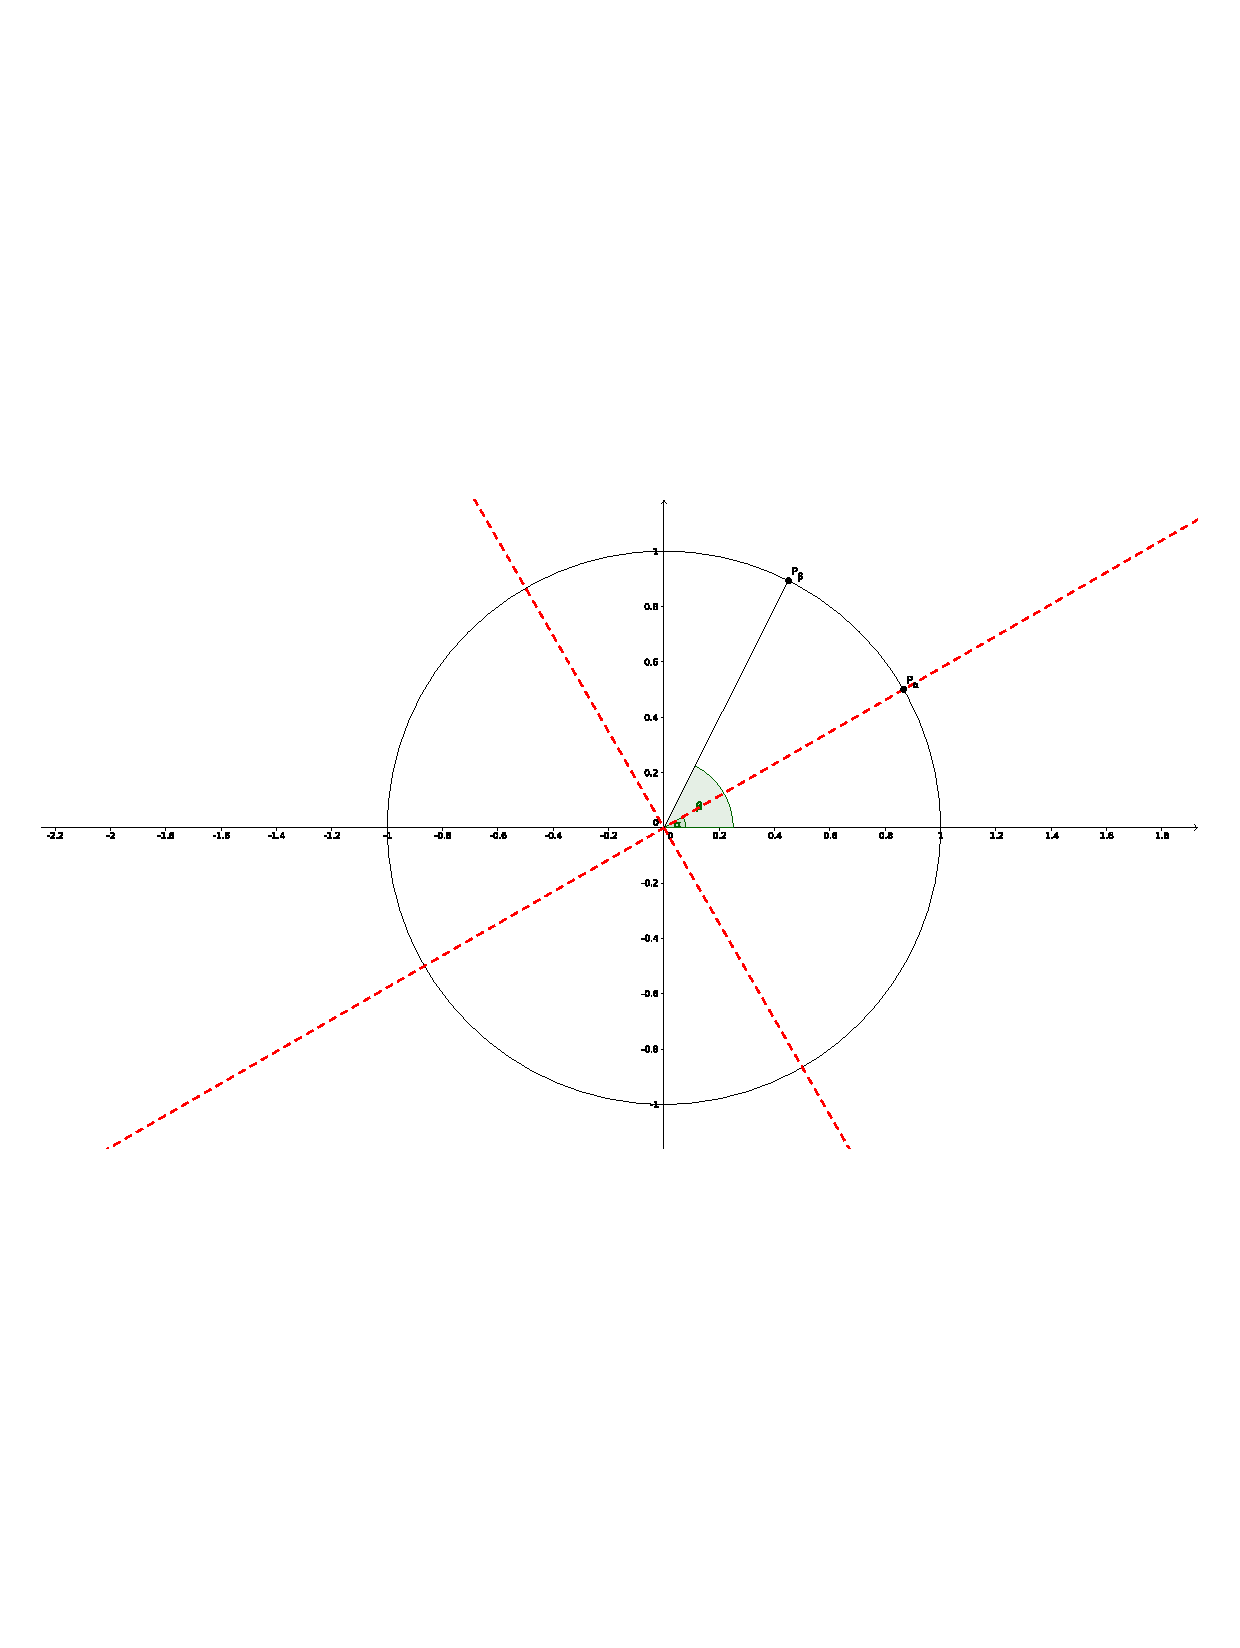
\includegraphics{cos_suma}}
\end{center}
Consideremos $\R^2$ con los ejes cartesianos, pero agreguemos otro par de ejes (en rojo) que corresponden a una rotación de los primeros en un ángulo $\alpha$. 
Las coordenadas del punto $P_{\alpha}$ con respecto a los ejes cartesianos son
$(\cos(\alpha),\sen(\alpha))$, mientras que sus coordenadas con
respecto a los ejes rotados son $(1,0)$.

Consideremos ahora un ángulo $\beta$ (en verde), las coordenadas de $P_{\beta}$ con respecto
a los ejes cartesianos son $(\cos(\beta),\sen(\beta))$ mientras que si se describen con respecto a los
ejes rotados son $(\cos(\beta-\alpha),\sen(\beta-\alpha))$. 

En general, si tomamos dos puntos: $(x_1,y_1)$ y $(x_2,y_2)$, la distancia que los separa se puede obtener por la fórmula:
$$dist((x_1,y_1),(x_2,y_2))=\sqrt{(x_1-x_2)^2+(y_1-y_2)^2}$$
Dado que la distancia entre
dos puntos de un plano no depende de las posiciones de los ejes respecto a los cuales se describen sus coordenadas, tenemos la siguiente igualdad.
\begin{eqnarray*}
 \textrm{medida según los ejes rotados}&=&\textrm{medida según los ejes cartesianos}\\
 (1-\cos(\beta-\alpha))^2 + 
	(0-\sen(\beta-\alpha))^2&=&	(\cos(\alpha)-\cos(\beta))^2 + (\sen(\alpha)-\sen(\beta))^2
\end{eqnarray*}
Si trabajamos esta igualdad, obtenemos lo siguiente.
\begin{eqnarray*}
1-2\cos(\beta-\alpha) + (\cos(\beta-\alpha))^2 + (\sen(\beta-\alpha))^2&=&
	(\cos(\alpha))^2-2\cos(\alpha)\cos(\beta) + (\cos(\beta))^2 +\\
	&& (\sen(\alpha))^2 - 2\sen(\alpha)\sen(\beta) + (\sen(\beta))^2\\
2-2\cos(\beta-\alpha)	-2\cos(\alpha)\cos(\beta) &=&
	  2- 2\sen(\alpha)\sen(\beta)  \\
\cos(\beta-\alpha)&=&\cos(\alpha)\cos(\beta) + \sen(\alpha)\sen(\beta) 
\end{eqnarray*}

\'Esta es una identidad trigonom\'etrica importante, nos da el valor del coseno de la resta de dos \'angulos
$\alpha$ y $\beta$ en t\'erminos de los senos y cosenos de $\alpha$ y $\beta$.

Podemos establecerla como una propiedad, junto con otras más que se desprenden de ella.

\begin{prop}
Dados $\alpha,\beta\in\R$, se cumplen las siguientes propiedades.
\begin{enumerate}
\item $\cos(\beta+\alpha)=\cos(\alpha)\cos(\beta) - \sen(\alpha)\sen(\beta)$
\item $\sen(\alpha + \beta)= \sen(\alpha)\cos(\beta) + \cos(\alpha)\sen(\beta)$
\item $\tan(\alpha + \beta) =  \frac{\tan(\alpha) + \tan(\beta)}{1-\tan(\alpha)\tan(\beta)}$
\item $\cos(2\alpha) = \cos(\alpha+\alpha) = (\cos(\alpha))^2 - (\sen(\alpha))^2$
\item $\sen(2\alpha) = 2\sen(\alpha)\cos(\alpha)$
\item $\tan(2\alpha) = \frac{2\tan(\alpha)}{1-(\tan(\alpha))^2}$
\end{enumerate}
\end{prop}

Las demostraciones se dejan de ejercicio, pero se basan en las identidades trigonométricas que vimos en la primera sección.



\chapter{Números Complejos}


Ya sabemos que el cuadrado de un numero real es siempre positivo, esto hace que la ecuación $x^2=-1$ no tenga solución, lo cual resulta molesto en muchos contextos. Nace entonces la necesidad de extender los reales a un conjunto más grande que sí dé cabida a la solución de esta ecuación.
La idea es extenderlo pero conservando las buenas propiedades algebraícas de ``cuerpo", al hacerlo se obtiene un nuevo cuerpo, que trae consigo un montón de propiedades inesperadas y abre la puerta a representar y resolver problemas que van mucho más allá de las ecuaciones, y resulta tener aplicaciones en la geometría, la trigonometría, la teoría de números y las ondas, entre otras.

\section{Definición y operatoria}

\begin{defn}
Considerando $i$ como una constante fija, se define el conjunto de los números complejos como:
\begin{equation}\label{ec0}
    \C=\{x+iy\ :\  x,y\in\R\}.
\end{equation} 
Se dota a este conjunto con operaciones de suma y multiplicación, las cuales se obtienen considerando la identidad $i^2=-1$, y asumiendo como verdaderas todas las propiedades de la suma y multiplicación de números reales.
\end{defn}

Notamos que $\R\subseteq\C$, ya que si tomamos $y=0$ obtenemos que $x+y i=x$, el cual puede ser tomado como cualquier número real.
Entonces este nuevo conjunto es una extensión de los números reales, tal como los racionales son una extensión de los enteros. 

Veamos cómo resultan las operaciones aritméticas en este conjunto. 
Para hacerlas nos valdremos de las propiedades de cuerpo y la identidad $i^2=-1$.
\begin{eqnarray*}
        (a+ib)+(c+id)&=&a+ib +c+id\\
        &=&a+c+ib +id\\
        &=&(a+c)+i(b+d)\label{ec1}
\end{eqnarray*}   
\begin{eqnarray*}
        (a+ib )(c+id)&=&a c+ia d+ib c+i^2b d\\
        &=&a c+ia d+ib c-b d\\
        &=&a c-b d+ia d+ib c\\
        &=&(a c-b d)+i(b c+a d)\label{ec2}
\end{eqnarray*}   

Resulta que las operaciones están bien definidas dentro de $\C$  ya que su resultado sigue siendo un objeto de $\C$.
Como se han definido a partir de las propiedades de cuerpo, podemos concluir que las respetan.

\medskip

\begin{prop}
La suma y la multiplicación en $\C$ cumplen las siguientes propiedades.
\begin{enumerate}
\item La suma es conmutativa
\item La suma es asociativa
\item $0\in\R$ es neutro para la suma
\item Para todo $a+ib\in\C$, $-a-ib$ es su inverso aditivo.
\item La multiplicación es conmutativa
\item La multiplicación es asociativa
\item $1\in\R$ es neutro para la multiplicación
\item\label{inverso} Para todo $a+ib\in\C$ no nulo, $\frac{a}{a^2+b^2}-i\frac{b}{a^2+b^2}$ es su inverso multiplicativo.
\item La multiplicación es distributiva respecto a la suma
\end{enumerate}
\end{prop}	
{\bf Demostración.} Son todas directas, salvo el ítem~\ref{inverso}, que verificaremos. Para hacerlo, basta multiplicar el número por quel que se propone como inverso, si resulta 1, es por que en efecto es el inverso multiplicativo.
\begin{eqnarray*}
			(a+ib)\left(\frac{a}{a^2+b^2}-i\frac{b}{a^2+b^2}\right)&=&\frac{(a+ib)(a-ib)}{a^2+b^2}\\
			&=&\frac{a^2-b(-b)+i(ab+a(-b))}{a^2+b^2}\\\\
			&=&\frac{a^2+b^2+i(ab-ab)}{a^2+b^2}\\
			&=&\frac{a^2+b^2}{a^2+b^2}\\
			&=&1
		\end{eqnarray*}
\hfill $\Box$

\subsection{Parte real e imaginaria de un número complejo}

\begin{defn}
Dado $z=a+ib \in\C$, con $a$, $b\in\R$, decimos que $a$ es la \emph{parte real de $z$}, y la denotamos por $\mbox{Re}(z)=a$.
Asimismo, el real que multiplica a $i$ lo llamamos \emph{parte imaginaria de $z$}, y lo denotamos por $\mbox{Im}(z)=b$.
Cuando un número complejo se expresa de esta forma, con $a$, $b\in\R$, decimos que se encuentra en \emph{forma binomial}.
\end{defn}
Con lo anterior se cumple lo siguiente.
$$z=\mbox{Re}(z)+i\mbox{Im}(z)$$
Con esta identidad, es fácil demostrar la siguiente propiedad.

\medskip

\begin{prop}
Dado un complejo $z$, se cumple que 
$$ z\in\R\Leftrightarrow Im(z)=0.$$
\end{prop}

\begin{ejemplo}
Para calcular la parte real e imaginara de un número complejo, debemos llevarlo a su forma estándar $a+ib$, donde $a,b\in\R$, de otra manera podemos caer en error.
    Calculemos la parte real y la parte imaginaria del siguiente número.
	$$\dfrac{1+i\sqrt{3}}{\sqrt{3}-i}+5i$$	
	Eliminamos la constante imaginaria del denominador mediante la técnica de racionalización.
	\begin{align*}
        \dfrac{1+i\sqrt{3}}{\sqrt{3}-i} &= 
            \left(\dfrac{1+i\sqrt{3}}{\sqrt{3}-i}\right)
            \cdot \left(\dfrac{\sqrt{3}+i}{\sqrt{3}+i}\right)
            = \dfrac{\sqrt{3}+i+3i+\sqrt{3}i^2}{3-i^2} = \dfrac{4i}{4} = i
	\end{align*}
	Ahora sumamos $5i$.
	\[
        \dfrac{1+i\sqrt{3}}{\sqrt{3}-i}+5i = i + 5i = 6i
	\]
	Así,
	\[
        \mbox{Re}\left(\dfrac{1+i\sqrt{3}}{\sqrt{3}-i}+5i\right) = 0,
        \qquad 
        \mbox{Im}\left(\dfrac{1+i\sqrt{3}}{\sqrt{3}-i}+5i\right) = 6.
	\]
\end{ejemplo}



\subsection{Conjugado de un número complejo}

\begin{defn}
El \emph{conjugado} de un número complejo $z=a+ib$, donde $a$, $b\in\R$, es un complejo que se denota por $\overline{z}$ y que se define como
$$ \overline{z}=a-ib.$$
 \end{defn}

\begin{prop}
Dados dos números complejos $z$, $w\in\C$ se cumplen las siguientes propiedades.
\begin{enumerate}
	\item Re$(z) = \mbox{Re}(\overline{z})$ y Im$(z) = - \mbox{Im}(\overline{z})$
	\item $z = \overline{z}$ si y solo si $z$ es real.
	\item $\overline{z + w} = \overline{z} + \overline{w}$.
	\item $\overline{z w} = \overline{z}  \overline{w}$.
        \item $\overline{z^{-1}}=\overline{z}^{-1}$.
	\item $z + \overline{z} = 2 \mbox{Re}(z)$.
	\item $z - \overline{z} = 2 i \mbox{Im}(z)$.
	\item $\overline{\overline{z}} = z$.
\end{enumerate}
\end{prop}
{\bf Demostración.}
\begin{enumerate}
	\item 
	En efecto, si $z=a+ib$, con $a$, $b\in\R$, entonces $\mbox{Re}(z)=a$ e $\mbox{Im}(z)=b$, por su parte $\overline{z}=a-ib$, por lo tanto $\mbox{Re}(\overline{z})=a=\mbox{Re}(z)$  e $\mbox{Im}(\overline{z})=-b=-\mbox{Im}(z)$.
	\item 	
	En efecto, si  $z = \overline{z}$, significa que $\mbox{Im}(z)=\mbox{Im}(\overline{z})$, pero usando la propiedad anterior esto se traduce en que $\mbox{Im}(z)=-\mbox{Im}(z)$, lo cual solo puede cumplirse si $\mbox{Im}(z)=0$, es decir solo si $z$ es real.
	\item	
	En efecto, si $z=a+ib$ y $w=x+iy$, con $a,b,x,y\in\R$, entonces 
	\begin{eqnarray*}
	\overline{z+w}&=&\overline{(a+ib)+(x+iy)}\\
	&=&\overline{(a+x)+i(b+y)}\\
	&=&(a+x)-i(b+y) \\
	&=&(a+x)+i(-b-y)\\
	&=&(a-ib)+(x-iy)\\
	&=&\overline{(a+ib)}+\overline{(x-iy)}\\
	&=& \overline{z} + \overline{w}.
	\end{eqnarray*}	
	\item 	
	En efecto, si $z=a+ib$ y $w=x+iy$, con $a,b,x,y\in\R$, entonces 
	\begin{eqnarray*}
	\overline{zw}&=&\overline{(a+ib)(x+iy)}\\
	&=&\overline{(ax-by)+i(bx+ay)}\\
	&=&(ax-by)-i(bx+ay)\\
	&=&(ax-by)+i(-bx-ay)\\
	&=&(ax-(-b)(-y))+i((-b)x+a(-y))\\
	&=&(a-ib)(x-iy)\\
	&=&\overline{(a+ib )}  \overline{(x+iy)}\\
	&=&\overline{z}  \overline{w}
	\end{eqnarray*}   
        \item
        En efecto, de la propiedad anterior tenemos que $1=\overline{1}=\overline{z z^{-1}} = \overline{z}  \overline{z^{-1}}$.
            Por lo tanto, $\overline{z}  \overline{z^{-1}} = 1 $, entonces $
            \overline{z^{-1}} = \overline{z}^{-1}$.	
	\item	
	En efecto, si $z=a+ib$, con $a$, $b\in\R$,  entonces
	\begin{eqnarray*}
	z + \overline{z}&=&(a+ib )+(a-ib)\\
	&=&(a+a)+i(b-b) \\
	&=&2a\\
	&=&2\mbox{Re}(z)
	\end{eqnarray*}
	\item
	En efecto, si $z=a+ib$, con $a$, $b\in\R$,  entonces
	\begin{eqnarray*}
	z - \overline{z}&=&(a+ib )-(a-ib)\\
	&=&(a+ib)+(-a+ib)\\
	&=&(a+(-a))+i(b+b))\\
	&=&2ib \\
	&=&2 i \mbox{Im}(z)
	\end{eqnarray*}
	\item
	En efecto, si $z=a+ib$, con $a$, $b\in\R$,  entonces
	\begin{eqnarray*}
	\overline{\overline{z}}&=&\overline{\overline{(a+ib)}}\\
	&=&\overline{(a-ib)}\\
	&=&(a+ib)\\
	\hspace{8cm}&=&z 	\hspace{7cm} \Box
	\end{eqnarray*}
\end{enumerate}


		
		\vspace{.5cm}
		
 \begin{ejercicio}{}{}
 Pruebe que para todo $z \in \C\setminus\{0\}$, se cumple que
 			\[
 				\overline{z + \frac 1 z} - \overline{\frac{1+z}{z}} = \overline{z}-1.
 			\]
 			\textbf{Soluci\'on:} Dado que
 			\begin{align*}
 				\overline{z + \frac 1 z} = \overline{z} + \overline{\frac 1 z}
 					= \overline{z} + \frac{1}{\overline{z}},\qquad\textrm{y}\qquad 
 				\overline{\frac{1+z}{z}} &= 
 					\frac{\overline{1+z}}{\overline{z}} = \frac{1 + \overline{z}}{\overline{z}}
 					= \frac{1}{\overline{z}} + 1,
 			\end{align*}
 			se tiene que 
			\begin{align*}
 				\overline{z + \frac 1 z} - \overline{\frac{1+z}{z}} =
 					\overline{z} + \frac{1}{\overline{z}} - \frac{1}{\overline{z}} - 1
 					= \overline{z} - 1.  	\hspace{7cm} \Box
 			\end{align*}
 \end{ejercicio}


%%%%%%%%%%%%%%%%%%%%%%%%%%%%%%%%%%%%%%%%%%%%%%%%%%%%%%%%%%%%%
%
%  capitulo plano de argand
%
%%%%%%%%%%%%%%%%%%%%%%%%%%%%%%%%%%%%%%%%%%%%%%%%%%%%%%%%%%%%%

\section{Representación en el plano de Argand}

Dado que un número complejo tiene una parte real y otra imaginaria, que son totalmente independientes entre sí, resulta práctico ver al número complejo como si fuera un \emph{par ordenado} de números reales.
En otras palabras, estamos diciendo que resulta práctico asociar a $z=a+b i\in\C$ con el par ordenado, o punto, $(a,b)\in\R\times\R$.
De esta forma, los números reales quedarían representados en el eje horizontal, y los números imaginarios quedarían en el eje vertical.

\begin{center}
\begin{tikzpicture}[scale=.7]
\draw[arrows=->] (-4.2,0) -- (4.2,0) node[right] {$\R$};
\draw[arrows=->] (0,-4.2) -- (0,4.2) node[above] {$\R$};
 \foreach \pos in {-4,-3,-2,-1,1,2,3,4}
    \draw[shift={(\pos,0)}] (0,.1) -- (0,-.1) node[below] {$\pos$};
 \foreach \pos in {-4,-3,-2,-1,1,2,3,4}
    \draw[shift={(0,\pos)}] (.1,0) -- (-.1,0) node[left] {$\pos$};
\draw[magenta,very thick,arrows=->] (0,0)--(2,0) node[above] {$2$};
\draw[blue,very thick,arrows=->] (0,0)--(0,3) node[right] {$3i$};
\draw[red,very thick,arrows=->] (0,0)--(1,1) node[right] {$1+i$};
\end{tikzpicture}
\end{center}

Con esta representación, la suma resulta totalmente natural.

\medskip

	
\begin{ejemplo}
Consideremos $z_1 = 1+2 i$ y $z_2 = 3-4 i$. 
La suma de ellos es el n\'umero complejo
\[
    z_1 + z_2 =(1+2 i) + (3-4 i) = (1 + 3) + (2-4) i = 4 -2 i,
\]
el cual coincide con la diagonal del paralelógramo definido por $z_1$ y $z_2$
\begin{center}
\begin{tikzpicture}[scale=.7]
\draw[arrows=->] (-4.2,0) -- (4.2,0) node[right] {$\R$};
\draw[arrows=->] (0,-4.2) -- (0,4.2) node[above] {$\R$};
 \foreach \pos in {-4,-3,-2,-1,1,2,3,4}
    \draw[shift={(\pos,0)}] (0,.1) -- (0,-.1) node[below] {$\pos$};
 \foreach \pos in {-4,-3,-2,-1,1,2,3,4}
    \draw[shift={(0,\pos)}] (.1,0) -- (-.1,0) node[left] {$\pos$};
\draw[magenta,very thick,arrows=->] (0,0)--(4,-2) node[right] {$4-2i$};
\draw[blue,very thick,arrows=->] (0,0)--(3,-4) node[right] {$3-4i$};
\draw[red,very thick,arrows=->] (0,0)--(1,2) node[right] {$1+2i$};
\draw[dashed] (3,-4)--(4,-2);
\draw[dashed] (1,2)--(4,-2);
\end{tikzpicture}
\end{center}
\end{ejemplo}

\subsection{Módulo de un número complejo}

Dado que estamos representando los números complejos como puntos en el plano; más aún, los estamos representando como flechas que van desde el origen hasta un determinado punto del plano, entonces puede ser interesante conocer el tamaño de esa flecha, en otras palabras, nos interesará conocer la distancia del origen del sistema cartesiano al punto que representa a $z$; tal magnitud la llamaremos \emph{módulo de $z$}. 

\medskip

\begin{defn}
    Dado un n\'umero complejo $z$, $z = a+ib $ con $a,b \in \R$, 
	se define el {\em m\'odulo de $z$} como el n\'umero real
	$$|z| = \sqrt{a^2+b^2}=\sqrt{(\textrm{Re}(z))^2+(\textrm{Im}(z))^2}.$$
\end{defn}
Recordemos que, si $z= a+ib$ es un complejo no nulo, entonces,
\begin{equation}\label{moduloconj}
	z^{-1} = \frac{a}{a^2+b^2}-i\frac{b}{a^2+b^2} = \frac{\left(a-ib\right)}{a^2+b^2}= \frac{\overline{z}}{|z|^2}.
\end{equation}
Esto es una interesante justificación para la introducción del concepto de conjugado.

\medskip

\begin{prop}
Dados dos complejos $z$, $w\in\C$ cualesquiera, se cumplen las siguientes propiedades.
\begin{enumerate}
\item $|z|\ge0$
\item $|z|=0$ si y solo si $z=0$
\item $|z|^2=z\overline{z}$
\item $|zw|=|z|\ |w|$
\item $|z^{-1}|=(|z|)^{-1}$
\item $|z+w|\le|z|+|w|$ {\bf (Desigualdad triangular)}
\item $|z|=|\overline{z}|$
\end{enumerate}
\end{prop}
{\bf Demostración.}
\begin{enumerate}
	\item 	
	En efecto, si $z=a+ib$, con $a,b\in\R$, entonces $|z|=\sqrt{a^2+b^2}$, y como $a,b\in\R$, entonces $a^2,b^2\ge 0$, así $a^2+b^2\ge 0$ y la raíz cuadrada se puede calcular, y por definición es un número mayor o igual a 0.
	\item 
	En efecto, si $z=a+ib$, con $a,b\in\R$, entonces 	
$$|z|=\sqrt{a^2+b^2}=0\Leftrightarrow {a^2+b^2}=0\Leftrightarrow a^2=0\wedge b^2=0\Leftrightarrow a=0\wedge b=0\Leftrightarrow z=0.$$
	\item De la ecuación~(\ref{moduloconj}), se obtiene directamente.
	\item 
	En efecto, basta observar, gracias a \eqref{moduloconj}, que
    \[
		|z w|^2 = z w \overline{z w} = z w \overline{z}  \overline{w} = z \overline{z} w \overline{w}
			= |z|^2 |w|^2.
    \]		
	\item 	
	En efecto, si $w = z^{-1}$ se tiene entonces que
            $|z| |z^{-1}| = |z z^{-1}| = |1| = 1$, es decir,
            $\left|z^{-1}\right| = \dfrac{1}{|z|} = |z|^{-1}$.
	\item Esta desigualdad no es tan simple de demostrar.
	Haremos uso de las siguientes propiedades: 
	\begin{itemize}
        \item para todo n\'umero real $x$ se cumple que $x \le |x|$.
        \item para todo n\'umero complejo $z = x + i y$ se tiene que 
            \[
                |\mbox{Re}(z)| = |x| = \sqrt{x^2} \le \sqrt{x^2 + y^2} = |z|.
            \]
	\end{itemize}
    Entonces,        
	\begin{align*}
        |z+w|^2 &= (z+w)(\overline{z+w}) \\
        &= (z+w)(\overline{z} + \overline{w})\\
              &  = |z|^2 + z\overline{w} + w\overline{z} + |w|^2\\
            &= |z|^2 + z\overline{w} + \overline{z\overline{w}} + |w|^2\\
                &= |z|^2 + 2\mbox{Re}(z\overline{w}) + |w|^2\\
            &\le |z|^2 + 2|\mbox{Re}(z\overline{w})| + |w|^2 \\
            &\le |z|^2 + 2|z\overline{w}| + |w|^2\\
            &= |z|^2 + 2|z|\ |\overline{w}| + |w|^2\\
            &= |z|^2 + 2|z|\ |w| + |w|^2\\
            &= \left(|z| + |w|\right)^2.
	\end{align*}
    Dado que se trata de n\'umeros reales no negativos, podemos extraer raíz cuadrada y concluir que:
    $$|z+w| \le |z| + |w|.$$
	\item 	
	En efecto, si $z=a+ib$, con $a,b\in\R$, entonces $\overline{z}=a-ib$, por lo tanto $|\overline{z}|=\sqrt{a^2+(-b)^2}=\sqrt{a^2+b^2}=|z|$.
\end{enumerate}

La última propiedad se visualiza en la siguiente figura, junto con la propiedad $|-z|=|z|$ la cual se obtiene de las anteriores tomando $w=-1$.

\begin{center}
\begin{tikzpicture}[scale=.7]
\draw[arrows=->] (-4.2,0) -- (4.2,0) node[right] {$\R$};
\draw[arrows=->] (0,-4.2) -- (0,4.2) node[above] {$\R$};
 \foreach \pos in {-4,-3,-2,-1,1,2,3,4}
    \draw[shift={(\pos,0)}] (0,.1) -- (0,-.1) node[below] {$\pos$};
 \foreach \pos in {-4,-3,-2,-1,1,2,3,4}
    \draw[shift={(0,\pos)}] (.1,0) -- (-.1,0) node[left] {$\pos$};
\draw[magenta,very thick,arrows=->] (0,0)--(-3,-1) node[left] {$z$};
\draw[blue,very thick,arrows=->] (0,0)--(-3,1) node[left] {$\overline{z}$};
\draw[red,very thick,arrows=->] (0,0)--(3,1) node[right] {$-z$};
\draw (0,0) circle (3.1623);
\end{tikzpicture}
\end{center}

La propiedades previas nos permiten hacer cálculos complicados sin necesidad de conocer la parte real o imaginaria del número, tal como el siguiente ejercicio muestra.

\begin{ejercicio}
Demuestre que:
$$\forall \in\C\setminus\{0\},\ \left|\dfrac{|z|}{z}-\overline{z}\right|=|1-|z|\, |.$$
En efecto, 
\begin{eqnarray*}
\left|\dfrac{|z|}{z}-\overline{z}\right|&=&\left|\dfrac{|z|-z\overline{z}}{z}\right|\\
&=&\left|\dfrac{|z|-|z|^2}{z}\right|\\
&=&\left|\dfrac{|z|(1-|z|)}{z}\right|\\
&=&|z|\left|\dfrac{1-|z|}{z}\right|\\
&=&|z|\dfrac{|1-|z||}{|z|}\\
&=&|1-|z| |
\end{eqnarray*}
\end{ejercicio}


%%%%%%%%%%%%%%%%%%%%%%%%%%%%%%%%%%%%%%%%%%%%%%%%%%%%%%%%%%%%%
%
%  forma polar
%
%%%%%%%%%%%%%%%%%%%%%%%%%%%%%%%%%%%%%%%%%%%%%%%%%%%%%%%%%%%%%

\section{Forma polar}

Valiéndonos de lo que aprendimos en trigonometría, podemos representar un número complejo $z$ en el plano cartesiano (o Plano de Argand) a través de su módulo, $|z|$, y del ángulo $\theta$ entre la semirecta positiva
del eje real y el vector asociado a $z$.

\begin{center}
\begin{tikzpicture}[scale=.7]
\draw[arrows=->] (-4.2,0) -- (4.2,0) node[right] {$\R$};
\draw[arrows=->] (0,-4.2) -- (0,4.2) node[above] {$\R$};
 \foreach \pos in {-4,-3,-2,-1,1,2,3,4}
    \draw[shift={(\pos,0)}] (0,.1) -- (0,-.1) node[below] {$\pos$};
 \foreach \pos in {-4,-3,-2,-1,1,2,3,4}
    \draw[shift={(0,\pos)}] (.1,0) -- (-.1,0) node[left] {$\pos$};
\draw[magenta,very thick,arrows=->] (0,0)-- (-1.5,1) node[above right] {$|z|$} -- (-3,2) node[above left] {$z$};
\draw (0,0) circle (3.6056);
\filldraw[fill=magenta!20,draw=magenta]
    (0,0) -- (1,0) arc (0:146.31:1) -- cycle;
\node[magenta] at (73.15:.5) {$\theta$};
\end{tikzpicture}
\end{center}

Entonces si $z=x+iy$ tenemos que:

\[
    x = |z| \cos(\theta),\qquad y = |z| \sen(\theta)
\]
y as\'i podemos escribir:
\begin{equation}\label{polar1}
    z = x + i y = |z| \cos(\theta) + i |z| \sen(\theta) = |z| \big(\cos(\theta) + i \sen(\theta)\big),
\end{equation}
siendo \'esta \'ultima la {\em representaci\'on
polar de $z$}, cuando $z \ne 0$.

Observe que, debido a la periodicidad de las funciones
seno y coseno, el n\'umero 
\[
    z = |z| \big(\cos(\theta) + i \sen(\theta)\big)
\]
tambi\'en podr\'ia ser escrito como 
\[
    z = |z| \big(\cos(\theta +2 \pi\big) + i \sen(\theta + 2 \pi)\big)
\]
o, de forma m\'as general, como 
\[
    z = |z| \big(\cos(\theta +2 k \pi) + 
    i \sen(\theta+2 k \pi)\big),\qquad k \in \Z.
\]

Para evitar que haya infinitas formas de representar a un n\'umero complejo
en forma polar, el valor de $\theta$ en la representaci\'on polar
de $z$ se restringe al intervalo $=\left]-\pi,\pi\right]$. 
Esto motiva la siguiente definici\'on.

\medskip 

\begin{defn}{}{}
Dado $z\neq 0$, se definen
\begin{itemize}
\item \textit{argumento de $z$}, que se denota $\text{arg}(z)$, como 
    el conjunto de todos los ángulos que definen $z$, es decir,
    $$\arg(z)=\big\{\theta\in\mathbb{R}:
         z=|z| \big(\cos(\theta)+i \sen(\theta)\big)\big\},$$
\item \textit{el argumento principal de $z$}, 
    denotado $\text{Arg}(z)$, como el \'unico     
    argumento de $z$ que pertenece al intervalo $]-\pi,\pi]$.
\end{itemize}
Si $z=0$, entonces decimos que $\arg(z)$ y $\text{Arg}(z)$ {\bf son indeterminados}.
\end{defn}


\medskip


\begin{prop}
    Para todo $z\in\mathbb{C}\setminus\{0\}$, se cumple:
    $$\arg(z)=\big\{\text{Arg}(z)+2 k \pi: k\in\mathbb{Z}\big\}.$$
\end{prop}

En la expresi\'on de un n\'umero complejo $z \ne 0$ en forma polar $z = |z| \big(\cos(\theta) + i \sen(\theta)\big)$
la suma $\cos(\theta) + i \sen(\theta)$ se abrevia como $\textrm{cis}(\theta)$ y, con esto, $z$ se re -- escribe como
\[
    z = |z| \mbox{cis}(\theta).
\]

Ya hemos practicado en las Evaluaciones 1 y 2 cómo determinar el ángulo entre un segmento y uno de los semiejes cartesianos, esto lo practicaremos muchísimo en este capítulo, veamos un ejemplo.

\begin{ejemplo}{}{}
Dado $z = 1 + i$ un n\'umero en forma binomial. 
            Para escribirlo en forma polar debemos determinar $|z|$ y
            Arg$(z)$,
            $$|z| = |1+i| = \sqrt{1+1} = \sqrt{2}.$$					
            Dado que el par ordenado $(1,1)$ asociado a $z$ 
            est\'a en el primer cuadrante,
            \[
                \mbox{Arg}(z) = \mbox{Arctan}(\frac{1}{1}) = \frac{\pi}{4}\in]-\pi,\pi].
            \]
            La representaci\'on polar de $z$ es entonces
            \[
                z = \sqrt{2}\left(\cos\left(\frac{\pi}{4}\right) + 
                    i \sen\left(\frac{\pi}{4}\right)\right)
                    = \sqrt{2}\ \mbox{cis}\left(\frac{\pi}{4}\right). 
            \]
\end{ejemplo}

\begin{ejemplo}{}{}
Dado $z = -3 i$ un imaginario puro ubicado en la parte  negativa del eje imaginario,
            \[
                \mbox{Arg}(z) = -\frac{\pi}{2},\quad |z| = 3
                \qquad \mbox{ y } \qquad
                z = 3 \mbox{cis}\left(-\frac{\pi}{2}\right).
            \]
\end{ejemplo}


\subsection{Igualdad en forma polar}

Dados $z_1 = |z_1| \mbox{cis}(\theta_1)$ y $z_2 = |z_2| \mbox{cis}(\theta_2)$,
se cumple que 
\begin{equation}\label{igualdadpolar}
    z_1 = z_2 \quad \gdw \quad |z_1| = |z_2| \quad \wedge \quad \exists k\in\Z,\ \theta_1 = \theta_2+2 k \pi.
\end{equation}

Por ejemplo,
\[
    2 \mbox{cis}\left(\frac{\pi}{6}\right)=
     2 \mbox{cis}\left(\frac{-23\pi}{6}\right)
\]

\subsection{Conjugado en forma polar}
Dado $z = |z| \mbox{cis}(\theta)$, entonces $\overline{z} = |z| \mbox{cis}(-\theta)$.

En efecto, como $z= |z| \cos(\theta) + i |z| \sen(\theta)$, entonces 
\begin{eqnarray*}
|z| \cos(-\theta) + i |z| \sen(-\theta)&=& |z| \cos(\theta) - i |z| \sen(\theta)\\
&=&\overline{z}.
\end{eqnarray*}

\subsection{Opuesto aditivo en forma polar}
Dado $z = |z| \mbox{cis}(\theta)$, entonces $-z = |z| \mbox{cis}(\theta+\pi)$.

En efecto, como $z= |z| \cos(\theta) + i |z| \sen(\theta)$, entonces 
\begin{eqnarray*}
|z| \cos(\theta+\pi) + i |z| \sen(\theta+\pi)&=& -|z| \cos(\theta) - i |z| \sen(\theta)\\
&=&-z.
\end{eqnarray*}

Observe que el valor $\theta+\pi$ puede no ser el argumento principal de $- z$.


\subsection{Inverso multiplicativo en forma polar}
Dado $z = |z| \mbox{cis}(\theta)\not=0$, entonces $z^{-1} = \frac{1}{|z|} \mbox{cis}(-\theta)$.

En efecto, ya vimos que si $z \ne 0$, su inverso multiplicativo es el n\'umero complejo
$$z^{-1} = \frac{1}{|z|^2}\overline{z}.$$
Como $z = |z| \mbox{cis}(\theta)$, entonces
\begin{eqnarray*}
    z^{-1} &=& \frac{1}{|z|^2} \overline{z}\\
        &=& \frac{1}{|z|^2}  |z| \mbox{cis}(- \theta)\\
        & =& \frac{1}{|z|} \mbox{cis}(- \theta).
\end{eqnarray*}




Consideremos $z_1 = |z_1| \mbox{cis}(\theta_1)$ y $z_2 = |z_2| \mbox{cis}(\theta_2)$ en $\C$.

\subsection{Multiplicación en forma polar}

La {\bf suma} no tiene una expresión simple en la forma polar, de hecho no es fácil calcular el argumento de la suma de dos complejos a partir del argumento de los sumandos

Sin embargo, es la {\bf mutiplicación} la que hace realmente interesante a la forma polar.
Desarrollemos:
\begin{eqnarray*}
    z_1 z_2 &=& (|z_1| \mbox{cis}(\theta_1))(|z_2| \mbox{cis}(\theta_2))\\
    &=& |z_1| (\cos(\theta_1)+i \sen(\theta_1))|z_2| (\cos(\theta_2)+i \sen(\theta_2))\\
    &=& |z_1| |z_2| \big[\cos(\theta_1) \cos(\theta_2)-\sen(\theta_1) \sen(\theta_2)
    + i \big(\sen(\theta_1) \cos(\theta_2) + \cos(\theta_1) \sen(\theta_2)\big)\big],\\
\end{eqnarray*}
Pero esta expresión con productos de senos y cosenos está relacionada con el coseno $\cos(\theta_1+\theta_2)$ y $\sen(\theta_1+\theta_2)$, tal como establece el siguiente teorema.

\medskip

\begin{thm}
Dados dos ángulos cuales quiera $\theta_1$, $\theta_2\in\R$, se cumple:
$$\cos(\theta_1+\theta_2)=\cos(\theta_1) \cos(\theta_2)-\sen(\theta_1) \sen(\theta_2)\textrm{ y }\sen(\theta_1+\theta_2)=\sen(\theta_1) \cos(\theta_2) + \cos(\theta_1) \sen(\theta_2)$$
\end{thm}
{\bf Demostración} La siguiente figura es una prueba gráfica para el caso en que tanto $\theta_1$, $\theta_2$ como $\theta_1+\theta_2$ están $[0,\pi/2]$.

\begin{center}
\begin{tikzpicture}[scale=2]
\draw (0,0) -- (4,0) node[midway,below] {$\cos(\theta_2)\cos(\theta_1)$}--(4,4.5) -- (0,4.5)--
	cycle node[midway,sloped,above]  {$\sen(\theta_1+\theta_2)$};
\draw (0,0) -- (4,2.5) node[midway,above left,sloped] {$\cos(\theta_2)$};
\node[below,rotate=90] at (4,1) {$\cos(\theta_2)\sen(\theta_1)$};
\draw (4,2.5)--(2.75,4.5) node[midway,above left,sloped] {$\sen(\theta_2)$}--(0,0) node[midway,above left] {1};
\node[below,rotate=90] at (4,3.5) {$\cos(\theta_1)\sen(\theta_2)$};
\node[above] at (3.4,4.5) {$\sen(\theta_2)\sen(\theta_1)$};
\draw (3.75,2.9)--++(-.4,-.25)--++(.25,-.4);
\draw (4,3.5) arc (90:122.005:1);
\node at (3.84,3.3) {\small$\theta_1$};
\draw (1,0) arc (0:32.005:1);
\node at (16:.8) {\small$\theta_1$};
\draw (32.005:1) arc (32.005:58.570:1);
\node at (45:.8) {\small$\theta_2$};
\node[above] at (1.375,4.5) {$\cos(\theta_1+\theta_2)$};
\draw (1.75,4.5) arc (180:238.57:1);
\node at (2.2,4.3) {\small$\theta_1+\theta_2$};
\end{tikzpicture}
\end{center}

Los demás casos se pueden obtener con bastante trabajo usando las simetrías e identidades vistas al comienzo del curso.
\hfill $\Box$

Esto da lugar a la siguiente hermosa y sintética fórmula.
\begin{eqnarray*}
   z_1 z_2  &=& |z_1| |z_2| \big(\cos(\theta_1+\theta_2)+i \sen(\theta_1+\theta_2)\big)\\
    &=& |z_1| |z_2| \mbox{cis}(\theta_1+\theta_2).
\end{eqnarray*}
También la división funciona muy bien.
\begin{align*}
    \frac{z_1}{z_2} &=  \frac{|z_1|}{|z_2|} \mbox{cis}(\theta_1-\theta_2).				
\end{align*}
Esto da una representaci\'on gr\'afica para el producto $z_1z_2$, usando trigonometría y triángulos semejantes.
\begin{ejemplo}
    Calculemos $z_1 z_2$ con
    \[
        z_1 = - \sqrt{3}+i,\qquad z_2 =\frac{1+ i}{2}.
    \]
    Dado que 
    \[
        z_1 = 2 \mbox{cis}\left(\frac{5 \pi}{6}\right),\qquad
        z_2 = \frac{\sqrt{2}}{2}\mbox{cis}\left(\frac\pi 4\right),
    \]
    su producto puede calcularse como 
    $$z_1 z_2 = \sqrt{2}\ \mbox{cis}\left(\frac{5 \pi}{6}+\frac\pi 4\right)=  \sqrt{2}\ \mbox{cis}\left(\frac{13 \pi}{12}\right)= 
         \sqrt{2}\ \mbox{cis}\left(-\frac{11 \pi}{12}\right).$$
        
\begin{center}
\begin{tikzpicture}
\draw[arrows=->] (-2.2,0) -- (2.2,0);
\draw[arrows=->] (0,-2.2) -- (0,2.2);
 \foreach \pos in {-2,-1,1,2}
    \draw[shift={(\pos,0)}] (0,.1) -- (0,-.1) node[below] {\tiny $\pos$};
 \foreach \pos in {-2,-1,1,2}
    \draw[shift={(0,\pos)}] (.1,0) -- (-.1,0) node[left] {\tiny $\pos$};

\draw[red,very thick,arrows=->] (0,0)-- (150:2)  node[left] {$2 \textrm{cis}(5\pi/6)$};
\filldraw[fill=blue!20!white,draw=blue]
    (0,0) -- (0.5,0) -- (45:0.7071) -- cycle;

\draw[blue,very thick,arrows=->] (0,0)-- (45:0.7071)  node[above right] {$\sqrt{2}/2\ \textrm{cis}(\pi/4)$};
\filldraw[fill=blue!20!white,draw=blue]
    (0,0) -- (150: 1) -- (195:1.4142) -- cycle;

\draw[magenta,very thick,arrows=->] (0,0)-- (-165:1.4142)  node[below left] {$\sqrt{2}\ \textrm{cis}(-11\pi/12)$};
\end{tikzpicture}
\end{center}


\end{ejemplo}

\subsection{Teorema de De Moivre: cálculo de potencias en forma polar} 

Dado que la multiplicación se simplifica tanto con la forma polar, lo mismo ocurre con las potencias enteras.		
Dados $z \in \C$ y $n \in \N$, la potencia con exponente natural $n$ de $z$ resulta tener la siguiente fórmula.

$$    z^n = |z|^n \mbox{cis}(n \theta).$$
    
La cual recibe el nombre de {\em F\'ormula de De Moivre}.
    
 La demostración se hace formalmente por inducción, pero proviene directamente de la fórmula de la multiplicación, en la cual el módulo de la multiplicación es la multiplicación de los módulos y el argumento de la multiplicación es la suma de los argumentos.

\begin{ejemplo}{}{}
    Calculemos  $(1+i)^4$.
    
    \begin{itemize}
        \item Podemos utilizar la f\'ormula del binomio,
        \[
            (1+i)^4 = 1 + 4 i + 6 i^2 + 4 i^3 + i^4 = 
                1 + 4 i - 6 - 4 i + 1 = - 4.
        \]
        
        \item Podemos escribir a $1+i$ en forma polar y utilizar la f\'ormula anterior
        \[
            1 + i = \sqrt{2} \mbox{cis}\left(\frac{\pi}{4}\right) 
            \quad \Longrightarrow \quad (1+i)^4 = 
            \big( \sqrt{2} \big)^4 \mbox{cis}\left(4 \frac{\pi}{4}\right) 
            = 4 \mbox{cis}(\pi)
            =4 \cos(\pi) + 4 i \sin(\pi) = - 4
        \]
        Comprobamos que llegamos al mismo resultado
    \end{itemize}
        
    La siguiente figura muestra sucesivamente: $(1+i)^{-1}$, $(1+i)^{0}$, $(1+i)$, $(1+i)^{2}$, $(1+i)^{3}$, $(1+i)^{4}$.
        
\begin{center}
\begin{tikzpicture}

\draw[magenta,very thick,arrows=->] (0,0)-- (45:1.4142)  node[above right] {$\sqrt{2}\ \textrm{cis}(\pi/4)$};
\draw[blue,very thick,arrows=->] (0,0)-- (90:2)  node[above right] {$2\ \textrm{cis}(\pi/2)$};
\draw[green!50!black,very thick,arrows=->] (0,0)-- (135:2.8284)  node[left] {$2\sqrt{2}\ \textrm{cis}(3\pi/4)$};
\draw[red,very thick,arrows=->] (0,0)-- (180:4)  node[left] {$4\ \textrm{cis}(\pi)$};
\draw[yellow!50!black,very thick,arrows=->] (0,0)-- (0:1)  node[right] {$\textrm{cis}(0)$};
\draw[orange,very thick,arrows=->] (0,0)-- (-45:0.7071)  node[below right] {$(1/\sqrt{2})\ \textrm{cis}(-\pi/4)$};
\end{tikzpicture}
\end{center}


    
\end{ejemplo}

\medskip 


Análogamente, $z^{-n}$ puede calcularse mediante
\[
    \left(z^{-1}\right)^n = 
    \left(\left( |z| \mbox{cis}(\theta) \right)^{-1}\right)^n
    = \left(\frac{1}{|z|} \mbox{cis}(- \theta)\right)^n
    = \frac{1}{|z|^n} \mbox{cis}(- n \theta)=|z|^{-n} \mbox{cis}(- n \theta).
\]


\begin{ejercicio}{}{}
    Calcule y escriba el resultado en forma polar de $(1+\sqrt{3} i)^{200}$.
    
\begin{eqnarray*}
(1+\sqrt{3} i)^{200} &=& \left(2 \mbox{cis}\left(\frac \pi 3\right)\right)^{200}\\
            &=& 2^{200} \mbox{cis}\left(\frac{200\pi}{3}\right)\\
            &=& 2^{200}\mbox{cis}\left(\frac{(3\cdot 66 + 1) \pi}{3}\right)\\
                &=& 2^{200}\mbox{cis}\left(66 \pi + \frac{\pi}{3}\right)\\
                &=& 2^{200}\mbox{cis}\left(33\cdot 2 \pi + \frac{\pi}{3}\right)\\
                &=& 2^{200}\mbox{cis}\left(\frac{\pi}{3}\right)
\end{eqnarray*}
\end{ejercicio}

\section{Ra\'ices de un número complejo}


En los reales solo considerábamos la raíz cuadrada positiva de un número positivo, descartando su opuesto aditivo que sin embargo daba el mismo resultado al elevarse al cuadrado. 
En el conjunto de los números complejos nos abriremos a considerar varias raíces, partiendo de la siguiente definición.

\begin{defn}{}{}
Dado $z \in \C$, y $n \in \N$, decimos que $w\in\C$ es una  {\em ra\'{\i}z $n$-\'esima de $z$}
si cumple que $w^n = z$.
\end{defn}


Con esta definición tanto 2 como -2 son raíces cuadradas de 4, ya no hablamos de \emph{la} raíz de 4 sino de \emph{las} raíces.


También tenemos que tanto $i$ como $-i$ son raíces cuadradas de $-1$.
Por lo tanto vemos también que tanto $1$ como $-1$, $i$ y $-i$ sin todas raíces cuartas de $1$, ya que 

$$ 1^4=(-1)^4=i^4=(-i)^4=1.$$

Por otra parte, observamos que solo 0 es raíz de 0, este número tiene solo una raíz.

?`C\'omo determinar una ra\'iz $n$-\'esima $w$ de un $z$ dado?
Hay muchas maneras, pero dado que fue sencillo calcular las potencias de un número en forma polar, será también sencillo calcular sus raíces en forma polar, veamos.
Supongamos que 
$z = |z| \mbox{cis}(\theta_z)$ y queremos determinar 
$w$ en forma polar $|w| \mbox{cis}(\theta_w)$ de manera tal que $w^n = z$.
 
Como $w^n = |w|^n \mbox{cis}(n \theta_w)=|z| \mbox{cis}(\theta_z)$,
se cumple si y s\'olo si,
\begin{align*}
    |w|^n=|z| \textrm{ y existe } k\in \Z \textrm{ tal que } n \theta_w=\theta_z +2k\pi,
\end{align*}
o, equivalentemente,
\begin{align*}
    |w|=\sqrt[n]{|z|} \textrm{ y existe } k\in \Z \textrm{ tal que } \theta_w=\frac{\theta_z}{n} +\frac{ 2 k  \pi}{n}
\end{align*}
de manera que en principio no hay una si no infinitas raíces... pero ¿será realmente así? ¿qué pasa cuando tomamos $k=n$?
$$\theta_w=\frac{\theta_z}{n} +\frac{ 2 n  \pi}{n}=\frac{\theta_z}{n}+2 \pi$$
el cual es equivalente al argumento $\dfrac{\theta_z}{n}$, el cual se obtiene tomando $k=0$.

En general tendremos que tomar $k+n$ es equivalente a tomar $k$, así $z$ solo tiene $n$ raíces:
\begin{align*}
    w_k=\sqrt[n]{|z|} cis \left(\frac{\theta_z}{n} +\frac{ 2 k  \pi}{n}\right), \textrm{ con } k\in\{0,1,\dots,n-1\}
\end{align*}

Lo anterior permite inferir el siguiente resultado:

\begin{lem}{}{}
    Para todo $z \in \C$, $z\neq 0$, se cumple que 
    $z$ tiene $n$ ra\'{\i}ces $n$-\'esimas distintas entre s\'{\i}. 
    Si $z = |z| \mbox{cis}(\theta)$, entonces estas son:
    \begin{equation}\label{raicesz}
        \left\{
            |z|^{1/n} \mbox{cis}\left(\frac{\theta}{n} + 
            \frac{2 j \pi}{n}\right)\;:\;
            j \in \{0,1,2,\ldots, n-1\}
        \right\}
    \end{equation}
\end{lem}


\begin{prueba}
    Seg\'un se vio antes, las ra\'ices $n$-\'esimas de 
    $z = |z| \mbox{cis}(\theta)$ son los
    n\'umeros complejos de la forma
    \[
       |z|^{\frac 1 n} 
            \mbox{cis}\left(\frac{\theta}{n} + 2 \pi \frac{k}{n}
            \right)\;:\; k \in \Z
    \]
    Cualquier n\'umero natural $k$ deja resto entre 0 y $n-1$ al dividirlo por $n$, por tanto,
    cualquer n\'umero entero $k$ puede escribirse
    como 
    \[
        k = m n + j,\qquad \mbox{ con } m \in \Z \quad \wedge \quad j \in \{0,1,2,\cdots,n-1\}.
    \]
    Entonces, las ra\'ices $n$ -- \'esimas de $z$ están dadas por:
    \[
        \left\{|z|^{\frac 1 n} \mbox{cis}\left(\frac{\theta}{n} + 
            2 \pi \frac{m n+j}{n}\right)\;:\;m \in \Z \quad \wedge \quad j \in \{0,1,2,\cdots,n-1\}\right\}.
    \]
    Reemplazando $m$ por $0$ se obtienen los valores en \eqref{raicesz}. 
    Ahora, para cada $j \in \{0,1,2,\ldots,n-1\}$ sea 
    $w_j = |z|^{1/n} \mbox{cis}\left(\frac{\theta}{n} + \frac{2 j \pi}{n}\right)$,
    con lo cual se obtiene la siguiente descomposici\'on,
    \[
            \underbrace{\left\{w_0,  w_1,  \cdots,  w_{n-1}\right\}}_{=: {\mathcal R}_1}
            \;\bigcup\; 
            \underbrace{\left\{|z|^{\frac 1 n} \mbox{cis}\left(\frac{\theta}{n} + 
            2 \pi \frac{m n+j}{n}\right)\;:\; m \in \Z-\{0\} \quad \wedge \quad
            j \in \{0,1,2,\cdots,n-1\}\right\}}_{=: {\mathcal R}_2}.
    \]    
    Si $w \in {\mathcal R}_2$, existen $m \in \Z-\{0\}$ y $j \in \{0,1,\cdots,n-1\}$
    de modo que 
    \[
       w = |z|^{\frac 1 n} \mbox{cis}\left(\frac{\theta}{n} + 
            2 \pi \frac{m n+j}{n}\right)
            =
            |z|^{\frac 1 n} \mbox{cis}\left(\frac{\theta}{n} + 2 \pi m + 2 \pi \frac{j}{n}\right).
    \]
    Debido a que las funciones seno y coseno son peri\'odicas de per\'iodo
    $2 \pi$ se tiene que 
    \[
        w = |z|^{\frac 1 n} \mbox{cis}\left(\frac{\theta}{n} + 2 \pi m + 2 \pi \frac{j}{n}\right)
        = |z|^{\frac 1 n} \mbox{cis}\left(\frac{\theta}{n} + 2 \pi \frac{j}{n}\right)
        = w_j.
    \]
    Es decir, cada elemento $w \in {\mathcal R}_2$ es igual a alguno de los $n$ elementos
    en ${\mathcal R}_1$, y as\'i, las ra\'ices $n$ -- \'esimas de $z$ es,
    por tanto, el conjunto ${\mathcal R}_1$.   
\end{prueba}



\begin{ejemplo}{}{}
    Calculemos las ra\'{\i}ces cuadradas de $1+i\sqrt{3} =  2 \mbox{cis}\left(\frac \pi 3\right)$.
        
    Los n\'umeros complejos de la forma
    \[
        2^{1/2} \mbox{cis}\left(\frac \pi 6 + k \pi\right)
    \]
    con $k \in \{0,1\}$ son ra\'ices cuadradas de $1+i\sqrt{3}$. 
     
    Demos valores a $k$ y veamos qu\'e n\'umeros complejos   son ra\'ices cuadradas de $1 +i \sqrt{3}$.    
    \begin{itemize}
        \item con $k = 0$: $\sqrt{2} \mbox{cis}\left(\frac \pi 6\right)$. 
            Llam\'emosle $w_0$.
            
        \item con $k = 1$: 
            $\sqrt{2} \mbox{cis}\left(\frac \pi 6 + \pi\right) =
            \sqrt{2} \mbox{cis}\left(\frac{7 \pi}{6}\right) = 
            \sqrt{2} \mbox{cis}\left(-\frac{5 \pi}{6}\right)$.
            Llam\'emosle $w_1$.
       \item con $k=2$: $\sqrt{2} \mbox{cis}\left(\frac \pi 6 + 2 \pi\right)$,
            que es igual al valor que obtuvimos con $k=0$,
            es decir, es igual a $w_0$.
       \item con $k = 3$:  $\sqrt{2} \mbox{cis}\left(\frac \pi 6 + 3 \pi\right)
            = \sqrt{2} \mbox{cis}\left(\frac \pi 6 + \pi\right) 
            = \sqrt{2} \mbox{cis}\left(\frac \pi 6 + \pi - 2 \pi\right)$,
            y es igual al valor que obtuvimos con $k=1$, que denominamos
            $w_1$.
    \end{itemize}
    Por lo tanto $1+i\sqrt{3}$ tiene solo dos raíces cuadradas: $w_0$ y $w_1$.
    
    
\begin{center}
\begin{tikzpicture}
\draw[arrows=->] (-2.2,0) -- (2.2,0);
\draw[arrows=->] (0,-2.2) -- (0,2.2);
 \foreach \pos in {-2,-1,1,2}
    \draw[shift={(\pos,0)}] (0,.1) -- (0,-.1) node[below] {$\pos$};
 \foreach \pos in {-2,-1,1,2}
    \draw[shift={(0,\pos)}] (.1,0) -- (-.1,0) node[left] {$\pos$};
\draw[magenta,very thick,arrows=->] (0,0)-- (60:2)  node[above right] {$2\textrm{cis}(\pi/3)$};
\draw[blue,very thick,arrows=->] (0,0)-- (30:1.4142)  node[above right] {$\sqrt{2}\textrm{cis}(\pi/6)$};
\draw[red,very thick,arrows=->] (0,0)-- (-150:1.4142)  node[below left] {$\sqrt{2}\textrm{cis}(-5\pi/6)$};
\end{tikzpicture}
\end{center}
\end{ejemplo}     
               
\begin{ejemplo}{}{} 
    Determinemos las ra\'{\i}ces cuartas de 
    $i = \mbox{cis}\left(\frac \pi 2 \right)$.
    
    De lo anterior, tenemos que estas son:
    $$w = \mbox{cis}\left(\frac \pi 8 + \frac{2k \pi}{ 4} \right)= \mbox{cis}\left(\frac \pi 8 + k\frac \pi 2 \right),$$    
    con $k$ tomando valores $0, 1, 2, 3$.
    \begin{align*}
        w_0 &= \mbox{cis}\left(\frac \pi 8\right)\; &\mbox{ con } 
        k &= 0,\\
        w_1 &= \mbox{cis}\left(\frac{5 \pi}{8}\right)\; &\mbox{ con } 
        k &= 1,\\
        w_2 &= \mbox{cis}\left(\frac{9 \pi}{8}\right) =
            \mbox{cis}\left(-\frac{7 \pi}{8}\right),\; &\mbox{con } 
            k &= 2,\\
        w_3 &= \mbox{cis}\left(\frac{13 \pi}{8}\right) =
            \mbox{cis}\left(-\frac{3 \pi}{8}\right),\; &\mbox{ con  } 
            k &= 3.
    \end{align*}
    
\begin{center}
\begin{tikzpicture}[scale=2]
\draw[arrows=->] (-1.2,0) -- (1.2,0);
\draw[arrows=->] (0,-1.2) -- (0,1.2);
 \foreach \pos in {-1,1}
    \draw[shift={(\pos,0)}] (0,.1) -- (0,-.1) node[below] {$\pos$};
 \foreach \pos in {-1,1}
    \draw[shift={(0,\pos)}] (.1,0) -- (-.1,0) node[left] {$\pos$};
\draw[magenta,very thick,arrows=->] (0,0)-- (90:1)  node[above right] {$\textrm{cis}(\pi/2)$};
\draw[blue,very thick,arrows=->] (0,0)-- (22.5:1)  node[above right] {$\textrm{cis}(\pi/8)$};
\draw[red,very thick,arrows=->] (0,0)-- (112.5:1)  node[below left] {$\textrm{cis}(5\pi/8)$};
\draw[green,very thick,arrows=->] (0,0)-- (-67.5:1)  node[above right] {$\textrm{cis}(-7\pi/8)$};
\draw[orange,very thick,arrows=->] (0,0)-- (-157.5:1)  node[below left] {$\textrm{cis}(-3\pi/8)$};
\end{tikzpicture}
\end{center}

\end{ejemplo}

Los reales también adquirirán muchas raíces nuevas según esta nueva definición, en general, todo numero, real o complejo, tendrá exactamente $n$ raíces $n$-ésimas distintas.
En particular las raíces $n$-ésimas de $z=1$ son:
$$ u_k=\mbox{cis}\left(\frac{2k\pi}{n}\right),\textrm{ con }k\in\{0,1,\dots,n-1\}.$$


\begin{center}
\begin{tikzpicture}
  \draw[arrows=->,color=blue!50!red] (-6,0) -- ++ (120:2);
  \draw[arrows=->,color=blue!50!red] (-6,0) -- ++(0:2);
  \draw[arrows=->,color=blue!50!red] (-6,0) -- ++ (-120:2);
  \node at (-6,3) {Las 3 raíces 3-ésimas de 1};


  \draw[arrows=->,color=blue!50!red] (0,0) -- ++ (90:2);
  \draw[arrows=->,color=blue!50!red] (0,0) -- ++(0:2);
  \draw[arrows=->,color=blue!50!red] (0,0) -- ++ (-90:2);
  \draw[arrows=->,color=blue!50!red] (0,0) -- ++ (180:2);
  \node at (0,3) {Las 4 raíces 4-ésimas de 1};

  
  \draw[arrows=->,color=blue!50!red] (6,0) -- ++ (72:2);
  \draw[arrows=->,color=blue!50!red] (6,0) -- ++(0:2);
  \draw[arrows=->,color=blue!50!red] (6,0) -- ++ (144:2);
  \draw[arrows=->,color=blue!50!red] (6,0) -- ++ (-144:2);
  \draw[arrows=->,color=blue!50!red] (6,0) -- ++ (-72:2);
  \node at (6,3) {Las 5 raíces 5-ésimas de 1};
\end{tikzpicture}
\end{center}

Pasa un fenómeno muy interesante cuando sumamos las $n$-ésimas raíces de la unidad:

\begin{center}
\begin{tikzpicture}
  \draw[arrows=->,color=blue!50!red] (-6,0) -- ++(0:2)-- ++ (120:2)-- ++ (-120:2);

  \draw[arrows=->,color=blue!50!red] (0,0) -- ++(0:2)-- ++ (90:2) -- ++ (180:2)-- ++ (-90:2);
 

  
  \draw[arrows=->,color=blue!50!red] (6,0) -- ++(0:2)-- ++ (72:2)-- ++ (144:2)-- ++(-144:2)-- ++ (-72:2);
\end{tikzpicture}
\end{center}

¡¡Las raíces $n$-ésimas de la unidad conforman un polígono regular de $n$ lados!! y dado que se trata de un polígono cerrado, su suma es cero siempre. 

Pero lo más interesante es las raíces de 1 es que nos permiten obtener las raíces de todos los demás números complejos.
\begin{lem}{}{}
    Sean $n\in\N$ y $z \in \C$ tal que $z=|z|\mbox{cis}(\theta_z) \ne 0$, y sean $u_0,\dots , u_{n-1}$ las raíces $n$-ésimas de 1.
    Entonces, las ra\'{\i}ces $n$ -- \'esimas de $z$ son:
    \[
        \sqrt[n]{|z|} \mbox{cis}\left(\frac{\theta_z}{n}\right)u_0,\sqrt[n]{|z|} \mbox{cis}\left(\frac{\theta_z}{n}\right) u_1,  \cdots, \sqrt[n]{|z|} \mbox{cis}\left(\frac{\theta_z}{n}\right)u_{n-1}.
    \]
\end{lem}



\begin{prueba}
Sabemos que las raíces $n$-ésimas de $z$ son:
$$\sqrt[n]{|z|} \mbox{cis}\left(\frac{\theta_z}{n}+\frac{2 k \pi}{n}\right),\mbox{ con } k\in\{0,1,\dots,n-1\}$$
Sea $k\in\{0,1,\dots,n-1\}$ fijo, observemos lo siguiente:
$$\sqrt[n]{|z|} \mbox{cis}\left(\frac{\theta_z}{n}+\frac{2 k \pi}{n}\right)=\sqrt[n]{|z|} \mbox{cis}\left(\frac{\theta_z}{n}\right)\mbox{cis}\left(\frac{2 k \pi}{n}\right)=\sqrt[n]{|z|} \mbox{cis}\left(\frac{\theta_z}{n}\right)u_k$$
Con lo cual queda demostrado lo afirmado.
\end{prueba}

\begin{center}
\begin{tikzpicture}
  \draw[arrows=->,color=blue!50!red] (0,0) -- ++ (15:2) node[above] {$\sqrt[12]{2}\mbox{cis}\left(\frac{\pi}{24}\right)$};
  \draw[arrows=->,color=blue!50!red] (0,0) -- ++ (75:2) node[above] {$\sqrt[12]{2}\mbox{cis}\left(\frac{\pi}{24}+\frac{\pi}{3}\right)$};
  \draw[arrows=->,color=blue!50!red] (0,0) -- ++(135:2) node[above] {$\sqrt[12]{2}\mbox{cis}\left(\frac{\pi}{24}+2\frac{\pi}{3}\right)$};
  \draw[arrows=->,color=blue!50!red] (0,0) -- ++ (195:2) node[below] {$\sqrt[12]{2}\mbox{cis}\left(\frac{\pi}{24}+\pi\right)$};
  \draw[arrows=->,color=blue!50!red] (0,0) -- ++ (255:2) node[below] {$\sqrt[12]{2}\mbox{cis}\left(\frac{\pi}{24}+4\frac{\pi}{3}\right)$};
  \draw[arrows=->,color=blue!50!red] (0,0) -- ++ (315:2) node[below] {$\sqrt[12]{2}\mbox{cis}\left(\frac{\pi}{24}+5\frac{\pi}{3}\right)$};
  \node at (0,4) {Las 6 raíces 6-ésimas de 1+i};
 \end{tikzpicture}
\end{center}

\medskip

\begin{cor}{}{}
    Para todo n\'umero complejo $z$ se cumple que la suma de sus 
    ra\'{\i}ces $n$ -- \'esimas es cero.
\end{cor}

\subsection{Ejercicios}

Terminamos este apunte con dos ejercicios.

\begin{ejercicio}{}{}
    \begin{enumerate}
        \item Resuelva en $\C$ y en $\R$ la ecuaci\'on $x^2 + 2x + 4 = 0$.
        \item Resuelva en $\C$ la ecuaci\'on 
        $\displaystyle z^2 + \frac 1 z = 0$.
    \end{enumerate}
    \vspace{0.3cm}
    \textbf{Soluci\'on:}
    \begin{enumerate}
        \item 
            Procedamos a completar cuadrados.
            \begin{align*}
                0 = x^2 + 2 x + 4\quad & \gdw \quad 0 = (x^2 + 2 x + 1) + 4 - 1
                \quad \gdw \quad (x+1)^2 = - 3,
            \end{align*}
            Si $x \in \R$, entonces $(x+1)^2 \ge 0$ y 
            la ecuaci\'on anterior
            no tiene soluci\'on.\\
            
            Si $x \in \C$, la ecuaci\'on $(x+1)^2 = - 3$ 
            es equivalente a que 
            $x+1$ sea una de las ra\'ices cuadradas de $- 3$, es decir, dado que $- 3=3\mbox{cis}(\pi)$
            \begin{align*}
                x+1 \in &\left\{ \sqrt{3}\mbox{cis}\left(\frac{\pi}{2}\right),\sqrt{3}\mbox{cis}\left(\frac{\pi}{2}+\frac{2\pi}{2}\right)\right\}\\
                =&\left\{ \sqrt{3}\mbox{cis}\left(\frac{\pi}{2}\right),\sqrt{3}\mbox{cis}\left(\frac{\pi}{2}+\pi\right)\right\}\\
                =&\left\{ \sqrt{3}i,-\sqrt{3}i\right\}
            \end{align*}
            El conjunto de todos
            los n\'umeros complejos que elevarlos al cuadrado dan
            $- 3$ es aqu\'el formado por los complejos 
            $\sqrt{3} i$ y $-\sqrt{3} i$.\\
            
            Por tanto, las soluciones de la ecuaci\'on dada son	
            $- 1 + \sqrt{3} i$ y $- 1 - \sqrt{3} i$, lo cual coincide con la fórmula que ya teníamos del liceo (verificar).
            
        \item Si $z \in \C \setminus \{0\}$,
            \begin{align*}
                z^2 + \frac 1 z = 0 \quad \gdw \quad \frac{z^3 + 1}{z} = 0 \quad \gdw \quad z^3 + 1 = 0 \quad \gdw \quad z 
                \in \sqrt[3]{- 1}
            \end{align*}
            Entonces, las soluciones de la ecuaci\'on dada son las ra\'{\i}ces c\'ubicas de
            $- 1 = \mbox{cis}(\pi)$.
    \end{enumerate}
\end{ejercicio}




\chapter{Polinomios}


\begin{defn}
Se llama \emph{ funci\'on polinomial} o  \emph{ polinomio} con coeficientes $a_0, a_1, ..., a_n\in \R$ a la funci\'on $p:\R \longrightarrow \R$ que a cada $x\in \R$ le asigna el valor:
\[
p(x)=\sum_{i=0}^n a_ix^i=a_0+a_1x+a_2x^2+\cdots +a_nx^n.
\]
Esta expresión es la forma canónica de un polinomio.
\begin{itemize}
\item El \emph{grado de un polinomio}, que dentamos $gr(p)$, es el mayor valor $n$ tal que $a_n\ne 0$, en tal caso, $a_n$ es llamado \emph{coeficiente principal}. Si el coeficiente principal es igual a 1, entonces el polinomio se dice \emph{m\'onico}.
\item El polinomio constante igual a 0 se llama  polinomio nulo, se denota $\theta(x)$ y se conviene que no tiene grado.
\item El coeficiente $a_0$ se denomina \emph{t\'ermino libre,  independiente} o coeficiente de posición.
\item Se denota por $\mathcal{P} ( \R)$ al conjunto de todos los polinomios con coeficientes en $\R$.
%Por ejemplo, $ \mathcal{P} (\Q), \mathcal{P}(\R)$ \'o $\mathcal{P}(\C)$.
\end{itemize}
\end{defn}

Las funciones potncia son casos particulares de polinimios, se distinguen en que tienen un solo término.
Ejemplos de polinomios son:

\begin{itemize}
\item Polinomio constante: $p(x)=-0.3$.
\item Recta: $p(x)= 2x-4$.
\item Parábola: $p(x)= 3x^2-4x+1$.
\item Polinomio de grado superior a 2: $p(x)= -x^5+2x^2-x$.
\end{itemize}

En general cualquier función que se exprese solo con suma, resta y multiplicación de constantes por potencias de $x$ es un polinomio, por ejemplo:

$$p(x)=x(x^2+3)-(2x-5)(0.5+2x)$$
 es un polinomio, pero no está en su forma canónica. Para poder conocer el grado y coeficientes del polinomio debemos primero llevarlo a su forma canónica.
 
 \begin{eqnarray*}
 p(x)&=&x(x^2+3)-(2x-5)(0.5+2x)\\
 &=&x^3+3x-x+2.5-4x^2+10x\\
 &=&x^3-4x^2+12x+2.5
 \end{eqnarray*}
 
 Recién entonces podemos ver que es de grado 3, su coeficiente principal es 1 y su término libre es 2,5.
 La igualdad de polinomios se puede evidenciar solo en la forma canónica.
 


\bigskip

\begin{defn}
Decimos que dos polinomios 
$$p(x)=\sum_{i=0}^n a_ix^i,\qquad q(x)=\sum_{i=0}^n b_ix^i, $$
son iguales si 
$$ gr(p)=gr(q) \wedge \forall i\in\{1,\dots,gr(p)\},\ a_i=b_i.$$
\end{defn}

Cuando estudiamos las parábolas, fue importante identificar sus raíces, esto es, los valores de $x$ en los cuales la función toma el valor 0, o en otras palabras, los puntos donde la función intersecta al Eje X.
Este problema tendrá relevancia en los polinomios en general, aunque será mucho más difícil resolverlo cuando el grado es mayor o igual a 3.

\medskip

\begin{defn}
Sean  $p \in \mathcal{P}(\R)$ y $c\in \R$, se dice que   $c$ es  una {  {\bf ra{\'\i}z o cero}}  de  $p$ si $p(c)=0$. Es decir, si:
$$p(c)=\sum_{i=0}^n a_ic^i=a_0+a_1c+a_2c^2+\cdots +a_nc^n=0.$$
\end{defn}

El valor $x=c$ corresponde a la intersecci\'on de la gr\'afica de $p$ con el eje $X$.


\section{Operaciones}

En el conjunto de los polinomios, consideramos las dos operaciones clásicas de suma y multiplicación de funciones. 
Dada la forma simple de los polinomios, podemos describir estas funciones de manera simplificada, y determinar algunas de sus propiedades.

\subsection{Suma}

Se considera la operación de suma de funciones, lo cual en el caso de los polinomios se traduce en que sus respectivos coeficientes se suman uno a uno.

\medskip

\begin{defn}
 Si tenemos dos polinomios $p(x)=\sum_{i=0}^n a_ix^i$, $q(x)=\sum_{i=0}^m b_ix^i $, donde, sin pérdida de generalidad, y gracias a la conmutatividad de la suma en $\R$, podemos asumir que $n\ge m$.

$$p(x)+q(x)=\sum_{i=0}^{m} (a_i+b_i)x^i+\sum_{i=m+1}^n a_ix^i. $$
\end{defn}

Así vemos que $gr(p+q)\le\max\{gr(p)+gr(q)\}$, o simplemente $gr(p)$ cuando $q=\theta$.
Cuando los dos polinomios tiene el mismo grado la desigualdad podría ser estricta si es que se cancelan los coeficientes principales, por ejemplo $(3x^3-2x^2+x-4)+(-3x^3+2x^2+5x+2)=6x-2$ y su grado es 1 en lugar de 3.

La suma hereda la conmutatividad y asociatividad de la suma en $\R$, así mismo, el polinomio nulo, $\theta$ es neutro para la suma ya que:

$\forall x\in\R,\ p(x)+\theta(x)=p(x)+0=p(x).$

También tenemos que el opuesto aditivo de un polinomio, se obtiene simplemente tomando el opuesto aditivo de cada uno de sus coeficientes, o dicho de otra manera, ponderando el polinomio completo por $-1$.

\subsection{Multiplicación}
De igual manera, se considera la multiplicación de funciones, la cual da lugar a una fórmula algo más complicada.

\medskip

\begin{defn}
 Si $p(x)=\sum_{i=0}^n a_ix^i,\qquad q(x)=\sum_{i=0}^m b_ix^i $, donde $n\ge m$, entonces:
$$p(x)\cdot q(x)=\sum_{k=0}^{m} \left(\sum_{i=0}^ka_{k-i}b_{i}\right)x^k
+\sum_{k=m+1}^{n} \left(\sum_{i=0}^ma_ib_{k-i}\right)x^k
+\sum_{k=n+1}^{n+m} \left(\sum_{i=k-n}^ma_ib_{k-i}\right)x^k. $$
\end{defn}

De esta definición se concluye que $gr(pq)=gr(p)+gr(q)$, y si $p=\theta$ o $q=\theta$, entonces $pq=\theta$.

Observamos que la multiplicación de polinomios también hereda la conmutatividad y asociatividad de la multiplicación en $\R$.
El neutro multiplicativo es el polinomio constante igual a 1, es decir, el polinomio de grado 0 que vale 1 en todas partes.

En general NO existe inverso multiplicativo, ya que la función $\frac{1}{p}$ solo es un polinomio, cuando $p$ es de grado 0.

Justmente la fórmula $gr(pq)=gr(p)+gr(q)$ nos dice que si hubiera un polinomio $q$ tal que $pq=1$, entonces se tendría que tener $gr(q)=-gr(p)$, pero el grado es siempre un entero no negativo, por lo tanto, solo los polinomios de grado 0, los polinomios constantes, tiene inverso multiplicativo.

De manera análoga, podemos ver que la multiplicación de polinomios hereda otra importante propiedad de la multiplicaición en un cuerpo:

$$p\cdot q=\theta \Longrightarrow (p=\theta \vee q=\theta)$$

Para ver esto suponemos que $p$ y $q$ son no nulos, entonces tiene grado mayor o igual a 0, por lo tanto, $gr(pq)=gr(p)+gr(q)\ge 0$, así $pq$ no puede ser nulo.

Finalmente, la multiplicación de polinomios hereda la distributividad con respecto a la suma de polinomios de la distributividad en $\R$. 
Así, podemos resumir las propiedades de las operaciones de suma y multiplicación en el siguiente cuadro.

\begin{center}
\begin{tabular}{| l p{7.5cm} | l p{5.5cm} |}
\hline
S1).&$(p+q)+r=p+(q+r).$ & S2).& $p+q=q+p.$    \\
\hline
 S3). & El polinomio nulo es tal que $p+\theta=p$& S4).& $\exists  -p\in  \R[x]:p+(-p)=\theta $\\
\hline
M1).& $(p\cdot q)\cdot r=p\cdot(q\cdot r)$&M2).& $p\cdot q =q \cdot p$\\
\hline
M3). &El polinomio $1$ es tal que $p\cdot 1=p$ &N). & $p\cdot q=\theta \Longrightarrow p=\theta$ o $q=\theta$\\
\hline
D).& $p\cdot (q+r)=p\cdot q+p
\cdot r$ &{}&{}\\
\hline
\end{tabular}
\end{center}

Estas propiedades corresponden a una estructura de \emph{Anillo conmutativo con unidad y sin divisores de cero}, propiedad que comparte  con el conjunto de los n\'umeros enteros. 
En el siguiente capítulo veremos que tiene muchas más cosas en común.

\section{División Euclidiana}

El siguiente teorema define la llamada división {\bf Euclidiana}, en la cual se busca un polinomio cuociente, y se especifica la parte restante que no se pudo dividir.

\medskip

\begin{thm}
Si $p, d \in \mathcal{P}(\R)$ son dos polinomios tales que $gr(p)\ge gr(d)$  y $d\ne \theta$, entonces existen  \'unicos polinomios $q, r \in \mathcal{P}(\R)$, llamados  respectivamente {\bf cuociente y resto},  tales que:
$$p=q  d +r,\quad \hbox{ y}  \quad (r=\theta \quad  \hbox{ o }  \quad  gr(r) <gr(d)).$$
\end {thm}

Notamos que el resto $r$ está definido tal que su grado sea estrictamente inferior al grado de $d$, o bien que sea el polinomio nulo.

Del  teorema se tiene que 
$$\frac{p}{d}=q+\frac{ r}{d}.$$

Donde la propiedad que destacamos nos dice que $\frac{r}{d}$ es una función que tiende a 0 cuando $|x|$ crece, e decir que tiende asintóticamente a 0.

Esta escritura permite visualizar mejor la función racional $\frac{p}{d}$.

\medskip

\begin{ejemplo}
Por ejemplo, el cuociente y resto de dividir $p(x)=6x-x^2+4x^3+5x^4$ por $d(x)=x^2+1$ lo podemos calcular por el siguiente procedimiento.

    \[
    \begin{array}{rrrrrlll}
        &5x^4 & + 4x^3 &- x^2 &+ 6\,x&+0:& (x^2 + 1)= & 5x^2 + 4x - 6\\
        -&(5x^4 &&+ 5x^2)&&&&\\
        \cline{1-4}
        &&4x^3&+6x^2&+6\,x&&&\\
        &-&(4x^3&&+4x)&&&\\
        \cline{2-5}
        &&&-6x^2&+2x&&&\\
        &&-&(-6x^2 &&-6)&&\\
        \cline{3-6}
        &&&&2x&+6&&
    \end{array} 
    \]

Así,  $q(x)=5x^2+4x-6$ y $ r(x)=2x+6$.


Esto significa que
$$\frac{6x-x^2+4x^3+5x^4}{x^2+1}=5x^2+4x-6+\frac{2x+6}{x^2+1},$$
de donde podemos visualizar su gráfico (en azul) como una suma de una parábola (en verde) más una función racional que se hace despreciable en los extremos\footnote{Dibujo hecho mediante el software gratuito Geogebra.}.

\begin{center} 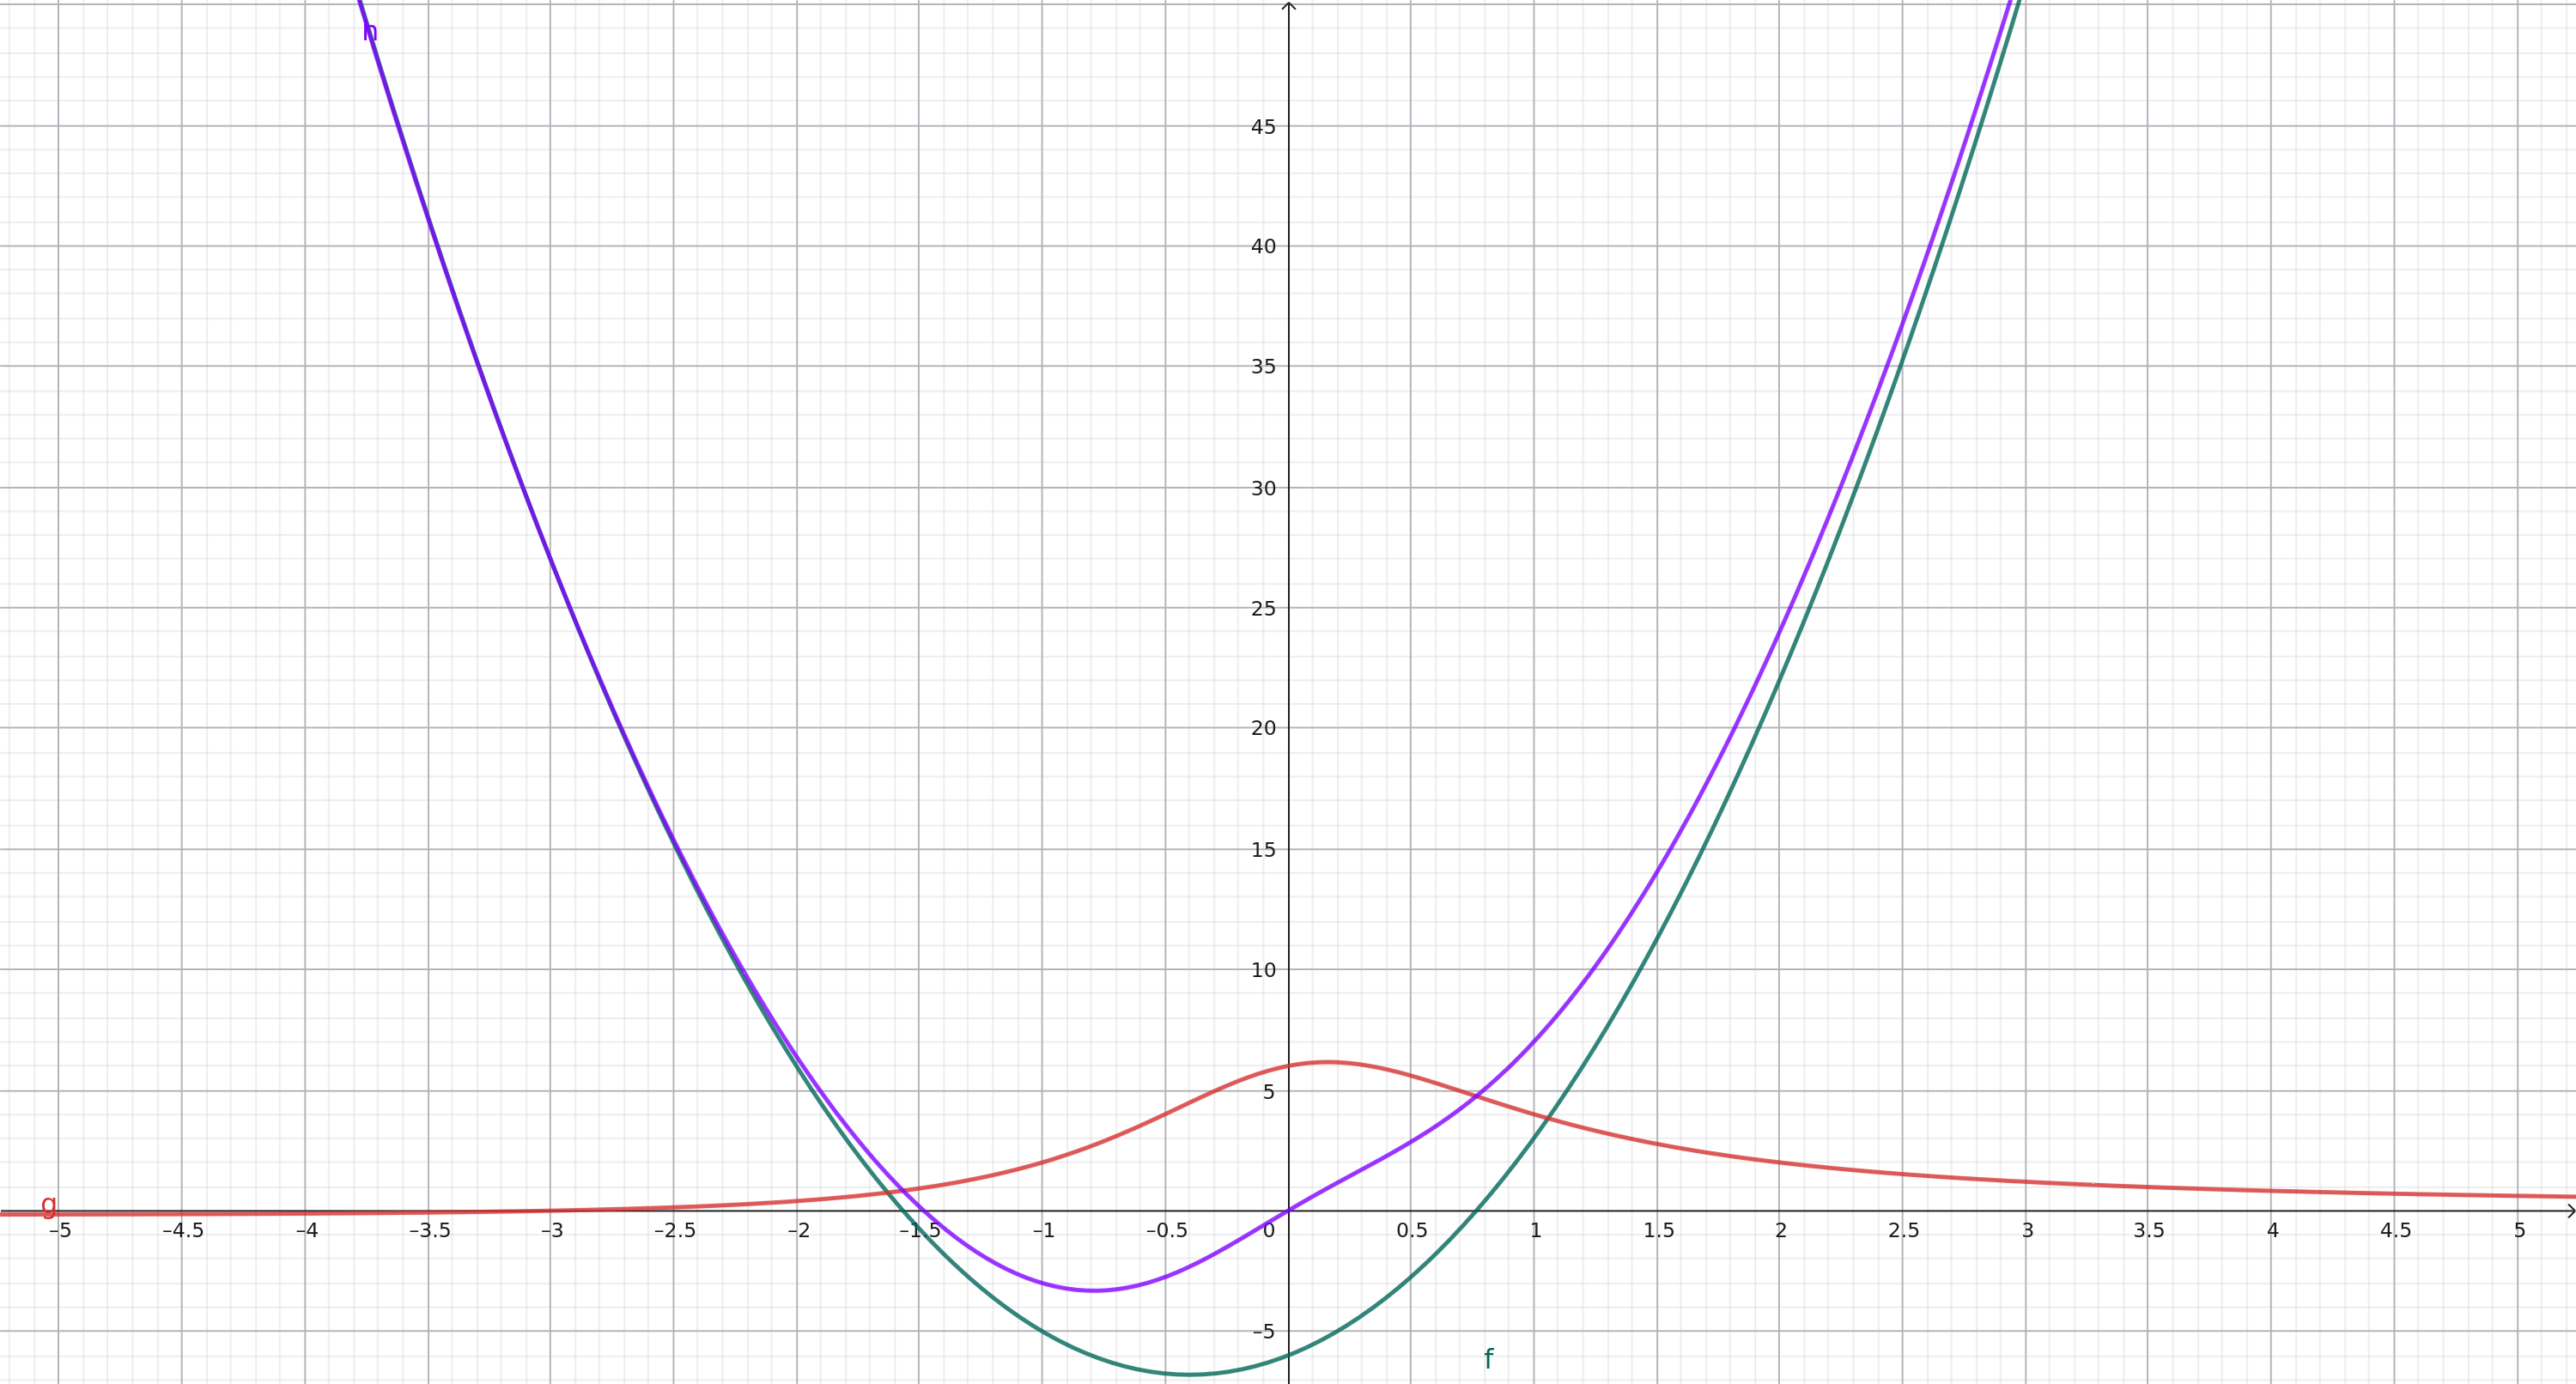
\includegraphics[height=6cm]{racional.png}
\end{center}
\end{ejemplo}

\section{Descomposición en factores irreducibles}

En esta sección desarrollamos más la analogía entre el conjunto de los números enteros y el de los polinomios.

\subsection{Divisibilidad}

\begin{defn}
Si $r=\theta$, entonces decimos que {\bf $q$ divide a $p$} y que {\bf $p$ es divisible por $d$}.
En otras palabras, decimos que $d$ divide a $p$ si existe un polinomio $q$ tal que 
$$p=rd.$$
\end{defn}

Esta noción de divisibilidad es análoga a la divisibilidad de números enteros, y nos conduce a una noción análoga a la de primalidad.

\subsection{Irreducibilidad}

\begin{defn}
Un polinomio $p$ de grado mayor o igual a 1 se dice  {\bf reducible} en $\mathcal{P}(\R)$ si existen dos polinomios $q, s\in \mathcal{P}(\R)$, con $gr(q)\ge 1$ y $ gr(s)\ge 1$, tales  que $p=q s$.

En caso contrario se dice que $p$ es {  {\bf irreducible o primo}} en $\mathcal{P}(\R)$.
\end{defn}


Notamos la importancia de pedir que los grados de $q$ y $s$ sean mayores o iguales a 1, ya que si $q$ o $s$ tuvieran grado 0, serían polinomios constantes, y todos los polinomios se pueden siempre escribir como multiplicación de un polinomio constante por otro polinomio, por ejemplo:

$$ x^2+2=\frac{1}{5}\cdot (5x^2+10),$$

Así, si $p$ es reducible, entonces $gr(p)=gr(q)+gr(s)\ge 2$, todos los polinomios reducibles tienen grado mayor o a igual a 2.

\medskip

\begin{rem}
 Los polinomios de grado 1, $p(x)=a_0+a_1x$,  son todos irreducibles.
\end{rem}

\subsection{Teorema de descomposición prima}

\begin{thm}[{Teorema de descomposición prima.}]
Todo polinomio  $\displaystyle p(x) \in \mathcal{P}(\R)$ admite una única descomposici\'on como producto de polinomios irreducibles mónicos, es decir, existen únicos $p_1, p_2,...,p_m\,\in\R$ mónicos irreducibles y $C\in \R$ tales que:
\[
p(x)=Cp_1(x)p_2(x)\cdots p_m(x);
\]
\end{thm}

Al igual que el teorema análogo que se tiene en los números naturales, este teorema es extremadamente útil, y de él se desprenden varias consecuencias.
Para comenzar, observamos que los divisores de un polinomio, son todos parte de su descomposición única en polinomios irreducibles.

\subsection{Teorema del Factor}

La principal consecuencia de esto tiene relación con las raíces de $p$. Tenemos que $p(x)$ será igual a 0, si y solo sí existe $i\in\{1,\dots,m\}$ tal que $p_i(x)=0$, en otras palabras, $x$ es raíz de $p$ si y solo si $x$ es raíz de alguno de los factores de $p$.
Esto da lugar a los siguientes corolarios.

\medskip

\begin{cor}
Si $p$ es irreducible en $\mathcal{P}(\R)$, entonces  no tiene raíces reales o bien es de grado 1 y tiene una sola.
\end{cor}

De lo anterior deducimos que todas las raíces de un polinomio son raíces de alguno de sus factores irreducibles de grado 1, de donde se obtiene el siguiente teorema.

\medskip

\begin{thm}[Teorema del Factor]
Un polinomio $p$ tiene a $c$ como raíz si y solo si el polinomio $d(x)=x-c$ es factor de $p$.
\end{thm}

En otras palabras:
\begin{eqnarray*}
p(c)=0 &\Longleftrightarrow& \exists\, q\in  \mathcal{P}(\R),\ \forall x\in \R,\  p(x)=q(x)(x-c).\\
&\Longleftrightarrow&d(x)=x-c\textrm{ divide a } p
\end{eqnarray*}

Si analizamos el grado de $p$ y usamos el teorema de descomposición única, obtenemos lo siguiente:

$$ gr(p)=\sum_{i=1}^m gr(p_i).$$

Dado que cada raíz está asociada a al menos un factor de grado 1, obtenemos el siguiente corolario.

\medskip

\begin{cor}
Un polinomio $p$ tiene a lo m\'as $gr(p)$ ra{\'\i}ces distintas.
\end{cor}

El cual, a su vez, nos lleva al siguiente corolario.

\medskip

\begin{cor}
Si dos polinomios $p$ y $q$, de grado $n$, coinciden en $n+1$ puntos distintos, entonces son iguales: $p=q$. 
\end{cor}



\subsection{Multiplicidad de una raíz}

Ahora bien, el factor $d(x)=x-c$ puede figurar en la descomposición única de $p$ con un exponente mayor a 1.
Sea $k\in \N$ el mayor natural tal que $(x-c)^k$ divide a $p$.
Es decir, tomemos $q \in \mathcal{P}(\R)$ no divisible por $(x-c)$ tal que 

\vspace{-.3cm}

$$\forall x\in \R, \quad p(x)=q(x)(x-c)^k.$$

\vspace{-.1cm}

En tal caso decimos que \emph{$c$ es una ra\'iz de multiplicidad $k$.}
Si $k=1$ se dice que $c$ es una {\bf ra\'iz} simple.

\medskip

\begin{rem}
La suma de las multiplicidades de todas las ra\'ices de $p$ es menor o igual que $gr(p)$.
\end{rem}


\section{Teorema del resto}

La división Euclidiana es particularmente interesante cuando dividimos por un polinomio de grado 1, ya que en ese caso, el resto, al tener grado 0 no ser nulo, es una constante. 
El siguiente teorema expresa esto detallando la constante en cuestión.

\medskip

\begin{thm}
El resto de dividir  $p \in \mathcal{P}(\R)$ por  $(x-c)$ es $p(c)$.
\end{thm}

La demostración es interesante, si $q$, $r$ son el cuociente y el resto de dividir $p$ por $x-c$, respectivamente, entonces, por lo dicho antes, $r(x)=a$, con $a$ una constante en $\R$.
Así:
$$ p(x)=q(x)(x-c)+a,$$
y
$$ p(c)=q(c)(c-c)+a=0+a=a.$$
Es decir, la constante $a$ es igual al valor de $p$ en $c$.

Si $c$ es una raíz de $p$, entonces $a=0$, y $(x-c)$ divide a $p$ (como ya habíamos discutido).

Si $c$ no es raíz de $p$, el teorema de todas formas nos sirve para conocer el valor de $p$ en $c$, evaluar el polinomio $p$ en $x=c$, y resulta que hacer la división Euclidiana de $p$ en $(x-c)$ puede ser una forma computacionalmente eficiente de evaluar $p$ en $c$, conocida como Método de Ruffini o división sintética.

\section{Localización de raíces en $\R$}

El siguiente teorema no se puede demostrar con las herramientas que hemos visto en este curso, pero es de gran utilidad, pues nos acota el espacio donde buscar las raíces de $p$.
En general estas raíces las buscaremos mediante métodos computacionales iterativos que solo podrán darnos un valor aproximado de la raíz, y para ello es muy importante saber de antemano en qué intervalo debemos buscar las raíces, este teorema nos da justamente eso.

\begin{thm}
Si $c\in \R$ es ra{\'\i}z de $\displaystyle p(x)=\sum_{i=0}^n a_ix^i$, con $a_0,\dots,a_n\in\R$, entonces:
$$\frac{|a_0|}{\alpha+|a_0|}\le |c|\le \frac{\beta+|a_n|}{|a_n|},$$
donde:
$\alpha=$m\'ax$\{|a_n|,...,|a_1|\}$ y $\beta=$m\'ax$\{|a_{n-1}|,...,|a_0|\}$.
\end{thm}

\medskip

\begin{ejemplo}
Si aplicamos este teorema al polinomio $p(x)=x^3-3x^2-x+3$, vemos que $\alpha=1$, $\beta=3$, $a_0=3$, $n=3$ y $a_n=1$, por lo tanto  $\frac{1}{2} \le |c| \le 4$; todas las raíces de $p$ se encuentran en $[-4,-\frac{1}{2}]\cup[\frac{1}{2},4]$.
\end{ejemplo}



\section{Raíces complejas de un polinomio a coeficientes reales}

Aunque $p$ tenga coeficientes reales, podemos aplicarlo a valores complejos, es decir, verlo como una función $p:\C\rightarrow \C$.
Allí también nos va a interesar qué valores complejos hacen que $p$ se anule, es decir, nos van a interesar sus \emph{raíces complejas.}

\medskip

\begin{thm}
Sea  $p \in \mathcal{P}(\R)$,  y $z=a+bi\in \C$ (con $a,b\in\R$ y $b\not = 0$). Si $p(z)=0$, entonces $p(\overline{z})=0$ y existe $q\in  \mathcal{P}(\R)$  tal que 
$$\forall\,x\in\R,\ p(x)=q(x)[(x-a)^2+b^2].$$
\end{thm}

En efecto, si $p(x)=\sum_{i=0}^n a_ix^i$, con $a_0,\dots,a_n\in\R$, entonces, como $p(z)=0$:

\begin{eqnarray*}
0&=&\overline{0}\\
&=&\overline{p(z)}\\
&=&\overline{\sum_{i=0}^n a_iz^i}\\
&=&\sum_{i=0}^n \overline{a_iz^i}\\
&=&\sum_{i=0}^n a_i\overline{z^i}\\
&=&\sum_{i=0}^n a_i\overline{z}^i\\
&=&p(\overline{z}).
\end{eqnarray*}

Entonces $x-z$ y $x-\overline{z}$ serían factores de $p$, con lo cual $(x-z)(x-\overline{z})$ es factor de $p$, pero
\begin{eqnarray*}
(x-z)(x-\overline{z})&=&(x-a-bi)(x-a+bi)\\
&=&((x-a)-bi)((x-a)+bi)\\
&=&(x-a)^2-(bi)^2\\
&=&(x-a)^2+b^2.
\end{eqnarray*}
De donde se concluye el teorema.

Dado que $(x-a)^2+b^2$ tiene dos raíces en $\C$, no puede tener raíces en $\R$, es un polinomio irreducible en $\R$.
Podemos desarrollarlo un poco más.

$$(x-a)^2+b^2=x^2-2ax+ (a^2+b^2)$$


\begin{rem}
Si $z=a+bi$ es una ra{\'\i}z compleja de $p$ de multiplicidad $k$, entonces $\overline{z}$ tambi\'en lo es, con la misma multiplicidad y el polinomio $[(x-a)^2+b^2]^k$ es un factor de $p$ de grado $2k$.
\end{rem}


\subsection{Teorema fundamental del álgebra}

El siguiente es el teorema más importante del capítulo. Su demostración requiere herramientas de cálculo complejo, y por lo tanto no podemos desarrollarla en este apunte.
Este teorema se refiere a polinomios cuyo coeficientes pueden ser reales o complejos.
Habíamos visto que en $\R$ existen polinomio que no tiene ninguna raíz real, por ejemplo $x^2 +1$.
Esto no ocurren en $\C$, todos los polinomios a coeficientes en $\C$ tienen al menos una raíz en $\C$.
Todas las ecuaciones polinomiales a coeficientes en $\C$ tienen soluciones en $\C$.

\medskip

\begin{thm}
Todo polinomio $p\in\mathcal{P}(\C)$ tiene al menos una raíz en $\C$.
\end{thm}

La principal consecuencia de esto es que en $\C$ los únicos polinomios irreducibles son los polinomios de grado 1.

Como $\R\subseteq \C$, podemos aplicar el teorema también a los polinomios a coeficientes en $\R$.


\medskip

\begin{thm}
Todo polinomio $p\in\mathcal{P}(\R)$ tiene al menos una raíz en $\C$.
\end{thm}

Del análisis anterior, sabemos que cada raíz compleja de $p\in\mathcal{P}(\R)$ arroja un factor de grado par de $p$, con lo cual, si  $p$ tiene grado impar, ha de tener al menos un factor $q$ de grado impar.

El teorema fundamental del álgebra nos dice que $q$ también tiene al menos una raíz, tal raíz es también raíz de $p$, y como ya hemos considerado todas las raíces complejas de $p$, concluimos que las raíces de $q$ han de ser toda reales, y al ser $q$ de grado impar, tiene grado mayor o igual a 1, con lo cual, tiene al menos una raíz.
Que es justo lo que afirma el siguiente corolario.

\medskip

\begin{cor}
 Si $p\in  \mathcal{P}(\R)$ tiene grado impar, entonces $p$ tiene al menos una ra{\'\i}z.
\end{cor}

\medskip

\begin{ejemplo}
Podemos descomponer $p(x)=x^6-1$ en factores irreducibles.
\[
\begin{array}{rl}
p(x)&=x^6-1\\
	&=(x^3-1)(x^3+1)\\
	&=(x-1)(x^2+x+1)(x+1)(x^2-x+1).
\end{array}
\]
Como $x^2+x+1$ y $x^2-x+1$ tienen ra\'ices complejas, concluimos que la descomposición en factores irreducibles de $p$ es:
\[
p(x)=(x-1)(x^2+x+1)(x+1)(x^2-x+1).
\]
De donde sus raíces reales son $1$ y $-1$, mientras que sus raíces complejas son: $\frac{-1+i\sqrt{3}}{2}$ y $\frac{-1-i\sqrt{3}}{2}$.

\end{ejemplo}

\newpage

\section{Descomposici\'on en suma de fracciones parciales}

Muchas veces es más fácil analizar una función racional si se puede escribir como suma de fracciones donde el numerador es constante o de grado 1. 
Es útil ya que facilita el cálculo de su primitiva, y es útil ya que facilita el tratamiento de sus asíntotas y por lo tanto su representación gráfica, dominio y recorrido.
La descomposici\'on en suma de fracciones parciales hace justamente esto, logra escribir cualquier fracción de polinomios $\displaystyle\frac{p}{d}$ como suma de un polinomio más una serie de fracciones donde el numerador es a lo más de grado 1.

El procedimiento es como sigue.

\begin{itemize}
\item Si $p, d \in \mathcal{P}(\R)$,  con $gr(p)<gr(d)$ y $q\ne \theta$.  Entonces la funci\'on racional $\displaystyle\frac{p}{d}$ puede descomponerse en sumas de fracciones cuyos denominadores son polinomios obtenidos de la factorizaci\'on de $d$ en polinomios irreducibles en $ \mathcal{P}(\R)$, de la siguiente forma:

\vspace{.5cm}

\begin{itemize}

\item I)  por cada factor lineal de $d$ con potencia $k$, $(ax+b)^k$,  se obtienen los sumandos:
$$\frac{A_1}{(ax+b)}+ \frac{A_2}{(ax+b)^2}+\cdots +\frac{A_n}{(ax+b)^k}.$$
\end{itemize}


\begin{itemize}

\item II)  por cada factor  irreducible cuadr\'atico de $d$ en  $\mathcal{P}(\R)$, con potencia $m$,  $(ax^2+bx+c)^m$, se obtienen los sumandos:
$$\frac{A_1x+B_1}{(ax^2+bx+c)}+ \frac{A_2x+B_2}{(ax^2+bx+c)^2}+ \cdots +\frac{A_mx+B_m}{(ax^2+bx+c)^m}.$$

\end{itemize}

Luego se calculan todos estos coeficientes $A_i$, $B_i$ de manera tal que $\displaystyle\frac{p(x)}{d(x)}$ coincida con la suma de todos los sumandos antes descritos.

\item Si $p, d \in \mathcal{P}(\R)$,  con $gr(p)\ge gr(d)$ y $q\ne \theta$.
Entonces podemos calcular primero el cuociente $q$ y el resto $r$ de la divisi\'on $\displaystyle\frac{p}{d}$ , tales que:
$$\frac{p}{d}=q+\frac{r}{q}, \quad  gr(r)<gr(d),$$
y luego aplicar el procedimiento anterior a $\displaystyle\frac{r}{d}$, ya que $gr(r)<gr(d)$.
\end{itemize}

\medskip

\begin{ejemplo}
Descomponga la fracci\'on en suma de fracciones
parciales
\[
\frac{3x+6}{(x-2)(x+4)}
\]


Los factores del denominador son lineales diferentes

$$\frac{3x+6}{(x-2)(x+ 4 )}= \frac{A}{x-2} + \frac{B}{x+4}$$
De aqu\'i $A=2$ y $B=1$, es decir,
$$ \frac{3x+6}{(x-2)(x+4)} = \frac{2}{x-2} + \frac{1}{x+4}$$

\end{ejemplo}


%%%%%%%%%%%%%%%%%%%%%%%%%%%%%%%%%%%%%%%%%%%%%%%%%%%%%%%%%%%%%%%%%%%%%%%%%%%
\begin{ejemplo}
Descomponga la fracci\'on en suma de fracciones
parciales
\[
\frac{6x^{2}-14x - 27}{(x+2)(x-3)^{2}}
\]


El denominador tiene el primer factor lineal no repetido y el segundo lineal repetido
\[
\frac{6x^{2}-14x -27}{(x+2)(x-3)^{2}} = \frac{A}{x+2} + \frac{B}{x-3} + \frac{C}{(x-3)^{2}}. 
\]
De aqu\'i $A=1$, $B=5$ y $C=-3$, es decir,
\[
\frac{6x^{2}-14x -27}{(x+2)(x-3)^{2}} = \frac{1}{x+2} + \frac{5}{x-3} - \frac{3}{(x-3) ^{2}}
\]
\end{ejemplo}


%%%%%%%%%%%%%%%%%%%%%%%%%%%%%%%%%%%%%%%%%%%%%%%%%%%%%%%%%%%%%%%%%%%%%%%%%%%
\begin{ejemplo}
Descomponga la fracci\'on en suma de fracciones
parciales
\[
\quad\displaystyle\frac{5x^{2}-8x + 5}{(x-2)(x^{2}-x+1)}
\]


El denominador tiene el primer factor del denominador lineal y el segundo, es
irreducible en los n\'umeros reales
$$\frac{5x^{2}-8x+5}{(x-2)(x^{2}-x+1)} = \frac{A}{x-2} + \frac{Bx+C}{x^{2}-x+1}. $$
De aqu\'i $A=3$, $B=2$ y $C=-1$, es decir,
\[
\frac{5x^{2}-8x+5}{(x-2)(x^{2}-x+1)} = \frac{3}{x-2} + \frac{2x-1}{x^{2}-x+1}
\]
\end{ejemplo}


%%%%%%%%%%%%%%%%%%%%%%%%%%%%%%%%%%%%%%%%%%%%%%%%%%%%%%%%%%%%%%%%%%%%%%%%%%%
\begin{ejemplo}

Descomponga la fracci\'on en suma de fracciones
parciales
\[
\frac{x^{3}-4x^{2}+9x-5}{(x^{2}- 2x + 3)^{2}}
\]

$$\frac{x^{3}-4x^{2}+9x -5}{(x^{2}-2x  +3)^{2}} = \frac{Ax +B}{x^{2}-2x+3} + \frac{Cx +D}{(x^{2}-2x +3)^{2}}$$
De aqu\'i $A=1$, $B=-2$, $C=2$ y  $D = 1$, es decir,
$$\frac{x^{3}- 4x^{2} + 9x - 5}{(x^{2}-2x+3)^{2}} = \frac{x-2}{x^{2}- 2x + 3} + \frac{2x+1}{(x^{2}-2x+3)^{2}}$$

\end{ejemplo}


%%%%%%%%%%%%%%%%%%%%%%%%%%%%%%%%%%%%%%%%%%%%%%%%%%%%%%%%%%%%%%%%%%%%%%%%%%%
\begin{ejemplo}

Descomponga la fracci\'on en suma de fracciones
parciales
\[
\displaystyle\frac{x^{3}- 7x^{2}+ 17x - 17}{x^{2}-5x + 6}
\]

$$\frac{x^{3}- 7x^{2}+17x -17}{x^{2}-5x+6} = x-2 + \frac{x-5}{x^{2}-5x+6}$$
y
$$ \frac{x-5}{x^{2}-5x+6} = \frac{x-5}{(x-2)(x-3)} = \frac{3}{x-2} - \frac{2}{x-3}.$$
Luego
$$\frac{x^{3}-7x^{2}+17x -17} {x^{2}-5x+6} =  (x-2) \,\,+ \,\, \frac{3}{x-2}\,\, - \,\,\frac{2}{x-3}$$
\end{ejemplo}






\end{document}
